\addtocontents{toc}{\protect\setcounter{tocdepth}{1}}
\hypersetup{bookmarksdepth=2}
\chapter{BASIC 65 Command Reference}
\label{cha:basic-reference}


\section{Commands, Functions, and Operators}

This appendix describes each of the commands, functions, and other callable elements of BASIC 65, which is an enhanced version of BASIC 10. Some of these can take one or more arguments, which are pieces of input that you provide as part of the command or function call, to help describe what you want to achieve. Some also require that you use special words.

Below is an example of how commands, functions, and operators (all of which are also known as keywords) will be described in this appendix.

{\bf KEY} number{\bf,} string

Here, {\bf KEY} is a {\em keyword}.\index{Keywords} Keywords are special words that BASIC understands. In this manual, keywords are always written in {\bf BOLD CAPITALS}, so that you can easily recognise them.

The ``number'' and ``string'' (in non-bold text) are examples of {\em arguments}. You replace these with values or algebraic phrases ({\em expressions}) that represent the data that controls the command's behaviour.

Punctuation and other letters in bold text represent other characters that are typed as they appear. In this example, a comma must appear between the number argument and the string argument.

Here is an example of using the {\bf KEY} command based on this pattern:

\begin{screencode}
KEY 6, "LIST" + CHR$(13)
\end{screencode}

When you see square brackets around arguments, this indicates that the arguments are optional. You are not meant to type the square brackets. Consider this description of the {\bf CIRCLE} command, which accepts optional arguments:

{\bf CIRCLE} xc{\bf,} yc{\bf,} radius [{\bf,} flags {\bf,} start{\bf,} stop]

The following examples of the {\bf CIRCLE} command are both valid. They have different behaviour based on their different arguments.

\begin{screencode}
CIRCLE 100, 150, 30

CIRCLE 100, 150, 30, 0, 45, 135
\end{screencode}

This arrangement of keywords, symbols, and arguments is called {\em syntax}. If you leave something out, or put the wrong thing in the wrong place, the computer will fail to understand the command and report a {\em syntax error}.

There is nothing to worry about if you get an error from the MEGA65. It is just the MEGA65's way of telling you that something isn't quite right, so that you can more easily find and fix the problem. For example, if you omit the comma in the {\bf KEY} command, or replace it with a period, the MEGA65 will respond with a Syntax error, as seen here:

\begin{screencode}
READY.
KEY 8"FISH"

?SYNTAX ERROR
READY.
KEY 8."FISH"

?SYNTAX ERROR
READY.
\end{screencode}

Expressions can be a number value such as \screentext{23.7}, a string value such as \screentext{"HELLO"}, or a more complex calculation that combines values, functions, and operators to describe a number or string value: \screentext{"LIST"+CHR\$(13)}

It is important to use the correct type of expression when writing your programs. If you accidentally use the wrong type, the MEGA65 will display a Type Mismatch error, to say that the type of expression you gave doesn't match what it expected. For example, the following command results in a Type Mismatch error, because \screentext{"POTATO"} is a string expression, and a numeric expression is expected:

\begin{screencode}
KEY "POTATO", "SOUP"
\end{screencode}

Commands are statements that you can use directly from the \screentext{READY.} prompt, or from within a program, for example:

\begin{screencode}
READY.
PRINT "HELLO"
HELLO

READY.
10 PRINT "HELLO"
RUN
HELLO
\end{screencode}

You can place a sequence of statements within a single line by separating them with colons, for example:

\begin{screencode}
PRINT "HELLO" : PRINT "HOW ARE YOU?" : PRINT "HOW IS THE WEATHER?"
HELLO
HOW ARE YOU?
HOW IS THE WEATHER?
\end{screencode}

\subsection{Direct Mode Commands}
\index{BASIC 65 Commands!Direct Mode}
Some commands only work in {\bf direct mode} (sometimes called ``immediate mode''). This means that the command can't be part of a BASIC program, but can be entered directly to the screen. For example, the {\bf RENUMBER} command only works in direct mode, because its function is to renumber the lines of a BASIC program.

In the two {\bf PRINT} examples above, the first was entered in direct mode, whereas the second one was part of a program. The {\bf PRINT} command works in both direct mode and in a program.

\subsection{Command Syntax Descriptions}
The following table describes the other symbols found in command syntax descriptions.

\begin{center}
    \setlength{\def\arraystretch{1.5}\tabcolsep}{6pt}
    \begin{longtable}{|c|L{8cm}|}
        \hline
        \textbf{Symbol} & \textbf{Meaning}\\
        \hline
        \endhead
        [ ] &
        Optional \\
        \hline
        \dots &
        The bracketed syntax can be repeated zero or more times \\
        \hline
        < | > &
        Include one of the choices \\
        \hline
        [ | ] &
        Optionally include one of the choices \\
        \hline
        \{ , \} &
        One or more of the arguments is required. The commas to the left of the last
        argument included are required. Trailing commas must be omitted. See
        {\bf CURSOR} for an example.\\
        \hline
        [\{ , \}] &
        Similar to \{ , \} but all arguments can be omitted\\
        \hline

    \end{longtable}
\end{center}

\subsection{Fonts}
Examples of text that appears on the screen, either typed by you or printed by the MEGA65, appear in the screen font: \screentext{"LIST"+CHR\$(13)}


\newpage
\subsection{BASIC 65 Constants}
\index{BASIC 65 Constants}
\setlength{\tabcolsep}{1mm}

Values that are typed directly into an expression or program are called {\em constants}. The values are ``constant'' because they do not change based on other aspects of the program state.

The following are types of constants that can appear in a BASIC 65 expression.

\begin{center}
\begin{tabular}{|l|l|l|}
\hline
{\bf Type}              & {\bf Example} & {\bf Example} \\
\hline
Decimal Integer         &  \screentext{32000} & \screentext{-55}      \\
Decimal Fixed Point     &  \screentext{3.14}  & \screentext{-7654.321}\\
Decimal Floating Point  &  \screentext{1.5E03}& \screentext{7.7E-02}  \\
Hex                     &  \screentext{\$D020}& \screentext{\$FF}     \\
Binary                  &  \screentext{\%11010010}& \screentext{\%101} \\
String                  &  \screentext{"X"}   & \screentext{"TEXT"}   \\
\hline
\end{tabular}
\end{center}

\subsection{BASIC 65 Variables}
\index{BASIC 65 Variables}

A program manipulates data by storing values in the computer's memory, referring to stored values, and updating them based on logic. In BASIC, elements of memory that store values are called {\em variables}. Each variable has a name, there are separate sets of variable names for each type of value.

For example, the variable \screentext{AA} can store a number value. The variable \screentext{AA\$} can store a string value. Commodore BASIC considers these to be separate variables, even though the names both begin with \screentext{AA}.

One way to store a value in a variable is with the assignment operator ({\bf =}). For example:

\begin{screencode}
AA = 1.95

AA$ = "HELLO, "
\end{screencode}

Variable names must start with a letter, and contain only letters and numbers. They can be of any length, but Commodore BASIC only recognizes the first two letters of the name. \screentext{SPEED} and \screentext{SP} would be considered the same variable.

Variable names cannot contain any of the BASIC keywords. This makes using long names difficult: it is easy to use a keyword accidentally. For example, \screentext{ENFORCEMENT} is not a valid variable name, because {\bf FOR} is a keyword. It is common to use short variable names to avoid these hazards.

A variable can be used within an expression with other constants, variables, functions, and operators. It is substituted with the value that it contains at that point in the program's execution.

\begin{screencode}
10 INPUT "WHAT IS YOUR NAME"; NA$
20 MSG$ = "HELLO, " + NA$ + "!"
30 PRINT MSG$
\end{screencode}

Unlike some programming languages, BASIC variables do not need to be declared before use. A variable has a default value of zero for number type variables, or the empty string (\screentext{""}) for string type variables.

A variable that stores a single value is also known as a {\em scalar variable}. The scalar variable types and their value ranges are as follows.

\setlength{\tabcolsep}{1mm}
\begin{center}
\begin{tabular}{|l|l|l|l|}
\hline
{\bf Type} & {\bf Name Symbol} & {\bf Range}       & {\bf Example}  \\
\hline
Byte       & \screentext{\&}          & 0 .. 255          & \screentext{BY\& = 23}    \\
Integer    & \screentext{\%}          & -32768 .. 32767   & \screentext{I\% = 5}      \\
Real       & none                     & -1E37 .. 1E37     & \screentext{XY = 1/3}     \\
String     & \screentext{\$}          & length = 0 .. 255 & \screentext{AB\$ = "TEXT"}\\
\hline
\end{tabular}
\end{center}

A variable whose name is a single letter followed by the type symbol (or no symbol for real number variables) is a {\em fast variable}. BASIC 65 stores the variable in a way that makes it faster to access or update the value than variables with longer names. It otherwise behaves like any other variable. This is also true for functions defined by {\bf DEF FN}.

\subsection{BASIC 65 Arrays}
\index{BASIC 65 Arrays}

In addition to scalar variables, Commodore BASIC also supports a type of variable that can store multiple values, called an {\em array}.

The following example stores three string values in an array, then uses a {\bf FOR} loop to {\bf PRINT} a message for each element:

\begin{screencode}
10 DIM NA$(3)
20 NA$(0) = "DEFT"
30 NA$(1) = "GARDNERS"
40 NA$(2) = "LYDON"
50 FOR I = 0 TO 2
60 PRINT "HELLO, "; NA$(I); "!"
70 NEXT I
\end{screencode}

Each value in an array is referenced by the name of the array variable and an integer index. For example, \screentext{AA(7)} refers to the element of the array named \screentext{AA()} with index 7. Indexes are ``zero-based:'' the first element in the array has an index of 0. The index can be a numeric expression, which can be a powerful way to operate on multiple elements of data.

All values in an array must be of the same type. The type is indicated in the name of the variable, similar to scalar variables. \screentext{AA()} is an array of real numbers, \screentext{AA\$()} is an array of strings.

Array variable names are considered separate from scalar variable names. The scalar variable \screentext{AA} has no relationship to the array variable \screentext{AA()}.

BASIC needs to know the maximum size of the array before its first use, so that it can allocate the memory for the complete array. A program can declare an array's size using the {\bf DIM} keyword, with the ``dimensions'' of the array. If an array variable is used without an explicit declaration, BASIC allocates a one-dimensional array of 10 elements, and the array cannot be re-dimensioned later (unless you {\bf CLR} all variables).

An array can have multiple dimensions, each with its own index separated by a comma. The array must be declared with the maximum value for each dimension. Keep in mind that BASIC 65 allocates memory for the entire array, so large arrays may be constrained by available memory.

\begin{screencode}
DIM BO$(3, 3)
BO$(1, 1) = "X"
BO$(0, 0) = "O"
BO$(0, 2) = "X"
BO$(1, 0) = "O"
\end{screencode}

\subsection{Screen Text and Colour Arrays}
\label{sec:screentextandcolourarrays}
\index{Screen Text and Colour Arrays}

A BASIC 65 program can place text on the screen in several ways. The {\bf PRINT} command displays a string at the current cursor location, which is especially useful for terminal-like output. The {\bf CURSOR} command moves the cursor to a given position. A program can use these commands together to draw pictures or user interfaces.

A program can access individual characters on the screen using the special built-in arrays \textbf{T@\&()} and \textbf{C@\&()}. These arrays are two-dimensional with indexes corresponding to the column and row of each character on the screen, starting from (0,0) at the top left corner.

\textbf{T@\&(}column{\bf ,} row{\bf )} is the screen code of the character. Screen codes are not the same as PETSCII codes. See appendix \vref{appendix:screencodes} for a list of screen codes.

\textbf{C@\&(}column{\bf ,} row{\bf )} is the colour code of the character. This is an entry number of the system palette. See appendix \vref{appendix:colourtable} for the list of colours in the default system palette. Upper bits also set text attributes, such as blinking.

Similar to regular arrays, the screen and colour array entries can be assigned new values, or used in expressions to refer to their current values.

\begin{screencode}
10 FOR X = 10 TO 30
20 T@&(X, 2) = 1
30 C@&(X, 2) = INT(RND(1) * 16)
40 NEXT X
50 PRINT "COLOUR AT POSITION 15: "; C@&(15, 2)
\end{screencode}

The dimensions of these arrays depend on the current text screen mode. In 80 $\times$ 25 text mode, the column is in the range 0 -- 79, and the row is in the range 0 -- 24. The MEGA65 also supports 80 $\times$ 50 and 40 $\times$ 25 text modes.

\subsection{BASIC 65 Operators}
\index{BASIC 65 Operators}

An {\em operator} is a symbol or keyword that performs a function in an expression. It operates on one or two sub-expressions, called {\em operands}. The operator and its operands {\em evaluate to} the result of the operation.

For example, the {\bf *} (asterisk) operator performs a multiplication of two number operands. The operator and its operands evaluate to the result of the multiplication.

\begin{screencode}
A = 6
PRINT A * 7
\end{screencode}

The {\bf +} (plus) operator has a different meaning depending on the type of the operands. If both operands are numbers, then the operator performs an addition of the numbers. If both operands are strings, then the operator evaluates to a new string that is the concatenation of the operands.

\begin{screencode}
A = 64
PRINT A + 1

A$ = "MEGA"
PRINT A$ + "65"
\end{screencode}

The {\bf -} (minus) operator accepts either one operand or two operands. Given one number operand on the right-hand side, it evaluates to the negation of that number. Given two number operands, one on either side, it evaluates to the subtraction of the second operand from the first operand.

\begin{screencode}
A = 64
PRINT -A

PRINT A - 16
\end{screencode}

The equals symbol ({\bf =}) is used both as an assignment statement and as a relational operator. As an assignment, the {\bf =} symbol is a statement that updates the value of a variable. The left-hand side must be a variable or array element reference, and its type must match the type of the expression on the right-hand side. The assignment is not an operator: it is not part of an expression.

\begin{screencode}
AA = 7
NA$ = "DEFT"
\end{screencode}

As a relational operator, the {\bf =} symbol behaves as an expression. It evaluates the expressions on both sides of the operator, then tests whether the values are equal. If they are equal, the equality operator evaluates to $-1$, BASIC's representation of ``true.'' If they are not equal, the operator evaluates to 0, or ``false.'' The equality expression can be used with an {\bf IF} statement to control program flow, or it can be used as part of a numeric expression. Both expressions must be of the same type.

\begin{screencode}
100 IF X = 99 THEN 130
110 X = X + 1
120 GOTO 100
130 PRINT "DONE."
\end{screencode}

BASIC 65 knows the difference between assignment and equality based on context. Consider this line of code:

\begin{screencode}
A = B = 10
\end{screencode}

BASIC 65 expects a statement, and notices a variable name followed by the {\bf =} symbol. It concludes that this is a statement assigning a value to the number variable \screentext{A}. It then expects a number expression on the right-hand side of the assignment, and notices the {\bf =} symbol is an operator in that expression. It concludes that the operation is an equality test, and proceeds to evaluate the expression and assign the result.

The operators {\bf NOT}, {\bf AND}, {\bf OR} and {\bf XOR} can be used either as logical operators or as boolean operators. A logical operator joins two conditional expressions as operands and evaluates to the logical comparison of their truth values.

\begin{screencode}
IF X = 99 OR Y < 5 THEN 130

IF Y > 10 AND Y < 20 THEN 150
\end{screencode}

A boolean operator accepts two number operands and performs a calculation on the bits of the binary values.

\begin{screencode}
A = 17
PRINT A AND 20
\end{screencode}

Unlike other cases where operators have different behaviours based on how they are used, BASIC 65 does not need to determine whether these operators are behaving as logical operators or boolean operators. Because ``true'' and ``false'' are represented by carefully chosen numbers, the logical operators have the same behaviour whether their operands are conditional expressions or numbers. A ``true'' conditional expression is the number $-1$, which internally is a binary number with all bits set. The logical expression ``true and false'' is equivalent to the binary boolean expression {\tt \%....0000 \& \%....1111}. In this case, the {\bf AND} operator evaluates to 0, which is ``false.''

Conditional expressions evaluating to numbers can be used in some clever programming tricks. Consider this example:

\begin{screencode}
A = A - (B > 7)
\end{screencode}

This statement will increment the value in the \screentext{A} by 1 if the value in \screentext{B} is greater than 7. Otherwise it leaves it unchanged. If the sub-expression \screentext{B > 7} is true, then it evaluates to -1. \screentext{A - (-1)} is equivalent to \screentext{A + 1}. If the sub-expression is false, then it evaluates to 0, and \screentext{A - 0} is equivalent to \screentext{A}.

When multiple operators are used in a single expression, the order in which they are evaluated is specified by {\em precedence}. For example, in the statement \screentext{A * A - B * B}, both multiplications will be performed first, then the subtraction. As in algebra, you can use parentheses to change the order of execution. In the expression \screentext{A * (A - B) * B}, the subtraction is performed first.

The complete set of operators and their order of precedence are summarised in the sections that follow.

\subsubsection{Assignment Statement}

\setlength{\tabcolsep}{1mm}
\begin{center}
\begin{tabular}{|l|l|l|l|}
\hline
{\bf Symbol} & {\bf Description} & {\bf Examples}\\
\hline
\screentext{=}           & Assignment        & \screentext{A = 42}, \screentext{A\$ = "HELLO"}, \screentext{A = B < 42}\\
\hline
\end{tabular}
\end{center}

\subsubsection{Unary Mathematical Operators}

\setlength{\tabcolsep}{1mm}
\begin{center}
\begin{tabular}{|l|l|l|l|l|}
\hline
{\bf Name} & {\bf Symbol}   & {\bf Description} & {\bf Example}\\
\hline
Plus       & \screentext{+} & Positive sign     & \screentext{A = +42} \\
Minus      & \screentext{-} & Negative sign     & \screentext{B = -42} \\
\hline
\end{tabular}
\end{center}

\subsubsection{Binary Mathematical Operators}

\setlength{\tabcolsep}{1mm}
\begin{center}
\begin{tabular}{|l|l|l|l|l|}
\hline
{\bf Name}     & {\bf Symbol}     & {\bf Description} & {\bf Example}\\
\hline
Plus           & \screentext{+}   & Addition          & \screentext{A = B + 42}\\
Minus          & \screentext{-}   & Subtraction       & \screentext{B = A - 42}\\
Asterisk       & \screentext{*}   & Multiplication    & \screentext{C = A * B}\\
Slash          & \screentext{/}   & Division          & \screentext{D = B / 13}\\
Up Arrow       & \screentext{$\uparrow$} & Exponentiation    & \screentext{E = 2 $\uparrow$ 10}\\
Left Shift     & \screentext{<<}   & Left Shift        & \screentext{A = B << 2} \\
Right Shift    & \screentext{>>}   & Right Shift       & \screentext{A = B >> 1} \\
\hline
\end{tabular}
\end{center}

\underline{NOTE}: The \screentext{$\uparrow$} character used for exponentiation is entered with \megakeywhite{$\uparrow$}, which is next to \widekey{RESTORE}.

\subsubsection{Relational Operators}

\setlength{\tabcolsep}{1mm}
\begin{center}
\begin{tabular}{|l|l|l|l|}
\hline
{\bf Symbol}    & {\bf Description}        & {\bf Example}\\
\hline
\screentext{>}  & Greater Than             & \screentext{A > 42}  \\
\screentext{>=} & Greater Than or Equal To & \screentext{B >= 42} \\
\screentext{<}  & Less Than                & \screentext{A < 42}  \\
\screentext{<=} & Less Than or Equal To    & \screentext{B <= 42} \\
\screentext{=}  & Equal                    & \screentext{A = 42}  \\
\screentext{<>} & Not Equal                & \screentext{B <> 42} \\
\hline
\end{tabular}
\end{center}

\subsubsection{Logical Operators}

\setlength{\tabcolsep}{1mm}
\begin{center}
\begin{tabular}{|l|l|l|l|}
\hline
{\bf Keyword}     & {\bf Description} & {\bf Example}\\
\hline
\screentext{AND}  & And               & \screentext{A > 42 AND A < 84} \\
\screentext{OR}   & Or                & \screentext{A > 42 OR  A = 0} \\
\screentext{XOR}  & Exclusive Or      & \screentext{A > 42 XOR B > 42} \\
\screentext{NOT}  & Negation          & \screentext{C = NOT A > B} \\
\hline
\end{tabular}
\end{center}

\subsubsection{Boolean Operators}

\setlength{\tabcolsep}{1mm}
\begin{center}
\begin{tabular}{|l|l|l|l|}
\hline
{\bf Keyword}     & {\bf Description} & {\bf Example}\\
\hline
\screentext{AND}  & And               & \screentext{A = B AND \$FF} \\
\screentext{OR}   & Or                & \screentext{A = B OR \$80} \\
\screentext{XOR}  & Exclusive Or      & \screentext{A = B XOR 1} \\
\screentext{NOT}  & Negation          & \screentext{A = NOT 22} \\
\hline
\end{tabular}
\end{center}

\subsubsection{String Operator}

\setlength{\tabcolsep}{1mm}
\begin{center}
\begin{tabular}{|l|l|l|l|l|}
\hline
{\bf Name} & {\bf Symbol}   & {\bf Description}    & {\bf Operand type} & {\bf Example}\\
\hline
Plus       & \screentext{+} & Concatenates Strings & String             & \screentext{A\$ = B\$ + ".PRG"} \\
\hline
\end{tabular}
\end{center}

\subsection{Operator Precedence}

\setlength{\tabcolsep}{1mm}
\begin{center}
\begin{tabular}{|l|l|}
\hline
{\bf Precedence} & {\bf Operators}\\
\hline
High             & \screentext{$\uparrow$} \\
                 & \screentext{+ -} (Unary Mathematical) \\
                 & \screentext{* /} \\
                 & \screentext{+ -} (Binary Mathematical)\\
                 & \screentext{<< >>} (Arithmetic Shifts)\\
                 & \screentext{< <= > >= = <>} \\
                 & \screentext{NOT} \\
                 & \screentext{AND} \\
Low              & \screentext{OR XOR}\\
\hline
\end{tabular}
\end{center}

% Generated by mega65-rom/tools/keywordref.py\newpage
\subsection{Keywords And Tokens Part 1}
{\ttfamily
\setlength{\tabcolsep}{1mm}
\begin{center}
\begin{tabular}{|p{2.2cm}r|p{2.2cm}r|p{2.2cm}r|}
\hline
*          &   AC & COLLISION  & FE17 & EXP        &   BD \\
+          &   AA & COLOR      &   E7 & FAST       & FE25 \\
-          &   AB & CONCAT     & FE13 & FGOSUB     & FE48 \\
/          &   AD & CONT       &   9A & FGOTO      & FE47 \\
<          &   B3 & COPY       &   F4 & FILTER     & FE03 \\
<<         & FE52 & COS        &   BE & FIND       & FE2B \\
=          &   B2 & CURSOR     & FE41 & FN         &   A5 \\
>          &   B1 & CUT        &   E4 & FONT       & FE46 \\
>>         & FE53 & DATA       &   83 & FOR        &   81 \\
ABS        &   B6 & DCLEAR     & FE15 & FOREGROUND & FE39 \\
AND        &   AF & DCLOSE     & FE0F & FORMAT     & FE37 \\
APPEND     & FE0E & DEC        &   D1 & FRE        &   B8 \\
ASC        &   C6 & DECBIN     & CE11 & FREAD\#    & FE1C \\
ATN        &   C1 & DEF        &   96 & FREEZER    & FE4A \\
AUTO       &   DC & DELETE     &   F7 & FWRITE\#   & FE1E \\
BACKGROUND & FE3B & DIM        &   86 & GCOPY      & FE32 \\
BACKUP     &   F6 & DIR        &   EE & GET        &   A1 \\
BANK       & FE02 & DISK       & FE40 & GO         &   CB \\
BEGIN      & FE18 & DLOAD      &   F0 & GOSUB      &   8D \\
BEND       & FE19 & DMA        & FE1F & GOTO       &   89 \\
BLOAD      & FE11 & DMODE      & FE35 & GRAPHIC    &   DE \\
BOOT       & FE1B & DO         &   EB & HEADER     &   F1 \\
BORDER     & FE3C & DOPEN      & FE0D & HELP       &   EA \\
BOX        &   E1 & DOT        & FE4C & HEX\$      &   D2 \\
BSAVE      & FE10 & DPAT       & FE36 & HIGHLIGHT  & FE3D \\
BUMP       & CE03 & DSAVE      &   EF & IF         &   8B \\
BVERIFY    & FE28 & DVERIFY    & FE14 & IMPORT     &   DD \\
CATALOG    & FE0C & ECTORY     & FE29 & INFO       & FE4D \\
CHANGE     & FE2C & EDIT       & FE45 & INPUT      &   85 \\
CHAR       &   E0 & EDMA       & FE21 & INPUT\#    &   84 \\
CHDIR      & FE4B & ELLIPSE    & FE30 & INSTR      &   D4 \\
CHR\$      &   C7 & ELSE       &   D5 & INT        &   B5 \\
CIRCLE     &   E2 & END        &   80 & JOY        &   CF \\
CLOSE      &   A0 & ENVELOPE   & FE0A & KEY        &   F9 \\
CLR        &   9C & ERASE      & FE2A & LEFT\$     &   C8 \\
CMD        &   9D & ERR\$      &   D3 & LEN        &   C3 \\
COLLECT    &   F3 & EXIT       &   ED & LET        &   88 \\
\hline
\end{tabular}
\end{center}
}
\newpage
\subsection{Keywords And Tokens Part 2}
{\ttfamily
\setlength{\tabcolsep}{1mm}
\begin{center}
\begin{tabular}{|p{2.2cm}r|p{2.2cm}r|p{2.2cm}r|}
\hline
LINE       &   E5 & PRINT      &   99 & SPEED      & FE26 \\
LIST       &   9B & PRINT\#    &   98 & SPRCOLOR   & FE08 \\
LOAD       &   93 & RCOLOR     &   CD & SPRITE     & FE07 \\
LOADIFF    & FE43 & RCURSOR    & FE42 & SPRSAV     & FE16 \\
LOCK       & FE50 & READ       &   87 & SQR        &   BA \\
LOG        &   BC & RECORD     & FE12 & STEP       &   A9 \\
LOG10      & CE08 & REM        &   8F & STOP       &   90 \\
LOOP       &   EC & RENAME     &   F5 & STRBIN\$   & CE12 \\
LPEN       & CE04 & RENUMBER   &   F8 & STR\$      &   C4 \\
MEM        & FE23 & RESTORE    &   8C & SYS        &   9E \\
MERGE      &   E6 & RESUME     &   D6 & TAB(       &   A3 \\
MID\$      &   CA & RETURN     &   8E & TAN        &   C0 \\
MKDIR      & FE51 & RGRAPHIC   &   CC & TEMPO      & FE05 \\
MOD        & CE0B & RIGHT\$    &   C9 & THEN       &   A7 \\
MONITOR    &   FA & RMOUSE     & FE3F & TO         &   A4 \\
MOUNT      & FE49 & RND        &   BB & TRAP       &   D7 \\
MOUSE      & FE3E & RPALETTE   & CE0D & TROFF      &   D9 \\
MOVSPR     & FE06 & RPEN       &   D0 & TRON       &   D8 \\
NEW        &   A2 & RPLAY      & CE0F & TYPE       & FE27 \\
NEXT       &   82 & RREG       & FE09 & UNLOCK     & FE4F \\
NOT        &   A8 & RSPCOLOR   & CE07 & UNTIL      &   FC \\
OFF        & FE24 & RSPEED     & CE0E & USING      &   FB \\
ON         &   91 & RSPPOS     & CE05 & USR        &   B7 \\
OPEN       &   9F & RSPRITE    & CE06 & VAL        &   C5 \\
OR         &   B0 & RUN        &   8A & VERIFY     &   95 \\
PAINT      &   DF & RWINDOW    & CE09 & VIEWPORT   & FE31 \\
PALETTE    & FE34 & SAVE       &   94 & VOL        &   DB \\
PASTE      &   E3 & SAVEIFF    & FE44 & VSYNC      & FE54 \\
PEEK       &   C2 & SCNCLR     &   E8 & WAIT       &   92 \\
PEN        & FE33 & SCRATCH    &   F2 & WHILE      &   FD \\
PIXEL      & CE0C & SCREEN     & FE2E & WINDOW     & FE1A \\
PLAY       & FE04 & SET        & FE2D & WPEEK      & CE10 \\
POINTER    & CE0A & SGN        &   B4 & WPOKE      & FE1D \\
POKE       &   97 & SIN        &   BF & XOR        &   E9 \\
POLYGON    & FE2F & SLEEP      & FE0B & \string^   &   AE \\
POS        &   B9 & SOUND      &   DA &            &      \\
POT        & CE02 & SPC(       &   A6 &            &      \\
\hline
\end{tabular}
\end{center}
}
\newpage
\subsection{Tokens And Keywords Part 1}
{\ttfamily
\setlength{\tabcolsep}{1mm}
\begin{center}
\begin{tabular}{|rp{2.2cm}|rp{2.2cm}|rp{2.2cm}|}
\hline
  80 & END        &   A5 & FN         &   CA & MID\$      \\
  81 & FOR        &   A6 & SPC(       &   CB & GO         \\
  82 & NEXT       &   A7 & THEN       &   CC & RGRAPHIC   \\
  83 & DATA       &   A8 & NOT        &   CD & RCOLOR     \\
  84 & INPUT\#    &   A9 & STEP       & CE02 & POT        \\
  85 & INPUT      &   AA & +          & CE03 & BUMP       \\
  86 & DIM        &   AB & -          & CE04 & LPEN       \\
  87 & READ       &   AC & *          & CE05 & RSPPOS     \\
  88 & LET        &   AD & /          & CE06 & RSPRITE    \\
  89 & GOTO       &   AE & \string^   & CE07 & RSPCOLOR   \\
  8A & RUN        &   AF & AND        & CE08 & LOG10      \\
  8B & IF         &   B0 & OR         & CE09 & RWINDOW    \\
  8C & RESTORE    &   B1 & >          & CE0A & POINTER    \\
  8D & GOSUB      &   B2 & =          & CE0B & MOD        \\
  8E & RETURN     &   B3 & <          & CE0C & PIXEL      \\
  8F & REM        &   B4 & SGN        & CE0D & RPALETTE   \\
  90 & STOP       &   B5 & INT        & CE0E & RSPEED     \\
  91 & ON         &   B6 & ABS        & CE0F & RPLAY      \\
  92 & WAIT       &   B7 & USR        & CE10 & WPEEK      \\
  93 & LOAD       &   B8 & FRE        & CE11 & DECBIN     \\
  94 & SAVE       &   B9 & POS        & CE12 & STRBIN\$   \\
  95 & VERIFY     &   BA & SQR        &   CF & JOY        \\
  96 & DEF        &   BB & RND        &   D0 & RPEN       \\
  97 & POKE       &   BC & LOG        &   D1 & DEC        \\
  98 & PRINT\#    &   BD & EXP        &   D2 & HEX\$      \\
  99 & PRINT      &   BE & COS        &   D3 & ERR\$      \\
  9A & CONT       &   BF & SIN        &   D4 & INSTR      \\
  9B & LIST       &   C0 & TAN        &   D5 & ELSE       \\
  9C & CLR        &   C1 & ATN        &   D6 & RESUME     \\
  9D & CMD        &   C2 & PEEK       &   D7 & TRAP       \\
  9E & SYS        &   C3 & LEN        &   D8 & TRON       \\
  9F & OPEN       &   C4 & STR\$      &   D9 & TROFF      \\
  A0 & CLOSE      &   C5 & VAL        &   DA & SOUND      \\
  A1 & GET        &   C6 & ASC        &   DB & VOL        \\
  A2 & NEW        &   C7 & CHR\$      &   DC & AUTO       \\
  A3 & TAB(       &   C8 & LEFT\$     &   DD & IMPORT     \\
  A4 & TO         &   C9 & RIGHT\$    &   DE & GRAPHIC    \\
\hline
\end{tabular}
\end{center}
}
\newpage
\subsection{Tokens And Keywords Part 2}
{\ttfamily
\setlength{\tabcolsep}{1mm}
\begin{center}
\begin{tabular}{|rp{2.2cm}|rp{2.2cm}|rp{2.2cm}|}
\hline
  DF & PAINT      & FE08 & SPRCOLOR   & FE2F & POLYGON    \\
  E0 & CHAR       & FE09 & RREG       & FE30 & ELLIPSE    \\
  E1 & BOX        & FE0A & ENVELOPE   & FE31 & VIEWPORT   \\
  E2 & CIRCLE     & FE0B & SLEEP      & FE32 & GCOPY      \\
  E3 & PASTE      & FE0C & CATALOG    & FE33 & PEN        \\
  E4 & CUT        & FE0D & DOPEN      & FE34 & PALETTE    \\
  E5 & LINE       & FE0E & APPEND     & FE35 & DMODE      \\
  E6 & MERGE      & FE0F & DCLOSE     & FE36 & DPAT       \\
  E7 & COLOR      & FE10 & BSAVE      & FE37 & FORMAT     \\
  E8 & SCNCLR     & FE11 & BLOAD      & FE39 & FOREGROUND \\
  E9 & XOR        & FE12 & RECORD     & FE3B & BACKGROUND \\
  EA & HELP       & FE13 & CONCAT     & FE3C & BORDER     \\
  EB & DO         & FE14 & DVERIFY    & FE3D & HIGHLIGHT  \\
  EC & LOOP       & FE15 & DCLEAR     & FE3E & MOUSE      \\
  ED & EXIT       & FE16 & SPRSAV     & FE3F & RMOUSE     \\
  EE & DIR        & FE17 & COLLISION  & FE40 & DISK       \\
  EF & DSAVE      & FE18 & BEGIN      & FE41 & CURSOR     \\
  F0 & DLOAD      & FE19 & BEND       & FE42 & RCURSOR    \\
  F1 & HEADER     & FE1A & WINDOW     & FE43 & LOADIFF    \\
  F2 & SCRATCH    & FE1B & BOOT       & FE44 & SAVEIFF    \\
  F3 & COLLECT    & FE1C & FREAD\#    & FE45 & EDIT       \\
  F4 & COPY       & FE1D & WPOKE      & FE46 & FONT       \\
  F5 & RENAME     & FE1E & FWRITE\#   & FE47 & FGOTO      \\
  F6 & BACKUP     & FE1F & DMA        & FE48 & FGOSUB     \\
  F7 & DELETE     & FE21 & EDMA       & FE49 & MOUNT      \\
  F8 & RENUMBER   & FE23 & MEM        & FE4A & FREEZER    \\
  F9 & KEY        & FE24 & OFF        & FE4B & CHDIR      \\
  FA & MONITOR    & FE25 & FAST       & FE4C & DOT        \\
  FB & USING      & FE26 & SPEED      & FE4D & INFO       \\
  FC & UNTIL      & FE27 & TYPE       & FE4F & UNLOCK     \\
  FD & WHILE      & FE28 & BVERIFY    & FE50 & LOCK       \\
FE02 & BANK       & FE29 & ECTORY     & FE51 & MKDIR      \\
FE03 & FILTER     & FE2A & ERASE      & FE52 & <<         \\
FE04 & PLAY       & FE2B & FIND       & FE53 & >>         \\
FE05 & TEMPO      & FE2C & CHANGE     & FE54 & VSYNC      \\
FE06 & MOVSPR     & FE2D & SET        &      &            \\
FE07 & SPRITE     & FE2E & SCREEN     &      &            \\
\hline
\end{tabular}
\end{center}
}



\newpage
\section{BASIC Command Reference}


% =======================================
% Start of the BASIC 65 command reference
% =======================================

\titleformat*{\subsection}{\normalfont\huge\bfseries\color{blue}}

% ***
% ABS
% ***

\newpage
\subsection{ABS}
\index{BASIC 65 Functions!ABS}
\begin{description}[leftmargin=2cm,style=nextline]
\item [Token:]    \$B6

\item [Format:]   {\bf ABS(}x{\bf)}

\item [Returns:]  The absolute value of the numeric argument {\bf x}.

                  {\bf x} numeric integer or real expression argument.

\item [Remarks:]  The result is of type real.

\item [Examples:] Using {\bf ABS}

\begin{tcolorbox}[colback=black,coltext=white]
\verbatimfont{\codefont}
\begin{verbatim}
PRINT ABS(-123)
 123

PRINT ABS(4.5)
 4.5

PRINT ABS(-4.5)
 4.5
\end{verbatim}
\end{tcolorbox}
\end{description}

% ***
% AND
% ***

\newpage
\subsection{AND}
\index{BASIC 65 Operators!AND}
\begin{description}[leftmargin=2cm,style=nextline]
\item [Token:]    \$AF

\item [Format:]   operand {\bf AND} operand

\item [Usage:]    Performs a bit-wise logical AND operation on two 16-bit values.

                  Integer operands are used as they are. Real operands are converted to a signed 16-bit integer (losing precision) in ``two's complement'' format. Logical operands are converted to 16-bit integer using \$FFFF (-1) for TRUE, and \$0000 (0) for FALSE.

                  \begin{center}
                  \setlength{\tabcolsep}{1mm}
                  \begin{tabular}{|c|c|}
                     \hline
                        {\bf Expression} & {\bf Result}  \\
                     \hline
                        \texttt{0 AND 0} & \texttt{0} \\
                        \texttt{0 AND 1} & \texttt{0} \\
                        \texttt{1 AND 0} & \texttt{0} \\
                        \texttt{1 AND 1} & \texttt{1} \\
                     \hline
                  \end{tabular}
                  \end{center}

\item [Remarks:]  The result is of type integer. If the result is used in a logical context, the value of 0 is regarded as FALSE, and all other non-zero values are regarded as TRUE.

\item [Examples:] Using {\bf AND}

\begin{tcolorbox}[colback=black,coltext=white]
\verbatimfont{\codefont}
\begin{verbatim}
PRINT 1 AND 3
 1

PRINT 128 AND 64
 0
\end{verbatim}
\end{tcolorbox}

                  Using {\bf AND} in a logical context ({\bf IF})

\begin{tcolorbox}[colback=black,coltext=white]
\verbatimfont{\codefont}
\begin{verbatim}
IF (C >= 0 AND C < 256) THEN PRINT "BYTE VALUE"
\end{verbatim}
\end{tcolorbox}
\end{description}

% ******
% APPEND
% ******

\newpage
\subsection{APPEND}
\index{BASIC 65 Commands!APPEND}
\begin{description}[leftmargin=2cm,style=nextline]
\item [Token:]    \$FE \$0E

\item [Format:]   {\bf APPEND\#} channel{\bf,} filename [{\bf,D} drive] [{\bf,U} unit]

\item [Usage:]    Opens an existing file of type {\bf SEQ} or {\bf USR} for writing, and positions the write pointer at the end of the file.

                  {\bf channel} number where:
                  \begin{itemize}
                     \item 1 <= channel <= 127: Line terminator is CR.
                     \item 128 <= channel <= 255: Line terminator is CR LF.
                  \end{itemize}

                  \filenamedefinition

                  \drivedefinition

                  \unitdefinition

\item [Remarks:]  {\bf APPEND\#} works similarly to {\bf DOPEN\#... ,W}, except that the file must already exist.

                  The content of the file is retained, and all printed text is appended to the end.
      
                  Trying to {\bf APPEND\#} to a non-existing file reports a DOS error.

\item [Examples:] Using {\bf APPEND\#} (opening existing files)

\begin{tcolorbox}[colback=black,coltext=white]
\verbatimfont{\codefont}
\begin{verbatim}
APPEND#5, "DATA", U9

APPEND#130, (DD$), U(UN%)

APPEND#3, "USER FILE,U"

APPEND#2, "DATA BASE"
\end{verbatim}
\end{tcolorbox}
\end{description}

% ***
% ASC
% ***

\newpage
\subsection{ASC}
\index{BASIC 65 Functions!ASC}
\begin{description}[leftmargin=2cm,style=nextline]
\item [Token:]    \$C6

\item [Format:]   {\bf ASC(}string{\bf)}

\item [Returns:]  The PETSCII code of the first character of the string argument, as a number.

\item [Remarks:]  {\bf ASC} returns zero for empty strings. This is different to BASIC 2, which raised an Illegal Quantity error for empty strings.

                  The inverse function to {\bf ASC} is {\bf CHR\$}. Refer to the {\bf CHR\$} function on page \pageref{BASIC 65 Functions!CHR} for more information.

                  The name was apparently chosen to be a mnemonic to ``ASCII,'' but the returned value is a PETSCII code.

\item [Examples:] Using {\bf ASC}

\begin{tcolorbox}[colback=black,coltext=white]
\verbatimfont{\codefont}
\begin{verbatim}
PRINT ASC("MEGA")
 77

PRINT ASC("")
 0
\end{verbatim}
\end{tcolorbox}
\end{description}

% ***
% ATN
% ***

\newpage
\subsection{ATN}
\index{BASIC 65 Functions!ATN}
\begin{description}[leftmargin=2cm,style=nextline]
\item [Token:]    \$C1

\item [Format:]   {\bf ATN(}numeric expression{\bf)}

\item [Returns:]  The arc tangent of the argument.

                  The result is in the range ($-\pi/2$ to $\pi/2$).

\item [Remarks:]  A multiplication of the result with $180/\pi$ converts the value to the unit "degrees". {\bf ATN} is the inverse function to {\bf TAN}.

\item [Examples:] Using {\bf ATN}

\begin{tcolorbox}[colback=black,coltext=white]
\verbatimfont{\codefont}
\begin{verbatim}
PRINT ATN(0.5)
 0.46364761

PRINT ATN(0.5) * 180 / ~
 26.565051
\end{verbatim}
\end{tcolorbox}
\end{description}

% ****
% AUTO
% ****

\newpage
\subsection{AUTO}
\index{BASIC 65 Commands!AUTO}
\begin{description}[leftmargin=2cm,style=nextline]
\item [Token:]    \$DC

\item [Format:]   {\bf AUTO} [step]

\item [Usage:]    Enables or disables automatic line numbering during BASIC program entry. After submitting a new program line to the BASIC editor with \specialkey{RETURN}, the {\bf AUTO} function generates a new BASIC line number for the entry of the next line. The new number is computed by adding {\bf step} to the current line number.

                  {\bf step} line number increment.

                  Typing {\bf AUTO} with no argument disables it.

\item [Examples:] Using {\bf AUTO}

\begin{tcolorbox}[colback=black,coltext=white]
\verbatimfont{\codefont}
\begin{verbatim}
AUTO 10 : REM USE AUTO WITH INCREMENT 10

AUTO    : REM SWITCH AUTO OFF
\end{verbatim}
\end{tcolorbox}
\end{description}

% **********
% BACKGROUND
% **********

\newpage
\subsection{BACKGROUND}
\index{BASIC 65 Commands!BACKGROUND}
\begin{description}[leftmargin=2cm,style=nextline]
\item [Token:]   \$FE \$3B

\item [Format:]  {\bf BACKGROUND} colour

\item [Usage:]   Sets the background colour of the screen.

                 {\bf colour} palette entry number, in the range 0 -- 255

                 All colours within this range are customisable via the {\bf PALETTE} command.
                 
                 On startup, the MEGA65 only has the first 32 colours configured. See appendix \vref{appendix:colourtable} for the list of colours in the default system palette.

\item [Example:] Using {\bf BACKGROUND}

\begin{tcolorbox}[colback=black,coltext=white]
\verbatimfont{\codefont}
\begin{verbatim}
BACKGROUND 3 : REM SELECT BACKGROUND COLOUR CYAN
\end{verbatim}
\end{tcolorbox}
\end{description}

% ******
% BACKUP
% ******

\newpage
\subsection{BACKUP}
\index{BASIC 65 Commands!BACKUP}
\begin{description}[leftmargin=2cm,style=nextline]
\item [Token:]    \$F6

\item [Format:]   {\bf BACKUP U} source {\bf TO U} target \\
                  {\bf BACKUP D} source {\bf TO D} target [{\bf,U} unit]

\item [Usage:]    Copies one disk to another.

                  The first form of {\bf BACKUP}, specifying units for source and target, can only be used for the drives connected to the internal FDC (Floppy Disk Controller). Units 8 and 9 are reserved for this controller. These can be either the internal floppy drive (unit 8) and another floppy drive (unit 9) attached to the same ribbon cable, or mounted D81 disk images. {\bf BACKUP} can be used to copy from floppy to floppy, floppy to image, image to floppy and image to image, depending on image mounts and the existence of a second physical floppy drive.

                  The second form of {\bf BACKUP}, specifying drives for source and target, is meant to be used for dual drive units connected to the IEC bus. For example: CBM 4040, 8050, 8250 via an IEEE-488 to IEC adapter. In this case, the backup is then done by the disk unit internally.

                  {\bf source} unit or drive \# of source disk.

                  {\bf target} unit or drive \# of target disk.

\item [Remarks:]  The target disk will be formatted and an identical copy of the source disk will be written. 

                  {\bf BACKUP} cannot be used to backup from internal devices to IEC devices or vice versa.

\item [Examples:] Using {\bf BACKUP}

\begin{tcolorbox}[colback=black,coltext=white]
\verbatimfont{\codefont}
\begin{verbatim}
BACKUP U8 TO U9      : REM BACKUP FDC UNIT 8 TO FDC UNIT 9

BACKUP U9 TO U8      : REM BACKUP FDC UNIT 9 TO FDC UNIT 8

BACKUP D0 TO D1, U10 : REM BACKUP ON DUAL DRIVE CONNECTED VIA IEC
\end{verbatim}
\end{tcolorbox}
\end{description}

% ****
% BANK
% ****

\newpage
\subsection{BANK}
\index{BASIC 65 Commands!BANK}
\label{BASIC 65 Commands!BANK}
\begin{description}[leftmargin=2cm,style=nextline]
\item [Token:]    \$FE \$02

\item [Format:]   {\bf BANK} bank number

\item [Usage:]    Selects the memory configuration for BASIC commands that use 16-bit addresses. These are {\bf LOAD}, {\bf LOADIFF}, {\bf PEEK}, {\bf POKE}, {\bf SAVE}, {\bf SYS}, and {\bf WAIT}. Refer to the system memory map in \ifdefined\printmanual
   the {\bf MEGA65 Book}
\else
   \bookvref{cha:memory-map}
\fi for more information.

\item [Remarks:]  A value > 127 selects memory mapped I/O.

                  The default value at system startup for the bank number is 128.

                  This configuration has RAM from \$0000 to \$1FFF, the BASIC and KERNAL ROM, and I/O from \$2000 to \$FFFF.

\item [Example:]  Using {\bf BANK}

\begin{tcolorbox}[colback=black,coltext=white]
\verbatimfont{\codefont}
\begin{verbatim}
BANK 1 : REM SELECT MEMORY CONFIGURATION 1
\end{verbatim}
\end{tcolorbox}
\end{description}

% *****
% BEGIN
% *****

\newpage
\subsection{BEGIN}
\index{BASIC 65 Commands!BEGIN}
\begin{description}[leftmargin=2cm,style=nextline]
\item [Token:]   \$FE \$18

\item [Format:]  {\bf BEGIN} ... {\bf BEND}

\item [Usage:]   The beginning of a compound statement to be executed after {\bf THEN} or {\bf ELSE}. This overcomes the single line limitation of the standard {\bf IF} ... {\bf THEN} ... {\bf ELSE} clause.

\item [Remarks:] Do not jump with {\bf GOTO} or {\bf GOSUB} into a compound statement, as it may lead to unexpected results.

\item [Example:] Using {\bf BEGIN} ... {\bf BEND}

\begin{tcolorbox}[colback=black,coltext=white]
\verbatimfont{\codefont}
\begin{verbatim}
10 GET A$
20 IF A$ >= "A" AND A$ <= "Z" THEN BEGIN : REM IGNORE ALL EXCEPT (A-Z)
30 PW$ = PW$ + A$
40 IF LEN(PW$) > 7 THEN 90
50 BEND
60 IF A$ <> CHR$(13) GOTO 10
90 PRINT "PW="; PW$
\end{verbatim}
\end{tcolorbox}
\end{description}

% ****
% BEND
% ****

\newpage
\subsection{BEND}
\index{BASIC 65 Commands!BEND}
\begin{description}[leftmargin=2cm,style=nextline]
\item [Token:]   \$FE \$19

\item [Format:]  {\bf BEGIN} ... {\bf BEND}

\item [Usage:]   The end of a compound statement to be executed after {\bf THEN} or {\bf ELSE}. This overcomes the single line limitation of the standard {\bf IF} ... {\bf THEN} ... {\bf ELSE} clause.

\item [Remarks:] The example below shows a quirk in the implementation of the compound statement. If the condition evaluates to {\bf FALSE}, execution does not resume right after {\bf BEND} as it should, but at the beginning of the next line.

\item [Example:] Using {\bf BEGIN} ... {\bf BEND}

\begin{tcolorbox}[colback=black,coltext=white]
\verbatimfont{\codefont}
\begin{verbatim}
5 REM DEMOS THE "QUIRK" DESCRIBED
10 IF Z > 1 THEN BEGIN : A$ = "ONE"
20 B$ = "TWO"
30 PRINT A$; " "; B$; : BEND : PRINT " QUIRK"
40 REM EXECUTION RESUMES HERE FOR Z <= 1
\end{verbatim}
\end{tcolorbox}
\end{description}

% *****
% BLOAD
% *****

\newpage
\subsection{BLOAD}
\index{BASIC 65 Commands!BLOAD}
\begin{description}[leftmargin=2cm,style=nextline]
\item [Token:]    \$FE \$11

\item [Format:]   {\bf BLOAD} filename [{\bf,B} bank] [{\bf,P} address] [{\bf,R}] [{\bf,D} drive] [{\bf,U} unit]

\item [Usage:]    Loads a file of type {\bf PRG} into RAM at address {\bf,P}. (``Binary load.'')

                  {\bf BLOAD} has two modes: The flat memory address mode can be used to load a program to any address in the 28-bit (256MB) address range where RAM is installed. This includes the standard RAM banks 0 to 5, as well as the 8MB of "attic RAM" at address \$8000000 (800.0000).

                  This mode is triggered by specifying an address at parameter {\bf P} that is larger than \$FFFF. The bank parameter is ignored in this mode.

                  For compatibility reasons with older BASIC versions, {\bf BLOAD} accepts the syntax with a 16-bit address at P and a bank number at B as well. The attic RAM is out of range for this compatibility mode.

                  The optional parameter {\bf R} (``raw mode'') does not interpret or use the first two bytes of the program file as the load address, which is otherwise the default behaviour. In raw mode, every byte is read as data.

                  \filenamedefinition

                  {\bf bank} specifies the RAM bank to be used. If not specified, the current bank, as set with the last {\bf BANK} statement will be used.

                  {\bf address} overrides the load address that is stored in the first two bytes of the {\bf PRG} file.

                  \drivedefinition

                  \unitdefinition

\item [Remarks:]  {\bf BLOAD} cannot cross bank boundaries.

                  {\bf BLOAD} uses the load address from the file if no {\bf P} parameter is given.

                  It is possible to coerce {\bf BLOAD} to load a file of type {\bf SEQ} by using a filename suffix of: \screentext{",S"}. Be sure to also enable raw mode to avoid treating the first two bytes as a {\bf PRG} load address: \screentext{BLOAD "DATA,S",R,P(\$C000)}

\item [Examples:] Using {\bf BLOAD}

\begin{tcolorbox}[colback=black,coltext=white]
\verbatimfont{\codefont}
\begin{verbatim}
BLOAD "ML DATA", B0, U9

BLOAD "SPRITES"

BLOAD "ML ROUTINES", B1, P32768

BLOAD (FI$), B(BA%), P(PA), U(UN%)

BLOAD "CHUNK", P($8000000)
\end{verbatim}
\end{tcolorbox}
\end{description}

% ****
% BOOT
% ****

\newpage
\subsection{BOOT}
\index{BASIC 65 Commands!BOOT}
\begin{description}[leftmargin=2cm,style=nextline]
\item [Token:]    \$FE \$1B

\item [Format:]   {\bf BOOT} filename [{\bf,B} bank][{\bf,P} address] [{\bf,D} drive] [{\bf,U} unit] \\
                  {\bf BOOT SYS} \\
                  {\bf BOOT}

\item [Usage:]    Loads and runs a program or boot sector from a disk.

                  {\bf BOOT filename} loads a file of type {\bf PRG} into RAM at address {\bf P} and bank {\bf B}, and starts executing the code at the load address.

                  {\bf BOOT SYS} loads the boot sector (512 bytes in total) from sector 0, track 1 and unit 8 to address \$0400 in bank 0, and performs a \texttt{JSR \$0400} afterwards (Jump To Subroutine).

                  {\bf BOOT} with no parameters attempts to load and execute a file named \screentext{AUTOBOOT.C65} from the default unit. It's short for: \screentext{RUN "AUTOBOOT.C65"}

                  \filenamedefinition

                  {\bf bank} specifies the RAM bank to be used. If not specified, the current bank, as set with the last {\bf BANK} statement, will be used.

                  {\bf address} overrides the load address, that is stored in the first two bytes of the {\bf PRG} file.

                  \drivedefinition

                  \unitdefinition

\begin{comment}
\item [Remarks:]  {\bf BOOT SYS} copies the contents of one physical sector (two logical sectors) = 512 bytes from disk to RAM, filling RAM from \$0400 to \$05FF.
\end{comment}

\item [Examples:] Using {\bf BOOT}

\begin{tcolorbox}[colback=black,coltext=white]
\verbatimfont{\codefont}
\begin{verbatim}
BOOT SYS

BOOT (FI$), B(BA%), P(PA), U(UN%)

BOOT
\end{verbatim}
\end{tcolorbox}
\end{description}

% ******
% BORDER
% ******

\newpage
\subsection{BORDER}
\index{BASIC 65 Commands!BORDER}
\begin{description}[leftmargin=2cm,style=nextline]
\item [Token:]   \$FE \$3C

\item [Format:]  {\bf BORDER} colour

\item [Usage:]   Sets the border colour of the screen.

                 {\bf colour} palette entry number, in the range 0 -- 255.

                 All colours within this range are customisable via the {\bf PALETTE} command. See appendix \vref{appendix:colourtable} for the list of colours in the default system palette.

\item [Example:] Using {\bf BORDER}

\begin{tcolorbox}[colback=black,coltext=white]
\verbatimfont{\codefont}
\begin{verbatim}
BORDER 4 : REM SELECT BORDER COLOUR PURPLE
\end{verbatim}
\end{tcolorbox}
\end{description}

% ***
% BOX
% ***

\newpage
\subsection{BOX}
\index{BASIC 65 Commands!BOX}
\begin{description}[leftmargin=2cm,style=nextline]
\item [Token:]    \$E1

\item [Format:]   {\bf BOX} x0{\bf,}y0{\bf,} x2{\bf,}y2 [{\bf,} solid] \\
                  {\bf BOX} x0{\bf,}y0{\bf,} x1{\bf,}y1{\bf,} x2{\bf,}y2{\bf,} x3{\bf,}y3 [{\bf,} solid]

\item [Usage:]    Bitmap graphics: draws a box.

                  The first form of {\bf BOX} with two coordinate pairs and an optional {\bf solid} parameter draws a simple rectangle, assuming that the coordinate pairs declare two diagonally opposite corners.

                  The second form with four coordinate pairs declares a path of four points, which will be connected with lines.The path is closed by connecting the last coordinate with the first.

                  The quadrangle is drawn using the current drawing context set with {\bf SCREEN}, {\bf PALETTE} and {\bf PEN}. The quadrangle is filled if the parameter {\bf solid} is not 0.

\item [Remarks:]  {\bf BOX} can be used with four coordinate pairs to draw any shape that can be defined with four points, not only rectangles. For example rhomboids, kites, trapezoids and parallelograms. It is also possible to draw bow tie shapes.

\item [Examples:] Using {\bf BOX}

\begin{tcolorbox}[colback=black,coltext=white]
\verbatimfont{\codefont}
\begin{verbatim}
BOX 0, 0,  160, 0,  160, 80,  0, 80
\end{verbatim}
\end{tcolorbox}
\begin{center}
\begin{tcolorbox}[colback=black,coltext=white]
    \begin{center}
        
\begin{tikzpicture}[thick]
            \draw (3cm,0cm) -- (6cm,0cm) -- (6cm,1.5cm) -- (3cm,1.5cm) -- (3cm,0cm);
        \end{tikzpicture}
    \end{center}
\end{tcolorbox}
\end{center}

\begin{tcolorbox}[colback=black,coltext=white]
\verbatimfont{\codefont}
\begin{verbatim}
BOX 0, 0,  160, 80,  160, 0,  0, 80
\end{verbatim}
\end{tcolorbox}
\begin{center}
\begin{tcolorbox}[colback=black,coltext=white]
    \begin{center}
        
\begin{tikzpicture}[thick]
            \draw (3cm,0cm) -- (6cm,1.5cm) -- (6cm,0cm) -- (3cm,1.5cm) -- (3cm,0cm);
        \end{tikzpicture}
    \end{center}
\end{tcolorbox}
\end{center}

\begin{tcolorbox}[colback=black,coltext=white]
\verbatimfont{\codefont}
\begin{verbatim}
BOX 20, 0,  140, 0, 160, 80,  0, 80
\end{verbatim}
\end{tcolorbox}
\begin{center}
    \begin{tcolorbox}[colback=black,coltext=white]
        \begin{center}
            
\begin{tikzpicture}[thick]
                \draw (3cm,0cm) -- (6cm,0cm) -- (5.3cm,1.5cm) -- (3.7cm,1.5cm) -- (3cm,0cm);
            \end{tikzpicture}
        \end{center}
    \end{tcolorbox}
\end{center}
\end{description}

% *****
% BSAVE
% *****

\newpage
\subsection{BSAVE}
\index{BASIC 65 Commands!BSAVE}
\begin{description}[leftmargin=2cm,style=nextline]
\item [Token:]    \$FE \$10

\item [Format:]   {\bf BSAVE} filename{\bf, P} start {\bf TO P} end [{\bf,B} bank] [{\bf,D} drive] [{\bf,U} unit]

\item [Usage:]    Saves a memory range to a file of type {\bf PRG}. (``Binary save.'')

                  {\bf BSAVE} has two modes:

                  The flat memory address mode can be used to save a memory block in the 28-bit (256MB) address range where RAM is installed. This includes the standard RAM banks 0 to 5, as well as the 8MB of "attic RAM" at address \$8000000 (800.0000).

                  This mode is triggered by specifying addresses for the start and end parameter {\bf P}, that are larger than \$FFFF. The bank parameter is ignored in this mode. This flat memory mode allows saving ranges greater than 64KB.

                  For compatibility reasons with older BASIC versions, {\bf BSAVE} accepts the syntax with 16-bit addresses at e{\bf P} and a bank number at {\bf B} as well. The attic RAM is out of range for this compatibility mode. This mode cannot cross bank boundaries, so the start and end address must be in the same bank.

                  \filenamedefinition

                  If the first character of the filename is an at sign ({\bf @}), it is interpreted as a "save and replace" operation. It is not recommended to use this option on 1541 and 1571 drives, as they contain a "save and replace bug" in their DOS.

                  {\bf start} address where saving begins. It also becomes the load address, which is stored in the first two bytes of the {\bf PRG} file.

                  {\bf end} address where saving ends. {\bf end-1} is the last address to be used for saving.

                  {\bf bank} RAM bank to be used. If not specified, the current bank, as set with the last {\bf BANK} statement, will be used.

                  \drivedefinition

                  \unitdefinition

\item [Remarks:]  The length of the file is {\bf end - start + 2}.

                  If the number after an argument letter is not a decimal number, it must be set in parenthesis, as shown in the third and fourth line of the examples.

                  The {\bf PRG} file format that is used by {\bf BSAVE} requires the load address to be written to the first two bytes. If the saving is done with a bank number that is not zero, or a start address greater than \$FFFF, this information will not fit. For compatibility reasons, only the two low order bytes are written. Loading the file with the {\bf BLOAD} command will then require the full 16-bit range of the load address as a parameter.

                  While it is possible to coerce {\bf BSAVE} to create a file of type {\bf SEQ} using a filename suffix of \screentext{",S"}, the command does not have a way to omit the two-byte load address, which is typically not desired for a {\bf SEQ} file.
                  
                  The raw mode of {\bf BLOAD} is not supported by {\bf BSAVE}.

\item [Examples:] Using {\bf BSAVE}

\begin{tcolorbox}[colback=black,coltext=white]
\verbatimfont{\codefont}
\begin{verbatim}
BSAVE "ML DATA", P 32768 TO P 33792, B0, U9

BSAVE "SPRITES", P 1536 TO P 2058

BSAVE "ML ROUTINES", B1, P($9000) TO P($A000)

BSAVE (FI$), B(BA%), P(PA) TO P(PE), U(UN%)
\end{verbatim}
\end{tcolorbox}
\end{description}

% ****
% BUMP
% ****

\newpage
\subsection{BUMP}
\index{BASIC 65 Functions!BUMP}
\begin{description}[leftmargin=2cm,style=nextline]
\item [Token:]    \$CE \$03

\item [Format:]   {\bf BUMP(}type{\bf )}

\item [Returns:]  A bitfield of sprites currently colliding with other sprites or screen data.

                  {\bf type} the type of collision where 1:sprite-sprite and 2:sprite-screen data.

                  Each bit set in the returned value indicates that the sprite corresponding to that bit position was involved in a collision since the last call of {\bf BUMP}. Calling {\bf BUMP} resets the collision mask, so you will always get a summary of collisions encountered since the last call of {\bf BUMP}.

                  \begin{center}
                  {\setlength{\tabcolsep}{1mm}
                  \begin{tabular}{|R{12mm}|R{12mm}|l|}
                  \hline
                  {\bf Sprite}  & {\bf Return} & {\bf Mask} \\
                  \hline
                     0 &    1  & 0000 0001 \\
                     1 &    2  & 0000 0010 \\
                     2 &    4  & 0000 0100 \\
                     3 &    8  & 0000 1000 \\
                     4 &   16  & 0001 0000 \\
                     5 &   32  & 0010 0000 \\
                     6 &   64  & 0100 0000 \\
                     7 &  128  & 1000 0000 \\
                  \hline
                  \end{tabular}
                  }
                  \end{center}

\item [Remarks:]  It's possible to detect multiple collisions, but you will need to evaluate the sprite coordinates to detect which sprites have collided.

\item [Example:]  Using {\bf BUMP}

\begin{tcolorbox}[colback=black,coltext=white]
\verbatimfont{\codefont}
\begin{verbatim}
10 S% = BUMP(1) : REM SPRITE <-> SPRITE COLLISION
20 IF (S% AND 6) = 6 THEN PRINT "SPRITE 1 & 2 COLLISION"
30 REM ---
40 S% = BUMP(2) : REM SPRITE <-> DATA COLLISION
50 IF (S% <> 0) THEN PRINT "SOME SPRITE HIT DATA REGION"
\end{verbatim}
\end{tcolorbox}
\end{description}

% *******
% BVERIFY
% *******

\newpage
\subsection{BVERIFY}
\index{BASIC 65 Commands!BVERIFY}
\begin{description}[leftmargin=2cm,style=nextline]
\item [Token:]    \$FE \$28

\item [Format:]   {\bf BVERIFY} filename [{\bf,P} address] [{\bf,B} bank] [{\bf,D} drive] [{\bf,U} unit]

\item [Usage:]    Compares a memory range to a file of type {\bf PRG}. (``Binary verify.'')

                  \filenamedefinition

                  {\bf bank} specifies the RAM bank to be used. If not specified, the current bank, as set with the last {\bf BANK} statement, will be used.

                  {\bf address} address where the comparison begins. If the parameter {\bf P} is omitted, it is the load address that is stored in the first two bytes of the {\bf PRG} file that will be used.

                  \drivedefinition

                  \unitdefinition

\item [Remarks:]  {\bf BVERIFY} can only test for equality. In direct mode {\bf BVERIFY} exits either with the message \screentext{OK} or with \screentext{VERIFY ERROR} and the address of the first non-identical byte. In program mode, a Verify error either stops execution or enters the {\bf TRAP} error handler, if active.

\item [Examples:] Using {\bf BVERIFY}

\begin{tcolorbox}[colback=black,coltext=white]
\verbatimfont{\codefont}
\begin{verbatim}
BVERIFY "ML DATA", P 32768, B0, U9

BVERIFY "SPRITES", P 1536

BVERIFY "ML ROUTINES", B1, P(DEC("9000"))

BVERIFY (FI$), B(BA%), P(PA), U(UN%)
\end{verbatim}
\end{tcolorbox}
\end{description}

% ***
% C@&
% ***

\newpage
\subsection{C@\&}
\index{BASIC 65 System Variables!C}
\begin{description}[leftmargin=2cm,style=nextline]
\item [Token:]   N/A

\item [Format:]  {\bf C@\&(}column{\bf ,} row{\bf)}

\item [Usage:]   Reads or sets the colour code of a character at given screen coordinates.

                 This behaves as an array variable. Assigning a value changes the colour code for the given character immediately.

\item[Remarks:]  {\bf C@\&} is a reserved system variable.

                 See appendix \vref{appendix:colourtable} for the list of colours in the default system palette. Upper bits also set text attributes, such as blinking.

                 Coordinates start at (0, 0) for the top-left corner. If the given coordinates are outside the current screen mode, accessing the array returns a Bad Subscript error.

\item [Example:] See {\bf T@\&}.
\end{description}

% *******
% CATALOG
% *******

\newpage
\subsection{CATALOG}
\index{BASIC 65 Commands!CATALOG}
\begin{description}[leftmargin=2cm,style=nextline]
\item [Token:]    \$FE \$0C

\item [Format:]   {\bf CATALOG} [filepattern] [{\bf,W}] [{\bf,R}] [{\bf,D} drive] [{\bf,U} unit] \\
		            {\bf\$} [filepattern] [{\bf,W}] [{\bf,R}] [{\bf,D} drive] [{\bf,U} unit]

\item [Usage:]    Prints a file catalog/directory of the specified disk.

                  The {\bf W} (Wide) parameter lists the directory three columns wide on the screen and pauses after the screen has been filled with a page (63 directory entries). Pressing any key displays the next page.

                  The {\bf R} (Recoverable) parameter includes files in the directory which are flagged as deleted but still recoverable.

                  {\bf filepattern} is either a quoted string, for example: \screentext{"DA*"} or a string expression in brackets, e.g. \screentext{(DI\$)}

                  \drivedefinition

                  \unitdefinition

\item [Remarks:]  {\bf CATALOG} is a synonym of {\bf DIRECTORY} and {\bf DIR}, and produces the same listing.

                  The {\bf filepattern} can be used to filter the listing. The wildcard characters {\bf *} and {\bf ?} may be used. Adding {\bf ,T=} to the pattern string, with {\bf T} specifying a filetype of {\bf P}, {\bf S}, {\bf U}, {\bf R} or {\bf C} (for {\bf P}RG, {\bf S}EQ, {\bf U}SR, {\bf R}EL, {\bf C}BM) filters the output to that filetype.

                  The shortcut symbol {\bf \$} can only be used in direct mode.

\item [Examples:] Using {\bf CATALOG}

\begin{tcolorbox}[colback=black,coltext=white]
\verbatimfont{\codefont}
\begin{verbatim}
CATALOG
\end{verbatim}

\selectfont{\codefont 0}
\begin{tcolorbox}[colback=white,coltext=black,arc=0mm,boxrule=0mm,
       left*=0.5mm,right*=0mm,top=0mm,bottom=0mm,nobeforeafter,
       left skip=0.5mm,
       width=28mm,height=3mm,valign=center]
\begin{verbatim}
"BLACK SMURF     " BS 2A
\end{verbatim}
\end{tcolorbox}
\begin{verbatim}
508  "STORY PHOBOS"     SEQ
27   "C8096"            PRG
25   "C128"             PRG
104 BLOCKS FREE.
\end{verbatim}
\end{tcolorbox}

\begin{tcolorbox}[colback=black,coltext=white]
\verbatimfont{\codefont}
\begin{verbatim}
CATALOG "*,T=S"
\end{verbatim}

\selectfont{\codefont 0}
\begin{tcolorbox}[colback=white,coltext=black,arc=0mm,boxrule=0mm,
       left*=0.5mm,right*=0mm,top=0mm,bottom=0mm,nobeforeafter,
       left skip=0.5mm,
       width=28mm,height=3mm,valign=center]
\begin{verbatim}
"BLACK SMURF     " BS 2A
\end{verbatim}
\end{tcolorbox}
\begin{verbatim}
508  "STORY PHOBOS"     SEQ
104 BLOCKS FREE.
\end{verbatim}
\end{tcolorbox}

                  Using the wide ({\bf W}) parameter

\label{3columndirlisting}

\begin{tcolorbox}[colback=black,coltext=white]
\verbatimfont{\codefont}
\begin{verbatim}
CATALOG W
\end{verbatim}
% \selectfont{\codefont 0}
\begin{tcolorbox}[colback=white,coltext=black,arc=0mm,boxrule=0mm,
left*=0.5mm,right*=0mm,top=0mm,bottom=0mm,nobeforeafter,
left skip=0.5mm,
width=28mm,height=3mm,valign=center]
\begin{verbatim}
0 "BASIC EXAMPLES  "
\end{verbatim}
\end{tcolorbox}
\begin{verbatim}
1 "BEGIN"            P     1 "FREAD"            P     2 "PAINT.COR"        P
1 "BEND"             P     1 "FRE"              P     3 "PALETTE.COR"      P
1 "BUMP"             P     2 "GET#"             P     1 "PEEK"             P
1 "CHAR"             P     1 "GETKEY"           P     3 "PEN"              P
1 "CHR$"             P     1 "GET"              P     1 "PLAY"             P
4 "CIRCLE"           P     2 "GOSUB"            P     2 "POINTER"          P
1 "CLOSE"            P     2 "GOTO.COR"         P     1 "POKE"             P
1 "CLR"              P     2 "GRAPHIC"          P     1 "POS"              P
2 "COLLISION"        P     1 "HELP"             P     1 "POT"              P
1 "CURSOR"           P     1 "IF"               P     1 "PRINT#"           P
0 "DATA BASE"        R     2 "INPUT#"           P     1 "PRINT"            P
1 "DATA"             P     2 "INPUT"            P     1 "RCOLOR.COR"       P
1 "DEF FN"           P     2 "JOY"              P     1 "READ"             P
1 "DIM"              P     1 "LINE INPUT#"      P     1 "RECORD"           P
1 "DO"               P     3 "LINE"             P     1 "REM"              P
5 "ELLIPSE"          P     1 "LOOP"             P     1 "RESTORE"          P
1 "ELSE"             P     1 "MID$"             P     1 "RESUME"           P
1 "EL"               P     1 "MOD"              P     1 "RETURN"           P
1 "ENVELOPE"         P     1 "MOVSPR"           P     1 "REVERS"           S
2 "EXIT"             P     1 "NEXT"             P     3 "RGRAPHIC"         P
1 "FOR"              P     2 "ON"               P     1 "RMOUSE"           P
\end{verbatim}
\end{tcolorbox}
\end{description}

% ******
% CHANGE
% ******

\newpage
\subsection{CHANGE}
\index{BASIC 65 Commands!CHANGE}
\begin{description}[leftmargin=2cm,style=nextline]
\item [Token:]    \$FE \$2C

\item [Format:]   {\bf CHANGE /}findstring{\bf/ TO /}replacestring{\bf/} [{\bf,} line range] \\
            		{\bf CHANGE "}findstring{\bf" TO "}replacestring{\bf"} [{\bf,} line range]

\item [Usage:]    Edits the BASIC program currently in memory to replace all instances of one string with another.

                  An optional {\bf line range} limits the search to this range, otherwise the entire BASIC program is searched. At each occurrence of the {\bf findstring}, the line is listed and the user is prompted for an action:
                  \begin{itemize}
                     \item \megakey{Y} \specialkey{RETURN} perform the replace and find the next string.
                     \item \megakey{N} \specialkey{RETURN} do {\bf not} perform the replace and find the next string.
                     \item \megakey{*} \specialkey{RETURN} replace the current and all following matches.
                     \item \specialkey{RETURN} exit the command, and don't replace the current match.
                  \end{itemize}

                  \item [Remarks:]  Almost any character that is not part of the string, including letters and punctuation, can be used instead of {\bf /}.

                  However, using the double quote character finds text strings that are not tokenised, and therefore not part of a keyword. For example, \screentext{CHANGE "LOOP" TO "OOPS"} will not find the BASIC keyword \screentext{LOOP}, because the keyword is stored as a token and not as text. However \screentext{CHANGE /LOOP/ TO /OOPS/} will find and replace it (possibly causing Syntax errors).

                  Due to a limitation of the BASIC parser, {\bf CHANGE} is unable to match the {\bf REM} and {\bf DATA} keywords. See {\bf FIND}.

                  Can only be used in direct mode.

\item [Examples:] Using {\bf CHANGE}

\begin{tcolorbox}[colback=black,coltext=white]
\verbatimfont{\codefont}
\begin{verbatim}
CHANGE "XX$" TO "UU$", 2000-2700

CHANGE /IN/ TO /OUT/

CHANGE &IN& TO &OUT&
\end{verbatim}
\end{tcolorbox}
\end{description}

% ****
% CHAR
% ****

\newpage
\subsection{CHAR}
\index{BASIC 65 Commands!CHAR}
\begin{description}[leftmargin=2cm,style=nextline]
\item [Token:]   \$E0

\item [Format:]  {\bf CHAR} column{\bf,} row{\bf,} height{\bf,} width{\bf,} direction{\bf,} string [{\bf,} address of character set]

\item [Usage:]   Bitmap graphics: displays text on a graphic screen.

                 {\bf column} (in units of character positions) start position of the output horizontally. As each column unit is 8 pixels wide, a screen width of 320 has a column range of 0 -- 39, while a screen width of 640 has a column range of 0 -- 79.

                 {\bf row} (in pixel units) start position of the output vertically. In contrast to the column parameter, its unit is in pixels (not character positions), with the top row having the value of 0.

                 {\bf height} factor applied to the vertical size of the characters, where 1 is normal size (8 pixels), 2 is double size (16 pixels), and so on.

                 {\bf width} factor applied to the horizontal size of the characters, where 1 is normal size (8 pixels) 2 is double size (16 pixels), and so on.

                 {\bf direction} controls the printing direction:
                 \begin{itemize}
                    \item 1: up
                    \item 2: right
                    \item 4: down
                    \item 8: left
                 \end{itemize}

                 The optional {\bf address of character set} can be used to select a character set, different to the default character set at \$29800, which includes upper and lower case characters.

                 Three character sets (see also {\bf FONT}) are available:
                 \begin{itemize}
                    \item \$29000: Font A (ASCII)
                    \item \$3D000: Font B (Bold)
                    \item \$2D000: Font C (CBM)
                 \end{itemize}

                 The first part of the font (upper case / graphics) is stored at \$xx000 -- \$xx7FF.

                 The second part of the font (lower case / upper case) is stored at \$xx800 -- \$xxFFF.

                 {\bf string} constant or expression which will be printed. This string may optionally contain one or more of the following control characters:

                 \begin{center}
                 {\setlength{\tabcolsep}{1mm}
                 \begin{tabular}{|l|l|l|}
                   \hline
                   {\bf Expression}            & {\bf Keyboard Shortcut} & {\bf Description}\\
                   \hline
                   \screentext{CHR\$(2)}       &  CTRL+B                 &  Blank Cell     \\
                   \screentext{CHR\$(6)}       &  CTRL+F                 &  Flip Character \\
                   \screentext{CHR\$(9)}       &  CTRL+I                 &  AND With Screen \\
                   \screentext{CHR\$(15)}      &  CTRL+O                 &  OR With Screen \\
                   \screentext{CHR\$(24)}      &  CTRL+X                 &  XOR With Screen \\
                   \screentext{CHR\$(18)}      &  RVSON                  &  Reverse  \\
                   \screentext{CHR\$(146)}     &  RVSOFF                 &  Reverse Off \\
                   \screentext{CHR\$(147)}     &  CLR                    &  Clear Viewport \\
                   \screentext{CHR\$(21)}      &  CTRL+U                 &  Underline\\
                   \screentext{CHR\$(25)+"-"}  &  CTRL+Y + "-"           &  Rotate Left\\
                   \screentext{CHR\$(25)+"+"}  &  CTRL+Y + "+"           &  Rotate Right\\
                   \screentext{CHR\$(26)}      &  CTRL+Z                 &  Mirror\\
                   \screentext{CHR\$(157)}     &  Cursor Left            &  Move Left      \\
                   \screentext{CHR\$(29)}      &  Cursor Right           &  Move Right     \\
                   \screentext{CHR\$(145)}     &  Cursor Up              &  Move Up         \\
                   \screentext{CHR\$(17)}      &  Cursor Down            &  Move Down      \\
                   \hline
                   \end{tabular}
                 }
                 \end{center}

\item [Remarks:] Notice the start position of the string has different units in the horizontal and vertical directions. Horizontal is in columns and vertical is in pixels.

                 Refer to the {\bf CHR\$} function on page \pageref{BASIC 65 Functions!CHR} for more information.

\item [Example:] Using {\bf CHAR}

\begin{tcolorbox}[colback=black,coltext=white]
\verbatimfont{\codefont}
\begin{verbatim}
10 SCREEN 640, 400, 2
20 CHAR 28, 180, 4, 4, 2, "MEGA65", $29000
30 GETKEY A$
40 SCREEN CLOSE
\end{verbatim}
\end{tcolorbox}
\end{description}

% *******
% CHARDEF
% *******

\newpage
\subsection{CHARDEF}
\index{BASIC 65 Commands!CHARDEF}
\begin{description}[leftmargin=2cm,style=nextline]
\item [Token:]   \$E0 \$96

\item [Format:]  {\bf CHARDEF} index, bit-matrix

\item [Usage:]   Changes the appearance of a character.

                 {\bf index} screen code of the character to change (@:0, A:1, B:2, ...). See appendix \vref{appendix:screencodes} for a list of screen codes.

                 {\bf bit-matrix} set of 8 byte values, which define the raster representation for the character from top row to bottom row. If more than 8 values are used as arguments, the values 9 -- 16 are used for the character index+1, 17 -- 24 for index+2, etc.

\item [Remarks:] The character bitmap changes are applied to the VIC character generator, which resides in RAM at the address FF7.E000.

                 All changes are volatile and the VIC character set can be restored by a reset or by using the {\bf FONT} command.

\item [Examples:] Using {\bf CHARDEF}

\begin{tcolorbox}[colback=black,coltext=white]
\verbatimfont{\codefont}
\begin{verbatim}
CHARDEF 1, $FF, $81, $81, $81, $81, $81, $81, $FF : REM CHANGE 'A' TO A RECTANGLE

CHARDEF 9, $18, $18, $18, $18, $18, $18, $18, $00 : REM MAKE 'I' SANS SERIF
\end{verbatim}
\end{tcolorbox}
\end{description}

% *****
% CHDIR
% *****

\newpage
\subsection{CHDIR}
\index{BASIC 65 Commands!CHDIR}
\begin{description}[leftmargin=2cm,style=nextline]
\item [Token:]    \$FE \$4B

\item [Format:]   {\bf CHDIR} dirname [{\bf,U} unit]

\item [Usage:]    Changes the current working directory.

                  \dirnamedefinition

                  Dependening on the {\bf unit} type, {\bf CHDIR} is applied to different filesystems.

                  {\bf UNIT 12} is reserved for the SD-Card (FAT filesystem). This command can be used to navigate to subdirectories and mount disk images that are stored there. {\bf CHDIR "..",U12} changes to the parent directory on {\bf UNIT 12}.

                  For other units managed by CBDOS (typically 8 and 9), {\bf CHDIR} is used to change into or out of subdirectories on floppy or disk image of type {\bf D81}. Existing subdirectories are displayed as filetype {\bf CBM} in the parent directory and they are created with the command {\bf MKDIR}. {\bf CHDIR "/",U unit} changes to the root directory.

\item [Examples:] Using {\bf CHDIR}

\begin{tcolorbox}[colback=black,coltext=white]
\verbatimfont{\codefont}
\begin{verbatim}
CHDIR "ADVENTURES", U12 : REM ENTER ADVENTURES ON SD CARD
CHDIR "..", U12         : REM GO BACK TO PARENT DIRECTORY
CHDIR "RACING", U12     : REM ENTER SUBDIRECTORY RACING
\end{verbatim}

\selectfont{\codefont 0}
\begin{tcolorbox}[colback=white,coltext=black,arc=0mm,boxrule=0mm,
       left*=0.5mm,right*=0mm,top=0mm,bottom=0mm,nobeforeafter,
       left skip=0.5mm,
       width=28mm,height=3mm,valign=center]
\begin{verbatim}
"MEGA65          "    1D
\end{verbatim}
\end{tcolorbox}
\begin{verbatim}
800  "MEGA65 GAMES"     CBM
800  "MEGA65 TOOLS"     CBM
600  "BASIC PROGRAMS"   CBM
960  BLOCKS FREE.

CHDIR "MEGA65 GAMES", U8 : REM ENTER SUBDIRECTORY ON FLOPPY DISK
CHDIR "/", U8            : REM GO BACK TO ROOT DIRECTORY
\end{verbatim}
\end{tcolorbox}
\end{description}

% ****
% CHR$
% ****

\newpage
\index{Keyboard!PETSCII Codes and CHR\$}
\subsection{CHR\$}
\index{BASIC 65 Functions!CHR\$}
\label{BASIC 65 Functions!CHR}
\begin{description}[leftmargin=2cm,style=nextline]
\item [Token:]   \$C7

\item [Format:]  {\bf CHR\$(}numeric expression{\bf)}

\item [Returns:] A string containing one character of the given PETSCII value.

\item [Remarks:] The argument range is from 0 -- 255, so this function may also be used to insert control codes into strings.
                 Even the NULL character, with code 0, is allowed. {\bf CHR\$} is the inverse function to {\bf ASC}. The complete table of characters (and their PETSCII codes) is on page \pageref{appendix:petsciicodes}.

\item [Example:] Using {\bf CHR\$}

\begin{tcolorbox}[colback=black,coltext=white]
\verbatimfont{\codefont}
\begin{verbatim}
10 QUOTE$  = CHR$(34)
20 ESCAPE$ = CHR$(27)
30 PRINT QUOTE$; "MEGA65"; QUOTE$ : REM PRINT "MEGA65"
40 PRINT ESCAPE$; "Q";            : REM CLEAR TO END OF LINE
\end{verbatim}
\end{tcolorbox}
\end{description}

% ******
% CIRCLE
% ******

\newpage
\subsection{CIRCLE}
\index{BASIC 65 Commands!CIRCLE}
\begin{description}[leftmargin=2cm,style=nextline]
\item [Token:]   \$E2

\item [Format:]  {\bf CIRCLE} xc{\bf,} yc{\bf,} radius [{\bf,} flags{\bf,} start{\bf,} stop]

\item [Usage:]   Bitmap graphics: draws a circle. This is a special case of {\bf ELLIPSE}, using the same value for horizontal and vertical radius.

                 {\bf xc} the x coordinate of the centre in pixels.

                 {\bf yc} the y coordinate of the centre in pixels.

                 {\bf radius} the radius of the circle in pixels.

                 {\bf flags} controls filling, arcs and the position of the 0 degree angle. Default setting (zero) is don't fill, draw legs and the 0 degree radian points to 3 o' clock.

                 {\setlength{\tabcolsep}{1.5mm}
                 \begin{tabular}{|l|l|l|l|}
                 \hline
                 {\bf Bit}  & {\bf Name} & {\bf Value} & {\bf Action if set} \\
                 \hline
                 0 & fill  & 1  & Fill circle or arc with the current pen colour \\
                 1 & legs  & 2  & Suppress drawing of the legs of an arc \\
                 2 & combs & 4  & Let the zero radian point to 12 o' clock \\
                 \hline
                 \end{tabular}
                 }

                 The units for the start- and stop-angle are degrees in the range of 0 to 360. The 0 radian starts at 3 o' clock and moves clockwise. Setting bit 2 of flags (value 4) moves the zero-radian to the 12 o' clock position.

                 {\bf start} the start angle for drawing an arc.

                 {\bf stop} the stop angle for drawing an arc.

\item [Remarks:] {\bf CIRCLE} is used to draw circles on screens with an aspect ratio of 1:1 (for example: 320 x 200 or 640 x 400). Whilst using other resolutions (such as 640 x 200), the shape will be an ellipse instead.

\item [Example:] Using {\bf CIRCLE}

\begin{tcolorbox}[colback=black,coltext=white]
\verbatimfont{\codefont}
\begin{verbatim}
100 REM CIRCLE (AFTER F.BOWEN)
110 BORDER 0                                            : REM BLACK
120 SCREEN 320, 200, 4                                  : REM SIMPLE SCREEN SETUP
130 PALETTE 0, 0,           0,           0,           0 : REM BLACK
140 PALETTE 0, 1, RND(.) * 16, RND(.) * 16,          15 : REM RANDOM COLOURS
150 PALETTE 0, 2, RND(.) * 16,          15, RND(.) * 16
160 PALETTE 0, 3,          15, RND(.) * 16, RND(.) * 16
170 PALETTE 0, 4, RND(.) * 16, RND(.) * 16,          15
180 PALETTE 0, 5, RND(.) * 16,          15, RND(.) * 16
190 PALETTE 0, 6,          15, RND(.) * 16, RND(.) * 16
200 SCNCLR 0                                            : REM CLEAR SCREEN
210 FOR I = 0 TO 32                                     : REM CIRCLE LOOP
220 PEN 0, RND(.) * 6 + 1                               : REM RANDOM PEN
230 R  = RND(.) * 36 + 1                                : REM RADIUS
240 XC = R + RND(.) * 320 : IF (XC + R) > 319 THEN 240  : REM X CENTRE
250 YC = R + RND(.) * 200 : IF (YC + R) > 199 THEN 250  : REM Y CENTRE
260 CIRCLE XC, YC, R, .                                 : REM DRAW
270 NEXT
280 GETKEY A$                                           : REM WAIT FOR A KEY
290 SCREEN CLOSE : BORDER 6
\end{verbatim}
\end{tcolorbox}

                 The example program uses the random number function {\bf RND} for circle colour, size and position. So it shows a different picture for each run:

\item \begin{center}\includegraphics[width=\linewidth]{images/circle.png}\end{center}

\end{description}

% *****
% CLOSE
% *****

\newpage
\subsection{CLOSE}
\index{BASIC 65 Commands!CLOSE}
\begin{description}[leftmargin=2cm,style=nextline]
\item [Token:]   \$A0

\item [Format:]  {\bf CLOSE} channel

\item [Usage:]   Closes an input or output channel.

                 {\bf channel} number, which was given to a previous call of commands such as {\bf APPEND}, {\bf DOPEN}, or {\bf OPEN}.

\item [Remarks:] Closing files that have previously been opened before a program has completed is very important, especially for output files.
                 {\bf CLOSE} flushes output buffers and updates the directory information on disks.

                 Failing to {\bf CLOSE} can corrupt files and disks.

                 BASIC does {\em not} automatically close channels nor files when a program stops.

\item [Example:] Using {\bf CLOSE}

\begin{tcolorbox}[colback=black,coltext=white]
\verbatimfont{\codefont}
\begin{verbatim}
10 OPEN 2, 8, 2, "TEST,S,W"
20 PRINT#2, "TESTSTRING"
30 CLOSE 2                 : REM OMITTING CLOSE GENERATES A SPLAT FILE
\end{verbatim}
\end{tcolorbox}
\end{description}

% ***
% CLR
% ***

\newpage
\subsection{CLR}
\index{BASIC 65 Commands!CLR}
\begin{description}[leftmargin=2cm,style=nextline]
\item [Token:]   \$9C

\item [Format:]  {\bf CLR} \\
                 {\bf CLR} variable

\item [Usage:]   Clears BASIC variable memory.

                 After executing {\bf CLR}, all variables and arrays will be undeclared. The run-time stack pointers and the table of open channels are also reset.
                 
                 If {\bf variable} is provided, it will be cleared (zeroed). {\bf variable} can be a numeric variable or a string variable, but not an array.

\item [Remarks:] {\bf CLR} should not be used inside loops or subroutines, as it destroys the return address.
               
                 After {\bf CLR}, all variables are unknown and will be initialised when they are next used.

                 {\bf RUN} performs {\bf CLR} automatically.

\item [Example:] Using {\bf CLR}

\begin{tcolorbox}[colback=black,coltext=white]
\verbatimfont{\codefont}
\begin{verbatim}
10 A = 5 : P$ = "MEGA65"
20 CLR
30 PRINT A; P$

RUN
 0
\end{verbatim}
\end{tcolorbox}
\end{description}

% ******
% CLRBIT
% ******

\newpage
\subsection{CLRBIT}
\index{BASIC 65 Commands!CLRBIT}
\begin{description}[leftmargin=2cm,style=nextline]
\item [Token:]   \$9C \$FE \$4E

\item [Format:]  {\bf CLRBIT} address{\bf,} bit number

\item [Usage:]   Clears (resets) a single bit at the {\bf address}.

                 If the address is in the range of \$0000 to \$FFFF (0 -- 65535), the memory bank set by {\bf BANK} is used.

                 Addresses greater than or equal to \$10000 (65536) are assumed to be flat memory addresses and used as such, ignoring the {\bf BANK} setting.

                 {\bf bit number} value in the range of 0 -- 7.

\item [Remarks:] {\bf CLRBIT} is a short version of using a bitwise {\bf AND} to clear a bit, but you can only clear one bit at a time. Refer to {\bf SETBIT} to set a bit instead.

\begin{comment}
                 A bank value > 127 is used to access I/O,
                 and the underlying system hardware such as the
                 VIC, SID, FDC, etc.
\end{comment}

\item [Example:] Using {\bf CLRBIT}

\begin{tcolorbox}[colback=black,coltext=white]
\verbatimfont{\codefont}
\begin{verbatim}
10 BANK 128        : REM SELECT SYSTEM MAPPING
20 CLRBIT $D011, 4 : REM DISABLE DISPLAY
30 CLRBIT $D016, 3 : REM SWITCH TO 38 OR 76 COLUMN MODE
\end{verbatim}
\end{tcolorbox}
\end{description}

% ***
% CMD
% ***

\newpage
\subsection{CMD}
\index{BASIC 65 Commands!CMD}
\begin{description}[leftmargin=2cm,style=nextline]
\item [Token:]   \$9D

\item [Format:]  {\bf CMD} channel [{\bf,} string]

\item [Usage:]   Redirects the standard output from screen to a channel.

                 This enables you to print listings and directories to other output channels. It is also possible to redirect this output to a disk file, or a modem.

                 {\bf channel} number which was given to a previous call of commands such as {\bf APPEND}, {\bf DOPEN}, or {\bf OPEN}.

                 The optional {\bf string} is sent to the channel before the redirection begins and can be used, for example, for printer or modem setup escape sequences.

\item [Remarks:] The {\bf CMD} mode is stopped with {\bf PRINT\#}, or by closing the channel with {\bf CLOSE}. It is recommended to use {\bf PRINT\#} before closing to make sure that the output buffer has been flushed.

\item [Example:] Using {\bf CMD}

\begin{tcolorbox}[colback=black,coltext=white]
\verbatimfont{\codefont}
\begin{verbatim}
OPEN 1, 4 : REM LIST TO A PRINTER

CMD 1

LIST

PRINT#1

CLOSE 1
\end{verbatim}
\end{tcolorbox}
\end{description}

% *******
% COLLECT
% *******

\newpage
\subsection{COLLECT}
\index{BASIC 65 Commands!COLLECT}
\begin{description}[leftmargin=2cm,style=nextline]
\item [Token:]    \$F3

\item [Format:]   {\bf COLLECT} [{\bf,D} drive] [{\bf,U} unit]

\item [Usage:]    Rebuilds the Block Availability Map (BAM) of a disk, deleting splat files (files which have been opened, but not properly closed) and marking unused blocks as free.

                  \drivedefinition

                  \unitdefinition

\item [Remarks:]  While this command is useful for cleaning a disk from splat files, it is dangerous for disks with boot blocks or random access files. These blocks are not associated with standard disk files and will therefore be marked as free and may be overwritten by further disk write operations.

\item [Examples:] Using {\bf COLLECT}

\begin{tcolorbox}[colback=black,coltext=white]
\verbatimfont{\codefont}
\begin{verbatim}
COLLECT

COLLECT U9

COLLECT D0, U9
\end{verbatim}
\end{tcolorbox}
\end{description}

% *********
% COLLISION
% *********

\newpage
\subsection{COLLISION}
\index{BASIC 65 Commands!COLLISION}
\begin{description}[leftmargin=2cm,style=nextline]
\item [Token:]   \$FE \$17

\item [Format:]  {\bf COLLISION} type [{\bf,} line number]

\item [Usage:]   Enables or disables a user-programmed interrupt handler for sprite collision.

                 With a handler enabled, a sprite collision of the given {\bf type} interrupts the BASIC program and performs a {\bf GOSUB} to {\bf line number}. This handler must give control back with {\bf RETURN}.

                 {\bf type} collision type for this interrupt handler:
                 \begin{center}
                 \begin{tabular}{|r|l|}
                 \hline
                 {\bf Type} & {\bf Description}\\
                 \hline
                 1	& 	Sprite - Sprite Collision \\
                 2	& 	Sprite - Data - Collision \\
                 3	& 	Light Pen \\
                 \hline
                 \end{tabular}
                 \end{center}

                 {\bf line number} line number of a subroutine which handles the sprite collision and ends with {\bf RETURN}.

                 A call without the line number argument disables the handler.

\item [Remarks:] It is possible to enable the interrupt handler for all types, but only one can execute at any time. An interrupt handler cannot be interrupted by another interrupt handler.
               
                 Functions such as {\bf BUMP}, {\bf LPEN} and {\bf RSPPOS} may be used for evaluation of the sprites which are involved, and their positions.

                 {\bf COLLISION} wasn't completed in BASIC 10, but it is available in BASIC 65.

\item [Example:] Using {\bf COLLISION}

\begin{tcolorbox}[colback=black,coltext=white]
\verbatimfont{\codefont}
\begin{verbatim}
10 COLLISION 1, 70                                   : REM ENABLE
20 SPRITE 1, 1 : MOVSPR 1, 120,   0 : MOVSPR 1, 0#5
30 SPRITE 2, 1 : MOVSPR 2, 120, 100 : MOVSPR 2, 180#5
40 FOR I = 1 TO 50000 : NEXT
50 COLLISION 1                                        : REM DISABLE
60 END
70 REM SPRITE <-> SPRITE INTERRUPT HANDLER
80 PRINT "BUMP RETURNS"; BUMP(1)
90 RETURN                                             : REM RETURN FROM INTERRUPT
\end{verbatim}
\end{tcolorbox}
\end{description}

% *****
% COLOR
% *****

\newpage
\subsection{COLOR}
\index{BASIC 65 Commands!COLOR}
\begin{description}[leftmargin=2cm,style=nextline]
\item [Token:]   \$E7

\item [Format:]  {\bf COLOR} colour

\item [Usage:]   Sets the foreground text colour for subsequent {\bf PRINT} commands.

                 {\bf colour} palette entry number, in the range 0 -- 31.

                 See appendix \vref{appendix:colourtable} for the list of colours in the default system palette.

\item [Remarks:] This is another name for {\bf FOREGROUND}.

\item [Example:] Using {\bf COLOR}

\begin{tcolorbox}[colback=black,coltext=white]
\verbatimfont{\codefont}
\begin{verbatim}
COLOR 2 : PRINT "THIS IS RED"

COLOR 3 : PRINT "THIS IS CYAN"
\end{verbatim}
\end{tcolorbox}
\end{description}

% ******
% CONCAT
% ******

\newpage
\subsection{CONCAT}
\index{BASIC 65 Commands!CONCAT}
\begin{description}[leftmargin=2cm,style=nextline]
\item [Token:]    \$FE \$13

\item [Format:]   {\bf CONCAT} appendfile [{\bf,D} drive] {\bf TO} targetfile [{\bf,D} drive] [{\bf,U} unit]

\item [Usage:]    Appends (concatenates) the contents of the {\bf appendfile} to the {\bf targetfile}. Afterwards, {\bf targetfile} contains the contents of both files, while {\bf appendfile} remains unchanged.

                  {\bf appendfile} is either a quoted string, for example: \screentext{"DATA"} or a string expression in brackets, for example: \screentext{(FI\$)}

                  {\bf targetfile} is either a quoted string, for example: \screentext{"SAFE"} or a string expression in brackets, for example: \screentext{(FS\$)}

                  If the disk unit has dual drives, it is possible to apply {\bf CONCAT} to files which are stored on different disks. In this case, it is necessary to specify the drive\# for both files. This is also necessary if both files are stored on drive\#1.

                  \drivedefinition

                  \unitdefinition

\item [Remarks:]  {\bf CONCAT} is executed in the DOS of the disk drive. 

                  Both files must exist and no pattern matching is allowed.

                  Only files of type {\bf SEQ} may be concatenated.

\item [Examples:] Using {\bf CONCAT}

\begin{tcolorbox}[colback=black,coltext=white]
\verbatimfont{\codefont}
\begin{verbatim}
CONCAT "NEW DATA" TO "ARCHIVE", U9

CONCAT "ADDRESS", D0 TO "ADDRESS BOOK", D1
\end{verbatim}
\end{tcolorbox}
\end{description}

% ****
% CONT
% ****

\newpage
\subsection{CONT}
\index{BASIC 65 Commands!CONT}
\begin{description}[leftmargin=2cm,style=nextline]
\item [Token:]   \$9A

\item [Format:]  {\bf CONT}

\item [Usage:]   Resumes program execution after a break or stop caused by an {\bf END} or {\bf STOP} statement, or by pressing \specialkey{RUN\\STOP}.

                 This is a useful debugging tool. The BASIC program may be stopped and variables can be examined, and even changed.
               
                 The {\bf CONT} statement resumes execution.

\item [Remarks:] {\bf CONT} cannot be used if a program has stopped because of an error. Also, any editing of a program inhibits continuation. Stopping and continuation can spoil the screen output, and can also interfere with input/output operations.

\item [Example:] Using {\bf CONT}

\begin{tcolorbox}[colback=black,coltext=white]
\verbatimfont{\codefont}
\begin{verbatim}
10 I = I + 1 : GOTO 10

RUN

BREAK IN 10
READY.
PRINT I
 947

CONT
\end{verbatim}
\end{tcolorbox}
\end{description}

% ****
% COPY
% ****

\newpage
\subsection{COPY}
\index{BASIC 65 Commands!COPY}
\begin{description}[leftmargin=2cm,style=nextline]
\item [Token:]    \$F4

\item [Format:]   {\bf COPY} source [{\bf,D} drive] [{\bf,U} unit] {\bf TO} [target] [{\bf ,D} drive] [{\bf ,U} unit]

\item [Usage:]    Copies a file to another file, or one or more files from one disk to another.

                  {\bf source} either a quoted string, e.g. \screentext{"DATA"} or a string expression in brackets, e.g. \screentext{(FI\$)}

                  {\bf target} either a quoted string, e.g. \screentext{"BACKUP"} or a string expression in brackets, e.g. \screentext{(FS\$)}

                  \drivedefinition

                  \unitdefinition

                  If none or one {\bf unit} number is given, or the unit numbers before and after the {\bf TO} token are equal, {\bf COPY} is executed on the disk drive itself, and the source and target files will be on the same disk.

                  If the source unit (before {\bf TO}) is different to the target unit (after {\bf TO}), {\bf COPY} executes a CPU-driven routine that reads the source files into a RAM buffer and writes to the target unit. In this case, the target filename cannot be chosen, it will be the same as the source filename. The extended unit-to-unit copy mode allows the copying of single files, pattern matching files or all files of a disk. Any combination of units is allowed, internal floppy, D81 disk images, IEC floppy drives such as the 1541, 1571, 1581, or CMD floppy and hard drives.

\item [Remarks:]  The file types {\bf PRG}, {\bf SEQ} and {\bf USR} can be copied. If source and target are on the same disk, the target filename must be different to the source file name.

                  {\bf COPY} cannot copy {\bf DEL} files, which are commonly used as titles or separators in disk directories. These do not conform to Commodore DOS rules and cannot be accessed by standard {\bf OPEN} routines.

                  {\bf REL} files cannot be copied from unit to unit.

\item [Examples:] Using {\bf COPY}

\begin{tcolorbox}[colback=black,coltext=white]
\verbatimfont{\codefont}
\begin{verbatim}
COPY U8 TO U9            : REM COPY ALL FILES
COPY "CODES" TO "BACKUP" : REM COPY SINGLE FILE
COPY "*.TXT", U8 TO U9   : REM PATTERN COPY
COPY "M*", U9 TO U11     : REM PATTERN COPY
\end{verbatim}
\end{tcolorbox}
\end{description}

% ***
% COS
% ***

\newpage
\subsection{COS}
\index{BASIC 65 Functions!COS}
\begin{description}[leftmargin=2cm,style=nextline]
\item [Token:]    \$BE

\item [Format:]   {\bf COS(}numeric expression{\bf )}

\item [Returns:]  The cosine of an angle.

                  The argument is expected in units of radians.

                  The result is in the range (-1.0 to +1.0).

\item [Remarks:]  A value in units of {\bf degrees} can be converted to {\bf radians} by multiplying it with $\pi/180$.

\item [Examples:] Using {\bf COS}

\begin{tcolorbox}[colback=black,coltext=white]
\verbatimfont{\codefont}
\begin{verbatim}
PRINT COS(0.7)
 0.76484219

X = 60 : PRINT COS(X * ~ / 180)
 0.5
\end{verbatim}
\end{tcolorbox}
\end{description}

% ******
% CURSOR
% ******

\newpage
\subsection{CURSOR}
\index{BASIC 65 Commands!CURSOR}
\begin{description}[leftmargin=2cm,style=nextline]
\item [Token:]   \$FE \$41

\item [Format:]  {\bf CURSOR} <{\bf ON} | {\bf OFF}> [\{{\bf,} column{\bf,} row{\bf,} style\}] \\
                 {\bf CURSOR} column{\bf,} row{\bf}

\item [Usage:]   Moves the text cursor to the specified position on the current text screen.

                 {\bf ON} or {\bf OFF} displays or hides the cursor. When the cursor is {\bf ON}, it will appear at the cursor position during {\bf GETKEY}.

                 {\bf column} and {\bf row} specify the new position.

                 {\bf style} sets a solid (1) or flashing (0) cursor.
%\item [Remarks:]
% Ignore line 100's REM statement indentation. Needed to be there to be aligned in the PDF - Impakt

\item [Example:] Using {\bf CURSOR}
\begin{tcolorbox}[colback=black,coltext=white]
\verbatimfont{\codefont}
\begin{verbatim}
 10 SCNCLR
 20 CURSOR 1, 2
 30 PRINT "A"; : SLEEP 1
 40 PRINT "B"; : SLEEP 1
 50 PRINT "C"; : SLEEP 1
 60 CURSOR 20, 10
 70 PRINT "D"; : SLEEP 1
 80 CURSOR ,5            : REM MOVE THE CURSOR TO ROW 5 BUT DO NOT CHANGE THE COLUMN
 90 PRINT "E"; : SLEEP 1
100 CURSOR 0             : REM MOVE THE CURSOR TO THE START OF THE ROW
110 PRINT "F"; : SLEEP 1
\end{verbatim}
\end{tcolorbox}
\end{description}

% ***
% CUT
% ***

\newpage
\subsection{CUT}
\index{BASIC 65 Commands!CUT}
\begin{description}[leftmargin=2cm,style=nextline]
\item [Token:]   \$E4

\item [Format:]  {\bf CUT} x{\bf,} y{\bf,} width{\bf,} height

\item [Usage:]   Bitmap graphics: copies the content of the specified rectangle with upper left position {\bf x, y} and the {\bf width} and {\bf height} to a buffer, and fills the region afterwards with the colour of the currently selected pen.

                 The cut out can be inserted at any position with the command {\bf PASTE}.

\item [Remarks:] The size of the rectangle is limited by the 1KB size of the buffer. The memory requirement for a cut out region is width * height * number of bitplanes / 8. It must not equal or exceed 1024 bytes. For a 4-bitplane screen for example, a 45 x 45 region needs 1012.5 bytes.

\item [Example:] Using {\bf CUT}

\begin{tcolorbox}[colback=black,coltext=white]
\verbatimfont{\codefont}
\begin{verbatim}
10 SCREEN 320, 200, 2
20 BOX 60, 60, 300, 180, 1 : REM DRAW A WHITE BOX
30 PEN 2                   : REM SELECT RED PEN
40 CUT 140, 80, 40, 40     : REM CUT OUT A 40 * 40 REGION
50 PASTE 10, 10            : REM PASTE IT TO NEW POSITION
60 GETKEY A$               : REM WAIT FOR KEYPRESS
70 SCREEN CLOSE
\end{verbatim}
\end{tcolorbox}

\item \begin{center}\includegraphics[width=0.7\linewidth]{images/cut.png}\end{center}
\end{description}

% ****
% DATA
% ****

\newpage
\subsection{DATA}
\index{BASIC 65 Commands!DATA}
\begin{description}[leftmargin=2cm,style=nextline]
\item [Token:]   \$83

\item [Format:]  {\bf DATA} [constant [{\bf,} constant ...]]

\item [Usage:]   Defines constants which can be read by {\bf READ} statements in a program.

                 Numbers and strings are allowed, but expressions are not. Items are separated by commas. Strings containing commas, colons or spaces must be placed in quotes.

                 {\bf RUN} initialises the data pointer to the first item of the first {\bf DATA} statement and advances it for every read item. It is the programmer's responsibility that the type of the constant and the variable in the {\bf READ} statement match.

                 {\bf RESTORE} may be used to set the data pointer to a specific line for subsequent reads.

\item [Remarks:] It is good programming practice to put large amounts of {\bf DATA} statements at the end of the program, so they don't slow down the search for line numbers after {\bf GOTO}, and other statements with line number targets.

                 Empty items with no constant between commas are allowed and will be returned as a zero for numeric constants and an empty string for string constants.

\item [Example:] Using {\bf DATA}

\begin{tcolorbox}[colback=black,coltext=white]
\verbatimfont{\codefont}
\begin{verbatim}
10 READ NA$, VE
20 READ N% : FOR I=2 TO N% : READ GL(I) : NEXT I
30 PRINT "PROGRAM: "; NA$; "  VERSION:"; VE
40 PRINT "N-POINT GAUSSLEGENDRE FACTORS E1:"
50 FOR I = 2 TO N% : PRINT I; GL(I) : NEXT I
60 END
80 DATA "MEGA65", 1.1
90 DATA 5, 0.5120, 0.3573, 0.2760, 0.2252

RUN
PROGRAM: MEGA65  VERSION: 1.1
N-POINT GAUSSLEGENDRE FACTORS E1:
 2  0.512
 3  0.3573
 4  0.276
 5  0.2252
\end{verbatim}
\end{tcolorbox}
\end{description}

% ******
% DCLEAR
% ******

\newpage
\subsection{DCLEAR}
\index{BASIC 65 Commands!DCLEAR}
\begin{description}[leftmargin=2cm,style=nextline]
\item [Token:]    \$FE \$15

\item [Format:]   {\bf DCLEAR} [{\bf,D} drive] [{\bf,U} unit]

\item [Usage:]    Sends an initialise command to the specified unit and drive.

                  \drivedefinition

                  \unitdefinition

                  The DOS of the disk drive will close all open files, clear all channels, free buffers and re-read the BAM. All open channels on the computer will also be closed.

\item [Examples:] Using {\bf DCLEAR}

\begin{tcolorbox}[colback=black,coltext=white]
\verbatimfont{\codefont}
\begin{verbatim}
DCLEAR

DCLEAR U9

DCLEAR D0, U9
\end{verbatim}
\end{tcolorbox}
\end{description}

% ******
% DCLOSE
% ******

\newpage
\subsection{DCLOSE}
\index{BASIC 65 Commands!DCLOSE}
\begin{description}[leftmargin=2cm,style=nextline]
\item [Token:]    \$FE \$0F

\item [Format:]   {\bf DCLOSE} [{\bf U} unit] \\
		            {\bf DCLOSE\#} channel

\item [Usage:]    Closes a single file or all files for the specified unit.

                  {\bf channel} number, which was given to a previous call to commands such as {\bf APPEND}, {\bf DOPEN}, or {\bf OPEN}.

                  \unitdefinition

                  {\bf DCLOSE} is used either with a channel argument or a unit number, but never both.

\item [Remarks:]  It is important to close all open files before a program ends. Otherwise buffers will not be freed and even worse, open files that have been written to may be incomplete (commonly called splat files), and no longer usable.

\item [Examples:] Using {\bf DCLOSE}

\begin{tcolorbox}[colback=black,coltext=white]
\verbatimfont{\codefont}
\begin{verbatim}
DCLOSE#2  : REM CLOSE FILE ASSIGNED TO CHANNEL 2

DCLOSE U9 : REM CLOSE ALL FILES OPEN ON UNIT 9
\end{verbatim}
\end{tcolorbox}
\end{description}

% ***
% DEC
% ***

\newpage
\subsection{DEC}
\index{BASIC 65 Functions!DEC}
\begin{description}[leftmargin=2cm,style=nextline]
\item [Token:]    \$D1

\item [Format:]   {\bf DEC(}string expression{\bf)}

\item [Returns:]  The decimal value of a hexadecimal string.

                  The argument range is ``0'' to ``FFFFFFFF''.

\item [Remarks:]  Allowed digits in uppercase/graphics mode are 0 -- 9 and A -- F (\screentext{0123456789ABCDEF}) and in lowercase/uppercase mode are 0 -- 9 and a -- f (\screentext{0123456789abcdef}).

                  {\bf DEC} ignores everything after, and including, the first non-allowed digit or the 8th character. A string containing only non-allowed digits will return 0.

\item [Examples:] Using {\bf DEC}

\begin{tcolorbox}[colback=black,coltext=white]
\verbatimfont{\codefont}
\begin{verbatim}
PRINT DEC("D000")
53248

POKE DEC("600"), 255
\end{verbatim}
\end{tcolorbox}
\end{description}

% ******
% DECBIN
% ******

\newpage
\subsection{DECBIN}
\index{BASIC 65 Functions!DECBIN}
\begin{description}[leftmargin=2cm,style=nextline]
\item [Token:]    \$CE \$11

\item [Format:]   {\bf DECBIN(}string expression{\bf)}

\item [Returns:]  The decimal value of a binary string.

                  The argument range is ``0'' to ``11111111 ... 11111111'' (32 ones).

\item [Remarks:]  {\bf DECBIN} ignores everything after the first non-binary digit or the 32nd character. A string containing only non-allowed digits will return 0.

\item [Example:]  Using {\bf DECBIN}

\begin{tcolorbox}[colback=black,coltext=white]
\verbatimfont{\codefont}
\begin{verbatim}
PRINT DECBIN("1101000000000000")
53248
\end{verbatim}
\end{tcolorbox}
\end{description}

% ***
% DEF
% ***

\newpage
\subsection{DEF FN}
\index{BASIC 65 Commands!DEF FN}
\index{BASIC 65 Functions!FN}
\begin{description}[leftmargin=2cm,style=nextline]
\item [Token:]   \$96 (DEF) \$A5 (FN)

\item [Format:]  {\bf DEF FN} name{\bf(}real variable{\bf) =} [expression]

\item [Usage:]   Defines a single statement user function with one argument of type real, that returns a real value when evaluated.

                 The definition must be executed before the function can be used in expressions. The argument is a dummy variable, which will be replaced by the argument when the function is used.

\item [Remarks:] The function argument is not a real variable and will not overwrite a variable with that name. It only represents the argument value within the function definition.

                 Observe {\bf DEF FN} in this case is actually made up of two separate tokens: {\bf DEF} and {\bf FN}.

\item [Example:] Using {\bf DEF FN}

\begin{tcolorbox}[colback=black,coltext=white]
\verbatimfont{\codefont}
\begin{verbatim}
10 PD = ~ / 180
20 DEF FN CD(X) = COS(X * PD) : REM COS FOR DEGREES
30 DEF FN SD(X) = SIN(X * PD) : REM SIN FOR DEGREES
40 FOR D = 0 TO 360 STEP 90
50 PRINT USING "###"; D;
60 PRINT USING " ##.##"; FNCD(D);
70 PRINT USING " ##.##"; FNSD(D)
80 NEXT D

RUN
  0  1.00  0.00
 90  0.00  1.00
180 -1.00  0.00
270  0.00 -1.00
360  1.00  0.00
\end{verbatim}
\end{tcolorbox}
\end{description}

% ******
% DELETE
% ******

\newpage
\subsection{DELETE}
\index{BASIC 65 Commands!DELETE}
\begin{description}[leftmargin=2cm,style=nextline]
\item [Token:]   \$F7

\item [Format:]  {\bf DELETE} [line range] \\
                 {\bf DELETE} filename [{\bf,D} drive] [{\bf,U} unit] [{\bf,R}]

\item [Usage:]   The first form deletes a range of lines from the BASIC program. The second form deletes one or more files from a disk.

                 {\bf line range} consists of the first and last line to delete, or a single line number. If the first number is omitted, the first BASIC line is assumed. The second number in the range specifier defaults to the last BASIC line.

                 {\bf filename} is either a quoted string, for example: \screentext{"SAFE"} or a string expression in brackets, for example: \screentext{(FS\$)}

                 \drivedefinition

                 \unitdefinition

                 The {\bf R} flag is used for recovering a previously deleted file. This will only work if there were no write operations between deletion and recovery, which may have altered the contents of the file.

\item [Remarks:] {\bf DELETE} is a synonym of {\bf SCRATCH} and {\bf ERASE}.

\item [Examples:] Using {\bf DELETE}

\begin{tcolorbox}[colback=black,coltext=white]
\verbatimfont{\codefont}
\begin{verbatim}
DELETE 100       : REM DELETE LINE 100

DELETE 240-350   : REM DELETE ALL LINES FROM 240 TO 350

DELETE 500-      : REM DELETE FROM 500 TO END

DELETE -70       : REM DELETE FROM START TO 70

DELETE "DRM", U9 : REM DELETE FILE DRM ON UNIT 9

DELETE "*=SEQ"   : REM DELETE ALL SEQUENTIAL FILES

DELETE "R*=PRG"  : REM DELETE PROGRAM FILES STARTING WITH 'R'
\end{verbatim}
\end{tcolorbox}
\end{description}

% ***
% DIM
% ***

\newpage
\subsection{DIM}
\index{BASIC 65 Commands!DIM}
\begin{description}[leftmargin=2cm,style=nextline]
\item [Token:]   \$86

\item [Format:]  {\bf DIM} name{\bf(}limits{\bf)} [{\bf,} name{\bf(}limits{\bf)} ...]

\item [Usage:]   Declares the shape, bounds and the type of a BASIC array.

                 As a declaration statement, it must be executed only once and before any usage of the declared arrays. An array can have one or more dimensions. One dimensional arrays are often called vectors while two or more dimensions define a matrix. The lower bound of a dimension is always zero, while the upper bound is as declared. The rules for variable names apply for array names as well. You can create byte arrays, integer arrays, real arrays and string arrays. It is legal to use the same identifier for scalar variables and array variables. The left parenthesis after the name identifies array names.

\item [Remarks:] Byte arrays consume one byte per element, integer arrays two bytes, real arrays five bytes and string arrays three bytes for the string descriptor plus the length of the string itself.
                 
                 If an array identifier is used without being previously declared, an implicit declaration of an one dimensional array with limit of 10 is performed.

\item [Example:] Using {\bf DIM}

\begin{tcolorbox}[colback=black,coltext=white]
\verbatimfont{\codefont}
\begin{verbatim}
10 DIM A%(8)     : REM ARRAY OF 9 ELEMENTS
20 DIM XX(2, 3)  : REM ARRAY OF 3X4 = 12 ELEMENTS
30 FOR I = 0 TO 8 : A%(I) = PEEK(256 + I) : PRINT A%(I); : NEXT : PRINT
40 FOR I = 0 TO 2 : FOR J = 0 TO 3 : READ XX(I, J) : PRINT XX(I, J); : NEXT J, I
50 END
60 DATA 1, -2, 3, -4, 5, -6, 7, -8, 9, -10, 11, -12

RUN
 45  52  50  0  0  0  0  0  0
 1 -2  3 -4  5 -6  7 -8  9 -10  11 -12
\end{verbatim}
\end{tcolorbox}
\end{description}

% ***
% DIR
% ***

\newpage
\subsection{DIR}
\index{BASIC 65 Commands!DIR}
\begin{description}[leftmargin=2cm,style=nextline]
\item [Token:]    \$EE (DIR) \$FE \$29 (ECTORY)

\item [Format:]   {\bf DIR} [filepattern] [{\bf,W}] [{\bf,P}] [{\bf,R}] [{\bf,D} drive] [{\bf,U} unit] \\
		            {\bf DIRECTORY} [filepattern] [{\bf,W}] [{\bf,P}] [{\bf,R}] [{\bf,D} drive] [{\bf,U} unit] \\
		            {\bf \$} [filepattern] [{\bf,W}] [{\bf,R}] [{\bf,D} drive] [{\bf,U} unit] \\
                  {\bf DIR U12} [{\bf,P}]

\item [Usage:]    Prints a file directory/catalog of the specified disk.

                  The {\bf W} (Wide) parameter lists the directory three columns wide on the screen and pauses after the screen has been filled with a page (63 directory entries). Pressing any key displays the next page.

                  The {\bf P} (Pagination) parameter lists the directory one column wide, and pauses for each screenful of output. Press the Q key to interrupt the listing at the current page. Press any other key to display the next page.

                  The {\bf R} (Recoverable) parameter includes files in the directory, which are flagged as deleted but are still recoverable.

                  {\bf filepattern} is either a quoted string (\screentext{"DA*"}) or a string expression in brackets: (\screentext{DI\$})

                  The {\bf U12} argument lists the contents of the SD card. It can be used with the {\bf P} argument for a paginated display. It does not support other arguments.

                  \drivedefinition

                  \unitdefinition

\item [Remarks:]  {\bf DIR} is a synonym of {\bf CATALOG} and {\bf DIRECTORY}, and produces the same listing.

                  The {\bf filepattern} can be used to filter the listing. Within the pattern:
                  \begin{itemize}
                     \item \texttt{*} matches any number of characters of any type.
                     \item \texttt{*\#} matches any number of digits.
                     \item \texttt{*\$} matches any number of letters.
                     \item \texttt{?} matches a single character of any type.
                  \end{itemize}

                  Adding {\bf ,T=} to the pattern string, with {\bf T} specifying a filetype of {\bf P}, {\bf S}, {\bf U}, {\bf R} or {\bf C} (for {\bf P}RG, {\bf S}EQ, {\bf U}SR, {\bf R}EL, {\bf C}BM) filters the output to that filetype.

                  The shortcut symbol {\bf \$} can only be used in direct mode.

\item [Example:]  Using {\bf DIR}

\begin{tcolorbox}[colback=black,coltext=white]
\verbatimfont{\codefont}
\begin{verbatim}
DIR
\end{verbatim}

\selectfont{\codefont 0}
\begin{tcolorbox}[colback=white,coltext=black,arc=0mm,boxrule=0mm,
       left*=0.5mm,right*=0mm,top=0mm,bottom=0mm,nobeforeafter,
       left skip=0.5mm,
       width=28mm,height=3mm,valign=center]
\begin{verbatim}
"BLACK SMURF     " BS 2A
\end{verbatim}
\end{tcolorbox}
\begin{verbatim}
508  "STORY PHOBOS"     SEQ
27   "C8096"            PRG
25   "C128"             PRG
104 BLOCKS FREE.
\end{verbatim}
\end{tcolorbox}
\end{description}

% ****
% DISK
% ****

\newpage
\subsection{DISK}
\index{BASIC 65 Commands!DISK}
\begin{description}[leftmargin=2cm,style=nextline]
\item [Token:]    \$FE \$40

\item [Format:]   {\bf DISK} command [{\bf,U} unit] \\
                  {\bf @} command [{\bf,U} unit]

\item [Usage:]    Sends a command string to the specified disk unit.

                  \unitdefinition

                  {\bf command} a string expression.

\item [Remarks:]  The command string is interpreted by the disk unit and must be compatible to the used DOS version. Read the disk drive manual for possible commands.

                  Using {\bf DISK} without a command string prints the disk status.

                  The shortcut {\bf @} can only be used in direct mode.

\item [Examples:] Using {\bf DISK}

\begin{tcolorbox}[colback=black,coltext=white]
\verbatimfont{\codefont}
\begin{verbatim}
DISK "I0"   : REM INITIALISE DISK IN DRIVE 0

DISK "U0>9" : REM CHANGE UNIT# TO 9
\end{verbatim}
\end{tcolorbox}
\end{description}

% *****
% DLOAD
% *****

\newpage
\subsection{DLOAD}
\index{BASIC 65 Commands!DLOAD}
\begin{description}[leftmargin=2cm,style=nextline]
\item [Token:]    \$F0
\item [Format:]   {\bf DLOAD} filename [{\bf,D} drive] [{\bf,U} unit] \\
                  {\bf DLOAD} "\$[pattern=type]" [{\bf,D} drive] [{\bf,U} unit] \\
                  {\bf DLOAD} "\$\$[pattern=type]" [{\bf,D} drive] [{\bf,U} unit]

\item [Usage:]    The first form loads a file of type PRG into memory reserved for BASIC programs.

                  The second form loads a directory into memory, which can then be viewed with {\bf LIST}. It is structured like a BASIC program, but file sizes are displayed instead of line numbers.

                  The third form is similar to the second one, but the files on are consecutive line numbers. This listing can be scrolled like a BASIC program with the keys \megakey{F9} or \megakey{F11}, edited, listed, saved or printed.

                  A filter can be applied by specifying a pattern or a pattern and a type. The asterisk \texttt{*} matches the rest of the name, while the \texttt{?} matches any single character. The type specifier can be a character of (P, S, U, R, C), that is Program, Sequential, User, Relative, or CBM file.

                  \filenamedefinition

                  \drivedefinition

                  \unitdefinition

\item [Remarks:]  The load address that is stored in the first two bytes of the PRG file is ignored. The program is always loaded into BASIC memory. This enables loading of BASIC programs that were saved on other computers with different memory configurations. After loading, the program is re-linked and ready to be {\bf RUN} or edited.

                  It is possible to use {\bf DLOAD} in a running program. This is called overlaying, or chaining. If you do this, then the newly loaded program replaces the current one, and the execution starts automatically on the first line of the new program. Variables, arrays and strings from the current run are preserved and can also be used by the newly loaded program.

                  Every {\bf DLOAD}, of either a program or a directory listing, will replace a program that is currently in memory.

\item [Examples:] Using {\bf DLOAD}

\begin{tcolorbox}[colback=black,coltext=white]
\verbatimfont{\codefont}
\begin{verbatim}
DLOAD "APOCALYPSE"

DLOAD "MEGA TOOLS", U9

DLOAD (FI$), U(UN%)

DLOAD "$"      : REM LOAD WHOLE DIRECTORY - WITH FILE SIZES

DLOAD "$$"     : REM LOAD WHOLE DIRECTORY - SCROLLABLE

DLOAD "$$X*=P" : REM DIRECTORY WITH PRG FILES STARTING WITH 'X'
\end{verbatim}
\end{tcolorbox}
\end{description}

% ***
% DMA
% ***

\newpage
\subsection{DMA}
\label{BASIC 65 Commands!DMA}
\index{BASIC 65 Commands!DMA}
\begin{description}[leftmargin=2cm,style=nextline]
\item [Token:]    \$FE \$1F
\item [Format:]   {\bf DMA} command [{\bf,} length{\bf,} source address{\bf,} source bank{\bf,} target address{\bf,} target bank[{\bf,} sub]]
\item [Usage:]    {\bf DMA} ("Direct Memory Access") is obsolete, and has been replaced by {\bf EDMA}.

                  The {\bf command} control the function using the lower two bits: 0: copy, 1: mix, 2: swap, 3: fill.

                  {\bf length} number of bytes (in the range 0 to 65535). \underline{NOTE}: Specifying a length of 0 will be interpreted as a length of 65536 (exactly 64KB).

                  {\bf source address} (16-bit) of read area or fill byte.

                  {\bf source bank} number for source (ignored for fill mode).

                  {\bf target} address of write area (16-bit).

                  {\bf target bank} number for target.

                  {\bf sub} command to use.

\item [Remarks:]  {\bf DMA} has access to the lower 1MB address range organised in 16 banks of 64KB. To avoid this limitation, use {\bf EDMA}, which has access to the full 256MB address range.

                  \underline{NOTE}: Only copy and fill are implemented in the MEGA65 DMAcontroller at the time of writing. Other DMAgic command bits can also be set, for example, to allow copying data in the reverse direction, or holding the source or destination address.

\item [Examples:] Using {\bf DMA}

\begin{tcolorbox}[colback=black,coltext=white]
\verbatimfont{\codefont}
\begin{verbatim}
DMA 0, 80*25, 2048, 0, 0, 4  : REM SAVE SCREEN TO $0000 BANK 4

DMA 3, 80*25, 32, 0, 2048, 0 : REM FILL SCREEN WITH BLANKS

DMA 0, 80*25, 0, 4, 2048, 0  : REM RESTORE SCREEN FROM $0000 BANK 4
\end{verbatim}
\end{tcolorbox}
\end{description}

% *****
% DMODE
% *****

\newpage
\subsection{DMODE}
\index{BASIC 65 Commands!DMODE}
\begin{description}[leftmargin=2cm,style=nextline]
\item [Token:]    \$FE \$35
\item [Format:]   {\bf DMODE} jam{\bf,} complement{\bf,} stencil{\bf,} style{\bf,} thick
\item [Usage:]    Bitmap graphics: sets ``display mode'' parameters of the graphics context, used by drawing commands.

                  If {\bf jam} is 1, drawing a pixel at the same location as another pixel combines the color values. The default is 0: overwrite the pixel.

                  If {\bf complement} is 1, drawing a pixel at the same location as another pixel produces a new color based on the XOR of the bitplanes. The default is 0: overwrite the pixel.

                  If {\bf style} is 1, drawing use the pattern specified by {\bf DPAT} for lines and fills. The default is 0: solid lines and fills.

\item[Remarks:]   The {\bf stencil} and {\bf thick} parameters are not implemented and have no effect. These arguments are retained from the C65 design documentation for possible future implementation. Similarly, the C65 documentation suggests a third {\bf style} value that is also not implemented.

                  The C65 documentation suggests that {\bf jam} mode uses a separate pen color when drawing over the background, set by {\bf PEN 1,C}. This does not appear to be implemented.

                  See also {\bf DPAT}.

\item [Example:]  Using {\bf DMODE}

\begin{tcolorbox}[colback=black,coltext=white]
\verbatimfont{\codefont}
\begin{verbatim}
 10 SCREEN 320, 200, 5
 20 PEN 2
 30 BOX 50, 50, 100, 100, 1
 40 PEN 6
 50 DMODE 1, 0, 0, 0, 0
 60 BOX 40, 80, 170, 84, 1
 70 DMODE 0, 1, 0, 0, 0
 80 BOX 40, 90, 170, 94, 1
 90 GETKEY A$
100 SCREEN CLOSE
\end{verbatim}
\end{tcolorbox}
\end{description}

% **
% DO
% **

\newpage
\subsection{DO}
\index{BASIC 65 Commands!DO}
\begin{description}[leftmargin=2cm,style=nextline]
\item [Token:]    \$EB

\item [Format:]   {\bf DO} ... {\bf LOOP} \\
                  {\bf DO} [<{\bf UNTIL} | {\bf WHILE}> logical expression] ... statements [{\bf EXIT}] \\
                  {\bf LOOP} [<{\bf UNTIL} | {\bf WHILE}> logical expression]

\item [Usage:]    {\bf DO} define the start of a BASIC loop.

                  Using {\bf DO} ... {\bf LOOP} alone without any modifiers creates an infinite loop, which can only be exited by the {\bf EXIT} statement. The loop can be controlled by adding {\bf UNTIL} or {\bf WHILE} after the {\bf DO} or {\bf LOOP}.

\item [Remarks:]  {\bf DO} loops may be nested. An {\bf EXIT} statement only exits the current loop.

\item [Examples:] Using {\bf DO}

\begin{tcolorbox}[colback=black,coltext=white]
\verbatimfont{\codefont}
\begin{verbatim}
10 PW$ = "" : DO
20 GET A$ : PW$ = PW$ + A$
30 LOOP UNTIL LEN(PW$) > 7 OR A$ = CHR$(13)

10 DO                          : REM WAIT FOR USER DECISION
20 GET A$
30 LOOP UNTIL A$ = "Y" OR A$ = "N"

10 DO WHILE ABS(EPS) > 0.001
20 GOSUB 2000                  : REM ITERATION SUBROUTINE
30 LOOP

10 I% = 0                      : REM INTEGER LOOP 1-100
20 DO : I% = I %+ 1
30 LOOP WHILE I% < 101
\end{verbatim}
\end{tcolorbox}
\end{description}

% *****
% DOPEN
% *****

\newpage
\subsection{DOPEN}
\begin{description}[leftmargin=2cm,style=nextline]
\item [Token:]    \$FE \$0D
\item [Format:]   {\bf DOPEN\#} channel{\bf,} filename>{\bf,L} [reclen]] [{\bf,W}] [{\bf,D} drive] [{\bf,U} unit]
\item [Usage:]    Opens a file for reading or writing.

                  {\bf channel} number, where:
                  \begin{itemize}
                     \item 1 <= channel <= 127: Line terminator is CR.
                     \item 128 <= channel <= 255: Line terminator is CR LF.
                  \end{itemize}

                  {\bf L} indicates that the file is a relative file, which is opened for read/write, as well as random access.

                  {\bf reclen} record length and is mandatory for creating relative files. For existing relative files, {\bf reclen} is used as a safety check, if given.

                  {\bf W} opens a file for write access. The file must not exist.

                  \filenamedefinition

                  \drivedefinition

                  \unitdefinition

\item [Remarks:]  {\bf DOPEN\#} may be used to open all file types. The sequential file type {\bf SEQ} is default. The relative file type {\bf REL} is chosen by using the {\bf L} parameter. Other file types must be specified in the filename, e.g. by adding ",P" to the filename for {\bf PRG} files or ",U" for {\bf USR} files.

                  If the first character of the filename is an '@' (at sign), it is interpreted as a "save and replace" operation. It is not recommended to use this option on 1541 and 1571 drives, as they contain a "save and replace bug" in their DOS.

\item [Examples:] Using {\bf DOPEN}

\begin{tcolorbox}[colback=black,coltext=white]
\verbatimfont{\codefont}
\begin{verbatim}
DOPEN#5, "DATA", U9

DOPEN#130, (DD$), U(UN%)

DOPEN#3, "USER FILE,U"

DOPEN#2, "DATA BASE", L240

DOPEN#4, "MYPROG,P"
\end{verbatim}
\end{tcolorbox}
\end{description}

% ***
% DOT
% ***

\newpage
\subsection{DOT}
\index{BASIC 65 Commands!DOT}
\begin{description}[leftmargin=2cm,style=nextline]
\item [Token:]    \$FE \$4C
\item [Format:]   {\bf DOT} x{\bf,} y [{\bf,}colour]
\item [Usage:]    Bitmap graphics: draws a pixel at screen coordinates (x, y).

                  The optional third parameter defines the colour to be used. If not specified, the current pen colour will be used.

\item [Example:]  Using {\bf DOT}

\begin{tcolorbox}[colback=black,coltext=white]
\verbatimfont{\codefont}
\begin{verbatim}
10 SCREEN 320, 200, 5
20 BOX 50, 50, 270, 150
30 VIEWPORT 50, 50, 220, 100
40 FOR I = 0 TO 127
50 DOT I + I + I, I + I, I
60 NEXT
70 GETKEY A
80 SCREEN CLOSE
\end{verbatim}
\end{tcolorbox}

\item \begin{center}\includegraphics[width=0.7\linewidth]{images/dot.png}\end{center}
\end{description}

% ****
% DPAT
% ****

\newpage
\subsection{DPAT}
\index{BASIC 65 Commands!DPAT}
\begin{description}[leftmargin=2cm,style=nextline]
\item [Token:]    \$FE \$36

\item [Format:]   {\bf DPAT} type [{\bf,} number{\bf,} pattern ...]

\item [Usage:]    Bitmap graphics: sets the drawing pattern of the graphics context for drawing commands.

                  There are four predefined pattern types that can be selected by specifying the type number (1, 2, 3, or 4) as a single parameter.

                  \begin{itemize}
                     \item 1: Thin dot.
                     \item 2: Thick dot.
                     \item 3: Dashed.
                     \item 4: Dot-dash.
                  \end{itemize}

                  A value of zero for the type number indicates a user defined pattern. This pattern can be set by using a bit string that consists of either 8, 16, 24, or 32 bits. The number of used pattern bytes is given as the second parameter. It defines how many pattern bytes (1, 2, 3, or 4) follow.

                  \begin{itemize}
                     \item Type: 0 -- 4.
                     \item Number: Number of following pattern bytes (1 -- 4).
                     \item Pattern: Pattern bytes.
                  \end{itemize}

\item[Remarks:]   To use the draw pattern, use {\bf DMODE} to set the {\bf style} mode to 1.

                  The effect of a draw pattern depends on the command doing the drawing. {\bf LINE} and perimeters of {\bf BOX} and {\bf POLYGON} will draw the pattern in the direction of the line. A filled rectangle drawn with {\bf BOX} will render the pattern horizontally in the fill. Other filled figures, such as {\bf CIRCLE}, {\bf ELLIPSE}, and non-rectangular {\bf BOX}, may apply the pattern in unpredictable ways based on their fill algorithm.

                  See also {\bf DMODE}.

\item [Example:]  Using {\bf DPAT}

\begin{tcolorbox}[colback=black,coltext=white]
\verbatimfont{\codefont}
\begin{verbatim}
10 SCREEN 320, 200, 5
20 DMODE 0, 0, 0, 1, 0
30 PEN 2
40 DPAT 1
50 BOX 100, 100, 149, 149, 1
60 PEN 3
70 DPAT 0, 4, %00110011, %00111100, %00001111, %11110000
80 BOX 150, 150, 199, 199, 1
90 GETKEY A$
100 SCREEN CLOSE
\end{verbatim}
\end{tcolorbox}
\end{description}

% **
% DS
% **

\newpage
\subsection{DS}
\index{BASIC 65 System Variables!DS}
\begin{description}[leftmargin=2cm,style=nextline]
\item [Token:]    N/A

\item [Format:]   {\bf DS}

\item [Usage:]    The status of the last disk operation.

                  This is a volatile variable. Each use triggers the reading of the disk status from the current disk device in usage.

                  {\bf DS} is coupled to the string variable {\bf DS\$} which is updated at the same time.

                  Reading the disk status from a disk device automatically clears any error status on that device. The {\bf DS} and {\bf DS\$} variables retain their values until the next disk operation.

\item [Remarks:]  {\bf DS} is a reserved system variable.

\item [Example:]  Using {\bf DS}

\begin{tcolorbox}[colback=black,coltext=white]
\verbatimfont{\codefont}
\begin{verbatim}
100 DOPEN#1, "DATA"
110 IF DS <> 0 THEN PRINT "COULD NOT OPEN FILE DATA" : STOP
\end{verbatim}
\end{tcolorbox}
\end{description}

% ****
% DS\$
% ****

\newpage
\subsection{DS\$}
\index{BASIC 65 System Variables!DS\$}
\begin{description}[leftmargin=2cm,style=nextline]
\item [Token:]    N/A

\item [Format:]   {\bf DS\$}

\item [Usage:]    The status of the last disk operation in text form of the format {\texttt"<code>,<message>,<track>,<sector>"}.

                  {\bf DS\$} is coupled to the numeric variable {\bf DS}. DS\$ is set to \screentext{00,OK,00,00} if there was no error, otherwise it is set to a DOS error message (listed in the disk drive manuals).

\item [Remarks:]  {\bf DS\$} is a reserved system variable.

                  The track value is also used for reporting occurencies, such as number of files deleted after a {\bf DELETE}.

\item [Example:]  Using {\bf DS\$}

\begin{tcolorbox}[colback=black,coltext=white]
\verbatimfont{\codefont}
\begin{verbatim}
100 DOPEN#1, "DATA"
110 IF DS <> 0 THEN PRINT DS$ : STOP
\end{verbatim}
\end{tcolorbox}
\end{description}

% *****
% DSAVE
% *****

\newpage
\subsection{DSAVE}
\index{BASIC 65 Commands!DSAVE}
\begin{description}[leftmargin=2cm,style=nextline]
\item [Token:]    \$EF

\item [Format:]   {\bf DSAVE} filename [{\bf,D} drive] [{\bf,U} unit]

\item [Usage:]    Saves the BASIC program in memory to a file of type {\bf PRG}.

                  \filenamedefinition

                  The maximum length of the filename is 16 characters.

                  {\bf DSAVE} will report an error if a file with the given name already exists. To replace an existing file, put an at sign ({\bf @}) before the filename, inside the quotes.

                  \underline{NOTE}: Save-with-replace is not recommended on 1541 and 1571 drives, due to a bug in older versions of the disk operating system that may lose data.

                  \drivedefinition

                  \unitdefinition

\item [Remarks:]  {\bf DVERIFY} can be used after {\bf DSAVE} to check if the saved program on disk is identical to the program
   in memory.

\item [Examples:] Using {\bf DSAVE}

\begin{tcolorbox}[colback=black,coltext=white]
\verbatimfont{\codefont}
\begin{verbatim}
DSAVE "ADVENTURE"

DSAVE "@MYPROG"

DSAVE "ZORK-I", U9

DSAVE "DUNGEON", D1, U10
\end{verbatim}
\end{tcolorbox}
\end{description}

% ****
% DT\$
% ****

\newpage
\subsection{DT\$}
\index{BASIC 65 System Variables!DT\$}
\begin{description}[leftmargin=2cm,style=nextline]
\item [Token:]    N/A

\item [Format:]   {\bf DT\$}

\item [Usage:]    The current date, as a string.

                  The date value is updated from the RTC (Real-Time Clock). The string {\bf DT\$} is formatted as \texttt{DD-MMM-YYYY}, for example \texttt{04-APR-2021}.

\item[Remarks:]   {\bf DT\$} is a reserved system variable. For more information on how to set the Real-Time Clock, refer to \ifdefined\printmanual
                     the {\bf MEGA65 Book}.
                  \else
                     \bookvref{sec:configuration-utility}.
                  \fi

\item [Example:]  Using {\bf DT\$}

\begin{tcolorbox}[colback=black,coltext=white]
\verbatimfont{\codefont}
\begin{verbatim}
100 PRINT "TODAY IS: "; DT$
\end{verbatim}
\end{tcolorbox}
\end{description}

% *******
% DVERIFY
% *******

\newpage
\subsection{DVERIFY}
\index{BASIC 65 Commands!DVERIFY}
\begin{description}[leftmargin=2cm,style=nextline]
\item [Token:]    \$FE \$14

\item [Format:]   {\bf DVERIFY} filename [{\bf,D} drive] [{\bf,U} unit]

\item [Usage:]    Verifies that the BASIC program in memory is equivalent to a file of type {\bf PRG}.

                  \filenamedefinition

                  \drivedefinition

                  \unitdefinition

\item [Remarks:]  {\bf DVERIFY} can only test for equality. It gives no information about the number or position of different valued bytes. {\bf DVERIFY} exits either with the message \texttt{OK} or with a Verify error. If a Verify error is raised, the address displayed will always be at \$2001.

\item [Examples:] Using {\bf DVERIFY}

\begin{tcolorbox}[colback=black,coltext=white]
\verbatimfont{\codefont}
\begin{verbatim}
DVERIFY "ADVENTURE"

DVERIFY "ZORK-I", U9

DVERIFY "DUNGEON", D1, U10
\end{verbatim}
\end{tcolorbox}
\end{description}

% ****
% EDIT
% ****

\newpage
\subsection{EDIT}
\index{BASIC 65 System Commands!EDIT}
\begin{description}[leftmargin=2cm,style=nextline]
\item [Token:]    \$FE \$45 (EDIT) \$91 (ON) \$FE \$24 (OFF)

\item [Format:]   {\bf EDIT} <{\bf ON} | {\bf OFF}>

\item [Usage:]    Enables or disables the text editing mode of the screen editor.

                  {\bf EDIT ON} enables text editing mode. In this mode, you can create, edit, save, and load files of type SEQ as text files using the same line editor that you use to write BASIC programs. In this mode:

                  \begin{itemize}
                     \item The prompt appears as \screentext{OK}, instead of \screentext{READY}.
                     \item The editor does no tokenising/parsing. All text entered after a line number remains pure text, BASIC keywords such as {\bf FOR} and {\bf GOTO} are not converted to BASIC tokens, as they are whilst in program mode.
                     \item The line numbers are only used for text organisation, sorting, deleting, listing, etc.
                     \item When the text is saved to file with {\bf DSAVE}, a sequential file (type {\bf SEQ}) is written, not a program ({\bf PRG}) file. Line numbers are {\em not} written to the file.
                     \item {\bf DLOAD} in text mode can load only sequential files. Line numbers are automatically generated for editing purposes.
                     \item Text mode applies to lines entered with line numbers only. Lines with no line number are executed as BASIC commands, as usual.
                  \end{itemize}

                  {\bf EDIT OFF} disables text editing mode and returns to BASIC program editing mode. The MEGA65 starts in BASIC program editing mode.

                  Sequential files created with the text editor can be displayed (without loading them) on the screen by using {\bf TYPE}.

\item [Examples:] Using {\bf EDIT}

\begin{tcolorbox}[colback=black,coltext=white]
\verbatimfont{\codefont}
\begin{verbatim}
ready.
edit on

ok.
100 This is a simple text editor.
dsave "example"

ok.
new

ok.
catalog

0 "demoempty       " 00 3d
1 "example"          seq
3159 blocks free

ok.
type "example"
This is a simple text editor.

ok.
dload "example"

loading

ok.
list

1000 This is a simple text editor.

ok.
edit off

ready.
\end{verbatim}
\end{tcolorbox}
\end{description}

% ****
% EDMA
% ****

\newpage
\subsection{EDMA}
\label{BASIC 65 Commands!EDMA}
\index{BASIC 65 Commands!EDMA}
\begin{description}[leftmargin=2cm,style=nextline]
\item [Token:]    \$FE \$21

\item [Format:]   {\bf EDMA} command{\bf,} length{\bf,} source{\bf,} target

\item [Usage:]    Copies or updates a large amount of memory quickly.

                  {\bf EDMA} ("Extended Direct Memory Access") is the fastest method to manipulate memory areas using the DMA controller. Please refer to \ifdefined\printmanual
                     the {\bf MEGA65 Book}
                  \else
                     \bookvref{cha:dmagic}
                  \fi
                  for more details on EDMA.

                  {\bf command} 0: copy, 1: mix, 2: swap, or 3: fill.

                  Because the command bits share the same register with other bits you can for example use bit 5 to reverse loop operation. This is also working in overlapping memory regions for source and target. Please see the example below.

                  {\bf length} number of bytes (in the range 0 to 65535). \underline{NOTE}: Specifying a length of 0 will be interpreted as a length of 65536 (exactly 64KB).

                  {\bf source} 28-bit address of read area or fill byte.

                  {\bf target} 28-bit address of write area.

\item [Remarks:]  {\bf EDMA} can access the entire 256MB address range, using up to 28 bits for the addresses of the source and target.

\item [Examples:] Using {\bf EDMA}

\begin{tcolorbox}[colback=black,coltext=white]
\verbatimfont{\codefont}
\begin{verbatim}
EDMA 0, $800, $F700, $8000000 : REM COPY SCALAR VARIABLES TO ATTIC RAM

EDMA 3, 80*25, 32, 2048       : REM FILL SCREEN WITH BLANKS

EDMA 0, 80*25, 2048, $8000800 : REM COPY SCREEN TO ATTIC RAM
\end{verbatim}
\end{tcolorbox}

                  By adding 32 (bit 5) to the command parameter, the DMA operation can be performed in reverse order:

\begin{tcolorbox}[colback=black,coltext=white]
\verbatimfont{\codefont}
\begin{verbatim}
10 PRINT "ƳMEGA65!"
20 EDMA  0, 10, 2048, 3020 : REM 2048 IS BEGINNING OF SCREEN RAM
30 EDMA 32, 10, 2048, 3100 : REM 3020 AND 3100 ARE THE LOWER PART OF THE SCREEN
\end{verbatim}
\end{tcolorbox}
\clearpage

                  Listing and output of the reverse example:

\item \begin{center}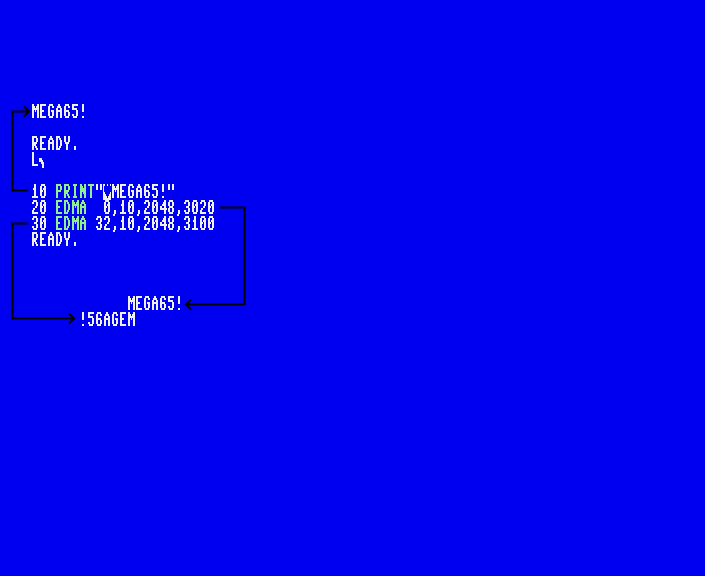
\includegraphics[width=\linewidth]{images/basic-example-edma.png}\end{center}
\end{description}

% **
% EL
% **

\newpage
\subsection{EL}
\index{BASIC 65 System Variables!EL}
\begin{description}[leftmargin=2cm,style=nextline]
\item [Token:]    N/A

\item [Format:]   {\bf EL}

\item [Usage:]    The line number where the most recent BASIC error occurred, or the value -1 if there was no error.

\item [Remarks:]  {\bf EL} is a reserved system variable.

                  This variable is typically used in a {\bf TRAP} routine, where the error line is taken from {\bf EL}.

\item [Example:]  Using {\bf EL}

\begin{tcolorbox}[colback=black,coltext=white]
\verbatimfont{\codefont}
\begin{verbatim}
 10 TRAP 100
 20 PRINT SQR(-1)                           : REM PROVOKE ERROR
 30 PRINT "AT LINE 30"                      : REM HERE TO RESUME
 40 END
100 IF ER > 0 THEN PRINT ERR$(ER); " ERROR"
110 PRINT " IN LINE"; EL
120 RESUME NEXT                             : REM RESUME AFTER ERROR
\end{verbatim}
\end{tcolorbox}
\end{description}

% *******
% ELLIPSE
% *******

\newpage
\subsection{ELLIPSE}
\index{BASIC 65 Commands!ELLIPSE}
\begin{description}[leftmargin=2cm,style=nextline]
\item [Token:]    \$FE \$30

\item [Format:]   {\bf ELLIPSE} xc{\bf,} yc{\bf,} xr{\bf,} yr[{\bf,} flags {\bf,} start{\bf,} stop]

\item [Usage:]    Bitmap graphics: draws an ellipse.

                  {\bf xc} the x coordinate of the centre in pixels.

                  {\bf yc} the y coordinate of the centre in pixels.

                  {\bf xr} the x radius of the ellipse in pixels.

                  {\bf yr} the y radius of the ellipse in pixels.

                  {\bf flags} controls the filling, arcs and orientation of the zero radian (combs flag named after {\bf retroCombs}). Default setting (zero) is: Don't fill, draw legs, start drawing at 3 'o clock.

                  {\setlength{\tabcolsep}{1.5mm}
                  \begin{tabular}{|l|l|l|l|}
                  \hline
                  {\bf Bit}  & {\bf Name} & {\bf Value} & {\bf Action if set} \\
                  \hline
                  0 & fill  & 1  & Fill ellipse or arc with the current pen colour \\
                  1 & legs  & 2  & Suppress drawing of the legs of an arc \\
                  2 & combs & 4  & Drawing (0 degree) starts at 12 'o clock \\
                  \hline
                  \end{tabular}
                  }

                  The units for the start- and stop-angle are degrees in the range of 0 to 360. The 0 radian starts at 3 o' clock and moves clockwise. The combs-flag shifts the 0 radian and the start position to the 12 'o clock position.

                  {\bf start} start angle for drawing an elliptic arc.

                  {\bf stop} stop angle for drawing an elliptic arc.

\item [Remarks:]  {\bf ELLIPSE} is used to draw ellipses on screens at various resolutions. If a full ellipse is to be drawn, start and stop should be either omissed or set both to zero (not 0 and 360). Drawing and filling of full ellipses is much faster, than using elliptic arcs.

\item [Example:]  Using {\bf ELLIPSE}

\begin{tcolorbox}[colback=black,coltext=white]
\verbatimfont{\codefont}
\begin{verbatim}
100 S% = 2 : D% = 3 : W% = 320 * S% : H% = 200 * S%         : REM SCREEN SETTINGS
110 CX% = W% / 2 : CY% = H% / 2                             : REM CENTRE AND RADII
120 RX% = W% / 2 : RY% = H% / 2
130 SCREEN W%, H%, D%                                       : REM OPEN SCREEN
140 ELLIPSE CX%, CY%, CX% - 4, CY% - 4
150 PEN 2 : CIRCLE CX%, CY%, RY% - 4, 2
160 PEN 3 : CIRCLE CX%, CY%, RY% - 14, 2
170 PEN 4 : CIRCLE CX%, CY%, RY% - 24, 0, 135, 45
180 PEN 5 : ELLIPSE CX%, CY% / 2, RX% / 4, RY% / 4, 1
190 PEN 6 : CIRCLE 120 * S%, CY%, 40, 1, 45, 315
200 PEN 7 : CIRCLE 200 * S%, CY%, 40, 1, 225, 135
210 PEN 0 : CHAR 34, CY% / 2 - 8, 2, 2, 2, "MEGA65", $3D000
220 GETKEY A&                                               : REM WAIT FOR ANY KEY
230 SCREEN CLOSE                                            : REM CLOSE GRAPHICS SCREEN
\end{verbatim}
\end{tcolorbox}

\item \begin{center}\includegraphics[width=0.7\linewidth]{images/ellipse.png}\end{center}
\end{description}

% ****
% ELSE
% ****

\newpage
\subsection{ELSE}
\index{BASIC 65 Commands!ELSE}
\begin{description}[leftmargin=2cm,style=nextline]
\item [Token:]    \$D5

\item [Format:]   {\bf IF} expression {\bf THEN} true clause [{\bf ELSE} false clause]

\item [Usage:]    {\bf ELSE} is an optional part of an {\bf IF} statement.

                  {\bf expression} logical or numeric expression. A numeric expression is evaluated as {\bf FALSE} if the value is zero and {\bf TRUE} for any non-zero value.

                  {\bf true clause} one or more statements starting directly after {\bf THEN} on the same line. A line number after {\bf THEN} performs a {\bf GOTO} to that line instead.

                  {\bf false clause} one or more statements starting directly after {\bf ELSE} on the same line. A line number after {\bf ELSE} performs a {\bf GOTO} to that line instead.

\item [Remarks:]  There must be a colon before {\bf ELSE}. There cannot be a colon or end-of-line after {\bf ELSE}.

                  The standard {\bf IF} ... {\bf THEN} ... {\bf ELSE} structure is restricted to a single line, but the {\bf true clause} and {\bf false clause} may be expanded to several lines using a compound statement surrounded with {\bf BEGIN} ... {\bf BEND}.

                  When the {\bf true clause} does not use {\bf BEGIN} ... {\bf BEND}, {\bf ELSE} must be on the same line as {\bf IF}.

\item [Examples:] Using {\bf ELSE}

\begin{tcolorbox}[colback=black,coltext=white]
\verbatimfont{\codefont}
\begin{verbatim}
100 REM ELSE
110 RED$ = CHR$(28) : BLACK$ = CHR$(144) : WHITE$ = CHR$(5)
120 INPUT "ENTER A NUMBER"; V
130 IF V < 0 THEN PRINT RED$; : ELSE PRINT BLACK$;
140 PRINT V                                                 : REM PRINT NEGATIVE NUMBERS IN RED
150 PRINT WHITE$
160 INPUT "END PROGRAM (Y/N)"; A$
170 IF A$ = "Y" THEN END
180 IF A$ = "N" THEN 120 : ELSE 160
\end{verbatim}
\end{tcolorbox}

                  Using {\bf ELSE} with {\bf BEGIN} ... {\bf BEND}

\begin{tcolorbox}[colback=black,coltext=white]
\verbatimfont{\codefont}
\begin{verbatim}
100 A=0 : GOSUB 200
110 A=1 : GOSUB 200
120 END
200 IF A=0 THEN BEGIN
210 PRINT "HELLO"
220 BEND : ELSE BEGIN
230 PRINT "GOODBYE"
240 BEND
250 RETURN
\end{verbatim}
\end{tcolorbox}
\end{description}

% ***
% END
% ***

\newpage
\subsection{END}
\index{BASIC 65 Commands!END}
\begin{description}[leftmargin=2cm,style=nextline]
\item [Token:]    \$80

\item [Format:]   {\bf END}

\item [Usage:]    Ends the execution of the BASIC program.

                  The \screentext{READY} prompt appears and the computer goes into direct mode waiting for keyboard input.

\item [Remarks:]  {\bf END} does \emph{not} clear channels \emph{nor} close files.

                  Variable definitions are still valid after {\bf END}.
                  
                  The program may be continued with the {\bf CONT} statement. After executing the last line of a program, {\bf END} is executed automatically.

\item [Example:]  Using {\bf END}

\begin{tcolorbox}[colback=black,coltext=white]
\verbatimfont{\codefont}
\begin{verbatim}
10 IF V < 0 THEN END : REM NEGATIVE NUMBERS END THE PROGRAM
20 PRINT V
\end{verbatim}
\end{tcolorbox}
\end{description}

% ********
% ENVELOPE
% ********

\newpage
\subsection{ENVELOPE}
\index{BASIC 65 Commands!ENVELOPE}
\begin{description}[leftmargin=2cm,style=nextline]
\item [Token:]    \$FE \$0A

\item [Format:]   {\bf ENVELOPE} n [\{{\bf,} attack{\bf,} decay{\bf,} sustain{\bf,} release{\bf,} waveform{\bf,} pw\}]

\item [Usage:]    Sets the parameters for the synthesis of a musical instrument for use with {\bf PLAY}.
                  
                  {\bf n} envelope slot (0 -- 9).

                  {\bf attack} attack rate (0 -- 15).

                  {\bf decay} decay rate (0 -- 15).

                  {\bf sustain} sustain rate (0 -- 15).

                  {\bf release} release rate (0 -- 15).

                  {\bf waveform} 0: triangle, 1: sawtooth, 2: square/pulse, 3: noise, or 4: ring modulation.

                  {\bf pw} pulse width (0 -- 4095) for waveform.

                  \label{envelopetable}
                  There are 10 slots for storing instrument parameters, preset with the following default values:

                  \begin{center}
                  {\setlength{\tabcolsep}{1mm}
                  \begin{tabular}{*{6}{|R{5mm}}|R{9mm}|l|}
                  \hline
                  {\bf n} & {\bf A} & {\bf D} & {\bf S} & {\bf R} & {\bf WF} & {\bf PW} & {\bf Instrument} \\
                  \hline
                  0 & 0 &  9 &  0 &  0 &  2 &  1536  &     Piano \\
                  1 & 12&  0 & 12 &  0 &  1 &        &     Accordion \\
                  2 & 0 &  0 & 15 &  0 &  0 &        &     Calliope \\
                  3 & 0 &  5 &  5 &  0 &  3 &        &     Drum \\
                  4 & 9 &  4 &  4 &  0 &  0 &        &     Flute \\
                  5 & 0 &  9 &  2 &  1 &  1 &        &     Guitar \\
                  6 & 0 &  9 &  0 &  0 &  2 &  512   &     Harpsichord \\
                  7 & 0 &  9 &  9 &  0 &  2 &  2048  &     Organ \\
                  8 & 8 &  9 &  4 &  1 &  2 &  512   &     Trumpet \\
                  9 & 0 &  9 &  0 &  0 &  0 &        &     Xylophone \\
                  \hline
                  \end{tabular}
                  }
                  \end{center}

\item [Example:]  Using {\bf ENVELOPE}

\begin{tcolorbox}[colback=black,coltext=white]
\verbatimfont{\codefont}
\begin{verbatim}
10 ENVELOPE 9, 10, 5, 10, 5, 2, 4000
20 VOL 9, 9
30 TEMPO 30
40 PLAY "T9O4Q CDEFGAB U3T8 CDEFGAB L", "T5O3Q H CGEQG T7 HCGEQG L"
\end{verbatim}
\end{tcolorbox}
\end{description}

% **
% ER
% **

\newpage
\subsection{ER}
\index{BASIC 65 System Variables!ER}
\begin{description}[leftmargin=2cm,style=nextline]
\item [Token:]    N/A

\item [Format:]   {\bf ER}

\item [Usage:]    The number of the most recent BASIC error that has occurred, or -1 if there was no error.

\item [Remarks:]  {\bf ER} is a reserved system variable.

                  This variable is typically used in a {\bf TRAP} routine, where the error number is taken from {\bf ER}.

\item [Example:]  Using {\bf ER}

\begin{tcolorbox}[colback=black,coltext=white]
\verbatimfont{\codefont}
\begin{verbatim}
10 TRAP 100
20 PRINT SQR(-1)         : REM PROVOKE ERROR
30 PRINT "AT LINE 30"    : REM HERE TO RESUME
40 END
100 IF ER > 0 THEN PRINT ERR$(ER); " ERROR";
110 PRINT " IN LINE"; EL
120 RESUME NEXT          : REM RESUME AFTER ERROR
\end{verbatim}
\end{tcolorbox}
\end{description}

% *****
% ERASE
% *****

\newpage
\subsection{ERASE}
\index{BASIC 65 Commands!ERASE}
\label{BASIC 65 Commands!ERASE}
\begin{description}[leftmargin=2cm,style=nextline]
\item [Token:]    \$FE \$2A

\item [Format:]   {\bf ERASE} filename [{\bf,D} drive] [{\bf,U} unit] [{\bf,R}]

\item [Usage:]    Erases (deletes) a disk file.

                  \filenamedefinition

                  \drivedefinition

                  \unitdefinition

                  {\bf R} will recover a previously erased file. This will only work if there were no write operations between erasing and recovery, which may have altered the contents of the disk.

\item [Remarks:]  {\bf ERASE} is a synonym of {\bf SCRATCH} and {\bf DELETE}.

                  In direct mode, the success and the number of erased files is printed. The second to last number from the message contains the number of successfully erased files.

\item [Examples:] Using {\bf ERASE}

\begin{tcolorbox}[colback=black,coltext=white]
\verbatimfont{\codefont}
\begin{verbatim}
ERASE "DRM", U9           : REM ERASE THE FILE "DRM" ON UNIT 9
01, FILES SCRATCHED,01,00

ERASE "OLD*"              : REM ERASE ALL FILES BEGINNING WITH "OLD"
01, FILES SCRATCHED,04,00

ERASE "R*=PRG"            : REM ERASE PROGRAM FILES STARTING WITH "R"
01, FILES SCRATCHED,09,00
\end{verbatim}
\end{tcolorbox}
\end{description}

% *****
% ERR\$
% *****

\newpage
\subsection{ERR\$}
\index{BASIC 65 Functions!ERR\$}
\begin{description}[leftmargin=2cm,style=nextline]
\item [Token:]    \$D3

\item [Format:]   {\bf ERR\$(}number{\bf)}

\item [Returns:]  The string description of a given BASIC error number.

                  {\bf number} BASIC error number (range  1 -- 44).

                  This function is typically used in a {\bf TRAP} routine, where the error number is taken from the reserved variable {\bf ER}.

\item [Remarks:]  A BASIC error number out of range (1 -- 44) will produce an \screentext{OK}.

\item [Examples:] Using {\bf ERR\$}

\begin{tcolorbox}[colback=black,coltext=white]
\verbatimfont{\codefont}
\begin{verbatim}
10 TRAP 100
20 PRINT SQR(-1)         : REM PROVOKE ERROR
30 PRINT "AT LINE 30"    : REM HERE TO RESUME
40 END
100 IF ER > 0 THEN PRINT ERR$(ER); " ERROR";
110 PRINT " IN LINE"; EL
120 RESUME NEXT          : REM RESUME AFTER ERROR
\end{verbatim}
\end{tcolorbox}

                  Displaying all error numbers and their descriptions

\begin{tcolorbox}[colback=black,coltext=white]
\verbatimfont{\codefont}
\begin{verbatim}
100 SCNCLR
110 FOR N = 0 TO 255
120 PRINT USING "###"; N; ": "; ERR$(N)
130 IF MOD(N, 16) <> 15 THEN 160
140 PRINT "[ MORE ]"
150 GETKEY A$
160 NEXT N
170 PRINT "DONE"
\end{verbatim}
\end{tcolorbox}
\end{description}

% ****
% EXIT
% ****

\newpage
\subsection{EXIT}
\index{BASIC 65 Commands!EXIT}
\begin{description}[leftmargin=2cm,style=nextline]
\item [Token:]    \$ED

\item [Format:]   {\bf EXIT}

\item [Usage:]    Exits the current {\bf DO} ... {\bf LOOP} and continues execution at the first statement after {\bf LOOP}.

\item [Remarks:]  In nested loops, {\bf EXIT} exits only the current loop, and continues execution in the outer loop (if there is one).

\item [Example:]  Using {\bf EXIT}

\begin{tcolorbox}[colback=black,coltext=white]
\verbatimfont{\codefont}
\begin{verbatim}
1 REM EXIT
10 OPEN 2, 8, 0, "$"           : REM OPEN CATALOG
15 IF DS THEN PRINT DS$ : STOP : REM CANT READ
20 GET#2, D$, D$               : REM DISCARD LOAD ADDRESS
25 DO                          : REM LINE LOOP
30   GET#2, D$, D$             : REM DISCARD LINE LINK
35   IF ST THEN EXIT           : REM END-OF-FILE
40   GET#2, LO, HI             : REM FILE SIZE BYTES
45   S = LO + 256 * HI         : REM FILE SIZE
50   LINE INPUT#2, F$          : REM FILE NAME
55   PRINT S; F$               : REM PRINT FILE ENTRY
60 LOOP
65 CLOSE 2
\end{verbatim}
\end{tcolorbox}
\end{description}

% ***
% EXP
% ***

\newpage
\subsection{EXP}
\index{BASIC 65 Functions!EXP}
\begin{description}[leftmargin=2cm,style=nextline]
\item [Token:]    \$BD

\item [Format:]   {\bf EXP(}numeric expression{\bf)}

\item [Returns:]  The value of the mathematical constant Euler's number (2.71828183) raised to the power of the argument.

\item [Remarks:]  An argument greater than 88 produces an Overflow error.

\item [Examples:] Using {\bf EXP}

\begin{tcolorbox}[colback=black,coltext=white]
\verbatimfont{\codefont}
\begin{verbatim}
PRINT EXP(1)
 2.7182818

PRINT EXP(0)
 1

PRINT EXP(LOG(2))
 2
\end{verbatim}
\end{tcolorbox}
\end{description}

% ****
% FAST
% ****

\newpage
\subsection{FAST}
\index{BASIC 65 Commands!FAST}
\begin{description}[leftmargin=2cm,style=nextline]
\item [Token:]    \$FE \$25

\item [Format:]   {\bf FAST} [speed]

\item [Usage:]    Sets CPU clock speed to 1 MHz, 3.5 MHz or 40 MHz.

                  {\bf speed} CPU clock speed where:

                  \begin{itemize}
                     \item 1: Sets CPU to 1 MHz.
                     \item 3: Sets CPU to 3.5 MHz.
                     \item Anything other than {\bf 1} or {\bf 3} sets the CPU to 40 MHz.
                  \end{itemize}

\item [Remarks:]  Although it's possible to call {\bf FAST} with any real number, the precision part (the decimal point and any digits after it), will be ignored.

                  {\bf FAST} is a synonym of {\bf SPEED}.

                  {\bf FAST} has no effect if \screentext{POKE 0, 65} has previously been used to set the CPU to 40 MHz.

\item [Examples:] Using {\bf FAST}

\begin{tcolorbox}[colback=black,coltext=white]
\verbatimfont{\codefont}
\begin{verbatim}
FAST     : REM SET SPEED TO MAXIMUM (40 MHZ)

FAST 1   : REM SET SPEED TO 1 MHZ

FAST 3   : REM SET SPEED TO 3.5 MHZ

FAST 3.5 : REM SET SPEED TO 3.5 MHZ
\end{verbatim}
\end{tcolorbox}
\end{description}

% ******
% FGOSUB
% ******

\newpage
\subsection{FGOSUB}
\index{BASIC 65 Commands!FGOSUB}
\begin{description}[leftmargin=2cm,style=nextline]
\item [Token:]    \$FE \$48

\item [Format:]   {\bf FGOSUB} numeric expression

\item [Usage:]    Evaluates the given numeric expression, then call {\bf GOSUB}s the subroutine at the resulting line number.

\item [Remarks:]  Take care when using {\bf RENUMBER} to change the line numbers of your program that any {\bf FGOSUB} statements still use the intended numbers. If the line number doesn't exist, FGOSUB throws an Undefined Statement error.

\item [Example:]  Using {\bf FGOSUB}

\begin{tcolorbox}[colback=black,coltext=white]
\verbatimfont{\codefont}
\begin{verbatim}
 10 INPUT "WHICH SUBROUTINE TO EXECUTE 100, 200, 300"; LI
 20 FGOSUB LI                    : REM HOPEFULLY THIS LINE # EXISTS
 30 GOTO 10                      : REM REPEAT
100 PRINT "AT LINE 100" : RETURN
200 PRINT "AT LINE 200" : RETURN
300 PRINT "AT LINE 300" : RETURN
\end{verbatim}
\end{tcolorbox}
\end{description}

% *****
% FGOTO
% *****

\newpage
\subsection{FGOTO}
\index{BASIC 65 Commands!FGOTO}
\begin{description}[leftmargin=2cm,style=nextline]
\item [Token:]    \$FE \$47
\item [Format:]   {\bf FGOTO} numeric expression
\item [Usage:]    Evaluates the given numeric expression, then {\bf GOTO}s to the resulting line number.

\item [Remarks:]  Take care when using {\bf RENUMBER} to change the line numbers of your program that any {\bf FGOTO} statements still use the intended numbers. If the line number doesn't exist, an Undefined Statement error will occur.

\item [Example:]  Using {\bf FGOTO}

\begin{tcolorbox}[colback=black,coltext=white]
\verbatimfont{\codefont}
\begin{verbatim}
 10 INPUT "WHICH LINE # TO EXECUTE 100, 200, 300"; LI
 20 FGOTO LI            : REM HOPEFULLY THIS LINE # EXISTS
 30 END
100 PRINT "AT LINE 100" : END
200 PRINT "AT LINE 200" : END
300 PRINT "AT LINE 300" : END
\end{verbatim}
\end{tcolorbox}
\end{description}

% ******
% FILTER
% ******

\newpage
\subsection{FILTER}
\index{BASIC 65 Commands!FILTER}
\begin{description}[leftmargin=2cm,style=nextline]
\item [Token:]    \$FE \$03

\item [Format:]   {\bf FILTER} sid [\{{\bf,} freq{\bf,} lp{\bf,} bp{\bf,} hp{\bf,} res\}]

\item [Usage:]    Sets the parameters for a SID sound filter.

                  {\bf sid} 1: right SID, 2: left SID.

                  {\bf freq} filter cut off frequency (0 - 2047).

                  {\bf lp} low pass filter (0: off, 1: on).

                  {\bf bp} band pass filter (0: off, 1: on).

                  {\bf hp} high pass filter (0: off, 1: on).

                  {\bf resonance} resonance (0 - 15).

\item [Remarks:]  Missing parameters keep their current value. The effective filter is the sum of of all filter settings. This enables band reject and notch effects.

\item [Example:]  Using {\bf FILTER}

\begin{tcolorbox}[colback=black,coltext=white]
\verbatimfont{\codefont}
\begin{verbatim}
 10 PLAY "T7X1O3P9C"
 15 SLEEP 0.02
 20 PRINT "LOW PASS SWEEP"  : L = 1 : B = 0 : H = 0 : GOSUB 100
 30 PRINT "BAND PASS SWEEP" : L = 0 : B = 1 : H = 0 : GOSUB 100
 40 PRINT "HIGH PASS SWEEP" : L = 0 : B = 0 : H = 1 : GOSUB 100
 50 GOTO 20
100 REM *** SWEEP ***
110 FOR F = 50 TO 1950 STEP 50
120 IF F >= 1000 THEN FF = 2000 - F : ELSE FF = F
130 FILTER 1, FF, L, B, H, 15
140 PLAY "X1"
150 SLEEP 0.02
160 NEXT F
170 RETURN
\end{verbatim}
\end{tcolorbox}
\end{description}

% ****
% FIND
% ****

\newpage
\subsection{FIND}
\index{BASIC 65 Commands!FIND}
\begin{description}[leftmargin=2cm,style=nextline]
\item [Token:]    \$FE \$2B

\item [Format:]   {\bf FIND /}string{\bf/} [{\bf,} line range] \\
		            {\bf FIND "}string{\bf"} [{\bf,} line range]

\item [Usage:]    Searches the BASIC program that is currently in memory for all instances of a string.

                  It searches a given line range (if specified), otherwise the entire BASIC program is searched.

                  At each occurrence of the "string", the line is listed with the string highlighted.

                  \specialkey{NO\\SCROLL} can be used to pause the output.

\item [Remarks:]  Almost any character that is not part of the string, including letters and punctuation, can be used instead of the '/' (slash).

                  Using double quotes ({\bf "}) as a delimiter has a special effect: The search text is not tokenised. {\bf FIND "FOR"} will search for the three letters ``F,'' ``O,'', and ``R,'' not the BASIC keyword {\bf FOR}. Therefore, it can find the word {\bf FOR} in string constants or {\bf REM} statements, but not in program code.

                  On the other hand, {\bf FIND /FOR/} will find all occurrences of the BASIC keyword, but not the text "FOR" in strings.

                  Partial keywords cannot be searched. For example, {\bf FIND /LOO/} will not find the keyword {\bf LOOP}.

                  Due to how BASIC is parsed, finding the {\bf REM} and {\bf DATA} keywords requires using the colon as the delimiter: {\bf FIND :REM TODO:} This does not work with the {\bf CHANGE} command.

                  {\bf FIND} is an editor command that can only be used in direct mode.

\item [Example:]  Using {\bf FIND}

\item \begin{center}\includegraphics[width=0.8\linewidth]{images/find-example.png}\end{center}
\end{description}

% **
% FN
% **

\newpage
\subsection{FN}
\index{BASIC 65 Functions!FN}
\begin{description}[leftmargin=2cm,style=nextline]
\item [Token:]    \$A5

\item [Format:]   {\bf FN} name{\bf(}numeric expression{\bf)}

\item [Usage:]    {\bf FN} functions are user-defined functions, that accept a numeric expression as an argument and return a real value.
                  They must first be defined with {\bf DEF FN} before being used.

                  {\bf name} name of the function as previously defined by {\bf DEF FN}.

\item [Example:]  Using {\bf FN}

\begin{tcolorbox}[colback=black,coltext=white]
\verbatimfont{\codefont}
\begin{verbatim}
10 PD = ~ / 180
20 DEF FN CD(X) = COS(X * PD)     : REM COS FOR DEGREES
30 DEF FN SD(X) = SIN(X * PD)     : REM SIN FOR DEGREES
40 FOR D = 0 TO 360 STEP 90
50 PRINT USING "###"; D;
60 PRINT USING " ##.##"; FNCD(D);
70 PRINT USING " ##.##"; FNSD(D)
80 NEXT D

RUN
  0  1.00  0.00
 90  0.00  1.00
180 -1.00  0.00
270  0.00 -1.00
360  1.00  0.00
\end{verbatim}
\end{tcolorbox}
\end{description}

% ****
% FONT
% ****

\newpage
\subsection{FONT}
\index{BASIC 65 Commands!FONT}
\begin{description}[leftmargin=2cm,style=nextline]
\item [Token:]    \$FE \$46
\item [Format:]   {\bf FONT} <{\bf A} | {\bf B} | {\bf C}>
\item [Usage:]    Updates all characters to the given built-in font.

                  {\bf FONT A} is the PETSCII font with several lowercase characters replaced with ASCII punctuation.

                  {\bf FONT B} is an alternate appearance of {\bf FONT A}.

                  {\bf FONT C} is the PETSCII font. This is the default when the MEGA65 is first switched on.

                  This resets any changes made by the {\bf CHARDEF} command.

                  The ASCII symbols of fonts {\bf A} and {\bf B} are typed by pressing the keys in the table below, some of which also require the holding down of the \megasymbolkey key. The codes for uppercase and lowercase are swapped compared to ASCII.

                  \begin{center}
                  {\setlength{\tabcolsep}{1mm}
                  \begin{tabular}{|C{1cm}|L{4.5cm}|C{1.4cm}|L{2.3cm}|}
                  \hline
                  {\bf Code}  & {\bf Key} & {\bf PETSCII} & {\bf ASCII}  \\
                  \hline
                     \$5C & Pound      & {\codefont \textbackslash}   & {\tt \textbackslash} (backslash) \\
                     \$5E & Up Arrow (next to RESTORE)  & {\codefont \textasciicircum} & {\tt \textasciicircum} (caret) \\
                     \$5F & Left Arrow (next to 1)      & {\codefont \_}               & {\tt \_} (underscore)   \\
                     \$7B & MEGA + Colon                & {\codefont ě }               & {\tt \{} (open brace)   \\
                     \$7C & MEGA + Dot                  & {\codefont Ĝ }               & {\tt |} (pipe)  \\
                     \$7D & MEGA + Semicolon            & {\codefont ĝ }               & {\tt \}} (close brace)  \\
                     \$7E & MEGA + Comma                & {\codefont \textasciitilde}  & {\tt \textasciitilde} (tilde)   \\
                  \hline
                  \end{tabular}
                  }
                  \end{center}

\item [Remarks:]  The additional ASCII characters provided by {\bf FONT A} and {\bf B} are only available while using the lowercase character set.

\item [Examples:] Using {\bf FONT}

\begin{tcolorbox}[colback=black,coltext=white]
%\verbatimfont{\codefont}
\begin{verbatim}
FONT A : REM ASCII - ENABLE {|}_~^
FONT B : REM SIMILAR TO A, WITH A SERIF FONT
FONT C : REM COMMODORE FONT (DEFAULT)
\end{verbatim}
\end{tcolorbox}
\end{description}

% ***
% FOR
% ***

\newpage
\subsection{FOR}
\index{BASIC 65 Commands!FOR}
\begin{description}[leftmargin=2cm,style=nextline]
\item [Token:]    \$81

\item [Format:]   {\bf FOR} index {\bf=} start {\bf TO} end	[{\bf STEP} step] ... {\bf NEXT} [index]

\item [Usage:]    {\bf FOR} statements start a BASIC loop with an index variable.

                  {\bf index} may be incremented or decremented by a constant value on each iteration. The default is to increment the variable by 1. The index variable must be a real variable.

                  {\bf start} is used to initialise the index.

                  {\bf end} is checked at the end of an iteration, and determines whether another iteration will be performed, or if the loop will exit.

                  {\bf step} defines the change applied to the index variable at the end of an iteration. Positive step values increment it, while negative values decrement it. It defaults to 1.0 if not specified.

\item [Remarks:]  For positive increments {\bf end} must be greater than or equal to {\bf start}, whereas for negative increments {\bf end} must be less than or equal to {\bf start}.

                  It is bad programming practice to change the value of the {\bf index} variable inside the loop or to jump into or out of a loop body with {\bf GOTO}.

\item [Examples:] Using {\bf FOR}

\begin{tcolorbox}[colback=black,coltext=white]
\verbatimfont{\codefont}
\begin{verbatim}
10 FOR D = 0 TO 360 STEP 30
20 R = D * ~ / 180
30 PRINT D; R; SIN(R); COS(R); TAN(R)
40 NEXT D

10 DIM M(20, 20)
20 FOR I = 0 TO 20
30 FOR J = I TO 20
40 M(I, J) = I + 100 * J
50 NEXT J, I
\end{verbatim}
\end{tcolorbox}
\end{description}

% **********
% FOREGROUND
% **********

\newpage
\subsection{FOREGROUND}
\index{BASIC 65 Commands!FOREGROUND}
\begin{description}[leftmargin=2cm,style=nextline]
\item [Token:]    \$FE \$39

\item [Format:]   {\bf FOREGROUND} colour

\item [Usage:]    Sets the foreground text colour for subsequent {\bf PRINT} commands.

                  {\bf colour} palette entry number, in the range 0 -- 31.

                  See appendix \vref{appendix:colourtable} for the list of colours in the default system palette.

\item [Remarks:]  This is another name for {\bf COLOR}.

\item [Example:]  Using {\bf FOREGROUND}

\item \begin{center}\includegraphics[width=0.7\linewidth]{images/foreground-example.png}\end{center}

\end{description}

% ******
% FORMAT
% ******

\newpage
\subsection{FORMAT}
\index{BASIC 65 Commands!FORMAT}
\begin{description}[leftmargin=2cm,style=nextline]
\item [Token:]    \$FE \$37

\item [Format:]   {\bf FORMAT} diskname [{\bf,I} id] [{\bf,D} drive] [{\bf,U} unit]

\item [Usage:]    Formats a disk. \underline{NOTE}: {\em This erases all data on the disk.}

                  {\bf I} disk ID. The maximum length is 2 characters.

                  {\bf diskname} is either a quoted string, e.g. \screentext{"DATA"} or a string expression in brackets, e.g. \screentext{(DN\$)}. The maximum length of is 16 characters.

                  \drivedefinition

                  \unitdefinition

\item [Remarks:]  {\bf FORMAT} is another name for the {\bf HEADER} command.

                  For new floppy disks which have not already been formatted in MEGA65 (1581) format, it is necessary to specify the disk ID with the {\bf I} parameter. This switches the format command to low level format, which writes sector IDs and erases all contents. This takes some time, as every block on the floppy disk will be written.

                  If the {\bf I} parameter is omitted, a quick format will be performed. This is only possible if the disk has already been formatted as a MEGA65 or 1581 floppy disk. A quick format writes the new disk name and clears the block allocation map, marking all blocks as free. The disk ID is not changed, and blocks are not overwritten, so contents may be recovered with {\bf ERASE R}. You can read more about {\bf ERASE} on page \pageref{BASIC 65 Commands!ERASE}.

\item [Examples:] Using {\bf FORMAT}

\begin{tcolorbox}[colback=black,coltext=white]
\verbatimfont{\codefont}
\begin{verbatim}
FORMAT "ADVENTURE", IDK   : REM A FULL DISK FORMAT WITH NAME "ADVENTURE" AND ID "DK"

FORMAT "ZORK-I", U9       : REM QUICK FORMAT DISK IN UNIT 9 WITH NAME "ZORK-I"

FORMAT "DUNGEON", D1, U10 : REM QUICK FORMAT DISK IN DRIVE 1 UNIT 10 WITH NAME "DUNGEON"
\end{verbatim}
\end{tcolorbox}
\end{description}

% ***
% FRE
% ***

\newpage
\subsection{FRE}
\index{BASIC 65 Functions!FRE}
\begin{description}[leftmargin=2cm,style=nextline]
\item [Token:]    \$B8
\item [Format:]   {\bf FRE(}bank{\bf)}
\item [Returns:]  The number of free bytes for banks 0 or 1, or the ROM version if the argument is negative.

                  {\bf FRE(0)} returns the number of free bytes in bank 0, which is used for BASIC program source.

                  {\bf FRE(1)} returns the number of free bytes in bank 1, which is the bank for BASIC variables, arrays and strings. {\bf FRE(1)} also triggers ``garbage collection'', which is a process that collects strings in use at the top of the bank, thereby defragmenting string memory.

                  {\bf FRE(-1)} returns the ROM version, a six-digit number on the form \texttt{92XXXX}.

\item [Example:]  Using {\bf FRE}

\begin{tcolorbox}[colback=black,coltext=white]
\verbatimfont{\codefont}
\begin{verbatim}
10 PM = FRE(0)
20 VM = FRE(1)
30 RV = FRE(-1)
40 PRINT PM; " BYTES FREE FOR PROGRAM"
50 PRINT VM; " BYTES FREE FOR VARIABLES"
60 PRINT RV; " ROM VERSION"
\end{verbatim}
\end{tcolorbox}
\end{description}

% *****
% FREAD
% *****

\newpage
\subsection{FREAD}
\index{BASIC 65 Commands!FREAD}
\begin{description}[leftmargin=2cm,style=nextline]
\item [Token:]    \$FE \$1C
\item [Format:]   {\bf FREAD\#} channel{\bf,} pointer{\bf,} size
\item [Usage:]    Reads {\bf size} bytes from {\bf channel} to memory starting at the 32-bit address {\bf pointer}.

                  {\bf channel} number, which was given to a previous call to commands such as {\bf DOPEN}, or {\bf OPEN}

                  {\bf FREAD} can be used to read data from disk directly into a variable. It is recommended to use the {\bf POINTER} statement for the pointer argument, and to compute the size parameter by multiplying the number of elements with the item size.

                  \begin{center}
                  \label{freadtable}
                  \setlength{\tabcolsep}{1mm}
                  \begin{tabular}{|l|c|}
                  \hline
                  {\bf Type}     & {\bf Item Size} \\
                  \hline
                  Byte     Array &  1  \\
                  Integer  Array &  2  \\
                  Real     Array &  5  \\
                  \hline
                  \end{tabular}
                  \end{center}

\item [Remarks:]  Keep in mind that the {\bf POINTER} function with a string argument does {\em not} return the string address, but the string descriptor. It is not recommended to use {\bf FREAD} for strings or string arrays unless you are fully aware on how to handle the string storage internals.

                  To read into an array, ensure that you always specify an array index so that {\bf POINTER} returns the address of an element. The start address of array \screentext{XY()} is \screentext{POINTER(XY(0))}. \screentext{POINTER(XY)} returns the address of the scalar variable \screentext{XY}

\item [Example:]  Using {\bf FREAD}

\begin{tcolorbox}[colback=black,coltext=white]
\verbatimfont{\codefont}
\begin{verbatim}
100 N = 23
110 DIM B&(N), C&(N)
120 DOPEN#2, "TEXT"
130 FREAD#2, POINTER(B&(0)), N
140 DCLOSE#2
150 FOR I = 0 TO N - 1 : PRINT CHR$(B&(I)); : NEXT
160 FOR I = 0 TO N - 1 : C&(I) = B&(N - 1 - I) : NEXT
170 DOPEN#2, "REVERS,W"
180 FWRITE#2, POINTER(C&(0)), N
190 DCLOSE#2
\end{verbatim}
\end{tcolorbox}
\end{description}

% *******
% FREEZER
% *******

\newpage
\subsection{FREEZER}
\index{BASIC 65 Commands!FREEZER}
\begin{description}[leftmargin=2cm,style=nextline]
\item [Token:]    \$FE \$4A

\item [Format:]   {\bf FREEZER}

\item [Usage:]    Invokes the Freezer menu.

\item [Remarks:]  Entering the {\bf FREEZER} command is an alternative to holding and releasing the \widekey{RESTORE} key.

\item [Example:]  Using {\bf FREEZER}

\begin{tcolorbox}[colback=black,coltext=white]
\verbatimfont{\codefont}
\begin{verbatim}
FREEZER : REM CALL FREEZER MENU
\end{verbatim}
\end{tcolorbox}
\end{description}

% ******
% FWRITE
% ******

\newpage
\subsection{FWRITE}
\index{BASIC 65 Commands!FWRITE}
\begin{description}[leftmargin=2cm,style=nextline]
\item [Token:]    \$FE \$1E

\item [Format:]   {\bf FWRITE\#} channel{\bf,} pointer{\bf,} size

\item [Usage:]    Writes {\bf size} bytes to {\bf channel} from memory starting at the 32-bit address {\bf pointer}.

                  {\bf channel} number, which was given to a previous call to commands such as {\bf APPEND}, {\bf DOPEN}, or {\bf OPEN}.

                  {\bf FWRITE} can be used to write the value of a variable to a file.

                  It is recommended to use the {\bf POINTER} statement for the pointer argument and compute the size parameter by multiplying the number of elements with the item size.

                  Refer to the {\bf FREAD} item size table on page \pageref{freadtable} for the item sizes.

\item [Remarks:]  Keep in mind that the {\bf POINTER} function with a string argument does {\em not} return the string address, but the string descriptor. It is not recommended to use {\bf FWRITE} for strings or string arrays unless you are fully aware on how to handle the string storage internals.

                  To write an array, ensure that you always specify an array index so that {\bf POINTER} returns the address of an element. The start address of array \screentext{XY()} is \screentext{POINTER(XY(0))}. \screentext{POINTER(XY)} returns the address of the scalar variable \screentext{XY}.

\item [Example:]  Using {\bf FWRITE}

\begin{tcolorbox}[colback=black,coltext=white]
\verbatimfont{\codefont}
\begin{verbatim}
100 N = 23
110 DIM B&(N), C&(N)
120 DOPEN#2, "TEXT"
130 FREAD#2, POINTER(B&(0)), N
140 DCLOSE#2
150 FOR I = 0 TO N - 1 : PRINT CHR$(B&(I)); : NEXT
160 FOR I = 0 TO N - 1 : C&(I) = B&(N - 1 - I) : NEXT
170 DOPEN#2, "REVERS,W"
180 FWRITE#2, POINTER(C&(0)), N
190 DCLOSE#2
\end{verbatim}
\end{tcolorbox}
\end{description}

% *****
% GCOPY
% *****

\newpage
\subsection{GCOPY}
\index{BASIC 65 Commands!GCOPY}
\begin{description}[leftmargin=2cm,style=nextline]
\item [Token:]    \$FE \$32

\item [Format:]   {\bf GCOPY} x{\bf,} y{\bf,} width{\bf,} height

\item [Usage:]    Bitmap graphics: copies the content of the specified rectangle with upper left position {\bf x, y} and the {\bf width} and {\bf height} to a buffer.

                  The copied region can be inserted at any position with the command {\bf PASTE}.

\item [Remarks:]  The size of the rectangle is limited by the 1KB size of the buffer. The memory requirement for a region is width * height * number of bitplanes / 8. It must not equal or exceed 1024 bytes. For a 4-bitplane screen for example, a 45 x 45 region needs 1012.5 bytes.

\item [Example:]  Using {\bf GCOPY}

\begin{tcolorbox}[colback=black,coltext=white]
\verbatimfont{\codefont}
\begin{verbatim}
10 SCREEN 320, 200, 2
20 BOX 60, 60, 300, 180, 1 : REM DRAW A WHITE BOX
30 GCOPY 140, 80, 40, 40   : REM COPY A 40 * 40 REGION
40 PASTE 10, 10            : REM PASTE IT TO A NEW POSITION
50 GETKEY A$               : REM WAIT FOR A KEYPRESS
60 SCREEN CLOSE
\end{verbatim}
\end{tcolorbox}
\end{description}

% ***
% GET
% ***

\newpage
\subsection{GET}
\index{BASIC 65 Commands!GET}
\begin{description}[leftmargin=2cm,style=nextline]
\item [Token:]    \$A1

\item [Format:]   {\bf GET} variable

\item [Usage:]    Gets the next character, or byte value of the next character, from the keyboard queue.

                  If the {\bf variable} being set to the character is of type string and the queue is empty, an empty string is assigned to it, otherwise a one character string is created and assigned instead.
               
                  If the {\bf variable} is of type numeric, the byte value of the key is assigned to it, otherwise zero will be assigned if the queue is empty. {\bf GET} does not wait for keyboard input, so it's useful to check for key presses at regular intervals or in loops.

\item [Remarks:]  {\bf GETKEY} is similar, but waits until a key has been pressed.

\item [Example:]  Using {\bf GET}

\begin{tcolorbox}[colback=black,coltext=white]
\verbatimfont{\codefont}
\begin{verbatim}
10 DO : GET A$ : LOOP UNTIL A$ <> ""
20 IF A$ = "W" THEN PRINT "NORTH"  : REM GO NORTH
30 IF A$ = "A" THEN PRINT "WEST"   : REM GO WEST
40 IF A$ = "S" THEN PRINT "EAST"   : REM GO EAST
50 IF A$ = "Z" THEN PRINT "SOUTH"  : REM GO SOUTH
60 IF A$ = CHR$(13) THEN END       : REM EXIT
70 GOTO 10
\end{verbatim}
\end{tcolorbox}
\end{description}

% ****
% GET#
% ****

\newpage
\subsection{GET\#}
\index{BASIC 65 Commands!GET\#}
\begin{description}[leftmargin=2cm,style=nextline]
\item [Token:]    \$A1 '\#'

\item [Format:]   {\bf GET\#} channel{\bf,} variable [{\bf,} variable \dots]

\item [Usage:]    Reads a single byte from the channel argument and assigns single character strings to string variables, or an 8-bit binary value to numeric variables.

                  This is useful for reading characters (or bytes) from an input stream one byte at a time.

                  {\bf channel} number, which was given to a previous call to commands such as {\bf DOPEN}, or {\bf OPEN}.

\item [Remarks:]  All values from 0 to 255 are valid, so {\bf GET\#} can also be used to read binary data.

\item [Example:]  Using {\bf GET\#}

\begin{tcolorbox}[colback=black,coltext=white]
\verbatimfont{\codefont}
\begin{verbatim}
10 OPEN 2, 8, 0, "$"           : REM OPEN CATALOG
15 IF DS THEN PRINT DS$ : STOP : REM CANT READ
20 GET#2, D$, D$               : REM DISCARD LOAD ADDRESS
25 DO                          : REM LINE LOOP
30   GET#2, D$, D$             : REM DISCARD LINE LINK
35   IF ST THEN EXIT           : REM END-OF-FILE
40   GET#2, LO, HI             : REM FILE SIZE BYTES
45   S=LO+256*HI               : REM FILE SIZE
50   LINE INPUT#2, F$          : REM FILE NAME
55   PRINT S;F$                : REM PRINT FILE ENTRY
60 LOOP
65 CLOSE 2
\end{verbatim}
\end{tcolorbox}
\end{description}

% ******
% GETKEY
% ******

\newpage
\subsection{GETKEY}
\index{BASIC 65 Commands!GETKEY}
\begin{description}[leftmargin=2cm,style=nextline]
\item [Token:]    \$A1 (GET) \$F9 (KEY)

\item [Format:]   {\bf GETKEY} variable

\item [Usage:]    Gets the next character, or byte value of the next character, from the keyboard queue. If the queue is empty, the program will wait until a key has been pressed.

                  After a key has been pressed, the e {\bf variable} will be set and program execution will continue. When used with a string variable, a one character string is created and assigned. Otherwise if the variable is of type numeric, the byte value is assigned.

\item [Example:]  Using {\bf GETKEY}

\begin{tcolorbox}[colback=black,coltext=white]
\verbatimfont{\codefont}
\begin{verbatim}
10 GETKEY A$                      : REM WAIT AND GET CHARACTER
20 IF A$ = "W" THEN PRINT "NORTH" : REM GO NORTH
30 IF A$ = "A" THEN PRINT "WEST"  : REM GO WEST
40 IF A$ = "S" THEN PRINT "EAST"  : REM GO EAST
50 IF A$ = "Z" THEN PRINT "SOUTH" : REM GO SOUTH
60 IF A$ = CHR$(13) THEN END      : REM EXIT
70 GOTO 10
\end{verbatim}
\end{tcolorbox}
\end{description}

% ****
% GO64
% ****

\newpage
\subsection{GO64}
\index{BASIC 65 Commands!GO64}
\index{Commodore 64!GO64 mode}
\begin{description}[leftmargin=2cm,style=nextline]
\item [Token:]    \$CB (GO) \$36 \$34 ("64")

\item [Format:]   {\bf GO64}

\item [Usage:]    Switches the MEGA65 to C64-compatible mode.

                  If you're in direct mode, a security prompt \screentext{ARE YOU SURE?} is displayed, which must be responded with \texttt{Y} to continue.

                  You can switch back to MEGA65 mode with the command \screentext{SYS 58552}.

\item [Remarks:]  If you switch back to the MEGA65 using the \screentext{SYS 58552}, the switch will be immediate. No confirmation will be asked for.

\item [Example:]  Using {\bf GO64}

\begin{tcolorbox}[colback=black,coltext=white]
\verbatimfont{\codefont}
\begin{verbatim}
READY.
GO64
ARE YOU SURE? Y
\end{verbatim}
\end{tcolorbox}

                  Switch back to MEGA65

\begin{tcolorbox}[colback=black,coltext=white]
\verbatimfont{\codefont}
\begin{verbatim}
READY.
SYS 58552
\end{verbatim}
\end{tcolorbox}
\end{description}

% *****
% GOSUB
% *****

\newpage
\subsection{GOSUB}
\index{BASIC 65 Commands!GOSUB}
\begin{description}[leftmargin=2cm,style=nextline]
\item [Token:]    \$8D

\item [Format:]   {\bf GOSUB} line number

\item [Usage:]    {\bf GOSUB} (GOto SUBroutine) continues program execution at the given BASIC line number, saving the current BASIC program counter and line number on the run-time stack.
               
                  This enables the resumption of execution after the {\bf GOSUB} statement, once a {\bf RETURN} statement in the called subroutine is executed.
                  
                  Calls to subroutines via {\bf GOSUB} may be nested, but the subroutines must always end with {\bf RETURN}, otherwise a stack overflow may occur.

\item [Remarks:]  Unlike other programming languages, BASIC does not support arguments or local variables for subroutines. Programs can be optimised by grouping subroutines at the beginning of the program source. The {\bf GOSUB} calls will then have low line numbers with fewer digits to decode. The subroutines will also be found faster, since the search for subroutines often starts at the beginning of the program.

\item [Example:]  Using {\bf GOSUB}

\begin{tcolorbox}[colback=black,coltext=white]
\verbatimfont{\codefont}
\begin{verbatim}
 10 GOTO 100                                     : REM TO MAIN PROGRAM
 20 REM *** SUBROUTINE DISK STATUS CHECK ***
 30 DD = DS : IF DD THEN PRINT "DISK ERROR"; DS$
 40 RETURN
 50 REM *** SUBROUTINE PROMPT Y/N ***
 60 DO : INPUT "CONTINUE (Y/N)"; A$
 70 LOOP UNTIL A$ = "Y" OR A$ = "N"
 80 RETURN
 90 REM *** MAIN PROGRAM ***
100 DOPEN#2, "BIG DATA"
110 GOSUB 30 : IF DD THEN DCLOSE#2 : GOSUB 60    : REM ASK
120 IF A$ = "N" THEN END
130 GOTO 100                                     : REM RETRY
\end{verbatim}
\end{tcolorbox}
\end{description}

% ****
% GOTO
% ****

\newpage
\subsection{GOTO}
\index{BASIC 65 Commands!GOTO}
\begin{description}[leftmargin=2cm,style=nextline]
\item [Token:]    \$89 (GOTO) or \$CB \$A4 (GO TO)

\item [Format:]   {\bf GOTO} line \\
                  {\bf GO TO} line

\item [Usage:]    Continues program execution at the given BASIC line number.

\item [Remarks:]  If the target {\bf line} number is higher than the current line number, the search starts from the current line, proceeding to higher line numbers. If the target {\bf line} number is lower, the search starts at the first {\bf line} number of the program. It is possible to optimise the run-time speed of the program by grouping often used targets at the start (with lower line numbers).

                  {\bf GOTO} (written as a single word) executes faster than {\bf GO TO}.

\item [Example:]  Using {\bf GOTO}

\begin{tcolorbox}[colback=black,coltext=white]
\verbatimfont{\codefont}
\begin{verbatim}
 10 GOTO 100                                     : REM TO MAIN PROGRAM
 20 REM *** SUBROUTINE DISK STATUS CHECK ***
 30 DD = DS : IF DD THEN PRINT "DISK ERROR"; DS$
 40 RETURN
 50 REM *** SUBROUTINE PROMPT Y/N ***
 60 DO : INPUT "CONTINUE (Y/N)"; A$
 70 LOOP UNTIL A$ = "Y" OR A$ = "N"
 80 RETURN
 90 REM *** MAIN PROGRAM ***
100 DOPEN#2, "BIG DATA"
110 GOSUB 30 : IF DD THEN DCLOSE#2 : GOSUB 60    : REM ASK
120 IF A$ = "N" THEN END
130 GOTO 100                                     : REM RETRY
\end{verbatim}
\end{tcolorbox}
\end{description}

% *******
% GRAPHIC
% *******

\newpage
\subsection{GRAPHIC}
\index{BASIC 65 Commands!GRAPHIC}
\begin{description}[leftmargin=2cm,style=nextline]
\item [Token:]    \$DE

\item [Format:]   {\bf GRAPHIC CLR}

\item [Usage:]    Bitmap graphics: initialises the BASIC bitmap graphics system. It clears the graphics memory and screen, and sets all parameters of the graphics context to their default values.

                  Once the graphics system has been cleared, commands such as {\bf LINE}, {\bf PALETTE}, {\bf PEN}, {\bf SCNCLR}, and {\bf SCREEN} can be used to set graphics system parameters.

\item [Example:]  Using {\bf GRAPHIC}

\begin{tcolorbox}[colback=black,coltext=white]
\verbatimfont{\codefont}
\begin{verbatim}
110 GRAPHIC CLR            : REM INITIALISE
120 SCREEN DEF 1, 1, 1, 2  : REM 640 X 400 X 2
130 SCREEN OPEN 1          : REM OPEN IT
140 SCREEN SET 1, 1        : REM VIEW IT
150 PALETTE 1, 0, 0,  0, 0 : REM BLACK
160 PALETTE 1, 1, 0, 15, 0 : REM GREEN
170 SCNCLR 0               : REM FILL SCREEN WITH BLACK
180 PEN 0, 1               : REM SELECT PEN
190 LINE 50, 50, 590, 350  : REM DRAW LINE
200 GETKEY A$              : REM WAIT FOR KEYPRESS
210 SCREEN CLOSE 1         : REM CLOSE SCREEN AND RESTORE PALETTE
\end{verbatim}
\end{tcolorbox}
\end{description}

% ******
% HEADER
% ******

\newpage
\subsection{HEADER}
\index{BASIC 65 Commands!HEADER}
\begin{description}[leftmargin=2cm,style=nextline]
\item [Token:]    \$F1

\item [Format:]   {\bf HEADER} diskname [{\bf,I} id] [{\bf,D} drive] [{\bf,U} unit]

\item [Usage:]    Formats a disk. \underline{NOTE}: {\em This erases all data on the disk.}

                  {\bf I} disk ID. Maximum length is 2 characters.

                  {\bf diskname} is either a quoted string, e.g. \screentext{"DATA"} or a string expression in brackets, e.g. \screentext{(DN\$)} The maximum length is 16 characters.

                  \drivedefinition

                  \unitdefinition

\item [Remarks:]  {\bf HEADER} is another name for the {\bf FORMAT} command.

                  For new floppy disks which have not already been formatted in MEGA65 (1581) format, it is necessary to specify the disk ID with the {\bf I} parameter. This switches the format command to low level format, which writes sector IDs and erases all contents. This takes some time, as every block on the floppy disk will be written.

                  If the {\bf I} parameter is omitted, a quick format will be performed. This is only possible if the disk has already been formatted as a MEGA65 or 1581 floppy disk. A quick format writes the new disk name and clears the block allocation map, marking all blocks as free. The disk ID is not changed, and blocks are not overwritten, so contents may be recovered with {\bf ERASE R}. You can read more about {\bf ERASE} on page \pageref{BASIC 65 Commands!ERASE}.

\item [Examples:] Using {\bf HEADER}

\begin{tcolorbox}[colback=black,coltext=white]
\verbatimfont{\codefont}
\begin{verbatim}
HEADER "ADVENTURE", IDK   : REM A FULL DISK FORMAT WITH NAME "ADVENTURE" AND ID "DK"

HEADER "ZORK-I", U9       : REM QUICK FORMAT DISK IN UNIT 9 WITH NAME "ZORK-I"

HEADER "DUNGEON", D1, U10 : REM QUICK FORMAT DISK IN DRIVE 1 UNIT 10 WITH NAME "DUNGEON"
\end{verbatim}
\end{tcolorbox}
\end{description}

% ****
% HELP
% ****

\newpage
\subsection{HELP}
\index{BASIC 65 Commands!HELP}
\begin{description}[leftmargin=2cm,style=nextline]
\item [Token:]    \$EA

\item [Format:]   {\bf HELP}

\item [Usage:]    Displays information about where an error occurred in a BASIC program.

                  When the BASIC program stops due to an error, {\bf HELP} can be used to gain further information. The interpreted line is listed, with the erroneous statement highlighted or underlined.

\item [Remarks:]  Displays BASIC errors. For errors related to disk I/O, the disk status variable {\bf DS} or the disk status string {\bf DS\$} should be used instead.

\item [Example:]  Using {\bf HELP}

\begin{tcolorbox}[colback=black,coltext=white]
\verbatimfont{\codefont}
\begin{verbatim}
10 A = 1.E20
20 B = A + A : C = EXP(A) : PRINT A, B, C
RUN

?OVERFLOW ERROR IN 20
READY.
HELP

20 B = A + A : ţŝťŸŰňšʼn : PRINT A, B, C
\end{verbatim}
\end{tcolorbox}
\end{description}

% *****
% HEX\$
% *****

\newpage
\subsection{HEX\$}
\index{BASIC 65 Functions!HEX\$}
\begin{description}[leftmargin=2cm,style=nextline]
\item [Token:]    \$D2

\item [Format:]   {\bf HEX\$(}numeric expression{\bf)}

\item [Returns:]  A four or eight character hexadecimal representation of the argument.

                  The argument must be in the range of 0 -- 4294967295, corresponding to the hex numbers \$00000000-\$FFFFFFFF. If the argument is between 0 -- 65535, a four character string is returned. For all values above 65535, an eight character string is returned instead.

\item [Remarks:]  If real numbers are used as arguments, the fractional part will be ignored. In other words, real numbers will not be rounded.

\item [Examples:] Using {\bf HEX\$}

\begin{tcolorbox}[colback=black,coltext=white]
\verbatimfont{\codefont}
\begin{verbatim}
PRINT HEX$(10), HEX$(100), HEX$(1000.9)
000A      0064      03E8

PRINT HEX$(4294967295)
FFFFFFFF
\end{verbatim}
\end{tcolorbox}
\end{description}

% *********
% HIGHLIGHT
% *********

\newpage
\subsection{HIGHLIGHT}
\index{BASIC 65 Commands!HIGHLIGHT}
\begin{description}[leftmargin=2cm,style=nextline]
\item [Token:]    \$FE \$3D

\item [Format:]   {\bf HIGHLIGHT} colour [{\bf,} mode]

\item [Usage:]    Sets the colours used for code highlighting.

                  Different colours can be set for system messages, {\bf REM} statements and BASIC keywords.

                  {\bf colour} one of the first 16 colours in the current palette. See appendix \vref{appendix:colourtable} for the list of colours in the default system palette.

                  {\bf mode} indicates what the colour will be used for.
                  \begin{itemize}
                     \item 0: System messages (the default mode).
                     \item 1: {\bf REM} statements.
                     \item 2: BASIC keywords.
                  \end{itemize}

\item [Remarks:]  The system messages colour is used when displaying error messages, and in the output of {\bf CHANGE}, {\bf FIND}, and {\bf HELP}. The colours for {\bf REM} statements and BASIC keywords are used by {\bf LIST}.

\item [Example:]  Using {\bf HIGHLIGHT}

\item \begin{center}\includegraphics[width=0.8\linewidth]{images/highlight-example.png}\end{center}

\end{description}

% **
% IF
% **

\newpage
\subsection{IF}
\index{BASIC 65 Commands!IF}
\begin{description}[leftmargin=2cm,style=nextline]
\item [Token:]    \$8B

\item [Format:]   {\bf IF} expression {\bf THEN} true clause [{\bf ELSE} false clause]

\item [Usage:]    Starts a conditional execution statement.

                  {\bf expression} logical or numeric expression. A numeric expression is evaluated as {\bf FALSE} if the value is zero and {\bf TRUE} for any non-zero value.

                  {\bf true clause} one or more statements starting directly after {\bf THEN} on the same line. A line number after {\bf THEN} performs a {\bf GOTO} to that line instead.

                  {\bf false clause} one or more statements starting directly after {\bf ELSE} on the same line. A line number after {\bf ELSE} performs a {\bf GOTO} to that line instead.

\item [Remarks:]  The standard {\bf IF} ... {\bf THEN} ... {\bf ELSE} structure is restricted to a single line. However, the {\bf true clause} and {\bf false clause} may be expanded to several lines using a compound statement surrounded with {\bf BEGIN} ... {\bf BEND}.

\item [Example:]  Using {\bf IF}

\begin{tcolorbox}[colback=black,coltext=white]
\verbatimfont{\codefont}
\begin{verbatim}
10 RED$ = CHR$(28) : BLACK$ = CHR$(144) : WHITE$ = CHR$(5)
20 INPUT "ENTER A NUMBER"; V
30 IF V < 0 THEN PRINT RED$; : ELSE PRINT BLACK$;
40 PRINT V                                        : REM PRINT NEGATIVE NUMBERS IN RED
50 PRINT WHITE$
60 INPUT "END PROGRAM (Y/N)"; A$
70 IF A$ = "Y" THEN END
80 IF A$ = "N" THEN 20 : ELSE 60
\end{verbatim}
\end{tcolorbox}
\end{description}

% ******
% IMPORT
% ******

\newpage
\subsection{IMPORT}
\index{BASIC 65 Commands!IMPORT}
\begin{description}[leftmargin=2cm,style=nextline]
\item [Token:]    \$DD

\item [Format:]   {\bf IMPORT} filename [{\bf,D} drive] [{\bf,U} unit]

\item [Usage:]    Loads BASIC code in text format from a file of type {\bf SEQ} into memory reserved for BASIC programs.

                  \filenamedefinition

                  \drivedefinition

                  \unitdefinition

\item [Remarks:]  The program is loaded into BASIC memory and converted from text to the tokenised form of {\bf PRG} files. This enables loading of BASIC programs that were saved as plain text files as program listing.

                  After loading, the program is re-linked and ready to be {\bf RUN} or edited. It is possible to use {\bf IMPORT} for merging a program text file from disk to a program already in memory. Each line read from the file is processed in the same way, as if typed from the user with the screen editor.

                  There is no {\bf EXPORT} counterpart, because this function is already available. The sequence \screentext{DOPEN\#1,"LISTING",W:CMD 1:LIST:DCLOSE\#1} converts the program in memory to text and writes it to the file, that is named in the {\bf DOPEN} statement.

\item [Examples:] Using {\bf IMPORT}

\begin{tcolorbox}[colback=black,coltext=white]
\verbatimfont{\codefont}
\begin{verbatim}
IMPORT "APOCALYPSE"

IMPORT "MEGA TOOLS", U9

IMPORT (FI$), U(UN%)
\end{verbatim}
\end{tcolorbox}
\end{description}

% ****
% INFO
% ****

\newpage
\subsection{INFO}
\index{BASIC 65 Commands!INFO}
\begin{description}[leftmargin=2cm,style=nextline]
\item [Token:]    \$FE \$4D

\item [Format:]   {\bf INFO}

\item [Usage:]    Displays information about the runtime environment.

\item [Remarks:]  The {\bf INFO} command displays information about the BASIC runtime environment, including:

                  \begin{itemize}
                     \item The video mode (PAL, NTSC).
                     \item The version of the ROM.
                     \item The CPU speed.
                     \item The current {\bf MEM} setting.
                     \item Memory used and memory available for program text and variables.
                  \end{itemize}

\item [Example:]  Using {\bf INFO}

\begin{tcolorbox}[colback=black,coltext=white]
\verbatimfont{\codefont}
\begin{verbatim}
READY.
INFO

INFO: PAL     DATA BYTES  USED /  FREE
---------------------------------------
ROM-V   920408   PROGRAM:    7 / 55030
SPEED   40 MHZ   SCALARS:    0 /  1472
BANK4 --------   STRINGS:    0 / 54980
BANK5 --------   ARRAYS :    0 / 54980
\end{verbatim}
\end{tcolorbox}
\end{description}

% *****
% INPUT
% *****

\newpage
\subsection{INPUT}
\index{BASIC 65 Commands!INPUT}
\begin{description}[leftmargin=2cm,style=nextline]
\item [Token:]    \$85

\item [Format:]   {\bf INPUT} [prompt <{\bf,} | {\bf;}>] variable [{\bf,} variable ...]

\item [Usage:]    Prompts the user for keyboard input, printing an optional prompt string and question mark to the screen.

                  {\bf prompt} optional string expression to be printed as the prompt.

                  If the separator between {\bf prompt} and {\bf variable list} is a comma ({\bf ,}), the cursor is placed directly after the prompt. If the separator is a semicolon ({\bf ;}), a question mark and a space is added to the prompt instead.

                  {\bf variable list} one or more variables that receive the input.

                  The input will be processed after the user presses \specialkey{RETURN}.

\item [Remarks:]  The user must take care to enter the correct type of input, so it matches the {\bf variable list} types. Also, the number of input items must match the number of variables. A surplus of input items will be ignored, whereas too few input items trigger another request for input with the prompt \screentext{??}.
               
                  Typing non-numeric characters for integer or real variables will produce a Type Mismatch error.
                  
                  Strings for string variables must be in double quotes ({\bf "}) if they contain spaces or commas.
               
                  Many programs that need a safe input routine use {\bf LINE INPUT} and a custom parser, in order to avoid program errors by wrong user input.

\item [Example:]  Using {\bf INPUT}

\begin{tcolorbox}[colback=black,coltext=white]
\verbatimfont{\codefont}
\begin{verbatim}
 10 DIM N$(100), A%(100), S$(100)
 20 DO
 30 INPUT "NAME, AGE, GENDER";NA$, AG%, SE$
 40 IF NA$ = "" THEN 30
 50 IF NA$ = "END" THEN EXIT
 60 IF AG% < 18 OR AG% > 100 THEN PRINT "AGE?" : GOTO 30
 70 IF SE$ <> "M" AND SE$ <> "F" THEN PRINT "GENDER?" : GOTO 30
 80 REM CHECK OK. ENTER INTO ARRAY
 90 N$(N) = NA$ : A%(N) = AG% : S$(N) = SE$ : N = N + 1
100 LOOP UNTIL N = 100
110 PRINT "RECEIVED";N;" NAMES"
\end{verbatim}
\end{tcolorbox}
\end{description}

% *******
% INPUT\#
% *******

\newpage
\subsection{INPUT\#}
\index{BASIC 65 Commands!INPUT\#}
\begin{description}[leftmargin=2cm,style=nextline]
\item [Token:]    \$84

\item [Format:]   {\bf INPUT\#} channel{\bf,} variable [{\bf,} variable ...]

\item [Usage:]    Reads a record from an input device, e.g. a disk file, and assigns the data to the variables in the list.

                  {\bf channel} number, which was given to a previous call to commands such as {\bf DOPEN}, or {\bf OPEN}.

                  {\bf variable list} one or more variables, that receive the input.

                  The input record must be terminated by a RETURN character and must be not longer than the input buffer (160 characters).

\item [Remarks:]  The type and number of data in a record must match the variable list. Reading non-numeric characters for integer or real variables will produce a File Data error. Strings for string variables have to be put in '"' (double quotes) if they contain spaces or commas.
               
                  {\bf LINE INPUT\#} may be used to read a whole record into a single string variable.

                  Sequential files, that can be read by {\bf INPUT\#} can be generated by programs with {\bf PRINT\#} or with the editor.

\item [Example:]  Using {\bf INPUT\#}

\begin{tcolorbox}[colback=black,coltext=white]
\verbatimfont{\codefont}
\begin{verbatim}
READY.
EDIT ON                                         : REM CREATE FILE

OK.
10 "CHUCK PEDDLE", 1937, "ENGINEER OF THE 6502"
20 "JACK TRAMIEL", 1928, "FOUNDER OF CBM"
30 "BILL MENSCH", 1945, "HARDWARE"

DSAVE "CBM-PEOPLE"

OK.
EDIT OFF

READY.
\end{verbatim}
\end{tcolorbox}
   
                  Read file

\begin{tcolorbox}[colback=black,coltext=white]
\verbatimfont{\codefont}
\begin{verbatim}
 10 DIM N$(100), B%(100), S$(100)
 20 DOPEN#2, "CBM-PEOPLE"          : REM OPEN SEQ FILE
 25 IF DS THEN PRINT DS$ : STOP    : REM OPEN ERROR
 30 FOR I = 0 TO 100
 40 INPUT#2, N$(I), B%(I), S$(I)
 50 IF ST AND 64 THEN 80           : REM END OF FILE
 60 IF DS THEN PRINT DS$ : GOTO 80 : REM DISK ERROR
 70 NEXT I
 80 DCLOSE#2
110 PRINT "READ"; I + 1; "RECORDS"
120 FOR J = 0 TO I : PRINT N$(J) : NEXT J

RUN
READ 3 RECORDS
CHUCK PEDDLE
JACK TRAMIEL
BILL MENSCH

TYPE "CBM-PEOPLE"
"CHUCK PEDDLE", 1937, "ENGINEER OF THE 6502"
"JACK TRAMIEL", 1928, "FOUNDER OF CBM"
"BILL MENSCH", 1945, "HARDWARE"
\end{verbatim}
\end{tcolorbox}
\end{description}

% *****
% INSTR
% *****

\newpage
\subsection{INSTR}
\index{BASIC 65 Commands!INSTR}
\begin{description}[leftmargin=2cm,style=nextline]
\item [Token:]    \$D4

\item [Format:]   {\bf INSTR(}haystack{\bf,} needle [{\bf,} start]{\bf)}

\item [Usage:]    Locates the position of the string expression {\bf needle} in the string expression {\bf haystack}, and returns the index of the first occurrence, or zero if there is no match.

                  The string expression {\bf haystack} is searched for the occurrence of the string expression {\bf needle}.

                  An enhanced version of string search using pattern matching is used if the first character of the search string is a '£' (pound sign). The pound sign is not part of the search but enables the use of the '.' (dot) as a wildcard character, which matches any character. The second special pattern character is the '*' (asterisk) character. The asterisk in the search string indicates that the preceding character may never appear, appear once, or repeatedly in order to be considered as a match.

                  The optional argument {\bf start} is an integer expression, which defines the starting position for the search in {\bf haystack}. If not present, it defaults to one.

\item [Remarks:]  If either string is empty or there is no match the function returns zero.

\item [Examples:] Using {\bf INSTR}

\begin{tcolorbox}[colback=black,coltext=white]
\verbatimfont{\codefont}
\begin{verbatim}
I = INSTR("ABCDEF", "CD")    : REM I = 3
I = INSTR("ABCDEF", "XY")    : REM I = 0
I = INSTR("RAIIIN", "\A*IN") : REM I = 5
I = INSTR("ABCDEF", "\C.E")  : REM I = 3
I = INSTR(A$ + B$, C$)
\end{verbatim}
\end{tcolorbox}
\end{description}

%****
% INT
%****

\newpage
\subsection{INT}
\index{BASIC 65 Functions!INT}
\begin{description}[leftmargin=2cm,style=nextline]
\item [Token:]    \$B5

\item [Format:]   {\bf INT(}numeric expression{\bf)}

\item [Returns:]  The integer part of a number.

                  This function is \emph{not} limited to the typical 16-bit integer range (-32768 to 32767), as it uses real arithmetic. The allowed range is therefore determined by the size of the real mantissa which is 32-bits wide (-2147483648 to 2147483647).

\item [Remarks:]  It is not necessary to use the {\bf INT} function for assigning real values to integer variables, as this conversion will be done implicitly, but only for the 16-bit range.

\item [Examples:] Using {\bf INT}

\begin{tcolorbox}[colback=black,coltext=white]
\verbatimfont{\codefont}
\begin{verbatim}
 X = INT(1.9)       : REM X = 1
 X = INT(-3.1)      : REM X = -3
 X = INT(100000.5)  : REM X = 100000
 N% = INT(100000.5) : REM ?ILLEGAL QUANTITY ERROR
\end{verbatim}
\end{tcolorbox}
\end{description}

%****
% JOY
%****

\newpage
\subsection{JOY}
\index{BASIC 65 Functions!JOY}
\begin{description}[leftmargin=2cm,style=nextline]
\item [Token:]    \$CF

\item [Format:]   {\bf JOY(}port{\bf)}

\item [Returns:]  The state of the joystick for the selected controller {\bf port} (1 or 2).

                  A {\bf port} value of 3 will return the merged state of both joystick ports, for the purpose of allowing a single joystick connected to either port. 

                  Bit 7 contains the state of the fire button. The stick can be moved in eight directions, which are numbered clockwise starting at the upper position.

                  \begin{center}
                  {\setlength{\tabcolsep}{1mm}
                  \begin{tabular}{|r|c|c|c|}
                  \hline
                  &  {\bf Left}  & {\bf Centre} & {\bf Right} \\
                  \hline
                  Up     &  8 &    1  & 2 \\
                  Centre &  7 &    0  & 3 \\
                  Down   &  6 &    5  & 4 \\
                  \hline
                  \end{tabular}
                  }
                  \end{center}

\item [Remarks:]  The return value of {\bf port} 3, for two joysticks connected and moved simultaneously, is undefined.

\item [Example:]  Using {\bf JOY}

\begin{tcolorbox}[colback=black,coltext=white]
\verbatimfont{\codefont}
\begin{verbatim}
 10 N = JOY(1)
 20 IF N AND 128 THEN PRINT "FIRE!"
 30 REM                N    NE   E    SE   S    SW   W    NW
 40 ON N AND 15 GOSUB 100, 200, 300, 400, 500, 600, 700, 800
 50 GOTO 10
100 PRINT "GO NORTH"     : RETURN
200 PRINT "GO NORTHEAST" : RETURN
300 PRINT "GO EAST"      : RETURN
400 PRINT "GO SOUTHEAST" : RETURN
500 PRINT "GO SOUTH"     : RETURN
600 PRINT "GO SOUTHWEST" : RETURN
700 PRINT "GO WEST"      : RETURN
800 PRINT "GO NORTHWEST" : RETURN
\end{verbatim}
\end{tcolorbox}
\end{description}

%****
% KEY
%****

\newpage
\subsection{KEY}
\index{BASIC 65 Commands!KEY}
\begin{description}[leftmargin=2cm,style=nextline]
\item [Token:]    \$F9

\item [Format:]   {\bf KEY} \\
                  {\bf KEY} <{\bf ON} | {\bf OFF}> \\
                  {\bf KEY} <{\bf LOAD} | {\bf SAVE}> filename \\
                  {\bf KEY} number{\bf,} string

\item [Usage:]    Manages the function key macros in the BASIC editor.

                  Each function key can be assigned a string that is typed when pressed. The function keys have default assignments on boot, and can be changed by the {\bf KEY} command.

                  {\bf KEY} : list current assignments.

                  {\bf KEY ON} : switch on function key strings. The keys will send assigned strings if pressed.

                  {\bf KEY OFF} : switch off function key strings. The keys will send their character code if pressed.

                  {\bf KEY LOAD} filename : loads key definitions from file.

                  {\bf KEY SAVE} filename : saves key definitions to file.

                  {\bf KEY} number{\bf ,} string : assigns the string to the key with the given number.

                  {\bf number} can be any value within this range:

                  \begin{itemize}
                     \item 1 - 14: Corresponds to keys ranging from \megakey{F1} to \megakey{F14}
                     \item 15: Corresponds to \specialkey{HELP}
                     \item 16: Corresponds to \specialkey{SHIFT}\specialkey{RUN\\STOP}
                  \end{itemize}

                  Default assignments:

\begin{tcolorbox}[colback=black,coltext=white]
\verbatimfont{\codefont}
\begin{verbatim}
KEY
KEY 1,CHR$(27)+"X"
KEY 2,CHR$(27)+"@"
KEY 3,"DIR"+CHR$(13)
KEY 4,"DIR "+CHR$(34)+"*=PRG"+CHR$(34)+CHR$(13)
KEY 5,"ŵ"
KEY 6,"KEY6"+CHR$(141)
KEY 7,"ŷ"
KEY 8,"MONITOR"+CHR$(13)
KEY 9,"Ű"
KEY 10,"KEY10"+CHR$(141)
KEY 11,"Ŷ"
KEY 12,"KEY12"+CHR$(141)
KEY 13,CHR$(27)+"O"
KEY 14,"Ŵ"+CHR$(27)+"O"
KEY 15,"HELP"+CHR$(13)
KEY 16,"RUN "+CHR$(34)+"*"+CHR$(34)+CHR$(13)
\end{verbatim}
\end{tcolorbox}

\item [Remarks:]  The sum of the lengths of all assigned strings must not exceed 240 characters. Special characters such as RETURN or QUOTE are entered using their codes with the {\bf CHR\$} function. Refer to {\bf CHR\$} on page \pageref{BASIC 65 Functions!CHR} for more information.

\item [Examples:] Using {\bf KEY}

\begin{tcolorbox}[colback=black,coltext=white]
\verbatimfont{\codefont}
\begin{verbatim}
KEY ON                      : REM ENABLE  FUNCTION KEYS
KEY OFF                     : REM DISABLE FUNCTION KEYS
KEY                         : REM LIST ASSIGNMENTS
KEY 2, "PRINT ~" + CHR$(14) : REM ASSIGN PRINT PI TO F2
KEY SAVE "MY KEY SET"       : REM SAVE CURRENT DEFINITIONS TO FILE
KEY LOAD "ELEVEN-SET"       : REM LOAD DEFINITIONS FROM FILE
\end{verbatim}
\end{tcolorbox}
\end{description}

% ******
% LEFT\$
% ******

\newpage
\subsection{LEFT\$}
\index{BASIC 65 Functions!LEFT\$}
\begin{description}[leftmargin=2cm,style=nextline]
\item [Token:]    \$C8

\item [Format:]   {\bf LEFT\$(}string{\bf,} n{\bf)}

\item [Returns:]  A string containing the first {\bf n} characters from the argument {\bf string}.

                  If the length of {\bf string} is equal to or less than {\bf n}, the resulting string will be identical to the argument string.

                  {\bf string} the string expression.

                  {\bf n} numeric expression (0 -- 255).

\item [Remarks:]  Empty strings and zero length are legal values.

\item [Example:]  Using {\bf LEFT\$}

\begin{tcolorbox}[colback=black,coltext=white]
\verbatimfont{\codefont}
\begin{verbatim}
PRINT LEFT$("MEGA65", 4)
MEGA
\end{verbatim}
\end{tcolorbox}
\end{description}

% ***
% LEN
% ***

\newpage
\subsection{LEN}
\index{BASIC 65 Functions!LEN}
\begin{description}[leftmargin=2cm,style=nextline]
\item [Token:]    \$C3

\item [Format:]   {\bf LEN(}string{\bf)}

\item [Returns:]  The length of a string.

                  {\bf string} the string expression.

\item [Remarks:]  BASIC strings can contain any character, including the null character. Internally, the length of a string is stored in a string descriptor.

\item [Example:]  Using {\bf LEN}

\begin{tcolorbox}[colback=black,coltext=white]
\verbatimfont{\codefont}
\begin{verbatim}
PRINT LEN("MEGA65" + CHR$(13))
 7
\end{verbatim}
\end{tcolorbox}
\end{description}

% ***
% LET
% ***

\newpage
\subsection{LET}
\index{BASIC 65 Commands!LET}
\begin{description}[leftmargin=2cm,style=nextline]
\item [Token:]    \$88

\item [Format:]   [{\bf LET}] variable {\bf=} expression

\item [Usage:]    Assigns values (or results of expressions) to variables.

\item [Remarks:]  The {\bf LET} statement is obsolete and not required. Assignment to variables can be done without using {\bf LET}, but it has been left in BASIC 65 for backwards compatibility.

\item [Examples:] Using {\bf LET}

\begin{tcolorbox}[colback=black,coltext=white]
\verbatimfont{\codefont}
\begin{verbatim}
LET A = 5 : REM LONGER  AND SLOWER

A = 5     : REM SHORTER AND FASTER
\end{verbatim}
\end{tcolorbox}
\end{description}

% ****
% LINE
% ****

\newpage
\subsection{LINE}
\index{BASIC 65 Commands!LINE}
\begin{description}[leftmargin=2cm,style=nextline]
\item [Token:]    \$E5

\item [Format:]   {\bf LINE} xbeg{\bf,} ybeg[{\bf,} xnext1{\bf,} ynext1 ...]

\item [Usage:]    Bitmap graphics: draws a line or series of lines.

                  If only one coordinate pair is given, {\bf LINE} draws a dot.

                  If more than one pair is defined, a line is drawn on the current graphics screen from the coordinate ({\bf xbeg}, {\bf ybeg}) to the next coordinate pair(s).

                  All currently defined modes and values of the graphics context are used.

\item [Example:]  Using {\bf LINE}

\begin{tcolorbox}[colback=black,coltext=white]
\verbatimfont{\codefont}
\begin{verbatim}
10 SCREEN 320, 200, 2                      : REM SCREEN 320 X 200 X 2
20 PEN 1                                   : REM DRAWING PEN COLOUR 1 (WHITE)
30 LINE 25, 25, 295, 175, 295, 25, 25, 175 : REM DRAW LINES
40 GETKEY A$                               : REM WAIT FOR KEYPRESS
50 SCREEN CLOSE                            : REM CLOSE SCREEN AND RESTORE PALETTE
\end{verbatim}
\end{tcolorbox}

\begin{tcolorbox}[colback=black,coltext=white]
\begin{center}

\begin{tikzpicture}[thick]
\draw (2cm,2cm) -- (5.5cm,0cm) -- (5.5cm,2cm) -- (2cm,0cm);
\end{tikzpicture}
\end{center}
\end{tcolorbox}
\end{description}

% **********
% LINE INPUT
% **********

\newpage
\subsection{LINE INPUT}
\index{BASIC 65 Commands!LINE INPUT}
\begin{description}[leftmargin=2cm,style=nextline]
\item [Token:]    \$E5 \$85
\item [Format:]   {\bf LINE INPUT} [prompt <{\bf,} | {\bf;}>] string variable [{\bf,} string variable ...]
\item [Usage:]    Prompts the user for keyboard input, printing an optional prompt string and question mark to the screen.

                  {\bf prompt} optional string expression to be printed as the prompt.

                  If the separator between {\bf prompt} and the first {\bf string variable} is a ',' (comma), the cursor is placed directly after the prompt. If the separator is a ';' (semicolon), a question mark and a space is added to the prompt instead.

                  {\bf string variable} one or more string variables that accept one line of input each.

\item [Remarks:]  This differs from {\bf INPUT} in how the input is parsed. {\bf LINE INPUT} accepts every character entered on a line as a single string value. Only the \specialkey{RETURN} key does not produce a character.

                  If the variable list has more than one variable, {\bf LINE INPUT} will use the entire first line for the first variable, and present the \screentext{??} prompt for each subsequent variable.

                  {\bf LINE INPUT} only works with string variables. If a non-string variable is used, {\bf LINE INPUT} results in a Type Mismatch error after the data has been entered.

\item [Example:]  Using {\bf LINE INPUT}

\begin{tcolorbox}[colback=black,coltext=white]
\verbatimfont{\codefont}
\begin{verbatim}
10 LINE INPUT "ENTER A PHRASE: ", PH$
20 PRINT "THE PHRASE YOU ENTERED:"; CHR$(13); "  "; PH$

RUN
ENTER A PHRASE: YOU SAY "POTATO," I SAY "POTATO."
THE PHRASE YOU ENTERED:
  YOU SAY "POTATO," I SAY "POTATO."
\end{verbatim}
\end{tcolorbox}
\end{description}

% ************
% LINE INPUT\#
% ************

\newpage
\subsection{LINE INPUT\#}
\index{BASIC 65 Commands!LINE INPUT\#}
\begin{description}[leftmargin=2cm,style=nextline]
\item [Token:]    \$E5 \$84

\item [Format:]   {\bf LINE INPUT\#} channel{\bf,} variable [{\bf,} variable ...]

\item [Usage:]    Reads one record per variable from an input device (such as a disk drive), and assigns the read data to the variable.
                  The records must be terminated by a {\bf RETURN} character, which will not be copied to the string variable. Therefore, an empty line consisting of only the {\bf RETURN} character will result in an empty string being assigned.
               
                  {\bf channel} number, which was given to a previous call to commands such as {\bf DOPEN}, or {\bf OPEN}.
               
                  {\bf variable list} one or more variables, that receive the input.

\item [Remarks:]  Only string variables or string array elements can be used in the variable list. Unlike other INPUT commands, {\bf LINE INPUT\#} does not interpret or remove quote characters in the input. They are accepted as data, as all other characters.
                  Records must not be longer than the input buffer, which is 160 characters.

\item [Example:]  Using {\bf LINE INPUT\#}

\begin{tcolorbox}[colback=black,coltext=white]
\verbatimfont{\codefont}
\begin{verbatim}
 10 DIM N$(100)
 20 DOPEN#2, "DATA"
 30 FOR I = 0 TO 100
 40 LINE INPUT#2, N$(I)
 50 IF ST = 64 THEN 80             : REM END OF FILE
 60 IF DS THEN PRINT DS$ : GOTO 80 : REM DISK ERROR
 70 NEXT I
 80 DCLOSE#2
110 PRINT "READ"; I; " RECORDS"
\end{verbatim}
\end{tcolorbox}
\end{description}

% ****
% LIST
% ****

\label{BASIC 65 Commands!LIST}
\newpage
\subsection{LIST}
\index{BASIC 65 Commands!LIST}
\begin{description}[leftmargin=2cm,style=nextline]
\item [Token:]    \$9B

\item [Format:]   {\bf LIST} [{\bf P}] [line range] \\
                  {\bf LIST} [{\bf P}] filename [{\bf,U} unit]

\item [Usage:]    Lists a range of lines from the BASIC program in memory.
               
                  Given a single line number, {\bf LIST} lists that line.
               
                  Given a range of line numbers, {\bf LIST} lists all lines in that range. A range can be two numbers separated by a '-' (hyphen), or it can omit the beginning or end of the range to imply the beginning or end of the program. See the examples below.
                  
                  If a filename is given, it will list the range of lines from a BASIC program file directly.

\item [Remarks:]  The optional parameter {\bf P} enables page mode. After listing a screenful of lines, the listing will stop and display the prompt \screentext{[MORE]} at the bottom of the screen. Pressing {\bf Q} quits page mode, while any other key continues to the next page.
                
                  {\bf LIST} output can be redirected to other devices via {\bf CMD}.
                
                  Another way to display a program listing from memory on the screen is to use the keys \megakey{F9} and \megakey{F11}, or \specialkey{CTRL} \megakey{P} and \specialkey{CTRL} \megakey{V}, to scroll a BASIC listing on screen up or down.

\item [Examples:] Using {\bf LIST}

\begin{tcolorbox}[colback=black,coltext=white]
\verbatimfont{\codefont}
\begin{verbatim}
LIST 100      : REM LIST LINE 100

LIST 240-350  : REM LIST ALL LINES FROM 240 TO 350

LIST 500-     : REM LIST FROM 500 TO END

LIST -70      : REM LIST FROM START TO 70

LIST "DEMO"   : REM LIST FILE "DEMO"

LIST P        : REM LIST PROGRAM IN PAGE MODE

LIST P "MURX" : REM LIST FILE "MURX" IN PAGE MODE
\end{verbatim}
\end{tcolorbox}
\end{description}

% ****
% LOAD
% ****

\newpage
\subsection{LOAD}
\index{BASIC 65 Commands!LOAD}
\begin{description}[leftmargin=2cm,style=nextline]
\item [Token:]    \$93

\item [Format:]   {\bf LOAD} filename [{\bf,} unit [{\bf,} flag]] \\
                  {\bf LOAD} "\$[pattern=type]" [{\bf, unit}] \\
                  {\bf LOAD} "\$\$[pattern=type]" [{\bf, unit}] \\
                  {\bf /} filename [{\bf,} unit [{\bf,} flag]]

\item [Usage:]    The first form loads a file of type {\bf PRG} into memory reserved for BASIC programs.

                  The second form loads a directory into memory, which can then be viewed with {\bf LIST}. It is structured like a BASIC program, but file sizes are displayed instead of line numbers.

                  The third form is similar to the second one, but the files on are consecutive line numbers. This listing can be scrolled like a BASIC program with the keys \megakey{F9} or \megakey{F11}, edited, listed, saved or printed.

                  A filter can be applied by specifying a pattern or a pattern and a type. The asterisk ({\bf *}) matches the rest of the name, while the \screentext(?) matches any single character. The type specifier can be a character of (P, S, U, R), that is Program, Sequential, User, or Relative file.

                  A common use of the shortcut symbol {\bf /} is to quickly load {\bf PRG} files. To do this:

                  \begin{enumerate}
                     \item Print a disk directory using either {\bf DIR}, or {\bf CATALOG}.
                     \item Move the cursor to the desired line.
                     \item Type '/' in the first column of the line, and press \specialkey{RETURN}.
                  \end{enumerate}

                  After pressing \specialkey{RETURN}, the listed file on the line with the leading '/' will be loaded. Characters before and after the file name '"' (double quotes) will be ignored. This applies to {\bf PRG} files only.

                  {\bf filename} is either a quoted string, e.g. \screentext{"PROG"}, or a string expression \screentext{("N\$)}

                  The {\bf unit} number is optional. If not present, the default disk unit is assumed.

                  If {\bf flag} has a non-zero value, the file is loaded to the address which is read from the first two bytes of the file. Otherwise, it is loaded to the start of BASIC memory and the load address in the file is ignored.

\item [Remarks:]  {\bf LOAD} loads files of type {\bf PRG} into RAM bank 0, which is also used for BASIC program source.

                  {\bf LOAD "*"} can be used to load the first {\bf PRG} from the given {\bf unit}.

                  {\bf LOAD "\$"} can be be used to load the list of files from the given {\bf unit}. When using {\bf LOAD "\$"}, {\bf LIST} can be used to print the listing to screen. This will overwrite any program present in memory though.

                  {\bf LOAD} is implemented in BASIC 65 to keep it backwards compatible with BASIC V2.

                  The shortcut symbol {\bf /} can only be used in direct mode.

                  By default, the C64 uses {\bf unit} 1, which is assigned to datasette tape recorders connected to the cassette port. However, the MEGA65 uses {\bf unit} 8 by default, which is assigned to the internal disk drive. This means you don't need to add \screentext{,8} to {\bf LOAD} commands that use it.

\item [Examples:] Using {\bf LOAD}

\begin{tcolorbox}[colback=black,coltext=white]
\verbatimfont{\codefont}
\begin{verbatim}
LOAD "APOCALYPSE"    : REM LOAD A FILE CALLED APOCALYPSE TO BASIC MEMORY

LOAD "MEGA TOOLS", 9 : REM LOAD A FILE CALLED "MEGA TOOLS" FROM UNIT 9 TO BASIC MEMORY

LOAD "*", 8, 1       : LOAD THE FIRST FILE ON UNIT 8 TO RAM AS SPECIFIED IN THE FILE

LOAD "$"             : REM LOAD WHOLE DIRECTORY - WITH FILE SIZES

LOAD "$$"            : REM LOAD WHOLE DIRECTORY - SCROLLABLE

LOAD "$$X*=P"        : REM DIRECTORY, WITH PRG FILES STARTING with 'X'
\end{verbatim}
\end{tcolorbox}
\end{description}

% *******
% LOADIFF
% *******

\newpage
\subsection{LOADIFF}
\index{BASIC 65 Commands!LOADIFF}
\begin{description}[leftmargin=2cm,style=nextline]
\item [Token:]    \$FE \$43

\item [Format:]   {\bf LOADIFF} filename [{\bf,D} drive] [{\bf,U} unit]

\item [Usage:]    Bitmap graphics: loads an IFF file into graphics memory.

                  IFF (Interchange File Format) is supported by many different applications and operating systems. {\bf LOADIFF} assume files contain bitplane graphics which match the currently active graphics screen for resolution and colour depth.

                  Supported resolutions are:

                  \begin{center}
                  \setlength{\tabcolsep}{1mm}
                  \begin{tabular}{|c|c|l|l|l|}
                  \hline
                  {\bf Width} & {\bf Height} & {\bf Bitplanes} & {\bf Colours} & {\bf Memory} \\
                  \hline
                  320         &  200    & max. 8     & max. 256 & max. 64KB \\
                  640         &  200    & max. 8     & max. 256 & max. 128KB \\
                  320         &  400    & max. 8     & max. 256 & max. 128KB \\
                  640         &  400    & max. 4     & max.  16 & max. 128KB \\
                  \hline
                  \end{tabular}
                  \end{center}

                  \filenamedefinition

                  \drivedefinition

                  \unitdefinition

\item [Remarks:]  Tools are available to convert popular image formats to IFF. These tools are available on several operating systems, such as AMIGA OS, macOS, Linux, and Windows.
                  For example, {\bf ImageMagick} is a free graphics package that includes a tool called {\bf convert}, which can be used to create IFF files in conjunction with the {\bf ppmtoilbm} tool from the {\bf Netbpm} package.

                  To use \texttt{convert} and \texttt{ppmtoilbm} for converting a JPG file to an IFF file on Linux: \\
                  \\
                  \texttt{convert <myImage.jpg> <myImage.ppm>} \\
                  \\
                  \texttt{ppmtoilbm -aga <myImage.ppm> > <myImage.iff>}

\item [Example:]  Using {\bf LOADIFF}

\begin{tcolorbox}[colback=black,coltext=white]
\verbatimfont{\codefont}
\begin{verbatim}
100 BANK 128 : SCNCLR
110 REM DISPLAY PICTURES IN 320 X 200 X 7 RESOLUTION
120 GRAPHIC CLR : SCREEN DEF 0, 0, 0, 7 : SCREEN OPEN 0 : SCREEN SET 0, 0
130 FOR I = 1 TO 7 : READF$
140 LOADIFF(F$+".IFF") : SLEEP 4 : NEXT
150 DATA ALIEN, BEAKER, JOKER, PICARD, PULP, TROOPER, RIPLEY
160 SCREEN CLOSE 0
170 PALETTE RESTORE
\end{verbatim}
\end{tcolorbox}
\end{description}

% ****
% LOCK
% ****

\newpage
\subsection{LOCK}
\index{BASIC 65 Commands!LOCK}
\begin{description}[leftmargin=2cm,style=nextline]
\item [Token:]    \$FE \$50

\item [Format:]   {\bf LOCK} <filename|pattern> [{\bf,D} drive] [{\bf,U} unit]

\item [Usage:]    Locks a file on disk, preventing it from being updated or deleted.

                  The specified file or a set of files, that matches the pattern, is locked and cannot be deleted with the commands {\bf DELETE}, {\bf ERASE} or {\bf SCRATCH}.

                  The command {\bf UNLOCK} removes the lock.

                  \filenamedefinition

                  \drivedefinition

                  \unitdefinition

\item [Remarks:]  In direct mode, the number of locked files is printed. The second to last number in the message contains the number of files locked.

\item [Examples:] Using {\bf LOCK}

\begin{tcolorbox}[colback=black,coltext=white]
\verbatimfont{\codefont}
\begin{verbatim}
LOCK "DRM", U9        : REM LOCK FILE DRM ON UNIT 9
03,FILES LOCKED,01,00

LOCK "BS*"            : REM LOCK ALL FILES BEGINNING WITH "BS"
03,FILES LOCKED,04,00
\end{verbatim}
\end{tcolorbox}
\end{description}

% ***
% LOG
% ***

\newpage
\subsection{LOG}
\index{BASIC 65 Functions!LOG}
\begin{description}[leftmargin=2cm,style=nextline]
\item [Token:]    \$BC

\item [Format:]   {\bf LOG(}numeric expression{\bf)}

\item [Returns:]  The natural logarithm of a number.

                  The natural logarithm uses Euler's number (2.71828183) as base, not base 10 which is typically used in log functions on a pocket calculator.

\item [Remarks:]  The log function with base 10 can be computed by dividing the result by {\bf LOG(10)}. {\bf LOG10} provides this feature as a function.

\item [Examples:] Using {\bf LOG}

\begin{tcolorbox}[colback=black,coltext=white]
\verbatimfont{\codefont}
\begin{verbatim}
PRINT LOG(1)
 0

PRINT LOG(0)
?ILLEGAL QUANTITY ERROR

PRINT LOG(4)
 1.3862944

PRINT LOG(100) / LOG(10)
 2
\end{verbatim}
\end{tcolorbox}
\end{description}

% *****
% LOG10
% *****

\newpage
\subsection{LOG10}
\index{BASIC 65 Functions!LOG10}
\begin{description}[leftmargin=2cm,style=nextline]
\item [Token:]    \$CE \$08

\item [Format:]   {\bf LOG10(}numeric expression{\bf)}

\item [Returns:]  The decimal logarithm of the numeric expression.

                  The decimal logarithm uses 10 as base.

\item [Examples:] Using {\bf LOG10}

\begin{tcolorbox}[colback=black,coltext=white]
\verbatimfont{\codefont}
\begin{verbatim}
PRINT LOG10(1)
 0

PRINT LOG10(0)
?ILLEGAL QUANTITY ERROR

PRINT LOG10(5)
 0.69897001

PRINT LOG10(100); LOG10(10); LOG10(1); LOG10(0.1); LOG10(0.01)
 2  1  0 -1 -2
\end{verbatim}
\end{tcolorbox}
\end{description}

% ****
% LOOP
% ****

\newpage
\subsection{LOOP}
\index{BASIC 65 Commands!LOOP}
\begin{description}[leftmargin=2cm,style=nextline]
\item [Token:]    \$EC

\item [Format:]   {\bf DO} ... {\bf LOOP} \\
                  {\bf DO} [<{\bf UNTIL} | {\bf WHILE}> logical expression] ... statements [{\bf EXIT}] \\
                  {\bf LOOP} [<{\bf UNTIL} | {\bf WHILE}> logical expression]

\item [Usage:]    {\bf DO} ... {\bf LOOP} define the scope of a BASIC loop. Using {\bf DO} ... {\bf LOOP} alone without any modifiers creates an infinite loop, which can only be exited by the {\bf EXIT} statement. The loop can be controlled by adding {\bf UNTIL} or {\bf WHILE} after the {\bf DO} or {\bf LOOP}.

\item [Remarks:]  {\bf DO} loops may be nested. An {\bf EXIT} statement only exits the current loop.

\item [Examples:] Using {\bf DO} ... {\bf LOOP}

\begin{tcolorbox}[colback=black,coltext=white]
\verbatimfont{\codefont}
\begin{verbatim}
10 PW$ = "" : DO
20 GET A$ : PW$ = PW$ + A$
30 LOOP UNTIL LEN(PW$) > 7 OR A$ = CHR$(13)

10 DO : REM WAIT FOR USER DECISION
20 GET A$
30 LOOP UNTIL A$ = "Y" OR A$ = "N"

10 DO WHILE ABS(EPS) > 0.001
20 GOSUB 2000                : REM ITERATION SUBROUTINE
30 LOOP

10 I% = 0                    : REM INTEGER LOOP 1-100
20 DO : I% = I% + 1
30 LOOP WHILE I% < 101
\end{verbatim}
\end{tcolorbox}
\end{description}

% ****
% LPEN
% ****

\newpage
\subsection{LPEN}
\index{BASIC 65 Functions!LPEN}
\begin{description}[leftmargin=2cm,style=nextline]
\item [Token:]    \$CE \$04

\item [Format:]   {\bf LPEN(}coordinate{\bf)}

\item [Returns:]  The state of a light pen peripheral.

                  This function requires the use of a CRT monitor (or TV), and a light pen. It will not work with an LCD or LED screen. The light pen must be connected to port 1.

                  {\bf LPEN(0)} returns the X position of the light pen, the range is 60 -- 320.

                  {\bf LPEN(1)} returns the Y position of the light pen, the range is 50 -- 250.

\item [Remarks:]  The X resolution is two pixels, therefore {\bf LPEN(0)} only returns even numbers.

                  A bright background colour is needed to trigger the light pen. The {\bf COLLISION} statement may be used to enable an interrupt handler.

\item [Example:]  Using {\bf LPEN}

\begin{tcolorbox}[colback=black,coltext=white]
\verbatimfont{\codefont}
\begin{verbatim}
PRINT LPEN(0), LPEN(1) : REM PRINT LIGHT PEN COORDINATES
 100       200
\end{verbatim}
\end{tcolorbox}
\end{description}

% ***
% MEM
% ***

\newpage
\subsection{MEM}
\label{BASIC 65 Commands!MEM}
\index{BASIC 65 Commands!MEM}
\begin{description}[leftmargin=2cm,style=nextline]
\item [Token:]    \$FE \$23

\item [Format:]   {\bf MEM} mask4{\bf,} mask5

\item [Usage:]    Reserves memory in banks 4 or 5 such that the bitmap graphics system will not use it.

                  {\bf mask4} and {\bf mask5} are byte values, which are interpreted as mask of 8 bits. Each bit set to 1 reserves an 8KB segment of memory in bank 4 for the first argument and in bank 5 for the second argument.
                  \texttt{
                  \setlength{\tabcolsep}{1mm}
                  \begin{center}
                  \begin{tabular}{|l|l|}
                  \hline
                  bit & memory segment \\
                  \hline
                  0 & \$0000 - \$1FFF \\
                  1 & \$2000 - \$3FFF \\
                  2 & \$4000 - \$5FFF \\
                  3 & \$6000 - \$7FFF \\
                  4 & \$8000 - \$9FFF \\
                  5 & \$A000 - \$BFFF \\
                  6 & \$C000 - \$DFFF \\
                  7 & \$E000 - \$FFFF \\
                  \hline
                  \end{tabular}
                  \end{center}
                  }

\item [Remarks:]  After reserving memory with {\bf MEM} the graphics library will not use the reserved areas, so it can be used for other purposes. Access to bank 4 and 5 is possible with the commands {\bf PEEK, WPEEK, POKE, WPOKE} and {\bf EDMA}.

                  If a graphics screen cannot be opened, because the remaining memory is not sufficient, the program stops with an Out of Memory error.

                  Some direct mode commands such as {\bf RENUMBER} use memory in banks 4 and 5 and do not honour {\bf MEM} reservations. Such reservations are only guaranteed during program execution.

                  When 80 $\times$ 50 text mode is enabled, segment 0 is reserved automatically and used for screen data. It always uses segment 0, even if it was previously reserved with {\bf MEM} or a graphic screen. If your program uses 80 $\times$ 50 text mode and also reserves a region with {\bf MEM}, be sure to set region 0 as reserved, and do not use it for other purposes.

\item [Example:]  Using {\bf MEM}

\begin{tcolorbox}[colback=black,coltext=white]
\verbatimfont{\codefont}
\begin{verbatim}
10 MEM 1, 3                : REM RESERVE $40000 - $41FFF AND $50000 - $53FFF
20 SCREEN 320, 200         : REM SCREEN WILL NOT USE RESERVED SEGMENTS
40 EDMA 3, $2000, 0, $4000 : REM FILL SEGMENT WITH ZEROES
\end{verbatim}
\end{tcolorbox}
\end{description}

% *****
% MERGE
% *****

\newpage
\subsection{MERGE}
\index{BASIC 65 Commands!MERGE}
\begin{description}[leftmargin=2cm,style=nextline]
\item [Token:]    \$E6

\item [Format:]   {\bf MERGE} filename [{\bf,D} drive] [{\bf,U} unit]

\item [Usage:]    Loads a BASIC program file from disk and appends it to the program in memory.

                  \filenamedefinition

                  \drivedefinition

                  \unitdefinition

\item [Remarks:]  The load address stored in the first two bytes of the file is ignored. The loaded program does not replace a program in memory (which is what {\bf DLOAD} does), but is appended to a program in memory. After loading, the program is re-linked and ready to run or edit.

                  It is the user's responsibility to ensure there are no line number conflicts among the program in memory and the merged program. The first line number of the merged program must be greater than the last line number of the program in memory.

\item [Example:]  Using {\bf MERGE}

\begin{tcolorbox}[colback=black,coltext=white]
\verbatimfont{\codefont}
\begin{verbatim}
DLOAD "MAIN PROGRAM"
MERGE "LIBRARY"
\end{verbatim}
\end{tcolorbox}
\end{description}

% *****
% MID\$
% *****

\newpage
\subsection{MID\$}
\index{BASIC 65 Functions!MID\$}
\begin{description}[leftmargin=2cm,style=nextline]
\item [Token:]    \$CA

\item [Format:]   {\bf MID\$(}string{\bf,} index{\bf,} n{\bf)} \\
                  {\bf MID\$(}string variable{\bf,} index{\bf,} n{\bf) =} string expression

\item [Usage:]    As a function, the substring of a string. As a statement, replaces a substring of a string variable with another string.

                  {\bf string} the string expression.

                  {\bf index} start index (1 -- 255).

                  {\bf n} length of the sub-string (0 -- 255).

\item [Remarks:]  Empty strings and zero lengths are legal values.

\item [Example:]  Using {\bf MID\$}

\begin{tcolorbox}[colback=black,coltext=white]
\verbatimfont{\codefont}
\begin{verbatim}
10 A$ = "MEGA65"
20 PRINT MID$(A$, 3, 4)
30 MID$(A$, 4, 1) = "@"
40 PRINT A$

RUN
GA65
MEG@65
\end{verbatim}
\end{tcolorbox}
\end{description}

% *****
% MKDIR
% *****

\newpage
\subsection{MKDIR}
\index{BASIC 65 Commands!MKDIR}
\begin{description}[leftmargin=2cm,style=nextline]
\item [Token:]    \$FE \$51

\item [Format:]   {\bf MKDIR} dirname {\bf,L} size [{\bf,U} unit]

\item [Usage:]    Makes (creates) a subdirectory on a floppy or D81 disk image.

                  \dirnamedefinition

                  {\bf MKDIR} can only be used on units managed by CBDOS. These are the internal floppy disk drive and SD-Card images of D81 type. The command cannot be used on external drives connected to the serial IEC bus.

                  The {\bf size} parameter specifies the number of tracks, to be reserved for the subdirectory, with one track = 40 sectors at 256 bytes. The first track of the reserved range is used as directory track for the subdirectory.

                  The minimum size is 3 tracks, the maximum 38 tracks. There must be a contiguous region of empty tracks on the floppy (or D81 image) that is large enough for the creation of the subdirectory. Disk Full error is reported if there isn't such a region available.

                  Several subdirectories may be created as long as there are enough empty tracks.

                  After successful creation of the subdirectory an automatic {\bf CHDIR} into this subdirectory is performed.

                  {\bf CHDIR "/"} changes back to the root directory.

\item [Example:]  Using {\bf MKDIR}

\begin{tcolorbox}[colback=black,coltext=white]
\verbatimfont{\codefont}
\begin{verbatim}
MKDIR "SUBDIR", L5 : REM MAKE SUBDIRECTORY WITH 5 TRACKS
DIR
\end{verbatim}
\selectfont{\codefont 0}
\begin{tcolorbox}[colback=white,coltext=black,arc=0mm,boxrule=0mm,
       left*=0.5mm,right*=0mm,top=0mm,bottom=0mm,nobeforeafter,
       left skip=0.5mm,
       width=28mm,height=3mm,valign=center]
\begin{verbatim}
"SUBDIR          "    1D
\end{verbatim}
\end{tcolorbox}
\begin{verbatim}
160 BLOCKS FREE.
\end{verbatim}
\end{tcolorbox}
\end{description}

% ***
% MOD
% ***

\newpage
\subsection{MOD}
\index{BASIC 65 Functions!MOD}
\begin{description}[leftmargin=2cm,style=nextline]
\item [Token:]    \$CE \$0B

\item [Format:]   {\bf MOD(}dividend{\bf,} divisor{\bf)}

\item [Returns:]  The remainder of a division operation.

\item [Remarks:]  In other programming languages such as C, this function is implemented as an operator (\%). In BASIC it is implemented as a function.

\item [Example:]  Using {\bf MOD}

\begin{tcolorbox}[colback=black,coltext=white]
\verbatimfont{\codefont}
\begin{verbatim}
FOR I = 0 TO 8 : PRINT MOD(I, 4); : NEXT I
 0  1  2  3  0  1  2  3  0
\end{verbatim}
\end{tcolorbox}
\end{description}

% *******
% MONITOR
% *******

\newpage
\subsection{MONITOR}
\index{BASIC 65 Commands!MONITOR}
\index{Machine Code Monitor!MONITOR command}
\begin{description}[leftmargin=2cm,style=nextline]
\item [Token:]    \$FA

\item [Format:]   {\bf MONITOR}

\item [Usage:]    Invokes the KERNAL machine language monitor.

\item [Remarks:]  Using the {\bf MONITOR} requires knowledge of the CSG4510 / 6502 / 6510 CPUs, the assembly language they use, and their architectures. More information on the {\bf MONITOR} is available in \ifdefined\printmanual
                     the {\bf MEGA65 Book}.
                  \else
                     \bookvref{cha:MLMonitor}.
                  \fi

                  To exit the monitor press {\bf X}.

                  Help text can be displayed with either {\bf ?} or {\bf H}.

\item [Example:]  Using {\bf MONITOR}

\begin{tcolorbox}[colback=black,coltext=white]
\verbatimfont{\codefont}
\begin{verbatim}
MONITOR
\end{verbatim}
\end{tcolorbox}

\item \begin{center}\includegraphics[width=0.8\linewidth]{images/monitor-h.png}\end{center}
\end{description}

% *****
% MOUNT
% *****

\newpage
\subsection{MOUNT}
\index{BASIC 65 Commands!MOUNT}
\begin{description}[leftmargin=2cm,style=nextline]
\item [Token:]    \$FE \$49

\item [Format:]   {\bf MOUNT} filename [{\bf,U} unit]

\item [Usage:]    Mounts a floppy image file of type D81 from SD-Card to unit 8 (default) or unit 9.

                  If no argument is given, {\bf MOUNT} assigns the real floppy drive to unit 8.

                  \filenamedefinition

                  \unitdefinition

\item [Remarks:]  {\bf MOUNT} can be used either in direct mode or in a program. It searches the file on the SD-card and mounts it, as requested, on unit 8 or 9. After mounting, the floppy image can be used as usual with all DOS commands.

\item [Examples:] Using {\bf MOUNT}

\begin{tcolorbox}[colback=black,coltext=white]
\verbatimfont{\codefont}
\begin{verbatim}
MOUNT "APOCALYPSE.D81" : REM MOUNT IMAGE TO UNIT 8

MOUNT "BASIC.D81", U9  : REM MOUNT IMAGE TO UNIT 9

MOUNT (FI$), U(UN%)    : REM MOUNT WITH VARIABLE ARGUMENTS

MOUNT                  : REM INTERNAL DRIVE TO UNIT 8
\end{verbatim}
\end{tcolorbox}
\end{description}

% *****
% MOUSE
% *****

\newpage
\subsection{MOUSE}
\index{BASIC 65 Commands!MOUSE}
\begin{description}[leftmargin=2cm,style=nextline]
\item [Token:]    \$FE \$3E

\item [Format:]   {\bf MOUSE ON} [\{{\bf,} port{\bf,} sprite{\bf,} hotspot{\bf,} pos\}] \\
                  {\bf MOUSE OFF}

\item [Usage:]    Enables the mouse driver and connects the mouse at the specified port with the mouse pointer sprite.

                  {\bf port} mouse port 1 or 2 (default 2).

                  {\bf sprite} number for mouse pointer (default 0).

                  {\bf hostpot} location of the "hot spot" that determines the position and click target (x, y) (default 0, 0).

                  {\bf pos} initial mouse position (x, y). If not specified, uses the last known position of the sprite.

                  {\bf MOUSE OFF} disables the mouse driver and hides the associated sprite.

\item [Remarks:]  The "hot spot" of the mouse specifies where in the mouse sprite image is considered the click target, such as the top of an arrow or the center of a target reticle. The hot spot is always kept within the screen border. The default {\bf hotspot} is (0, 0), representing the top left corner of the sprite.

                  When the system boots, sprite 0 is initialised to a picture of a mouse pointer, with the hot spot at (0, 0).

                  Use {\bf RMOUSE} to test the location and button status of the mouse. This returns the coordinates of the top-left corner of the sprite, not the coordinates of the hot spot. To get the coordinates of the hot spot, add the hot spot location to the sprite coordinates.

                  {\bf pos} can be an absolute coordinate, or a relative coordinate to the current mouse position, similar to {\bf MOVSPR}.

\item [Examples:] Using {\bf MOUSE}

\begin{tcolorbox}[colback=black,coltext=white]
\verbatimfont{\codefont}
\begin{verbatim}
REM LOAD DATA INTO SPRITE #0 BEFORE USING IT
MOUSE ON, 1           : REM ENABLE  MOUSE WITH SPRITE #0
MOUSE OFF             : REM DISABLE MOUSE

MOUSE ON, 1, 0, 2, 4  : REM SET THE HOT SPOT TO (2,4)
RMOUSE X, Y, B        : REM FETCH MOUSE SPRITE COORDINATES
X = X + 2 : Y = Y + 4 : REM CALCULATE THE COORDINATES OF THE HOT SPOT

REM SET THE INITIAL POSITION TO (300,75)
MOUSE ON, 1, 0, 0, 0, 300,75
\end{verbatim}
\end{tcolorbox}
\end{description}

% ******
% MOVSPR
% ******

\newpage
\subsection{MOVSPR}
\index{BASIC 65 Commands!MOVSPR}
\begin{description}[leftmargin=2cm,style=nextline]
\item [Token:]    \$FE \$06

\item [Format:]   {\bf MOVSPR} number{\bf,} position \\
                  {\bf MOVSPR} number{\bf,} start-position {\bf TO} end-position{\bf,} speed

\item [Usage:]    Moves a sprite to a location on screen.

                  Each {\bf position} argument consists of two 16-bit values, which specify either an absolute coordinate, a relative coordinate, an angle, or a speed. The value type is determined by a prefix:

                  \begin{itemize}
                     \item {\bf +value} relative coordinate: positive offset.
                     \item {\bf -value} relative coordinate: negative offset.
                     \item {\bf \#value} speed.
                  \end{itemize}

                  If no prefix is given, the absolute coordinate or angle is used.

                  Therefore, the position argument can be used to either:
                  \begin{itemize}
                     \item set the sprite to an absolute position on screen.
                     \item specify a displacement relative from the current position.
                     \item trigger a relative movement from a specified position.
                     \item describe movement with an angle and speed starting from the current position.
                  \end{itemize}

                  {\bf MOVSPR number, position} is used to set the sprite immediately to the position or, in the case of an angle\#speed argument, describe its further movement.

                  In the second form, it will place the sprite at the start position, defines the destination position, and the speed of movement.

                  The sprite is placed at the start position, and will move in a straight line to the destination at the given speed. Coordinates must be absolute or relative. The movement is controlled by the BASIC interrupt handler and happens concurrently with the program execution.

                  {\bf number} sprite number (0 -- 7).

                  {\bf position} coordinates: x,y | xrel,y | x,yrel | xrel,yrel | angle\#speed.

                  {\bf x} absolute screen coordinate pixel.

                  {\bf y} absolute screen coordinate pixel.

                  {\bf xrel} relative screen coordinate pixel.

                  {\bf yrel} relative screen coordinate pixel.

                  {\bf angle} compass direction for sprite movement [degrees]. 0: up, 90: right, 180: down, 270: left, 45 upper right, etc.

                  {\bf speed} speed of movement, configured as a floating point number in the range of 0.0 -- 127.0, in pixels per frame. PAL has 50 frames per second whereas NTSC has 60 frames per second. A speed value of 1.0 will move the sprite 50 pixels per second in PAL mode.

\item [Example:]  Using {\bf MOVSPR}

\begin{tcolorbox}[colback=black,coltext=white]
\verbatimfont{\codefont}
\begin{verbatim}
100 CLR : SCNCLR : SPRITECLR
110 BLOAD "DEMOSPRITES1", B0, P1536
130 FOR I = 0 TO 7 : C = I + 1 : SP = 0.07 * (I + 1)
140 MOV SPR I, 160, 120
145 MOV SPR I, 45*I#SP
150 SPRITE I, 1, C,, 0, 0
160 NEXT
170 SLEEP 3
180 FOR I = 0 TO 7 : MOVSPR I, 0#0 : NEXT
\end{verbatim}
\end{tcolorbox}

\item \begin{center}\includegraphics[width=0.8\linewidth]{images/sprites.png}\end{center}

\end{description}

% ***
% NEW
% ***

\newpage
\subsection{NEW}
\index{BASIC 65 Commands!NEW}
\begin{description}[leftmargin=2cm,style=nextline]
\item [Token:]    \$A2

\item [Format:]   {\bf NEW} \\
                  {\bf NEW RESTORE}

\item [Usage:]    Erases the BASIC program in memory, and resets all BASIC parameters to their default values.

                  Since {\bf NEW} resets parameters and pointers, but does not overwrite the address range of a BASIC program that was in memory, it is possible to recover the program. If there were no {\bf LOAD} operations, or editing performed after {\bf NEW}, the program can be restored with {\bf NEW RESTORE}.

\item [Examples:] Using {\bf NEW}

\begin{tcolorbox}[colback=black,coltext=white]
\verbatimfont{\codefont}
\begin{verbatim}
NEW         : REM RESET BASIC AND ERASE PROGRAM

NEW RESTORE : REM TRY TO RECOVER NEW'ED PROGRAM
\end{verbatim}
\end{tcolorbox}
\end{description}

% ****
% NEXT
% ****

\newpage
\subsection{NEXT}
\index{BASIC 65 Commands!NEXT}
\begin{description}[leftmargin=2cm,style=nextline]
\item [Token:]    \$82

\item [Format:]   {\bf FOR} index {\bf =} start {\bf TO} end [{\bf STEP} step] ... {\bf NEXT} [index]

\item [Usage:]    Marks the end of the loop associated with the given index variable. When a loop is declared with {\bf FOR}, it must end with {\bf NEXT}.

                  The {\bf index} variable may be incremented or decremented by a constant value {\bf step} on each iteration. The default is to increment the variable by 1. The index variable must be a real variable.

                  {\bf start} value to initialise the index with.

                  {\bf end} is checked at the end of an iteration, and determines whether another iteration will be performed, or if the loop will exit.

                  {\bf step} defines the change applied to the index variable at the end of every iteration. Positive step values increment it, while negative values decrement it. It defaults to 1.0 if not specified.

\item [Remarks:]  The {\bf index} variable after {\bf NEXT} is optional. If it is omitted, the variable for the current loop is assumed. Several consecutive {\bf NEXT} statements may be combined by specifying the indexes in a comma separated list. The statements "NEXT I : NEXT J : NEXT K" and "NEXT I, J, K" are equivalent.

\item [Examples:] Using {\bf NEXT}

\begin{tcolorbox}[colback=black,coltext=white]
\verbatimfont{\codefont}
\begin{verbatim}
10 FOR D = 0 TO 360 STEP 30
20 R = D * ~ / 180
30 PRINT D;R;SIN(R);COS(R);TAN(R)
40 NEXT D

10 DIM M(20, 20)
20 FOR I = 0 TO 20
30 FOR J = I TO 20
40 M(I, J) = I + 100 * J
50 NEXT J, I
\end{verbatim}
\end{tcolorbox}
\end{description}

% ***
% NOT
% ***

\newpage
\subsection{NOT}
\index{BASIC 65 Operators!NOT}
\begin{description}[leftmargin=2cm,style=nextline]
\item [Token:]    \$A8

\item [Format:]   {\bf NOT} operand

\item [Usage:]    Performs a bit-wise logical NOT operation on a 16-bit value.

                  Integer operands are used as they are, whereas real operands are converted to a signed 16-bit integer (losing precision) in ``two's complement'' format.
                  
                  Logical operands are converted to a 16-bit integer, using \$FFFF (decimal -1) for TRUE, and \$0000 (decimal 0) for FALSE.

                  \begin{center}
                  \setlength{\tabcolsep}{1mm}
                     \begin{tabular}{|c|c|}
                     \hline
                        {\bf Expression} & {\bf Result}  \\
                     \hline
                        \texttt{NOT 0}  &  \texttt{1} \\
                        \texttt{NOT 1}  &  \texttt{0} \\
                     \hline
                  \end{tabular}
                  \end{center}

\item [Remarks:]  The result is of type integer.

\item [Examples:] Using {\bf NOT}

\begin{tcolorbox}[colback=black,coltext=white]
\verbatimfont{\codefont}
\begin{verbatim}
PRINT NOT 3
-4

PRINT NOT 64
-65

OK = C < 256 AND C >= 0
IF (NOT OK) THEN PRINT "NOT A BYTE VALUE"
\end{verbatim}
\end{tcolorbox}
\end{description}

% ***
% OFF
% ***

\newpage
\subsection{OFF}
\index{BASIC 65 Commands!OFF}
\begin{description}[leftmargin=2cm,style=nextline]
\item [Token:]    \$FE \$24

\item [Format:]   keyword {\bf OFF}

\item [Usage:]    {\bf OFF} is a secondary keyword used in combination with primary keywords, such as {\bf KEY} and {\bf MOUSE}.

\item [Remarks:]  {\bf OFF} cannot be used on its own.

\item [Examples:] Using {\bf OFF}

\begin{tcolorbox}[colback=black,coltext=white]
\verbatimfont{\codefont}
\begin{verbatim}
KEY OFF   : REM DISABLE FUNCTION KEY STRINGS

MOUSE OFF : REM DISABLE MOUSE DRIVER
\end{verbatim}
\end{tcolorbox}
\end{description}

% **
% ON
% **

\newpage
\subsection{ON}
\index{BASIC 65 Commands!ON}
\begin{description}[leftmargin=2cm,style=nextline]
\item [Token:]    \$91

\item [Format:]   {\bf ON} expression {\bf GOSUB} line number [{\bf,} line number ...] \\
                  {\bf ON} expression {\bf GOTO} line number [{\bf,} line number ...] \\
                  keyword {\bf ON}

\item [Usage:]    Performs {\bf GOSUB} or {\bf GOTO} to a line number selected by a number expression.

                  Depending on the result of the expression, the target for {\bf GOSUB} and {\bf GOTO} is chosen from the table of line addresses at the end of the statement.

                  When used as a secondary keyword, {\bf ON} is used in combination with primary keywords, such as {\bf KEY} and {\bf MOUSE}.

                  {\bf expression} positive numeric value. Real values are converted to integer (losing precision) in ``two's complement'' format. Logical operands are converted to a 16-bit integers, using \$FFFF (decimal -1) for TRUE, and \$0000 (decimal 0) for FALSE.

\item [Remarks:]  Negative values for {\bf expression} will stop the program with an Illegal Quantity error. 

                  The {\bf line number list} specifies the targets for values of 1, 2, 3, etc.
                 
                  An expression result of zero, or a result that is greater than the number of target lines will not do anything, and the program will continue execution with the next statement.

\item [Example:]  Using {\bf ON}

\begin{tcolorbox}[colback=black,coltext=white]
\verbatimfont{\codefont}
\begin{verbatim}
 20 KEY   ON : REM ENABLE FUNCTION KEY STRINGS
 30 MOUSE ON : REM ENABLE MOUSE DRIVER
 40 N = JOY(1) : IF N AND 128 THEN PRINT "FIRE! ";
 60 REM                N    NE   E    SE   S    SW   W    NW
 70 ON N AND 15 GOSUB 100, 200, 300, 400, 500, 600, 700, 800
 80 GOTO 40
100 PRINT "GO NORTH"     : RETURN
200 PRINT "GO NORTHEAST" : RETURN
300 PRINT "GO EAST"      : RETURN
400 PRINT "GO SOUTHEAST" : RETURN
500 PRINT "GO SOUTH"     : RETURN
600 PRINT "GO SOUTHWEST" : RETURN
700 PRINT "GO WEST"      : RETURN
800 PRINT "GO NORTHWEST" : RETURN
\end{verbatim}
\end{tcolorbox}
\end{description}

% ****
% OPEN
% ****

\newpage
\subsection{OPEN}
\index{BASIC 65 Commands!OPEN}
\begin{description}[leftmargin=2cm,style=nextline]
\item [Token:]    \$9F

\item [Format:]   {\bf OPEN} channel{\bf,} first address [{\bf,} secondary address [{\bf,} filename]]

\item [Usage:]    Opens an input/output channel for a device.

                  {\bf channel} number, where:
                  \begin{itemize}
                     \item 1 <= channel <= 127: Line terminator is CR.
                     \item 128 <= channel <= 255: Line terminator is CR LF.
                  \end{itemize}

                  {\bf first address} device number. For IEC devices the unit number is the primary address. Following primary address values are possible:

                  \begin{center}
                  {\setlength{\tabcolsep}{1mm}
                  \begin{tabular}{|r|l|}
                  \hline
                  {\bf Unit}  & {\bf Device} \\
                  \hline
                  0    & Keyboard \\
                  1    & System Default \\
                  2    & RS232 Serial Connection \\
                  3    & Screen \\
                  4 -- 7  & IEC Printer and Plotter \\
                  8 -- 31 & IEC Disk Drives \\
                  \hline
                  \end{tabular}
                  }
                  \end{center}

                  The {\bf secondary address} has some reserved values for IEC disk units, 0: load, 1: save, 15: command channel. The values 2 -- 14 may be used for disk files.

                  {\bf filename} is either a quoted string, e.g. \screentext{"DATA"} or a string expression. The syntax is different to {\bf DOPEN\#}, since the {\bf filename} for {\bf OPEN} includes all file attributes, for example: \screentext{"0:DATA,S,W"}

\item [Remarks:]  For IEC disk units the usage of {\bf DOPEN\#} is recommended.

                  If the first character of the filename is an '@' (at sign), it is interpreted as a "save and replace" operation. It is not recommended to use this option on 1541 and 1571 drives, as they contain a "save and replace bug" in their DOS.

\item [Example:]  Using {\bf OPEN}

\begin{tcolorbox}[colback=black,coltext=white]
\verbatimfont{\codefont}
\begin{verbatim}
OPEN 4, 4                     : REM OPEN PRINTER
CMD 4                         : REM REDIRECT STANDARD OUTPUT TO 4
LIST                          : REM PRINT LISTING ON PRINTER DEVICE 4
OPEN 3, 8, 3, "0:USER FILE,U"
OPEN 2, 9, 2, "0:DATA,S,W"
\end{verbatim}
\end{tcolorbox}
\end{description}

% **
% OR
% **

\newpage
\subsection{OR}
\index{BASIC 65 Operators!OR}
\begin{description}[leftmargin=2cm,style=nextline]
\item [Token:]    \$B0

\item [Format:]   operand {\bf OR} operand

\item [Usage:]    Performs a bit-wise logical OR operation on two 16-bit values.

                  Integer operands are used as they are. Real operands are converted to a signed 16-bit integers (losing precision) in ``two's complement'' format. Logical operands are converted to 16-bit integers using \$FFFF (decimal -1) for TRUE, and \$0000 (decimal 0), for FALSE.

                  \begin{center}
                  \setlength{\tabcolsep}{1mm}
                     \begin{tabular}{|c|c|}
                        \hline
                        {\bf Expression} & {\bf Result}  \\
                        \hline
                           \texttt{0 OR 0}  &  \texttt{0} \\
                           \texttt{0 OR 1}  &  \texttt{1} \\
                           \texttt{1 OR 0}  &  \texttt{1} \\
                           \texttt{1 OR 1}  &  \texttt{1} \\
                        \hline
                     \end{tabular}
                  \end{center}

\item [Remarks:]  The result is of type integer. If the result is used in a logical context, the value of 0 is regarded as FALSE, and all other non-zero values are regarded as TRUE.

\item [Examples:] Using {\bf OR}

\begin{tcolorbox}[colback=black,coltext=white]
\verbatimfont{\codefont}
\begin{verbatim}
PRINT 1 OR 3
 3

PRINT 128 OR 64
 192

IF (C<0 OR C>255) THEN PRINT "NOT A BYTE VALUE"
\end{verbatim}
\end{tcolorbox}
\end{description}

% *****
% PAINT
% *****

\newpage
\subsection{PAINT}
\index{BASIC 65 Commands!PAINT}
\begin{description}[leftmargin=2cm,style=nextline]
\item [Token:]    \$DF

\item [Format:]   {\bf PAINT} x{\bf,} y{\bf,} mode [{\bf,} region border colour]

\item [Usage:]    Bitmap graphics: performs a flood fill of an enclosed graphics area using the current pen colour.

                  {\bf x, y} coordinate pair, which must lie inside the area to be painted.

                  {\bf mode} specifies the paint mode:
                  \begin{itemize}
                     \item 0: The colour of pixel (x,y ) defines the colour, which is replaced by the pen colour.
                     \item 1: The {\bf region border colour} defines the region to be painted with the pen colour.
                     \item 2: Paint the region connected to pixel (x, y).
                  \end{itemize}

                  {\bf region border colour} defines the colour index for mode 1.

\item [Example:]  Using {\bf PAINT}

\begin{tcolorbox}[colback=black,coltext=white]
\verbatimfont{\codefont}
\begin{verbatim}
10 SCREEN 320, 200, 2       : REM OPEN SCREEN
20 PALETTE 0, 1, 10, 15, 10 : REM COLOUR 1 TO LIGHT GREEN
30 PEN 1                    : REM SET DRAWING PEN (PEN 0) TO LIGHT GREEN (1)
40 LINE 160, 0, 240, 100    : REM 1ST. LINE
50 LINE 240, 100, 80, 100   : REM 2ND. LINE
60 LINE 80, 100, 160, 0     : REM 3RD. LINE
70 PAINT 160, 10            : REM FILL TRIANGLE WITH PEN COLOUR
80 GETKEY A&                : REM WAIT FOR KEY
90 SCREEN CLOSE             : REM END GRAPHICS
\end{verbatim}
\end{tcolorbox}
\end{description}

% *******
% PALETTE
% *******

\newpage
\subsection{PALETTE}
\index{BASIC 65 Commands!PALETTE}
\begin{description}[leftmargin=2cm,style=nextline]
\item [Token:]    \$FE \$34

\item [Format:]   {\bf PALETTE} screen{\bf,} colour{\bf,} red{\bf,} green{\bf,} blue \\
                  {\bf PALETTE COLOR} colour{\bf,} red{\bf,} green{\bf,} blue \\
                  {\bf PALETTE RESTORE}

\item [Usage:]    {\bf PALETTE} can be used to change an entry of the system colour palette, or the palette of a screen.
                 
                  {\bf PALETTE RESTORE} resets the system palette to the default values.

                  {\bf screen} screen number (0 -- 3).

                  {\bf COLOR} keyword for changing system palette.

                  {\bf colour} index to palette entry (0 -- 255). PALETTE can define colours beyond the default system palette entries 0 -- 31.

                  {\bf red} intensity (0 -- 15).

                  {\bf green} intensity (0 -- 15).

                  {\bf blue} intensity (0 -- 15).

\item [Examples:] Using {\bf PALETTE}

\begin{tcolorbox}[colback=black,coltext=white]
\verbatimfont{\codefont}
\begin{verbatim}
10 REM CHANGE SYSTEM COLOUR INDEX
20 REM --- INDEX 9 (BROWN) TO (DARK BLUE)
30 PALETTE COLOR 9, 0, 0, 7
\end{verbatim}
\end{tcolorbox}

\begin{tcolorbox}[colback=black,coltext=white]
\verbatimfont{\codefont}
\begin{verbatim}
 10 GRAPHIC CLR            : REM INITIALISE
 20 SCREEN DEF 1, 0, 0, 2  : REM 320 X 200
 30 SCREEN OPEN 1          : REM OPEN
 40 SCREEN SET 1, 1        : REM MAKE SCREEN ACTIVE
 50 PALETTE 1, 0,  0, 0, 0 : REM 0 = BLACK
 60 PALETTE 1, 1, 15, 0, 0 : REM 1 = RED
 70 PALETTE 1, 2,  0, 0,15 : REM 2 = BLUE
 80 PALETTE 1, 3,  0,15, 0 : REM 3 = GREEN
 90 PEN 2                  : REM SET DRAWING PEN (PEN 0) TO BLUE (2)
100 LINE 160, 0, 240, 100  : REM 1ST LINE
110 LINE 240, 100, 80, 100 : REM 2ND LINE
120 LINE 80, 100, 160, 0   : REM 3RD LINE
130 PAINT 160, 10, 0, 2    : REM FILL TRIANGLE WITH BLUE (2)
140 GETKEY K$              : REM WAIT FOR KEY
150 SCREEN CLOSE 1         : REM END GRAPHICS
\end{verbatim}
\end{tcolorbox}
\end{description}

% *****
% PASTE
% *****

\newpage
\subsection{PASTE}
\index{BASIC 65 Commands!PASTE}
\begin{description}[leftmargin=2cm,style=nextline]
\item [Token:]    \$E3

\item [Format:]   {\bf PASTE} x{\bf,} y

\item [Usage:]    Bitmap graphics: pastes the content of the {\bf CUT} or {\bf GCOPY} buffer onto the screen. The arguments {\bf x, y} specify the upper left corner of the paste position on the screen, as pixel coordinates.

\item [Remarks:]  The size of the rectangle is limited by the 1KB size of the buffer. The memory requirement for region is width * height * number of bitplanes / 8. It must not equal or exceed 1024 bytes. For example, with a 4-bitplane screen, a 50 x 50 region needs 1,250 bytes.

\item [Example:]  Using {\bf PASTE}

\begin{tcolorbox}[colback=black,coltext=white]
\verbatimfont{\codefont}
\begin{verbatim}
10 SCREEN 320, 200, 2
20 BOX 60, 60, 300, 180, 1 : REM DRAW A WHITE BOX
30 PEN 2                   : REM SELECT RED PEN
40 CUT 140, 80, 40, 40     : REM CUT OUT A 40 * 40 REGION
50 PASTE 10,10             : REM PASTE IT TO NEW POSITION
60 GETKEY A$               : REM WAIT FOR KEYPRESS
70 SCREEN CLOSE
\end{verbatim}
\end{tcolorbox}

\item \begin{center}\includegraphics[width=0.7\linewidth]{images/cut.png}\end{center}

\end{description}

% ****
% PEEK
% ****

\newpage
\subsection{PEEK}
\index{BASIC 65 Functions!PEEK}
\begin{description}[leftmargin=2cm,style=nextline]
\item [Token:]    \$C2

\item [Format:]   {\bf PEEK(}address{\bf)}

\item [Returns:]  The byte value stored in memory at {\bf address}, as an unsigned 8-bit number.

                  If the address is in the range of \$0000 to \$FFFF (0 -- 65535), the memory bank set by {\bf BANK} is used.

                  Addresses greater than or equal to \$10000 (decimal 65536) are assumed to be flat memory addresses and used as such, ignoring the {\bf BANK} setting.

\item [Remarks:]  Banks 0 -- 127 give access to RAM or ROM banks. Banks greater than 127 are used to access I/O, and the underlying system hardware such as the VIC, SID, FDC, etc.

\item [Example:]  Using {\bf PEEK}

\begin{tcolorbox}[colback=black,coltext=white]
\verbatimfont{\codefont}
\begin{verbatim}
10 BANK 128                             : REM SELECT SYSTEM BANK
20 L = PEEK($02F8)                      : REM USR JUMP TARGET LOW
30 H = PEEK($02F9)                      : REM USR JUMP TARGET HIGH
40 T = L + 256 * H                      : REM 16-BIT JUMP ADDRESS
50 PRINT "USR FUNCTION CALLS ADDRESS";T
\end{verbatim}
\end{tcolorbox}
\end{description}

% ***
% PEN
% ***

\newpage
\subsection{PEN}
\index{BASIC 65 Commands!PEN}
\begin{description}[leftmargin=2cm,style=nextline]
\item [Token:]    \$FE \$33

\item [Format:]   {\bf PEN} colour

\item [Usage:]    Bitmap graphics: sets the colour (palette entry) of the graphic pen for the current screen.

                  {\bf colour} palette index, from the palette of the current screen.

                  See appendix \vref{appendix:colourtable} for the list of colours in the default system palette.

\item [Remarks:]  The C65 design documentation describes a two-argument form of {\bf PEN} that sets the palette entry for one of two pens: the drawing pen color (pen 0), and a secondary color used by the {\bf jam} drawing mode (pen 1). This feature of {\bf jam} does not appear to be implemented. See {\bf DMODE}.

\item [Example:]  Using {\bf PEN}

\begin{tcolorbox}[colback=black,coltext=white]
\verbatimfont{\codefont}
\begin{verbatim}
 10 GRAPHIC CLR              : REM INITIALISE
 20 SCREEN DEF 1, 0, 0, 2    : REM 320 X 200
 30 SCREEN OPEN 1            : REM OPEN
 40 SCREEN SET 1, 1          : REM MAKE SCREEN ACTIVE
 50 PALETTE 1, 0,  0,  0,  0 : REM 0 = BLACK
 60 PALETTE 1, 1, 15,  0,  0 : REM 1 = RED
 70 PALETTE 1, 2,  0,  0, 15 : REM 2 = BLUE
 80 PALETTE 1, 3,  0, 15,  0 : REM 3 = GREEN
 90 PEN 1                    : REM SET DRAWING PEN (PEN 0) TO RED (1)
100 LINE 160, 0, 240, 100    : REM DRAW RED LINE
110 PEN 2                    : REM SET DRAWING PEN (PEN 0) TO BLUE (2)
120 LINE 240, 100, 80, 100   : REM DRAW BLUE LINE
130 PEN 3                    : REM SET DRAWING PEN (PEN 0) TO GREEN (3)
140 LINE 80, 100, 160, 0     : REM DRAW GREEN LINE
150 GETKEY K$                : REM WAIT FOR KEY
160 SCREEN CLOSE 1           : REM END GRAPHICS
\end{verbatim}
\end{tcolorbox}
\end{description}

% *****
% PIXEL
% *****

\newpage
\subsection{PIXEL}
\index{BASIC 65 Functions!PIXEL}
\begin{description}[leftmargin=2cm,style=nextline]
\item [Token:]    \$CE \$0C

\item [Format:]   {\bf PIXEL(}x{\bf,} y{\bf)}

\item [Usage:]    Bitmap graphics: the colour of a pixel at the given position.

                  {\bf x} absolute screen coordinate.

                  {\bf y} absolute screen coordinate.

\item [Returns:]  The colour at position (x, y). {\bf PIXEL} will return a Screen Not Open error if a screen has not been opened.

\item [Example:]  Using {\bf PIXEL}

\begin{tcolorbox}[colback=black,coltext=white]
\verbatimfont{\codefont}
\begin{verbatim}
10 SCREEN 320, 200, 4          : REM SETUP SCREEN WITH 10,000 RANDOM PIXELS
20 FOR I = 1 TO 10000 : DOT RND(1) * 320, RND(1) * 200, RND(1) * 16 : NEXT
30 MOUSE ON, 1, 0
40 RMOUSE X, Y, B              : REM READ MOUSE X, Y
50 MOVSPR 0, X, Y              : REM MOVE POINTER
60 BORDER PIXEL(X, Y)          : REM SET THE BORDER COLOUR TO THE COLOUR AT THE POSITION
70 GET A$ : IF A$ = "" THEN 40 : REM ANY KEY WILL END THE PROGRAM
80 BORDER 6 : MOUSE OFF
90 SCREEN CLOSE
\end{verbatim}
\end{tcolorbox}
\end{description}

% ****
% PLAY
% ****

\newpage
\subsection{PLAY}
\index{BASIC 65 Commands!PLAY}
\begin{description}[leftmargin=2cm,style=nextline]
\item [Token:]    \$FE \$04

\item [Format:]   {\bf PLAY} [\{string1{\bf,} string2{\bf,} string3{\bf,} string4{\bf,} string5{\bf,} string6\}]

\item [Usage:]    Starts playing a sequence of musical notes, or stops a currently playing sequence.

                  {\bf PLAY} without any arguments will cause all voices to be silenced, and all of the music system's variables to be reset (such as {\bf TEMPO}).

                  {\bf PLAY} accepts up to six comma-separated string arguments, where each string describes the sequence of notes and directives to be played on a specific voice on the two available SID chips, allowing for up to 6-channel polyphony.

                  {\bf PLAY} uses SID1 (for voices 1 to 3) and SID3 (for voices 4 to 6) of the 4 SID chips of the system. By default, SID1 and SID2 are slightly right-biased and SID3 and SID4 are slightly left-biased in the stereo mix.

\begin{screencode}
PLAY "CEG"
PLAY "C", "E", "G"
\end{screencode}

                  Within a {\bf PLAY} string, a musical note is a character (A, B, C, D, E, F, or G), which may be preceded by an optional modifier.

                  Possible modifiers are:

                  \begin{center}
                  {\setlength{\tabcolsep}{1mm}
                  \begin{tabular}{*{1}{|c}|l|}
                  \hline
                  {\bf Character}  & {\bf Effect} \\
                  \hline
                  \screentext{\#} & Sharp \\
                  \screentext{\$} & Flat \\
                  \screentext{.}  & Dotted \\
                  \screentext{W}  & Whole Note \\
                  \screentext{H}  & Half Note \\
                  \screentext{Q}  & Quarter Note \\
                  \screentext{I}  & Eighth Note \\
                  \screentext{S}  & Sixteenth Note \\
                  \screentext{R}  & Pause (rest) \\
                  \hline
                  \end{tabular}
                  }
                  \end{center}

                  Notice that the dot ({\bf .}) modifier appears before the note name, not after it as in traditional sheet music.

                  Directives consist of a letter, followed by a digit. Directives apply to all future notes, until the parameter is changed by another directive.

                  \begin{center}
                  {\setlength{\tabcolsep}{1mm}
                  \begin{tabular}{*{1}{|C{12mm}}|l|l|}
                  \hline
                  {\bf Character}  & {\bf Directive} & {\bf Argument Range} \\
                  \hline
                  \screentext{O} & Octave              & 0 -- 6 \\
                  \screentext{T} & Instrument Envelope & 0 -- 9 \\
                  \screentext{U} & Volume              & 0 -- 9 \\
                  \screentext{X} & Filter              & 0 -- 1 \\
                  \screentext{M} & Modulation          & 0 -- 9 \\
                  \screentext{P} & Portamento          & 0 -- 9 \\
                  \screentext{L} & Loop                & N/A   \\
                  \hline
                  \end{tabular}
                  }
                  \end{center}

                  An octave is a range of notes from C to B. The default octave is 4, representing the ``middle'' octave.

                  Instrument envelopes describe the nature of the sound. See {\bf ENVELOPE} for a list of default envelope styles, and information on how to adjust the ten envelopes.

                  The modulation directive adds a pitch-based vibrato your note by the magnitude you specify (1 -- 9). A value of 0 disables it.

                  Similarly, the portamento directive slides between consecutive notes at the speed you specify (1 -- 9). A value of 0 disables it. Note that the gate-off behaviour of notes is disabled while portamento is enabled. To re-enable the gate-off behaviour, you must disable portamento (P0).

                  If a string ends with the {\bf L} directive, the pattern loops back to the beginning of the string upon completion.

                  You can omit a string for a given voice to allow an already playing pattern in that voice to continue, using empty arguments:

\begin{tcolorbox}[colback=black,coltext=white]
\verbatimfont{\codefont}
\begin{verbatim}
PLAY "O4EDCDEEERL",,, "O2CGEGCGEGL"
\end{verbatim}
\end{tcolorbox}

                  An example using voice 2 and voice 5

\begin{tcolorbox}[colback=black,coltext=white]
\verbatimfont{\codefont}
\begin{verbatim}
PLAY , "O5T2IGAGFEDCEGO6.QCL",,, "O3T2.QG.B O4ICO3GE.QCL"
\end{verbatim}
\end{tcolorbox}

                  {\bf RPLAY(voice)} tests whether music is playing on the given voice, and returns 1 if it is playing or 0 if it is not.

                  One caveat to be aware of is that BASIC strings have a maximum length of 255 bytes. If your melody needs to exceed this length, consider breaking up your melody into several strings, then use {\bf RPLAY(voice)} to assess when your first string has finished and then play the next string.

                  Instrument envelope slots may be modified by using the {\bf ENVELOPE} statement. The default settings for the envelopes are on page \pageref{envelopetable}.

\item [Remarks:]  The {\bf PLAY} statement makes use of an interrupt driven routine that starts parsing the string and playing the melody. Program execution continues with the next statement, and will not block until the melody has finished. This is different to the Commodore 128, which stops program execution during playback.

                  The 6 voice channels used by the {\bf PLAY} command (on SID1 and SID3) are distinct to the 6 channels used by the {\bf SOUND} command (on SID2 and SID4). Sound effects will not interrupt music, and vice versa.

\item [Examples:] Using {\bf PLAY}

\begin{tcolorbox}[colback=black,coltext=white]
\verbatimfont{\codefont}
\begin{verbatim}
 5 REM *** SIMPLE LOOPING EXAMPLE ***
10 ENVELOPE 9, 10, 5, 10, 5, 0, 300
20 VOL 8, 8
30 TEMPO 30
40 PLAY "O5T9HCIDCDEHCG IGAGFEFDEWCL", "O2T0QCGEGCGEG DBGB CGEGL"
\end{verbatim}
\end{tcolorbox}

\begin{tcolorbox}[colback=black,coltext=white]
\verbatimfont{\codefont}
\begin{verbatim}
 5 REM *** MODULATION + PORTAMENTO EXAMPLE ***
10 TEMPO 20
20 M$ = "M5 T2O5P0QD P5FP0RP5QG .AI#AQA HGQE.C IDQE HFQD .DI#CQD HEQ#CQO4HA"
30 M$ = M$ + "O5QDHFQG.AI#AQA HGQE.C IDQEFED#CO4BO5#C DO4AFD P0R L"
40 B$ = "T0QRO2H.D.F.CO1.A.#A.G.A QAIO2AGFE H.D.F.CO1.A.#A.AO2 .D DL"
50 PLAY M$, B$
\end{verbatim}
\end{tcolorbox}
\end{description}

% *******
% POINTER
% *******

\newpage
\subsection{POINTER}
\index{BASIC 65 Functions!POINTER}
\begin{description}[leftmargin=2cm,style=nextline]
\item [Token:]    \$CE \$0A

\item [Format:]   {\bf POINTER(}variable{\bf)}

\item [Returns:]  The current address of a variable or an array element as a 32-bit pointer.

                  For string variables, it is the address of the string descriptor, not the string itself. The string descriptor consists of three bytes: length, string address low, string address high. The string address is an offset in bank 1.

                  For number-type scalar variables, it is the address of the value. The format depends on the type. A byte variable ({\tt A\&}) is one byte, in a ``two's complement'' signed integer format. An integer variable ({\tt A\%}) is two bytes, with the least significant byte first. A real variable ({\tt A}) is five bytes, in a compact floating point number format.

                  To get the address of an array, use {\bf POINTER} with the first element of the array (index {\tt 0} in each dimension). Array elements are stored consecutively, in the format of the scalar record, with the left-most index using the shortest stride. For example, an array dimensioned as \screentext{DIM A\%(3, 2)} starts at address \screentext{POINTER(A\%(0, 0))}, has two-byte records, and is ordered as:

                  (0, 0)  (1, 0)  (2, 0)  (3, 0)  (0, 1)  (1, 1)  (2, 1)  (3, 1) ...

\item [Remarks:]  The address values of arrays and their elements are constant while the program is executing. However, the addresses of strings (not their descriptors) may change at any time due to ``garbage collection.''

\item [Example:]  Using {\bf POINTER}

\begin{tcolorbox}[colback=black,coltext=white]
\verbatimfont{\codefont}
\begin{verbatim}
10 BANK 0                            : REM SCALARS ARE IN BANK 0
20 H$ = "HELLO"                      : REM ASSIGN STRING TO H$
30 P = POINTER(H$)                   : REM GET DESCRIPTOR ADDRESS
40 PRINT "DESCRIPTOR AT: $"; HEX$(P)
50 L = PEEK(P) : SP = WPEEK(P+1)     : REM LENGTH & STRING POINTER
60 PRINT "LENGTH = "; L              : REM PRINT LENGTH
70 BANK 1                            : REM STRINGS ARE IN BANK 1
80 FOR I% = 0 TO L - 1 : PRINT PEEK(SP + I%); : NEXT : PRINT
90 FOR I% = 0 TO L - 1 : PRINT CHR$(PEEK(SP + I%)); : NEXT : PRINT

RUN
DESCRIPTOR AT: $FD75
LENGTH =  5
 72  69  76  76  79
HELLO
\end{verbatim}
\end{tcolorbox}
\end{description}

% ****
% POKE
% ****

\newpage
\subsection{POKE}
\index{BASIC 65 Functions!POKE}
\begin{description}[leftmargin=2cm,style=nextline]
\item [Token:]    \$97

\item [Format:]   {\bf POKE} address{\bf,} value [{\bf,} value ...]

\item [Returns:]  Writes one or more bytes into memory or memory mapped I/O, starting at {\bf address}.

                  If the address is in the range of \$0000 to \$FFFF (0 -- 65535), the memory bank set by {\bf BANK} is used.

                  Addresses greater than or equal to \$10000 (decimal 65536) are assumed to be flat memory addresses and used as such, ignoring the {\bf BANK} setting.

                  If {\bf value} is in the range of 0 -- 255, this is poked into memory, otherwise the low byte of value is used. So a command such as \screentext{POKE AD,V AND 255} can be written as \screentext{POKE AD,V} because {\bf POKE} uses the low byte anyway.

\item [Remarks:]  The address is incremented for each data byte, so a memory range can be written to with a single {\bf POKE}.

                  Banks greater than 127 are used to access I/O, and the underlying system hardware such as the VIC, SID, FDC, etc.

\item [Example:]  Using {\bf POKE}

\begin{tcolorbox}[colback=black,coltext=white]
\verbatimfont{\codefont}
\begin{verbatim}
10 BANK 128          : REM SELECT SYSTEM BANK
20 POKE $02F8, 0, 24 : REM SET USR VECTOR TO $1800
\end{verbatim}
\end{tcolorbox}
\end{description}

% *******
% POLYGON
% *******

\newpage
\subsection{POLYGON}
\index{BASIC 65 Commands!POLYGON}
\begin{description}[leftmargin=2cm,style=nextline]
\item [Token:]    \$FE \$2F

\item [Format:]   {\bf POLYGON} x{\bf,} y{\bf,} xrad{\bf,} yrad{\bf,} sides [\{{\bf,} drawsides{\bf,} subtend{\bf,} angle{\bf,} solid\}]

\item [Usage:]    Bitmap graphics: draws a regular n-sided polygon. The polygon is drawn using the current drawing context set with {\bf SCREEN}, {\bf PALETTE}, and {\bf PEN}.

                  {\bf x,y} centre coordinates.

                  {\bf xrad,yrad} radius in x- and y-direction.

                  {\bf sides} number of polygon sides.

                  {\bf drawsides} number of sides to draw.

                  {\bf subtend} will draw line from centre to start if set (1).

                  {\bf angle} start angle.

                  {\bf solid} will fill (1) or outline (0) the polygon.

\item [Remarks:]  A regular polygon is both isogonal and isotoxal, meaning all sides and angles are alike.

\item [Example:]  Using {\bf POLYGON}

\begin{tcolorbox}[colback=black,coltext=white]
\verbatimfont{\codefont}
\begin{verbatim}
100 SCREEN 320, 200, 1          : REM OPEN 320 x 200 SCREEN
110 POLYGON 160, 100, 40, 40, 6 : REM DRAW HONEYCOMB
120 GETKEY A$                   : REM WAIT FOR KEY
130 SCREEN CLOSE                : REM CLOSE GRAPHICS SCREEN
\end{verbatim}
\end{tcolorbox}

\begin{tcolorbox}[colback=black,coltext=white]
\begin{center}

\begin{tikzpicture}[thick]
\draw (4cm,2cm) -- (3cm,3mm) -- (1cm,3mm) -- (0cm,2cm) -- (1cm,37mm) -- (3cm,37mm) -- (4cm,2cm);
\end{tikzpicture}
\end{center}
\end{tcolorbox}
\end{description}

% ***
% POS
% ***

\newpage
\subsection{POS}
\index{BASIC 65 Functions!POS}
\begin{description}[leftmargin=2cm,style=nextline]
\item [Token:]    \$B9

\item [Format:]   {\bf POS(}dummy{\bf)}

\item [Returns:]  The cursor column relative to the currently used window.

                  {\bf dummy} numeric value, which is ignored.

\item [Remarks:]  {\bf POS} gives the column position for the screen cursor. It will not work for redirected output.

\item [Example:]  Using {\bf POS}

\begin{tcolorbox}[colback=black,coltext=white]
\verbatimfont{\codefont}
\begin{verbatim}
10 IF POS(0) > 72 THEN PRINT : REM INSERT RETURN
\end{verbatim}
\end{tcolorbox}
\end{description}

% ***
% POT
% ***

\newpage
\subsection{POT}
\index{BASIC 65 Functions!POT}
\begin{description}[leftmargin=2cm,style=nextline]
\item [Token:]    \$CE \$02

\item [Format:]   {\bf POT(}paddle{\bf)}

\item [Returns:]  The position of a paddle peripheral.

                  {\bf paddle} paddle number (1 -- 4).

                  The low byte of the return value is the paddle value, with 0 at the clockwise limit and 255 at the anticlockwise limit.

                  A value greater than 255 indicates that the fire button is also being pressed.

\item [Remarks:]  Analogue paddles are noisy and inexact. The range may be less than 0 -- 255 and there could be some jitter in the values returned from {\bf POT}.

                  Paddles made for Atari game consoles (using potentiometers with lower resisantce) return different values from paddles made for Commodore computers (using potentiometers with higher resisantce). Commodore paddles provide more accurate values in the 0 -- 255 range.

\item [Example:]  Using {\bf POT}

\begin{tcolorbox}[colback=black,coltext=white]
\verbatimfont{\codefont}
\begin{verbatim}
10 X = POT(1)    : REM READ PADDLE #1
20 B = X > 255   : REM TRUE (-1) IF FIRE BUTTON IS PRESSED
30 V = X AND 255 : REM PADDLE #1 VALUE
\end{verbatim}
\end{tcolorbox}
\end{description}

% *****
% PRINT
% *****

\newpage
\subsection{PRINT}
\index{BASIC 65 Commands!PRINT}
\begin{description}[leftmargin=2cm,style=nextline]
\item [Token:]    \$99

\item [Format:]   {\bf PRINT} arguments

\item [Usage:]    Prints a series of values formatted to the current output stream, typically the screen.

                  Values are formatted based on their type. For more control over formatting, see {\bf PRINT USING}.

                  The following expressions and characters can appear in the argument list:
                  \begin{itemize}
                     \item {\bf numeric}: The printout starts with a space for positive and zero values, or a minus sign for negative values. Integer values are printed with the necessary number of digits. Real values are printed in either fixed point form (typically 9 digits), or scientific form if the value is outside the range of 0.01 to 999999999.
                     \item {\bf string}: The string may consist of printable characters and control codes. Printable characters are printed at the cursor position. Control codes are executed.
                     \item Semicolon ({\bf ;}) separates arguments of the list. It does not print any characters. A semicolon at the end of the argument list suppresses the automatic return (carriage return) character.
                     \item Comma ({\bf ,}) moves the cursor to the next tab position.
                 \end{itemize}

\item [Remarks:]  The {\bf SPC} and {\bf TAB} functions may be used in the argument list for positioning.

                  {\bf CMD} can be used to redirect printed characters to a device other than the screen.

\item [Example:]  Using {\bf PRINT}

\begin{tcolorbox}[colback=black,coltext=white]
\verbatimfont{\codefont}
\begin{verbatim}
10 FOR I = 1 TO 10
20 PRINT I, I * I, SQR(I)
30 NEXT
\end{verbatim}
\end{tcolorbox}
\end{description}

% ******
% PRINT#
% ******

\newpage
\subsection{PRINT\#}
\index{BASIC 65 Commands!PRINT\#}
\begin{description}[leftmargin=2cm,style=nextline]
\item [Token:]    \$98

\item [Format:]   {\bf PRINT\#} channel{\bf,} arguments

\item [Usage:]    Prints a series of values formatted to the device assigned to {\bf channel}.

                  Values are formatted based on their type. For more control over formatting, see {\bf PRINT USING}.

                  {\bf channel} number, which was given to a previous call to commands such as {\bf APPEND}, {\bf DOPEN}, or {\bf OPEN}.

                  The following argument types are evaluated:
                  \begin{itemize}
                     \item {\bf numeric} printout starts with a space for positive and zero values, or a minus sign for negative values. Integer values are printed with the necessary number of digits. Real values are printed in either fixed point form (typically 9 digits), or scientific form if the value is outside the range of 0.01 to 999999999.
                     \item {\bf string} may consist of printable characters and control codes. Printable characters are printed at the cursor position, while control codes are executed.
                     \item Semicolon ({\bf ;}) separates arguments of the list. It does not print any characters. A semicolon at the end of the argument list suppresses the automatic return (carriage return) character.
                     \item Comma ({\bf ,}) moves the cursor to the next tab position.
                  \end{itemize}

\item [Remarks:]  The {\bf SPC} and {\bf TAB} functions are not suitable for devices other than the screen.

\item [Example:]  Using {\bf PRINT\#}

\begin{tcolorbox}[colback=black,coltext=white]
\verbatimfont{\codefont}
\begin{verbatim}
10 DOPEN#2, "TABLE", W, U8
20 FOR I = 1 TO 10
30 PRINT#2, I, I * I, SQR(I)
40 NEXT
50 DCLOSE#2
\end{verbatim}
\end{tcolorbox}

                  You can confirm that the file {\bf 'TABLE'} has been written by typing \screentext{DIR "TA*"}, and then view the contents of the file by typing \screentext{TYPE "TABLE"}.

\end{description}

% ***********
% PRINT USING
% ***********

\newpage
\subsection{PRINT USING}
\index{BASIC 65 Commands!PRINT USING}
\begin{description}[leftmargin=2cm,style=nextline]
\item [Token:]    \$98 \$FB or \$99 \$FB

\item [Format:]   {\bf PRINT}[{\bf\#} channel{\bf,}] {\bf USING} format{\bf;} argument

\item [Usage:]    Prints a series of values formatted using a pattern to the current output stream (typically the screen) or an output channel.

                  The argument can be either a string or a numeric value. The format of the resulting output is directed by the {\bf format} string.

                  {\bf channel} number, which was given to a previous call to commands such as {\bf APPEND}, {\bf DOPEN}, or {\bf OPEN}. If no channel is specified, the output goes to the screen.

                  {\bf format} is a string variable or a string constant which defines the rules for formatting. When using a number as the {\bf argument}, formatting can be done in either CBM style, providing a pattern such as "\#\#\#.\#\#",or in C style, using a {\bf width}.{\bf precision} specifier such as "\%3D \%7.2F \%4X".

                  {\bf argument} number to be formatted. If the argument does not fit into the format, e.g. trying to print a 4 digit variable into a series of three hashes "\#\#\#", '*' (asterisk) will be used instead.

\item [Remarks:]  The format string is applied for one argument only, but it is possible to append more with {\bf USING format;argument} sequences.

                  {\bf argument} may consist of printable characters and control codes. Printable characters are printed to the cursor position, while control codes are executed.
                
                  The number of '\#' characters sets the width of the output. If the first character of the format string is an equals ({\bf =}), the argument string is centered. If the first character of the format string is a greater than ({\bf >}), the argument string is right justified.

                  With a C-style pattern, you can request left-padding with zeroes instead of spaces by preceding the {\bf width} with a '0', such as: \texttt{\%07.2F} Left zero padding is cancelled if the value is negative. Right-of-decimal fields and hexadecimal patterns are always left-padded with zeroes.

\newpage
\item [Examples:] Using {\bf PRINT USING}

\begin{tcolorbox}[colback=black,coltext=white]
\verbatimfont{\codefont}
\begin{verbatim}
PRINT USING "##.##"; ~, USING " [%6.4F] "; SQR(2)
 3.14 [1.4142]

PRINT USING " < # # # > ";12*31
 < 3 7 2 >

PRINT USING "###"; "ABCDE"
ABC

PRINT USING ">###"; "ABCDE"
CDE

PRINT USING "ADDRESS:$%4X";65000
ADDRESS:$FDE8

A$ = "###,###,###.#" : PRINT USING A$; 1E7 / 3
  3,333,333.3
\end{verbatim}
\end{tcolorbox}
\end{description}

% ******
% RCOLOR
% ******

\newpage
\subsection{RCOLOR}
\index{BASIC 65 Functions!RCOLOR}
\begin{description}[leftmargin=2cm,style=nextline]
\item [Token:]    \$CD

\item [Format:]   {\bf RCOLOR(}colour source{\bf)}

\item [Returns:]  The current colour index for the selected colour source.

                  Colour sources are:
                  \begin{itemize}
                     \item 0: Background colour (VIC \$D021).
                     \item 1: Text colour (\$F1).
                     \item 2: Highlight colour (\$02D8).
                     \item 3: Border colour (VIC \$D020).
                  \end{itemize}

\item [Example:]  Using {\bf RCOLOR}

\begin{tcolorbox}[colback=black,coltext=white]
\verbatimfont{\codefont}
\begin{verbatim}
10 C = RCOLOR(3) : REM COLOUR INDEX OF BORDER COLOUR
\end{verbatim}
\end{tcolorbox}
\end{description}

% *******
% RCURSOR
% *******

\newpage
\subsection{RCURSOR}
\index{BASIC 65 Commands!RCURSOR}
\begin{description}[leftmargin=2cm,style=nextline]
\item [Token:]    \$FE \$42

\item [Format:]   {\bf RCURSOR} \{colvar{\bf,} rowvar\}

\item [Usage:]    Reads the current cursor column and row into variables.

\item [Remarks:]  The row and column values start at zero, where the left-most column is zero, and the top row is zero.

\item [Example:]  Using {\bf RCURSOR}

\begin{tcolorbox}[colback=black,coltext=white]
\verbatimfont{\codefont}
\begin{verbatim}
100 CURSOR ON, 20, 10
110 PRINT "[HERE]";
120 RCURSOR X, Y
130 PRINT " COL:"; X; " ROW:"; Y

RUN


                    [HERE] COL: 26  ROW: 10
\end{verbatim}
\end{tcolorbox}
\end{description}

% ****
% READ
% ****

\newpage
\subsection{READ}
\index{BASIC 65 Commands!READ}
\begin{description}[leftmargin=2cm,style=nextline]
\item [Token:]    \$87

\item [Format:]   {\bf READ} variable [{\bf,} variable ...]

\item [Usage:]    Reads values from {\bf DATA} statements into variables.

                  {\bf variable list} any legal variables.

                  All types of constants (integer, real, and strings) can be read, but not expressions. Items are separated by commas. Strings containing commas, colons or spaces must be put in quotes.

                  {\bf RUN} initialises the data pointer to the first item of the first {\bf DATA} statement and advances it for every read item. It is the programmer's responsibility that the type of the constant and the variable in the {\bf READ} statement match. Empty items with no constant between commas are allowed and will be interpreted as zero for numeric variables and an empty string for string variables.

                  {\bf RESTORE} may be used to set the data pointer to a specific line for subsequent readings.

\item [Remarks:]  It is good programming practice to put large amounts of {\bf DATA} statements at the end of the program, so they don't slow down the search for line numbers after {\bf GOTO}, and other statements with line number targets.

\item [Example:]  Using {\bf READ}

\begin{tcolorbox}[colback=black,coltext=white]
\verbatimfont{\codefont}
\begin{verbatim}
10 READ NA$, VE
20 READ N% : FOR I = 2 TO N% : READ GL(I) : NEXT I
30 PRINT "PROGRAM:"; NA$; "   VERSION:"; VE
40 PRINT "N-POINT GAUSS-LEGENDRE FACTORS E:"
50 FOR I = 2 TO N% : PRINT I; GL(I) : NEXT I
30 STOP
80 DATA "MEGA65", 1.1
90 DATA 5, 0.5120, 0.3573, 0.2760, 0.2252
\end{verbatim}
\end{tcolorbox}
\end{description}

% ******
% RECORD
% ******

\newpage
\subsection{RECORD}
\index{BASIC 65 Commands!RECORD}
\begin{description}[leftmargin=2cm,style=nextline]
\item [Token:]    \$FE \$12

\item [Format:]   {\bf RECORD\#} channel{\bf,} record [{\bf,} byte]

\item [Usage:]    Positions the read/write pointer of a relative file.

                  {\bf channel} number, which was given to a previous call of commands such as {\bf DOPEN}, or {\bf OPEN}.

                  {\bf record} target record (1 -- 65535).

                  {\bf byte} position in record.

                  {\bf RECORD} can only be used for files of type {\bf REL}, which are relative files capable of direct access.

                  {\bf RECORD} positions the file pointer to the specified record number. If this record number does not exist and there is enough space on the disk which {\bf RECORD} is writing to, the file is expanded to the requested record count by adding empty records. When this occurs, the disk status will give the message "RECORD NOT PRESENT", but this is not an error!

                  After a call of {\bf INPUT\#} or {\bf PRINT\#}, the file pointer will proceed to the next record position.

\item [Remarks:]  The Commodore disk drives have a bug in their DOS, which can destroy data by using relative files. A recommended workaround is to use the command {\bf RECORD} twice, before and after the I/O operation.

\item [Example:] Using {\bf RECORD}

\begin{tcolorbox}[colback=black,coltext=white]
\verbatimfont{\codefont}
\begin{verbatim}
100 DOPEN#2, "DATA BASE", L240         : REM OPEN OR CREATE
110 FOR I% = 1 TO 20                   : REM WRITE LOOP
120 PRINT#2, "RECORD #"; I%            : REM WRITE RECORD
130 NEXT I%                            : REM END LOOP
140 DCLOSE#2                           : REM CLOSE FILE
150                                    : REM NOW TESTING
160 DOPEN#2, "DATA BASE", L240         : REM REOPEN
170 FOR I% = 20 TO 2 STEP -2           : REM READ FILE BACKWARDS
180 RECORD#2, I%                       : REM POSITION TO RECORD
190 INPUT#2, A$                        : REM READ RECORD
200 PRINT A$; : IF I% AND 2 THEN PRINT
210 NEXT I%                            : REM LOOP
220 DCLOSE#2                           : REM CLOSE FILE

RUN
RECORD # 20 RECORD # 18
RECORD # 16 RECORD # 14
RECORD # 12 RECORD # 10
RECORD # 8 RECORD # 6
RECORD # 4 RECORD # 2
\end{verbatim}
\end{tcolorbox}
\end{description}

% ***
% REM
% ***

\newpage
\subsection{REM}
\index{BASIC 65 Commands!REM}
\begin{description}[leftmargin=2cm,style=nextline]
\item [Token:]    \$8F

\item [Format:]   {\bf REM}

\item [Usage:]    {\bf REM} (short for remark) ignores all subsequent characters on a line of BASIC code, as a code comment.

\item [Example:]  Using {\bf REM}

\begin{tcolorbox}[colback=black,coltext=white]
\verbatimfont{\codefont}
\begin{verbatim}
10 REM *** PROGRAM TITLE ***
20 N = 1000     : REM NUMBER OF ITEMS
30 DIM NA$(N)
\end{verbatim}
\end{tcolorbox}
\end{description}

% ******
% RENAME
% ******

\newpage
\subsection{RENAME}
\index{BASIC 65 Commands!RENAME}
\begin{description}[leftmargin=2cm,style=nextline]
\item [Token:]    \$F5

\item [Format:]   {\bf RENAME} old {\bf TO} new [{\bf,D} drive] [{\bf,U} unit]

\item [Usage:]    Renames a disk file.

                  {\bf old} is either a quoted string, e.g. \screentext{"DATA"} or a string expression in brackets, e.g. \screentext{(FI\$)}.

                  {\bf new} is either a quoted string, e.g. \screentext{"BACKUP"} or a string expression in brackets, e.g. \screentext{(FS\$)}.

                  \drivedefinition

                  \unitdefinition

\item [Remarks:]  {\bf RENAME} is executed in the DOS of the disk drive. It can rename all regular file types {\bf PRG}, {\bf REL}, {\bf SEQ}, {\bf USR}, and {\bf CBM}. The old file must exist, and the new file must not exist. Only single files can be renamed, wildcard characters such as '*' and '?' are not allowed. The file type cannot be changed.

\item [Example:]  Using {\bf RENAME}

\begin{tcolorbox}[colback=black,coltext=white]
\verbatimfont{\codefont}
\begin{verbatim}
RENAME "CODES" TO "BACKUP" : REM RENAME SINGLE FILE ON DEFAULT UNIT
\end{verbatim}
\end{tcolorbox}
\end{description}

% ********
% RENUMBER
% ********

\newpage
\subsection{RENUMBER}
\index{BASIC 65 Commands!RENUMBER}
\begin{description}[leftmargin=2cm,style=nextline]
\item [Token:]    \$F8

\item [Format:]   {\bf RENUMBER} [{\bf C}] [\{new{\bf,} inc{\bf,} range\}]

\item [Usage:]    Renumbers lines of a BASIC program.

                  {\bf new} new starting line of the line range to renumber. The default value is 10.

                  {\bf inc} increment to be used. The default value is 10.

                  {\bf range} line range to renumber. The default values are from first to last line.

                  Given the {\bf C} flag, {\bf RENUMBER} will remove space characters that appear before line numbers. This improves the chances that the revised line numbers won't make the line too long for display on the screen, in rare cases when the line is already near the maximum logical line length. This has no impact on the way the code runs.

                  {\bf RENUMBER} changes all line numbers in the chosen range and also changes all references in statements that use {\bf GOSUB}, {\bf GOTO}, {\bf RESTORE}, {\bf RUN}, {\bf TRAP}, {\bf COLLISION}, etc.

                  {\bf RENUMBER} can only be executed in direct mode. If it detects a problem such as memory overflow, unresolved references or line number overflow (more than than 64000 lines), it will stop with an error message and leave the program unchanged.

                  {\bf RENUMBER} may be called with 0 -- 3 parameters. Unspecified parameters use their default values.

\item [Remarks:]  {\bf RENUMBER} may need several minutes to execute for large programs.
                 
                  {\bf RENUMBER} can only be used in direct mode.

                  This command temporarily uses memory in banks 4 and 5, and may overwrite anything stored there.

\item [Examples:] Using {\bf RENUMBER}

\begin{tcolorbox}[colback=black,coltext=white]
\verbatimfont{\codefont}
\begin{verbatim}
RENUMBER                 : REM NUMBERS WILL BE 10, 20, 30, ...
RENUMBER 100, 5          : REM NUMBERS WILL BE 100, 105, 110, 115, ...
RENUMBER C 601, 1, 500   : REM OPTIMISATION, RENUMBER STARTING AT 500 TO 601, 602, ...
RENUMBER 100, 5, 120-180 : REM RENUMBER LINES 120-180 TO 100, 105, ...

10 GOTO  20
20 GOTO 10

RENUMBER 100, 10         : REM KEEP SPACES
100 GOTO  110
110 GOTO 100

RENUMBER C 100,10        : REM OPTIMISATION
100 GOTO110
110 GOTO100
\end{verbatim}
\end{tcolorbox}
\end{description}

% *******
% RESTORE
% *******

\newpage
\subsection{RESTORE}
\index{BASIC 65 Commands!RESTORE}
\begin{description}[leftmargin=2cm,style=nextline]
\item [Token:]    \$8C

\item [Format:]   {\bf RESTORE} [line]

\item [Usage:]    Sets the internal pointer for {\bf READ} from {\bf DATA} statements.

                  {\bf line} new line to {\bf RESTORE}. The default is the first program line.

\item [Remarks:]  The new pointer target {\bf line} does not need to contain {\bf DATA} statements. Every {\bf READ} will advance the pointer to the next {\bf DATA} statement automatically.

\item [Example:]  Using {\bf RESTORE}

\begin{tcolorbox}[colback=black,coltext=white]
\verbatimfont{\codefont}
\begin{verbatim}
10 DATA 3, 1, 4, 1, 5, 9, 2, 6
20 DATA "MEGA65"
30 DATA 2, 7, 1, 8, 2, 8, 9, 5
40 FOR I = 1 TO 8 : READ P : PRINT P : NEXT
50 RESTORE 30
60 FOR I = 1 TO 8 : READ P : PRINT P : NEXT
70 RESTORE 20
80 READ A$ : PRINT A$
\end{verbatim}
\end{tcolorbox}
\end{description}

% ******
% RESUME
% ******

\newpage
\subsection{RESUME}
\index{BASIC 65 Commands!RESUME}
\begin{description}[leftmargin=2cm,style=nextline]
\item [Token:]    \$D6

\item [Format:]   {\bf RESUME} [line | {\bf NEXT}]

\item [Usage:]    Resumes normal program execution in a {\bf TRAP} routine, after handling an error.

                  {\bf RESUME} with no parameters attempts to re-execute the statement that caused the error. The {\bf TRAP} routine should have examined and corrected the issue where the error occurred.

                  {\bf line} line number to resume program execution at.

                  {\bf NEXT} resumes execution following the statement that caused the error. This could be the next statement on the same line, separated with a ':' (colon), or the statement on the next line.

\item [Remarks:]  {\bf RESUME} cannot be used in direct mode.

\item [Example:]  Using {\bf RESUME}

\begin{tcolorbox}[colback=black,coltext=white]
\verbatimfont{\codefont}
\begin{verbatim}
 10 TRAP 100
 20 FOR I = 1 TO 100
 30 PRINT EXP(I)
 40 NEXT
 50 PRINT "STOPPED FOR I ="; I
 60 END
100 PRINT ERR$(ER) : RESUME 50
\end{verbatim}
\end{tcolorbox}
\end{description}

% ******
% RETURN
% ******

\newpage
\subsection{RETURN}
\index{BASIC 65 Commands!RETURN}
\begin{description}[leftmargin=2cm,style=nextline]
\item [Token:]    \$8E

\item [Format:]   {\bf RETURN}

\item [Usage:]    Returns control from a subroutine that was called with {\bf GOSUB} or an event handler declared with {\bf COLLISION}.

                  The execution continues at the statement following the {\bf GOSUB} call.

                  In the case of the {\bf COLLISION} handler, the execution continues at the statement where it left from to call the handler.

\item [Example:]  Using {\bf RETURN}

\begin{tcolorbox}[colback=black,coltext=white]
\verbatimfont{\codefont}
\begin{verbatim}
 10 SCNCLR             : REM CLEAR SCREEN
 20 FOR I = 1 TO 20    : REM DEFINE LOOP
 30 GOSUB 100          : REM CALL SUBROUTINE
 40 NEXT I             : REM LOOP
 50 END                : REM END PROGRAM
100 CURSOR ON, I, I, 0 : REM ACTIVATE AND POSITION CURSOR
110 PRINT "X";         : REM PRINT X
120 SLEEP 0.5          : REM WAIT 0.5 SECONDS
130 CURSOR OFF         : REM SWITCH BLINKING CURSOR OFF
140 RETURN             : REM RETURN TO CALLER
\end{verbatim}
\end{tcolorbox}
\end{description}

% ********
% RGRAPHIC
% ********

\newpage
\subsection{RGRAPHIC}
\index{BASIC 65 Functions!RGRAPHIC}
\begin{description}[leftmargin=2cm,style=nextline]
\item [Token:]    \$CC

\item [Format:]   {\bf RGRAPHIC(}screen{\bf,} parameter{\bf)}

\item [Returns:]  Bitmap graphics: the status of a given graphic screen parameter.

                  \begin{center}
                  {\setlength{\tabcolsep}{1mm}
                  \begin{tabular}{|r|l|}
                  \hline
                  {\bf Parameter} & {\bf Description} \\
                  \hline
                  0  & Open (1), Closed (0), or Invalid (>1) \\
                  1  & Width (0=320, 1=640) \\
                  2  & Height (0=200, 1=400) \\
                  3  & Depth (1 -- 8 bitplanes) \\
                  4  & Bitplanes used (Bitmask) \\
                  5  & Bank 4 blocks used (Bitmask) \\
                  6  & Bank 5 blocks used (Bitmask) \\
                  7  & Drawscreen \# (0 -- 3) \\
                  8  & Viewscreen \# (0 -- 3) \\
                  9  & Drawmodes (Bitmask) \\
                  10 & Pattern type (Bitmask) \\
                  \hline
                  \end{tabular}
                  }
                  \end{center}

\item [Example:]  Using {\bf RGRAPHIC}

\begin{tcolorbox}[colback=black,coltext=white]
\verbatimfont{\codefont}
\begin{verbatim}
 10 GRAPHIC CLR                                    : REM INITIALISE
 20 SCREEN DEF 0, 1, 0, 4                          : REM SCREEN 0: 640 X 200 X 4
 30 SCREEN OPEN 0                                  : REM OPEN
 40 SCREEN SET 0, 0                                : REM DRAW = VIEW = 0
 50 SCNCLR 0                                       : REM CLEAR
 60 PEN 0, 1                                       : REM SELECT COLOUR
 70 LINE 0, 0, 639, 199                            : REM DRAW LINE
 80 FOR I = 0 TO 10 : A(I) = RGRAPHIC(0, I) : NEXT
 90 SCREEN CLOSE 0
100 FOR I = 0 TO 6 : PRINT I; A(I) : NEXT          : REM PRINT INFO

RUN
 0  1
 1  1
 2  0
 3  4
 4  15
 5  15
 6  15
\end{verbatim}
\end{tcolorbox}
\end{description}

% *******
% RIGHT\$
% *******

\newpage
\subsection{RIGHT\$}
\index{BASIC 65 Functions!RIGHT\$}
\begin{description}[leftmargin=2cm,style=nextline]
\item [Token:]    \$C9

\item [Format:]   {\bf RIGHT\$(}string{\bf,} n{\bf)}

\item [Returns:]  A string containing the last {\bf n} characters from {\bf string}.

                  If the length of {\bf string} is equal or less than {\bf n}, the result string will be identical to the argument string.

                  {\bf string} string expression.

                  {\bf n} numeric expression (0 -- 255).

\item [Remarks:]  Empty strings and zero lengths are legal values.

\item [Example:]  Using {\bf RIGHT\$}

\begin{tcolorbox}[colback=black,coltext=white]
\verbatimfont{\codefont}
\begin{verbatim}
PRINT RIGHT$("MEGA65", 2)
65
\end{verbatim}
\end{tcolorbox}
\end{description}

% ******
% RMOUSE
% ******

\newpage
\subsection{RMOUSE}
\index{BASIC 65 Commands!RMOUSE}
\begin{description}[leftmargin=2cm,style=nextline]
\item [Token:]    \$FE \$3F

\item [Format:]   {\bf RMOUSE} x variable{\bf,} y variable{\bf,} button variable

\item [Usage:]    Reads mouse position and button status.

                  {\bf x variable} numeric variable where the x-position will be stored.

                  {\bf y variable} numeric variable where the y-position will be stored.

                  {\bf button variable} numeric variable receiving button status. Left button sets bit 7, while right button sets bit 0.

                  Coordinates are reported to be compatible with sprite coordinates. This is limited to the visible screen inside the border at the top-left corner with the coordinates (24, 50).

                  \begin{center}
                  {\setlength{\tabcolsep}{1mm}
                  \begin{tabular}{|r|l|}
                  \hline
                  {\bf Value} & {\bf Status} \\
                  \hline
                  0   & No Button \\
                  1   & Right Button \\
                  128 & Left Button \\
                  129 & Both Buttons \\
                  \hline
                  \end{tabular}
                  }
                  \end{center}

\item [Remarks:]  {\bf RMOUSE} places -1 into all variables if the mouse is not connected or disabled.

\item [Example:]  Using {\bf RMOUSE}

\begin{tcolorbox}[colback=black,coltext=white]
\verbatimfont{\codefont}
\begin{verbatim}
10 MOUSE ON, 1, 1                                   : REM MOUSE ON PORT 1 WITH SPRITE 1
20 RMOUSE XP, YP, BU                                : REM READ MOUSE STATUS
30 IF XP < 0 THEN PRINT "NO MOUSE IN PORT 1" : STOP
40 PRINT "MOUSE:"; XP; YP; BU
50 MOUSE OFF                                        : REM DISABLE MOUSE
\end{verbatim}
\end{tcolorbox}
\end{description}

% ***
% RND
% ***

\newpage
\subsection{RND}
\index{BASIC 65 Functions!RND}
\begin{description}[leftmargin=2cm,style=nextline]
\item [Token:]    \$BB

\item [Format:]   {\bf RND(}type{\bf)}

\item [Returns:]  A pseudo-random number.

                  This is called a ``pseudo-random'' number as computers cannot generate numbers that are truly random. Pseudo-random numbers are derived mathematically from another number called a ``seed'' that generates reproducible sequences. {\bf type} determines which seed method is used:

                  \begin{itemize}
                     \item type = 0: Use system clock.
                     \item type < 0: Use the value of {\bf type} as seed.
                     \item type > 0: Derive a new random number from previous one.
                  \end{itemize}

\item [Remarks:]  Seeded random number sequences produce the same sequence for identical seeds.

                  The algorithm is initially seeded from the Real-Time Clock and other factors during boot, so {\bf RND(}1{\bf)} is unlikely to return the same sequence twice. This is unlike the Commodore 64, which always used the same initial seed. If {\bf RND} is ever called with a negative value, that value is used as a new seed, and sequences generated by {\bf RND(}1{\bf)} become predictable. This is particularly useful when performing certain tests. Use {\bf RND(}0{\bf)} to re-seed with an unpredictable value.

                  Each call to {\bf RND(}0{\bf)} generates a new seed based on the system clock and other factors. Calling {\bf RND(}0{\bf)} repeatedly tends to produce a better distribution of values than on a Commodore 64 due to the precision of the sources of the seed.

\item [Example:]  Using {\bf RND}

\begin{tcolorbox}[colback=black,coltext=white]
\verbatimfont{\codefont}
\begin{verbatim}
10 DEF FN DI(X) = INT(RND(0) * 6) + 1 : REM DICE FUNCTION
20 FOR I = 1 TO 10                    : REM THROW 10 TIMES
30 PRINT I; FN DI(0)                  : REM PRINT DICE POINTS
40 NEXT
\end{verbatim}
\end{tcolorbox}
\end{description}

% ********
% RPALETTE
% ********

\newpage
\subsection{RPALETTE}
\index{BASIC 65 Functions!RPALETTE}
\begin{description}[leftmargin=2cm,style=nextline]
\item [Token:]    \$CE \$0D

\item [Format:]   {\bf RPALETTE(}screen{\bf,} index{\bf,} rgb{\bf)}

\item [Returns:]  The red, green, or blue value of a palette colour index.

                  {\bf screen} screen number (0 -- 3), or a negative value to select one of the four system palettes: -1 for system palette 0 (the default system palette), -2 for system palette 1, -3 for palette 2, or -4 for palette 3.

                  {\bf index} palette colour index.

                  {\bf rgb} (0: red, 1: green, 2: blue).

\item [Example:]  Using {\bf RPALETTE}

\begin{tcolorbox}[colback=black,coltext=white]
\verbatimfont{\codefont}
\begin{verbatim}
10 SCREEN 320, 200, 4                  : REM DEFINE AND OPEN SCREEN
20 R = RPALETTE(0, 3, 0)               : REM GET RED
30 G = RPALETTE(0, 3, 1)               : REM GET GREEN
40 B = RPALETTE(0, 3, 2)               : REM GET BLUE
50 SCREEN CLOSE                        : REM CLOSE SCREEN
60 PRINT "PALETTE INDEX 3 RGB ="; R; G; B

RUN
PALETTE INDEX 3 RGB = 0  15  15
\end{verbatim}
\end{tcolorbox}
\end{description}

% ****
% RPEN
% ****

\newpage
\subsection{RPEN}
\index{BASIC 65 Functions!RPEN}
\begin{description}[leftmargin=2cm,style=nextline]
\item [Token:]    \$D0

\item [Format:]   {\bf RPEN(}n{\bf)}

\item [Returns:]  The colour index of pen {\bf n}.

                  {\bf n} pen number (0 -- 2), where:

                  \begin{itemize}
                     \item 0: Draw pen.
                     \item 1: Erase pen.
                     \item 2: Outline pen.
                  \end{itemize}

\item [Example:]  Using {\bf RPEN}

\begin{tcolorbox}[colback=black,coltext=white]
\verbatimfont{\codefont}
\begin{verbatim}
 10 GRAPHIC CLR           : REM INITIALISE
 20 SCREEN DEF 0, 1, 0, 4 : REM SCREEN 0: 640 X 200 X 4
 30 SCREEN OPEN 0         : REM OPEN
 40 SCREEN SET 0, 0       : REM DRAW = VIEW = 0
 50 SCNCLR 0              : REM CLEAR
 60 PEN 0, 1              : REM SELECT COLOUR
 70 X = RPEN(0)
 80 Y = RPEN(1)
 90 C = RPEN(2)
100 SCREEN CLOSE 0
110 PRINT "DRAW PEN COLOUR = "; X

RUN
DRAW PEN COLOUR =  1
\end{verbatim}
\end{tcolorbox}
\end{description}

% *****
% RPLAY
% *****

\newpage
\subsection{RPLAY}
\index{BASIC 65 Functions!RPLAY}
\begin{description}[leftmargin=2cm,style=nextline]
\item [Token:]    \$CE \$0F

\item [Format:]   {\bf RPLAY(}voice{\bf)}

\item [Returns:]  Tests whether music is playing on the given voice channel.

                  {\bf voice} voice channel to assess, ranging from 1 to 6.

                  Returns 1 if music is playing on the channel, otherwise 0.

\item [Example:]  Using {\bf RPLAY}

\begin{tcolorbox}[colback=black,coltext=white]
\verbatimfont{\codefont}
\begin{verbatim}
10 PLAY "O4ICDEFGABO5CR", "O2QCGEGCO1GCR"
20 IF RPLAY(1) OR RPLAY(2) THEN GOTO 20   : REM WAIT FOR END OF SONG
\end{verbatim}
\end{tcolorbox}
\end{description}

% ****
% RREG
% ****

\newpage
\subsection{RREG}
\index{BASIC 65 Commands!RREG}
\begin{description}[leftmargin=2cm,style=nextline]
\item [Token:]    \$FE \$09

\item [Format:]   {\bf RREG} [\{areg{\bf,} xreg{\bf,} yreg{\bf,} zreg{\bf,} sreg\}]

\item [Usage:]    Reads the values that were in the CPU registers after a {\bf SYS} call, into the specified variables.

                  {\bf areg} accumulator value.

                  {\bf xreg} X register value.

                  {\bf yreg} Y register value.

                  {\bf zreg} Z register value.

                  {\bf sreg} status register value.

\item [Remarks:]  The register values after a {\bf SYS} call are stored in system memory. This is how {\bf RREG} is able to retrieve them.

\item [Example:]  Using {\bf RREG}
\begin{tcolorbox}[colback=black,coltext=white]
\verbatimfont{\codefont}
\begin{verbatim}
10 POKE $1800, $18, $8A, $65, $06, $60
20 REM         CLC  TXA  ADC   06  RTS
30 SYS $1800, 77, 11                   : REM A = 77 AND X = 11
40 RREG AC, X, Y, Z, S
50 PRINT "REGISTER:"; AC; X; Y; Z; S
\end{verbatim}
\end{tcolorbox}
\end{description}

% ********
% RSPCOLOR
% ********

\newpage
\subsection{RSPCOLOR}
\index{BASIC 65 Functions!RSPCOLOR}
\begin{description}[leftmargin=2cm,style=nextline]
\item [Token:]    \$CE \$07

\item [Format:]   {\bf RSPCOLOR(}n{\bf)}

\item [Returns:]  The colour setting of a multi-colour sprite colour.

                  {\bf n} sprite multi-colour number:

                  \begin{itemize}
                     \item 1: Get multi-colour \#1.
                     \item 2: Get multi-colour \#2.
                  \end{itemize}

\item [Remarks:]  Refer to {\bf SPRITE} and {\bf SPRCOLOR} for more information.

\item [Example:]  Using {\bf RSPCOLOR}

\begin{tcolorbox}[colback=black,coltext=white]
\verbatimfont{\codefont}
\begin{verbatim}
10 SPRITE 1, 1       : REM TURN SPRITE 1 ON
20 C1% = RSPCOLOR(1) : REM READ COLOUR #1
30 C2% = RSPCOLOR(2) : REM READ COLOUR #2
\end{verbatim}
\end{tcolorbox}
\end{description}

% ******
% RSPEED
% ******

\newpage
\subsection{RSPEED}
\index{BASIC 65 Functions!RSPEED}
\begin{description}[leftmargin=2cm,style=nextline]
\item [Token:]    \$CE \$0E

\item [Format:]   {\bf RSPEED(}n{\bf)}

\item [Returns:]  The current CPU clock in MHz.

                  {\bf n} numeric dummy argument, which is ignored.

\item [Remarks:]  {\bf RSPEED(n)} will not return the correct value if \screentext{POKE 0, 65} has previously been used to enable the highest speed (40 MHz).

                  Refer to the {\bf SPEED} command for more information.

\item [Example:]  Using {\bf RSPEED}

\begin{tcolorbox}[colback=black,coltext=white]
\verbatimfont{\codefont}
\begin{verbatim}
10 X = RSPEED(0)                            : REM GET CLOCK
20 IF X = 1  THEN PRINT "1 MHZ"   : GOTO 50
30 IF X = 3  THEN PRINT "3.5 MHZ" : GOTO 50
40 IF X = 40 THEN PRINT "40 MHZ"
50 END
\end{verbatim}
\end{tcolorbox}
\end{description}

% ******
% RSPPOS
% ******

\newpage
\subsection{RSPPOS}
\index{BASIC 65 Functions!RSPPOS}
\begin{description}[leftmargin=2cm,style=nextline]
\item [Token:]    \$CE \$05

\item [Format:]   {\bf RSPPOS(}sprite{\bf,} n{\bf)}

\item [Returns:]  A sprite's position or speed.

                  {\bf sprite} sprite number.

                  {\bf n} sprite parameter to retrieve:

                  \begin{itemize}
                     \item 0: X position.
                     \item 1: Y position.
                     \item 2: Speed.
                  \end{itemize}

\item [Remarks:]  Refer to the {\bf MOVSPR} and {\bf SPRITE} commands for more information.

\item [Example:]  Using {\bf RSPPOS}
\begin{tcolorbox}[colback=black,coltext=white]
\verbatimfont{\codefont}
\begin{verbatim}
10 SPRITE 1, 1       : REM TURN SPRITE 1 ON
20 XP = RSPPOS(1, 0) : REM GET X OF SPRITE 1
30 YP = RSPPOS(1, 1) : REM GET Y OF SPRITE 1
30 SP = RSPPOS(1, 2) : REM GET SPEED OF SPRITE 1
\end{verbatim}
\end{tcolorbox}
\end{description}

% *******
% RSPRITE
% *******

\newpage
\subsection{RSPRITE}
\index{BASIC 65 Functions!RSPRITE}
\begin{description}[leftmargin=2cm,style=nextline]
\item [Token:]    \$CE \$06

\item [Format:]   {\bf RSPRITE(}sprite{\bf,} n{\bf)}

\item [Returns:]  A sprite parameter.

                  {\bf sprite} sprite number (0 -- 7)

                  {\bf n} sprite parameter to return (0 -- 5):

                  \begin{itemize}
                     \item 0: Turned on (0 or 1). A 0 means the sprite is off.
                     \item 1: Foreground colour (0 -- 15).
                     \item 2: Background priority (0 or 1).
                     \item 3: X-expanded (0 or 1). 0 means it's not X-expanded.
                     \item 4: Y-expanded (0 or 1). 0 means it's not Y-expanded.
                     \item 5: Multi-colour (0 or 1). 0 means it's not multi-colour.
                  \end{itemize}

\item [Remarks:]  Refer to the {\bf MOVSPR} and {\bf SPRITE} commands for more information.

\item [Example:]  Using {\bf RSPRITE}

\begin{tcolorbox}[colback=black,coltext=white]
\verbatimfont{\codefont}
\begin{verbatim}
10 SPRITE 1, 1        : REM TURN SPRITE 1 ON
20 EN = RSPRITE(1, 0) : REM SPRITE 1 ENABLED ?
30 FG = RSPRITE(1, 1) : REM SPRITE 1 FOREGROUND COLOUR INDEX
40 BP = RSPRITE(1, 2) : REM SPRITE 1 BACKGROUND PRIORITY
50 XE = RSPRITE(1, 3) : REM SPRITE 1 X EXPANDED ?
60 YE = RSPRITE(1, 4) : REM SPRITE 1 Y EXPANDED ?
70 MC = RSPRITE(1, 5) : REM SPRITE 1 MULTI-COLOUR ?
\end{verbatim}
\end{tcolorbox}
\end{description}

% ***
% RUN
% ***

\newpage
\subsection{RUN}
\index{BASIC 65 Commands!RUN}
\begin{description}[leftmargin=2cm,style=nextline]
\item [Token:]    \$8A

\item [Format:]   {\bf RUN} [line number] \\
                  {\bf RUN} filename [{\bf,D} drive] [{\bf,U} unit] \\
                  \megakeywhite{$\uparrow$} filename

\item [Usage:]    Runs the BASIC program in memory, or loads and runs a program from disk.

                  If a filename is given, the program file is loaded into memory and run, otherwise the program that is currently in memory will be used instead.

                  The {\bf \screentext{$\uparrow$}} can be used as shortcut, if used in direct mode at the leftmost column. It can be used to load and run a program from a dir listing by moving the cursor to the row with the filename, typing the {\bf \screentext{$\uparrow$}} at the start of the row and pressing return. Characters before and after the quoted filename will be ignored (similar to the PRG for example).

                  {\bf line number} existing line number of the program in memory should be run from.

                  {\bf filename} is either a quoted string, e.g. \screentext{"PROG"} or a string expression in brackets, e.g. \screentext{(PR\$)}. The filetype must be {\bf PRG}.

                  \drivedefinition

                  \unitdefinition
                  
\item [Remarks:]  {\bf RUN} first resets all internal pointers to their default values. Therefore, there will be no variables, arrays or strings defined. The run-time stack is also reset, and the table of open files is cleared.

                  To start or continue program execution without resetting everything, use {\bf GOTO} instead.

\item [Examples:] Using {\bf RUN}

\begin{tcolorbox}[colback=black,coltext=white]
\verbatimfont{\codefont}
\begin{verbatim}
RUN "FLIGHTSIM" : REM LOAD AND RUN PROGRAM "FLIGHTSIM"

RUN 1000        : REM RUN PROGRAM IN MEMORY, START AT LINE 1000

RUN             : REM RUN PROGRAM IN MEMORY
\end{verbatim}
\end{tcolorbox}
\end{description}

% *******
% RWINDOW
% *******

\newpage
\subsection{RWINDOW}
\index{BASIC 65 Functions!RWINDOW}
\begin{description}[leftmargin=2cm,style=nextline]
\item [Token:]    \$CE \$09

\item [Format:]   {\bf RWINDOW(}n{\bf)}

\item [Returns:]  A parameter of the current text window.

                  {\bf n} the screen parameter to retrieve:

                  \begin{itemize}
                     \item 0: Width of current text window.
                     \item 1: Height of current text window.
                     \item 2: Number of columns on screen (40 or 80).
                     \item 3: Number of rows on screen (25 or 50).
                  \end{itemize}

\item [Remarks:]  Older versions of {\bf RWINDOW} reported the width - 1 and the height - 1 for arguments 0 and 1.

                  Refer to the {\bf WINDOW} command for more information.

\item [Example:]  Using {\bf RWINDOW}

\begin{tcolorbox}[colback=black,coltext=white]
\verbatimfont{\codefont}
\begin{verbatim}
10 W = RWINDOW(2)          : REM GET SCREEN WIDTH
20 IF W = 80 THEN BEGIN    : REM IS 80 COLUMNS MODE ACTIVE?
30   PRINT CHR$(27) + "X"; : REM YES, SWITCH TO 40 COLUMNS
40 BEND
\end{verbatim}
\end{tcolorbox}
\end{description}

% ****
% SAVE
% ****

\newpage
\subsection{SAVE}
\index{BASIC 65 Commands!SAVE}
\begin{description}[leftmargin=2cm,style=nextline]
\item [Token:]    \$94

\item [Format:]   {\bf SAVE} filename [{\bf,} unit] \\
                  \megakeywhite{$\leftarrow$} filename [{\bf,} unit]

\item [Usage:]    Saves a BASIC program to a file of type {\bf PRG}.

                  \filenamedefinition

                  {\bf SAVE} uses legacy syntax for control characters in the filename. For example, \texttt{"@0:FILENAME"} will replace an existing file on drive 0 of a multi-drive unit with the name \texttt{FILENAME}. This syntax is different for newer commands such as {\bf DSAVE}.

                  \unitdefinition

\item [Remarks:]  {\bf SAVE} is obsolete, implemented only for backwards compatibility. {\bf DSAVE} should be used instead.
                 
                  The shortcut key \megakeywhite{$\leftarrow$} is next to \megakey{1}. Can only be used in direct mode.

                  \underline{NOTE}: Save-with-replace is not recommended on 1541 and 1571 drives, due to a bug in older versions of the disk operating system that may lose data.

\item [Examples:] Using {\bf SAVE}

\begin{tcolorbox}[colback=black,coltext=white]
\verbatimfont{\codefont}
\begin{verbatim}
SAVE "ADVENTURE"

SAVE "ZORK-I", 8

SAVE "1:DUNGEON", 9
\end{verbatim}
\end{tcolorbox}
\end{description}

% *******
% SAVEIFF
% *******

\newpage
\subsection{SAVEIFF}
\index{BASIC 65 Commands!SAVEIFF}
\begin{description}[leftmargin=2cm,style=nextline]
\item [Token:]    \$FE \$44

\item [Format:]   {\bf SAVEIFF} filename [{\bf,D} drive] [{\bf,U} unit]

\item [Usage:]    Bitmap graphics: saves the current graphics screen to a disk file in {\bf IFF} format.

                  The IFF (Interchange File Format) is supported by many different applications and operating systems. {\bf SAVEIFF} saves the image, the palette and resolution parameters.

                  \filenamedefinition The maximum length of the filename is 16 characters. If the first character of the filename is an '@' (at sign), it is interpreted as a "save and replace" operation. It is not recommended to use this option on 1541 and 1571 drives, as they contain a "save and replace bug" in their DOS.

                  \drivedefinition

                  \unitdefinition

\item [Remarks:]  Files saved with {\bf SAVEIFF} can be loaded with {\bf LOADIFF}. Tools are available to convert popular image formats to IFF. These tools are available on several operating systems, such as Amiga OS, macOS, Linux, and Windows. For example, {\bf ImageMagick} is a free graphics package that includes a tool called {\bf convert}, which can be used to create IFF files in conjunction with the {\bf ppmtoilbm} tool from the {\bf Netbpm} package.

\item [Example:]  Using {\bf SAVEIFF}

\begin{tcolorbox}[colback=black,coltext=white]
\verbatimfont{\codefont}
\begin{verbatim}
10 SCREEN 320, 200, 2         : REM SCREEN #0 320 X 200 X 2
20 PEN 1                      : REM DRAWING PEN COLOUR 1 (WHITE)
30 LINE 25, 25, 295, 175      : REM DRAW LINE
40 SAVEIFF "LINE-EXAMPLE", U8 : REM SAVE CURRENT VIEW TO FILE
50 SCREEN CLOSE               : REM CLOSE SCREEN AND RESTORE PALETTE
\end{verbatim}
\end{tcolorbox}
\end{description}

% ******
% SCNCLR
% ******

\newpage
\subsection{SCNCLR}
\index{BASIC 65 Commands!SCNCLR}
\begin{description}[leftmargin=2cm,style=nextline]
\item [Token:]    \$E8

\item [Format:]   {\bf SCNCLR} [colour]

\item [Usage:]    Clears a text window or bitmap graphics screen.

                  {\bf SCNCLR} (with no arguments) clears the current text window. The default window occupies the whole screen.

                  {\bf SCNCLR colour} clears the graphic screen by filling it with the given {\bf colour}.

\item [Example:]  Using {\bf SCNCLR}

\begin{tcolorbox}[colback=black,coltext=white]
\verbatimfont{\codefont}
\begin{verbatim}
 10 GRAPHIC CLR              : REM INITIALISE
 20 SCREEN DEF 1, 0, 0, 2    : REM SCREEN #1 320 X 200 X 2
 30 SCREEN OPEN 1            : REM OPEN SCREEN 1
 40 SCREEN SET 1, 1          : REM USE SCREEN 1 FOR RENDERING AND VIEWING
 50 SCNCLR 0                 : REM CLEAR SCREEN
 60 PALETTE 1, 1, 15, 15, 15 : REM DEFINE COLOUR 1 AS WHITE
 70 PEN 0, 1                 : REM DRAWING PEN
 80 LINE 25, 25, 295, 175    : REM DRAW LINE
 90 SLEEP 10                 : REM WAIT FOR 10 SECONDS
100 SCREEN CLOSE 1           : REM CLOSE SCREEN AND RESTORE PALETTE
\end{verbatim}
\end{tcolorbox}
\end{description}

% *******
% SCRATCH
% *******

\newpage
\subsection{SCRATCH}
\index{BASIC 65 Commands!SCRATCH}
\begin{description}[leftmargin=2cm,style=nextline]
\item [Token:]    \$F2

\item [Format:]   {\bf SCRATCH} filename [{\bf,D} drive] [{\bf,U} unit] [{\bf,R}]

\item [Usage:]    Erases (``scratches'') a disk file.

                  \filenamedefinition

                  \drivedefinition

                  \unitdefinition

                  {\bf R} will recover a previously erased file. This will only work if there were no write operations between erasure and recovery, which may have altered the contents of the disk.

\item [Remarks:]  {\bf SCRATCH} is a synonym of {\bf ERASE} and {\bf DELETE}.

                  In direct mode, the success and the number of erased files is printed. The second to last number from the message contains the number of successfully erased files.

\item [Examples:] Using {\bf SCRATCH}

\begin{tcolorbox}[colback=black,coltext=white]
\verbatimfont{\codefont}
\begin{verbatim}
SCRATCH "DRM", U9         : REM ERASE FILE "DRM" ON UNIT 9
01, FILES SCRATCHED,01,00

SCRATCH "OLD*"            : REM ERASE ALL FILES BEGINNING WITH "OLD"
01, FILES SCRATCHED,04,00

SCRATCH "R*=PRG"          : REM ERASE PROGRAM FILES STARTING WITH 'R'
01, FILES SCRATCHED,09,00
\end{verbatim}
\end{tcolorbox}
\end{description}

% ******
% SCREEN
% ******

\newpage
\subsection{SCREEN}
\index{BASIC 65 Commands!SCREEN}
\begin{description}[leftmargin=2cm,style=nextline]
\item [Token:]    \$FE \$2E

\item [Format:]   {\bf SCREEN} [screen{\bf,}] width{\bf,} height{\bf,} depth \\
                  {\bf SCREEN CLR} colour \\
                  {\bf SCREEN DEF} width flag{\bf,} height flag{\bf,} depth \\
                  {\bf SCREEN SET} drawscreen{\bf,} viewscreen \\
                  {\bf SCREEN OPEN} [screen] \\
                  {\bf SCREEN CLOSE} [screen]

\item [Usage:]    Bitmap graphics: manages a graphics screen.

                  There are two approaches available when preparing the screen for the drawing of graphics: a simplified approach, and a detailed approach.

                  \underline{{\bf Simplified approach}}:

                  The first version of {\bf SCREEN} (which has pixel units for width and height) is the easiest way to start a graphics screen, and is the preferred method if only a single screen is needed (i.e., a second screen isn't needed for double buffering). This does all of the preparatory work for you, and will call commands such as {\bf GRAPHIC CLR}, {\bf SCREEN CLR}, {\bf SCREEN DEF}, {\bf SCREEN OPEN} and, {\bf SCREEN SET} on your behalf. It takes the following parameters:

                  {\bf SCREEN} [screen,] width, height, depth

                  \begin{itemize}
                     \item screen: The screen number (0 -- 3) is optional. If no screen number is given, screen 0 is used. To keep this approach as simple as possible, it is suggested to use the default screen 0.
                     \item width: 320 or 640 (default 320).
                     \item height: 200 or 400 (default 200).
                     \item depth: 1..8 (default = 8), colours = 2 \textasciicircum depth.
                  \end{itemize}

                  The argument parser is error tolerant and uses default values for width (320) and height (200) if the parsed argument is not valid.

                  This version of {\bf SCREEN} starts with a predefined palette and sets the background to black, and the pen to white, so drawing can start immediately using the default values.

                  On the other hand, the detailed approach will require the setting of palette colours and pen colour before any drawing can be done.

                  The {\bf colour} value must be in the range of 0 -- 15. See appendix \vref{appendix:colourtable} for the list of colours in the default system palette.

                  When you are finished with your graphics screen, simply call {\bf SCREEN CLOSE} [screen] to return to the text screen.
                  
                  \underline{{\bf Detailed approach}}:

                  The other versions of {\bf SCREEN} perform special actions, used for advanced graphics programs that open multiple screens, or require "double buffering". If you have chosen the simplified approach, you will not require any of these versions below, apart from {\bf SCREEN CLOSE}.

                  {\bf SCREEN CLR} colour (or {\bf SCNCLR} colour). \\
                  Clears the active graphics screen by filling it with {\bf colour}.

                  {\bf SCREEN DEF} screen, width flag, height flag, depth \\
                  Defines resolution parameters for the chosen screen. The width flag and height flag indicate whether high resolution (1) or low resolution (0) is chosen.

                  \begin{itemize}
                     \item screen: Screen number 0 -- 3.
                     \item width flag: 0 -- 1 (0:320, 1:640 pixel).
                     \item height flag: 0 -- 1 (0:200, 1:400 pixel).
                     \item depth: 1 -- 8 (2 -- 256 colours).
                  \end{itemize}

                  Note that the width and height values here are {\bf flags}, and {\bf not pixel units}.

                  {\bf SCREEN SET} drawscreen, viewscreen \\
                  Sets screen numbers (0 -- 3) for the drawing and the viewing screen, i.e., while one screen is being viewed, you can draw on a separate screen and then later flip between them. This is what's known as double buffering.

                  {\bf SCREEN OPEN} screen \\
                  Allocates resources and initialises the graphics context for the selected {\bf screen} (0 -- 3).  An optional variable name as a further argument, gets the result of the command that can be tested afterwards for success.

                  {\bf SCREEN CLOSE} [screen] \\
                  Closes {\bf screen} (0 -- 3) and frees resources. If no value is given, it will default to 0. Also note that upon closing a screen, {\bf PALETTE RESTORE} is automatically performed for you.

\item [Examples:] Using {\bf SCREEN}

\begin{tcolorbox}[colback=black,coltext=white]
\verbatimfont{\codefont}
\begin{verbatim}
 5 REM *** SIMPLIFIED APPROACH ***
10 SCREEN 320, 200, 2    : REM SCREEN #0: 320 X 200 X 2
20 PEN 1                 : REM DRAWING PEN COLOUR = 1 (WHITE)
30 LINE 25, 25, 295, 175 : REM DRAW LINE
40 GETKEY A$             : REM WAIT FOR KEYPRESS
50 SCREEN CLOSE          : REM CLOSE SCREEN 0 (RESTORE PALETTE)
\end{verbatim}
\end{tcolorbox}

\begin{tcolorbox}[colback=black,coltext=white]
\verbatimfont{\codefont}
\begin{verbatim}
  5 REM *** DETAILED APPROACH ***
 10 GRAPHIC CLR              : REM INITIALISE
 20 SCREEN DEF 1, 0, 0, 2    : REM SCREEN #1: 320 X 200 X 2
 30 SCREEN OPEN 1            : REM OPEN SCREEN 1
 40 SCREEN SET 1, 1          : REM USE SCREEN 1 FOR RENDERING AND VIEWING
 50 SCREEN CLR 0             : REM CLEAR SCREEN
 60 PALETTE 1, 1, 15, 15, 15 : REM DEFINE COLOUR 1 AS WHITE
 70 PEN 0, 1                 : REM DRAWING PEN
 80 LINE 25, 25, 295, 175    : REM DRAW LINE
 90 SLEEP 10                 : REM WAIT 10 SECONDS
100 SCREEN CLOSE 1           : REM CLOSE SCREEN 1 (RESTORE PALETTE)
\end{verbatim}
\end{tcolorbox}
\end{description}

% ***
% SET
% ***

\newpage
\subsection{SET}
\index{BASIC 65 Commands!SET}
\begin{description}[leftmargin=2cm,style=nextline]
\item [Token:]    \$FE \$2D

\item [Format:]   {\bf SET DEF} unit \\
                  {\bf SET DISK} old {\bf TO} new \\
                  {\bf SET VERIFY} <{\bf ON} | {\bf OFF}>

\item [Usage:]    {\bf SET DEF} redefines the default unit for disk access, which is initialised to 8 by the DOS. Commands that do not explicitly specify a unit will use this default unit.

                  {\bf SET DISK} is used to change the unit number of a disk drive temporarily.

                  {\bf SET VERIFY} enables or disables the DOS verify-after-write mode for 3.5" drives.

\item [Remarks:]  These settings are valid until a reset or shutdown.

\item [Examples:] Using {\bf SET}

\begin{tcolorbox}[colback=black,coltext=white]
\verbatimfont{\codefont}
\begin{verbatim}
DIR             : REM SHOW DIRECTORY OF UNIT 8

SET DEF 11      : REM UNIT 11 BECOMES DEFAULT

DIR             : REM SHOW DIRECTORY OF UNIT 11

DLOAD "*"       : REM LOAD FIRST FILE FROM UNIT 11

SET DISK 8 TO 9 : REM CHANGE UNIT# OF DISK DRIVE 8 TO 9

DIR U9          : REM SHOW DIRECTORY OF UNIT 9 (FORMER 8)

SET VERIFY ON   : REM ACTIVATE VERIFY-AFTER-WTITE MODE
\end{verbatim}
\end{tcolorbox}
\end{description}

% ******
% SETBIT
% ******

\newpage
\subsection{SETBIT}
\index{BASIC 65 Commands!SETBIT}
\begin{description}[leftmargin=2cm,style=nextline]
\item [Token:]    \$FE \$2D \$FE \$4E

\item [Format:]   {\bf SETBIT} address{\bf,} bit number

\item [Usage:]    Sets a single bit at the {\bf address}.

                  If the address is in the range of \$0000 to \$FFFF (0 -- 65535), the memory bank set by {\bf BANK} is used.

                  Addresses greater than or equal to \$10000 (decimal 65536) are assumed to be flat memory addresses and used as such, ignoring the {\bf BANK} setting.

                  {\bf bit number} value in the range of 0 -- 7.

                  A bank value > 127 is used to access I/O, and the underlying system hardware such as the VIC, SID, FDC, etc.

\item [Example:]  Using {\bf SETBIT}

\begin{tcolorbox}[colback=black,coltext=white]
\verbatimfont{\codefont}
\begin{verbatim}
10 BANK 128        : REM SELECT SYSTEM MAPPING
20 SETBIT $D011, 6 : REM ENABLE EXTENDED BACKGROUND MODE
30 SETBIT $D01B, 0 : REM SET BACKGROUND PRIORITY FOR SPRITE 0
\end{verbatim}
\end{tcolorbox}
\end{description}

% ***
% SGN
% ***

\newpage
\subsection{SGN}
\index{BASIC 65 Functions!SGN}
\begin{description}[leftmargin=2cm,style=nextline]
\item [Token:]    \$B4

\item [Format:]   {\bf SGN(}numeric expression{\bf)}

\item [Returns:]  The sign of a numeric expression, as a number.

                  \begin{itemize}
                     \item -1: Negative argument.
                     \item 0: Zero.
                     \item 1: Positive, non-zero argument.
                  \end{itemize}

\item [Example:]  Using {\bf SGN}

\begin{tcolorbox}[colback=black,coltext=white]
\verbatimfont{\codefont}
\begin{verbatim}
10 ON SGN(X) + 2 GOTO 100, 200, 300 : REM TARGETS FOR MINUS, ZERO, PLUS
20 Z = SGN(X) * ABS(Y)              : REM COMBINE SIGN OF X WITH VALUE OF Y
\end{verbatim}
\end{tcolorbox}
\end{description}

% ***
% SIN
% ***

\newpage
\subsection{SIN}
\index{BASIC 65 Functions!SIN}
\begin{description}[leftmargin=2cm,style=nextline]
\item [Token:]    \$BF

\item [Format:]   {\bf SIN(}numeric expression{\bf)}

\item [Returns:]  The sine of an angle.

                  The argument is expected in units of radians. The result is in the range (-1.0 to +1.0).

\item [Remarks:]  A value in units of degrees can be converted to radians by multiplying it with $\pi/180$.

\item [Examples:] Using {\bf SIN}

\begin{tcolorbox}[colback=black,coltext=white]
\verbatimfont{\codefont}
\begin{verbatim}
PRINT SIN(0.7)
 0.64421769

X = 30 : PRINT SIN(X * ~ / 180)
 0.5
\end{verbatim}
\end{tcolorbox}
\end{description}

% *****
% SLEEP
% *****

\newpage
\subsection{SLEEP}
\index{BASIC 65 Commands!SLEEP}
\begin{description}[leftmargin=2cm,style=nextline]
\item [Token:]    \$FE \$0B

\item [Format:]   {\bf SLEEP} seconds

\item [Usage:]    Pauses execution for the given duration.

                  The argument is a positive floating point number of seconds. The precision is 1 microsecond.

\item [Remarks:]  Pressing \specialkey{RUN\\STOP} interrupts the sleep.

\item [Examples:] Using {\bf SLEEP}

\begin{tcolorbox}[colback=black,coltext=white]
\verbatimfont{\codefont}
\begin{verbatim}
SLEEP 10     : REM WAIT 10 SECONDS

SLEEP 0.0005 : REM SLEEP 500 MICRO SECONDS

SLEEP 0.01   : REM SLEEP  10 MILLI SECONDS

SLEEP DD     : REM TAKE SLEEP TIME FROM VARIABLE DD

SLEEP 600    : REM SLEEP 10 MINUTES
\end{verbatim}
\end{tcolorbox}
\end{description}

% *****
% SOUND
% *****

\newpage
\subsection{SOUND}
\index{BASIC 65 Commands!SOUND}
\begin{description}[leftmargin=2cm,style=nextline]
\item [Token:]    \$DA

\item [Format:]   {\bf SOUND} voice{\bf,} freq{\bf,} dur [\{{\bf,} dir{\bf,} min{\bf,} sweep{\bf,} wave{\bf,} pulse\}] \\
                  {\bf SOUND CLR}

\item [Usage:]    {\bf SOUND} plays a sound effect.

                  {\bf voice} voice number (1 -- 6).

                  {\bf freq} frequency (0 -- 65535).

                  {\bf dur} duration in jiffies (0 -- 32767). A jiffy depends on the display standard. There are 50 jiffies per second with PAL, 60 per second with NTSC.

                  {\bf dir} direction (0:up, 1:down, 2:oscillate).

                  {\bf min} minimum frequency (0 -- 65535).

                  {\bf sweep} sweep range (0 -- 65535).

                  {\bf wave} waveform (0:triangle, 1:sawtooth, 2:square, 3:noise).

                  {\bf pulse} pulse width (0 -- 4095).

                  {\bf SOUND CLR} silences all sound from {\bf SOUND} and {\bf PLAY}, and resets the sound system and all parameters.

\item [Remarks:]  {\bf SOUND} starts playing the sound effect and immediately continues with the execution of the next BASIC statement while the sound effect is played. This enables the showing of graphics or text and playing sounds simultaneously.

                  {\bf SOUND} uses SID2 (for voices 1 to 3) and SID4 (for voices 4 to 6) of the 4 SID chips of the system. By default, SID1 and SID2 are slightly right-biased and SID3 and SID4 are slightly left-biased in the stereo mix.

                  The 6 voice channels used by the {\bf SOUND} command (on SID2 and SID4) are distinct to the 6 channels used by the {\bf PLAY} command (on SID1 and SID3). Sound effects will not interrupt music, and vice versa.

\item [Example:]  Using {\bf SOUND}

\begin{tcolorbox}[colback=black,coltext=white]
\verbatimfont{\codefont}
\begin{verbatim}
10 IF PEEK($D06F) AND $80 THEN J = 60 : ELSE J = 50 : REM J IS JIFFIES PER SECOND
20 SOUND 1, 7382, J                                 : REM PLAY SQUARE WAVE ON VOICE 1 FOR 1 SECOND
30 SOUND 2,  800, J*60                              : REM PLAY SQUARE WAVE ON VOICE 2 FOR 1 MINUTE
40 SOUND 3, 4000, 120, 2, 2000, 400, 1              : REM PLAY SWEEPING SAWTOOTH WAVE ON VOICE 3
50 SOUND CLR                                        : REM SILENCE SOUND, RESET PARAMETERS
\end{verbatim}
\end{tcolorbox}
\end{description}

% ***
% SPC
% ***

\newpage
\subsection{SPC}
\index{BASIC 65 Functions!SPC}
\begin{description}[leftmargin=2cm,style=nextline]
\item [Token:]    \$A6

\item [Format:]   {\bf SPC(}columns{\bf)}

\item [Returns:]  As an argument to {\bf PRINT}, a string of cursor-right PETSCII codes, suitable for printing to advance the cursor the given number of columns.

                  Printing this is similar to pressing \megakey{$\rightarrow$} {\bf <column>} times.

                  This is not a real function and does not generate a string. It can only be used as an argument to {\bf PRINT}.

\item [Remarks:]  The name of this function is derived from ``spaces,'' which is misleading. The function prints {\bf cursor right characters}, not spaces. The contents of those character cells that are skipped will not be changed.

\item [Example:]  Using {\bf SPC}

\begin{tcolorbox}[colback=black,coltext=white]
\verbatimfont{\codefont}
\begin{verbatim}
10 FOR I = 8 TO 12
20 PRINT SPC(-(I < 10)); I : REM TRUE = -1, FALSE = 0
30 NEXT I
RUN
 8
 9
10
11
12
\end{verbatim}
\end{tcolorbox}
\end{description}

% *****
% SPEED
% *****

\newpage
\subsection{SPEED}
\index{BASIC 65 Commands!SPEED}
\begin{description}[leftmargin=2cm,style=nextline]
\item [Token:]    \$FE \$26

\item [Format:]   {\bf SPEED} [speed]

\item [Usage:]    Sets the CPU clock speed to 1 MHz, 3.5 MHz, or 40 MHz.

                  {\bf speed} CPU clock speed where:
                  \begin{itemize}
                     \item 1: Sets CPU to 1 MHz.
                     \item 3: Sets CPU to 3 MHz.
                     \item Anything other than {\bf 1} or {\bf 3} sets the CPU to 40 MHz.
                  \end{itemize}

\item [Remarks:]  Although it's possible to call {\bf SPEED} with any real number, the precision part (the decimal point and any digits after it), will be ignored.

                  {\bf SPEED} is a synonym of {\bf FAST}.

                  {\bf SPEED} has no effect if \screentext{POKE 0, 65} has previously been used to set the CPU to 40 MHz.

\item [Examples:] Using {\bf SPEED}

\begin{tcolorbox}[colback=black,coltext=white]
\verbatimfont{\codefont}
\begin{verbatim}
SPEED     : REM SET SPEED TO MAXIMUM (40 MHZ)

SPEED 1   : REM SET SPEED TO 1 MHZ

SPEED 3   : REM SET SPEED TO 3.5 MHZ

SPEED 3.5 : REM SET SPEED TO 3.5 MHZ
\end{verbatim}
\end{tcolorbox}
\end{description}

% ********
% SPRCOLOR
% ********

\newpage
\subsection{SPRCOLOR}
\index{BASIC 65 Commands!SPRCOLOR}
\begin{description}[leftmargin=2cm,style=nextline]
\item [Token:]    \$FE \$08

\item [Format:]   {\bf SPRCOLOR} [\{mc1{\bf,} mc2\}]

\item [Usage:]    Sets multi-colour sprite colours.

                  {\bf SPRITE}, which sets the attributes of a sprite, only sets the foreground colour. For setting the additional two colours of multi-colour sprites, use {\bf SPRCOLOR} instead.

\item [Remarks:]  The colours used with {\bf SPRCOLOR} will affect all sprites. Refer to the {\bf SPRITE} command for more information.

                  The final argument to {\bf SPRITE} enables multi-colour mode for the sprite.

\item [Example:]  Using {\bf SPRCOLOR}

\begin{tcolorbox}[colback=black,coltext=white]
\verbatimfont{\codefont}
\begin{verbatim}
10 SPRITE 1, 1, 2,,,, 1 : REM TURN SPRITE 1 ON (FG = 2)
20 SPRCOLOR 4, 5        : REM MC1 = 4, MC2 = 5
\end{verbatim}
\end{tcolorbox}
\end{description}

% ******
% SPRITE
% ******

\newpage
\subsection{SPRITE}
\begin{description}[leftmargin=2cm,style=nextline]
\index{BASIC 65 Commands!SPRITE}
\item [Token:]    \$FE \$07

\item [Format:]   {\bf SPRITE CLR} \\
                  {\bf SPRITE LOAD} filename [{\bf,D} drive] [{\bf,U} unit] \\
                  {\bf SPRITE SAVE} filename [{\bf,D} drive] [{\bf,U} unit] \\
                  {\bf SPRITE} num [\{{\bf,} switch{\bf,} colour{\bf,} prio{\bf,} expx{\bf,} expy{\bf,} mode\}]

\item [Usage:]    {\bf SPRITE CLR} clears all sprite data and sets all pointers and attributes to their default values.

                  {\bf SPRITE LOAD } loads sprite data from {\bf filename} to sprite memory.

                  {\bf SPRITE SAVE } saves sprite data from sprite memory to {\bf filename}.

                  \filenamedefinition

                  The last form switches a sprite on or off and sets its attributes:

                  {\bf num} sprite number.

                  {\bf switch} sprite on or off (1: on, 0: off).

                  {\bf colour} sprite foreground colour.

                  {\bf prio} the priority (0: sprite in front of text, 1: sprite behind text).

                  {\bf expx} X-expansion on or off (1: on, 0: off).

                  {\bf expy} Y-expansion on or off (1: on, 0: off).

                  {\bf mode} multi-colour sprite on or off (1: on, 0: off).

\item [Remarks:]  {\bf SPRCOLOR} must be used to set additional colours for multi-colour sprites (mode = 1).

\item [Example:]  Using {\bf SPRITE}

\begin{tcolorbox}[colback=black,coltext=white]
\verbatimfont{\codefont}
\begin{verbatim}
10 CLR : SCNCLR : SPRITE CLR
20 SPRITE LOAD "DEMOSPRITES1"
30 FOR I = 0 TO 7 : C = I : IF C = 6 THEN C = 8
40 MOVSPR I, 60 + 30 * I, 0 TO 60 + 30 * I, 65 + 20 * I, 3 : SPRITE I, 1, C,, 1, 1 : NEXT : SLEEP 3
50 FOR I = 0 TO 7 : SPRITE I,,,, 0, 0 : NEXT : SLEEP 3 : SPRITE CLR
60 FOR I = 0 TO 7 : MOVSPR I, 45 * I#5 : NEXT : FOR I = 0 TO 7 : SPRITE I, 1 : NEXT
70 FOR I = 0 TO 7 : X = 60 + 30 * I : Y = 65 + 20 * I : DO
80 LOOP UNTIL(X = RSPPOS(I, .)) AND (Y = RSPPOS(I, 1)) : MOVSPR I, .#. : NEXT
\end{verbatim}
\end{tcolorbox}
\end{description}

% ******
% SPRSAV
% ******

\newpage
\subsection{SPRSAV}
\index{BASIC 65 Commands!SPRSAV}
\begin{description}[leftmargin=2cm,style=nextline]
\item [Token:]    \$FE \$16

\item [Format:]   {\bf SPRSAV} source{\bf,} destination

\item [Usage:]    Copies sprite data between two sprites, or between a sprite and a string variable.

                  {\bf source} sprite number or string variable.

                  {\bf destination} sprite number or string variable.

\item [Remarks:]  Source and destination can either be a sprite number or a string variable,

                  {\bf SPRSAV} can be used with the basic form of sprites (C64 compatible) only. These sprites occupy 64 bytes of memory, and create strings of length 64, if the destination parameter is a string variable.

                  Extended sprites and variable height sprites cannot be used with {\bf SPRSAV}.

                  A string array of sprite data can be used to store many shapes and copy them fast to the sprite memory with the command {\bf SPRSAV}.

                  It's also a convenient method to read or write shapes of single sprites from or to a disk file.

\item [Example:]  Using {\bf SPRSAV}

\begin{tcolorbox}[colback=black,coltext=white]
\verbatimfont{\codefont}
\begin{verbatim}
10 SPRITE LOAD "SPRITEDATA" : REM LOAD DATA FOR 8 SPRITES
20 SPRITE 1, 1              : REM TURN SPRITE 1 ON
30 SPRSAV 1, 2              : REM COPY SPRITE 1 DATA TO SPRITE 2
40 SPRITE 2, 1              : REM TURN SPRITE 2 ON
50 SPRSAV 1, A$             : REM SAVE SPRITE 1 DATA IN STRING A$
\end{verbatim}
\end{tcolorbox}
\end{description}

% ***
% SQR
% ***

\newpage
\subsection{SQR}
\index{BASIC 65 Functions!SQR}
\begin{description}[leftmargin=2cm,style=nextline]
\item [Token:]    \$BA

\item [Format:]   {\bf SQR(}numeric expression{\bf)}

\item [Returns:]  The square root of a numeric expression.

\item [Remarks:]  The argument must not be negative. If {\bf SQR()} is given a negative value, it throws an Illegal Quantity error.

\item [Example:]  Using {\bf SQR}

\begin{tcolorbox}[colback=black,coltext=white]
\verbatimfont{\codefont}
\begin{verbatim}
PRINT SQR(2)
 1.4142136
\end{verbatim}
\end{tcolorbox}
\end{description}

% **
% ST
% **

\newpage
\subsection{ST}
\index{BASIC 65 System Variables!ST}
\begin{description}[leftmargin=2cm,style=nextline]
\item [Token:]    N/A

\item [Format:]   {\bf ST}

\item [Usage:]    The status of the last I/O operation.

                  If {\bf ST} is zero, there was no error, otherwise it is set to a device dependent error code.

\item [Remarks:]  {\bf ST} is a reserved system variable.

\item [Example:]  Using {\bf ST}

\begin{tcolorbox}[colback=black,coltext=white]
\verbatimfont{\codefont}
\begin{verbatim}
100 MX = 100 : DIM T$(MX)                           : REM DATA ARRAY
110 DOPEN#1, "DATA"                                 : REM OPEN FILE
120 IF DS THEN PRINT"COULD NOT OPEN" : STOP
130 LINE INPUT#1, T$(N) : N = N + 1                 : REM READ ONE RECORD
140 IF N > MX THEN PRINT "TOO MANY DATA" : GOTO 160
150 IF ST = 0 THEN 130                              : REM ST = 64 FOR END-OF-FILE
160 DCLOSE#1
170 PRINT "READ"; N; " RECORDS"
\end{verbatim}
\end{tcolorbox}
\end{description}

% ****
% STEP
% ****

\newpage
\subsection{STEP}
\index{BASIC 65 Commands!STEP}
\begin{description}[leftmargin=2cm,style=nextline]
\item [Token:]    \$A9

\item [Format:]   {\bf FOR} index {\bf =} start {\bf TO} end [{\bf STEP} step] ... {\bf NEXT} [index]

\item [Usage:]    {\bf STEP} is an optional part of a {\bf FOR} loop.

                  The {\bf index} variable may be incremented or decremented by a constant value after each iteration. The default is to increment the variable by 1. The index variable must be a real variable.

                  {\bf start} initial value of the index.

                  {\bf end} checked at the end of an iteration, and determines whether another iteration will be performed, or if the loop will exit.

                  {\bf step} defines the change applied to the {\bf index} at the end of a loop iteration. Positive step values increment it, while negative values decrement it. It defaults to 1.0 if not specified.

\item [Remarks:]  For positive increments, {\bf end} must be greater than or equal to {\bf start}. For negative increments, {\bf end} must be less than or equal to {\bf start}.

                  It is bad programming practice to change the value of the {\bf index} variable inside the loop or to jump into or out of a loop body with {\bf GOTO}.

\item [Example:]  Using {\bf STEP}

\begin{tcolorbox}[colback=black,coltext=white]
\verbatimfont{\codefont}
\begin{verbatim}
10 FOR D = 0 TO 360 STEP 30
20 R = D * ~ / 180
30 PRINT D; R; SIN(R); COS(R); TAN(R)
40 NEXT D
\end{verbatim}
\end{tcolorbox}
\end{description}

% ****
% STOP
% ****

\newpage
\subsection{STOP}
\index{BASIC 65 Commands!STOP}
\begin{description}[leftmargin=2cm,style=nextline]
\item [Token:]    \$90

\item [Format:]   {\bf STOP}

\item [Usage:]    Stops the execution of the BASIC program.

                  A message will be displayed showing the line number where the program stopped. The \screentext{READY} prompt appears and the computer goes into direct mode, waiting for keyboard input.

\item [Remarks:]  All variable definitions are still valid after {\bf STOP}. They may be inspected or altered, and the program may be continued with {\bf CONT}. However, any editing of the program source will disallow any further continuation.

                  Program execution can be resumed with {\bf CONT}.

\item [Example:]  Using {\bf STOP}

\begin{tcolorbox}[colback=black,coltext=white]
\verbatimfont{\codefont}
\begin{verbatim}
10 IF V < 0 THEN STOP : REM NEGATIVE NUMBERS STOP THE PROGRAM
20 PRINT SQR(V)       : REM PRINT SQUARE ROOT
\end{verbatim}
\end{tcolorbox}
\end{description}

% ****
% STR\$
% ****

\newpage
\subsection{STR\$}
\index{BASIC 65 Functions!STR\$}
\begin{description}[leftmargin=2cm,style=nextline]
\item [Token:]    \$C4

\item [Format:]   {\bf STR\$(}numeric expression{\bf)}

\item [Returns:]  A string of the formatted value of the argument, as if it were {\bf PRINT}ed to the string.

\item [Example:]  Using {\bf STR\$}

\begin{tcolorbox}[colback=black,coltext=white]
\verbatimfont{\codefont}
\begin{verbatim}
10 A$ = "THE VALUE OF PI IS " + STR$(~)
20 PRINT A$

RUN
THE VALUE OF PI IS 3.1415927
\end{verbatim}
\end{tcolorbox}
\end{description}

% ********
% STRBIN\$
% ********

\newpage
\subsection{STRBIN\$}
\index{BASIC 65 Functions!STRBIN\$}
\begin{description}[leftmargin=2cm,style=nextline]
\item [Token:]    \$CE \$12

\item [Format:]   {\bf STRBIN\$(}numeric expression{\bf)}

\item [Returns:]  The number value as a string of its binary representation.

\item [Remarks:]  Fractional parts will be ignored.

\item [Example:]  Using {\bf STRBIN\$}

\begin{tcolorbox}[colback=black,coltext=white]
\verbatimfont{\codefont}
\begin{verbatim}
PRINT STRBIN$(245)
11110101
\end{verbatim}
\end{tcolorbox}
\end{description}

% ***
% SYS
% ***

\newpage
\subsection{SYS}
\index{BASIC 65 Commands!SYS}
\begin{description}[leftmargin=2cm,style=nextline]
\item [Token:]    \$9E

\item [Format:]   {\bf SYS} address [\{{\bf,} areg{\bf,} xreg{\bf,} yreg{\bf,}	zreg{\bf,} sreg\}]

\item [Usage:]    Calls a machine language subroutine.

                  {\bf address} start address of the subroutine. This can be a ROM-resident KERNAL routine or any other routine which has previously been loaded or {\bf POKE}d to RAM.

                  {\bf areg} CPU accumulator value.

                  {\bf xreg} CPU X register value.

                  {\bf yreg} CPU Y register value.

                  {\bf zreg} CPU Z register value.

                  {\bf sreg} CPU status register value.

                  {\bf SYS} loads the arguments (if any) into registers, then calls the subroutine. The called routine must exit with an {\bf RTS} instruction. After the subroutine has returned, it saves the new register contents, then returns control to the BASIC program.

                  If the address value is 16 bit (\$0000 - \$FFFF), the {\bf BANK} value is used to determine the actual address. If the address is higher than \$FFFF, it is interpreted as a linear 24 bit address and the value of {\bf BANK} is ignored.

                  Unlike other BASIC commands that access memory, there are restrictions on which addresses {\bf SYS} can access:

                  \begin{itemize}
                     \item {\bf SYS} can only access banks 0 -- 5, and cannot access Attic RAM or upper memory, even when using long addresses.
                     \item Only offsets \$2000 -- \$7FFF within a given bank actually refer to the memory of that bank.
                     \item {\bf SYS} can only access offsets \$0000 -- \$1FFF in bank 0.
                     \item Accessing offsets \$8000 -- \$FFFF always accesses memory as if {\bf BANK} is set to 128 (including ROM and I/O register mappings), even when {\bf BANK} is set to a different bank or when using long addresses.
                  \end{itemize}

\item [Remarks:]  The register values after a {\bf SYS} call are stored in system memory. {\bf RREG} can be used to retrieve these values.

                  Despite the unusual restrictions on addresses, the {\bf SYS} command is a powerful way to combine BASIC and machine language code. For short routines, memory in bank 0 offsets \$1800 -- \$1EFF are available for program use. If care is taken to avoid overwriting the end of the BASIC program, machine language routines can be loaded elsewhere in bank 0 up to offset \$BFFF.

                  Using {\bf SYS} properly (i.e. without corrupting the system) requires some technical skill. For more information and examples, see \ifdefined\printmanual
                     the ``Memory'' chapter of the {\bf MEGA65 Book}.
                  \else
                     \bookvref{cha:programming-with-memory}.
                  \fi

\item [Example:]  Using {\bf SYS}

\begin{tcolorbox}[colback=black,coltext=white]
\verbatimfont{\codefont}
\begin{verbatim}
10 REM CHANGING THE BORDER COLOUR USING SYS
20 BANK 0
30 POKE $4000, $EE, $20, $D0, $60   : REM MACHINE CODE FOR INC $D020 : RTS
40 SYS $4000                        : REM CALL SUBROUTINE AT $4000 / BANK $00
50 GETKEY A$ : IF A$ <> "Q" THEN 40 : REM CONTINUE UNTIL 'Q' IS PRESSED
\end{verbatim}
\end{tcolorbox}
\end{description}

% ***
% T@&
% ***

\newpage
\subsection{T@\&}
\index{BASIC 65 System Variables!T@\&}
\begin{description}[leftmargin=2cm,style=nextline]
\item [Token:]    N/A

\item [Format:]   {\bf T@\&(}column{\bf ,} row{\bf)}

\item [Usage:]    Reads or sets the screen code of a character at given screen coordinates.

                  This behaves as an array variable. Assigning a value changes the screen code for the given character immediately.

\item[Remarks:]   {\bf T@\&} is a reserved system variable.

                  Screen codes are not the same as PETSCII codes. See appendix \vref{appendix:screencodes} for a list of screen codes.

                  Coordinates start at (0, 0) for the top-left corner. If the given coordinates are outside the current screen mode, accessing the array throws a Bad Subscript error.

\item [Example:]  Using {\bf T@\&} and {\bf C@\&}

\begin{tcolorbox}[colback=black,coltext=white]
\verbatimfont{\codefont}
\begin{verbatim}
10 PRINT CHR$(147)
20 FOR R = 0 TO 3
30 FOR C = 0 TO 63
40 T@&(C, R) = R * 64 + C
50 C@&(C, R)= MOD(C, 16)
60 NEXT C
70 NEXT R
80 CURSOR 0, 4
\end{verbatim}
\end{tcolorbox}
\end{description}

% ***
% TAB
% ***

\newpage
\subsection{TAB}
\index{BASIC 65 Functions!TAB}
\begin{description}[leftmargin=2cm,style=nextline]
\item [Token:]    \$A3

\item [Format:]   {\bf TAB(}column{\bf)}

\item [Returns:]  Positions the cursor at {\bf column}.

                  This is only done if the target column is {\it right} of the current cursor column, otherwise the cursor will not move. The column count starts with 0 being the left-most column.

\item [Remarks:]  This function shouldn't be confused with \specialkey{TAB}, which advances the cursor to the next tab-stop.

\item [Example:]  Using {\bf TAB}

\begin{tcolorbox}[colback=black,coltext=white]
\verbatimfont{\codefont}
\begin{verbatim}
10 FOR I = 1 TO 5
20 READ A$
30 PRINT "* " A$ TAB(10) " *"
40 NEXT I
50 END
60 DATA ONE, TWO, THREE, FOUR, FIVE

RUN
* ONE      *
* TWO      *
* THREE    *
* FOUR     *
* FIVE     *
\end{verbatim}
\end{tcolorbox}
\end{description}

% ***
% TAN
% ***

\newpage
\subsection{TAN}
\index{BASIC 65 Functions!TAN}
\begin{description}[leftmargin=2cm,style=nextline]
\item [Token:]    \$C0

\item [Format:]   {\bf TAN(}numeric expression{\bf)}

\item [Returns:]  The tangent of an angle.

                  The argument is expected in units of radians. The result is in the range (-1.0 to +1.0).

\item [Remarks:]  A value in units of degrees can be converted to radians by multiplying it with $\pi/180$.

\item [Example:]  Using {\bf TAN}

\begin{tcolorbox}[colback=black,coltext=white]
\verbatimfont{\codefont}
\begin{verbatim}
PRINT TAN(0.7)
 0.84228838

X = 45 : PRINT TAN(X * ~ / 180)
 1
\end{verbatim}
\end{tcolorbox}
\end{description}

% *****
% TEMPO
% *****

\newpage
\subsection{TEMPO}
\index{BASIC 65 Commands!TEMPO}
\begin{description}[leftmargin=2cm,style=nextline]
\item [Token:]    \$FE \$05

\item [Format:]   {\bf TEMPO} speed

\item [Usage:]    Sets the playback speed for {\bf PLAY}.

                  {\bf speed} range of 1 -- 255.

                  The duration (in seconds) of a whole note is computed with $duration = 24 / speed$.

\item [Example:]  Using {\bf TEMPO}

\begin{tcolorbox}[colback=black,coltext=white]
\verbatimfont{\codefont}
\begin{verbatim}
10 VOL 8, 8
20 FOR T = 24 TO 18 STEP -2
30 TEMPO T
40 PLAY "T0M3O4QGAGFED", "T2O4M5P0H.DP5GB", "T5O3IGAGAGAABABAB"
50 IF RPLAY(1) THEN GOTO 50
60 NEXT T
70 PLAY "T0O5QCO4GEH.C", "T2O5IEFEDEDCEGO6P8CP0R", "T5O3ICDCDEFEDCO4C"
\end{verbatim}
\end{tcolorbox}
\end{description}

% ****
% THEN
% ****

\newpage
\subsection{THEN}
\index{BASIC 65 Commands!THEN}
\begin{description}[leftmargin=2cm,style=nextline]
\item [Token:]    \$A7

\item [Format:]   {\bf IF} expression {\bf THEN} true clause [{\bf ELSE} false clause]

\item [Usage:]    {\bf THEN} is part of an {\bf IF} statement.

                  {\bf expression} is a logical or numeric expression. A numeric expression is evaluated as {\bf FALSE} if the value is zero and {\bf TRUE} for any non-zero value.

                  {\bf true clause} is one or more statements starting directly after {\bf THEN} on the same line. A line number after {\bf THEN} performs a {\bf GOTO} to that line instead.

                  {\bf false clause} is one or more statements starting directly after {\bf ELSE} on the same line. A line number after {\bf ELSE} performs a {\bf GOTO} to that line instead.

\item [Remarks:]  The standard {\bf IF} ... {\bf THEN} ... {\bf ELSE} structure is restricted to a single line. But the {\bf true clause} and {\bf false clause} may be expanded to several lines using a compound statement surrounded with {\bf BEGIN} ... {\bf BEND}.

\item [Example:]  Using {\bf THEN}

\begin{tcolorbox}[colback=black,coltext=white]
\verbatimfont{\codefont}
\begin{verbatim}
10 RED$ = CHR$(28) : BLACK$ = CHR$(144) : WHITE$ = CHR$(5)
20 INPUT "ENTER A NUMBER"; V
30 IF V < 0 THEN PRINT RED$; : ELSE PRINT BLACK$;
40 PRINT V                                           : REM PRINT NEGATIVE NUMBERS IN RED
50 PRINT WHITE$
60 INPUT "END PROGRAM (Y/N)"; A$
70 IF A$ = "Y" THEN END
80 IF A$ = "N" THEN 20 : ELSE 60
\end{verbatim}
\end{tcolorbox}
\end{description}

% **
% TI
% **

\newpage
\subsection{TI}
\index{BASIC 65 System Variables!TI}
\begin{description}[leftmargin=2cm,style=nextline]
\item [Token:]    N/A

\item [Format:]   {\bf TI}

\item [Usage:]    A high precision timer variable with a resolution of 1 micro second.

                  It is started or reset with {\bf CLR TI}, and can be accessed in the same way as any other variable in expressions.

\item [Remarks:]  {\bf TI} is a reserved system variable.

                  The value in {\bf TI} is the number of seconds (to 7 decimal places) since it was last cleared or started.

\item [Example:]  Using {\bf TI}

\begin{tcolorbox}[colback=black,coltext=white]
\verbatimfont{\codefont}
\begin{verbatim}
100 CLR TI                                  : REM START TIMER
110 FOR I% = 1 TO 10000 : NEXT              : REM DO SOMETHING
120 ET = TI                                 : REM STORE ELAPSED TIME IN ET
130 PRINT "EXECUTION TIME:"; ET; " SECONDS"
\end{verbatim}
\end{tcolorbox}
\end{description}

% ****
% TI\$
% ****

\newpage
\subsection{TI\$}
\index{BASIC 65 System Variables!TI\$}
\begin{description}[leftmargin=2cm,style=nextline]
\item [Token:]    N/A

\item [Format:]   {\bf TI\$}

\item [Usage:]    The current time of day, as a string.

                  The time value is updated from the RTC (Real-Time Clock). The string {\bf TI\$} is formatted as \texttt{HH:MM:SS}.

                  {\bf TI\$} is a read-only variable, which reads the registers of the RTC and formats the values to a string. This differs from other Commodore computers that do not have an RTC.

\item [Remarks:]  {\bf TI\$} is a reserved system variable.

                  It is possible to access the RTC registers directly via {\bf PEEK}s. The start address of the registers is at \$FFD7110 (FFD.7110).

                  For more information on how to set the Real-Time Clock, refer to the Configuration Utility section on page \ifdefined\printmanual
                     the {\bf MEGA65 Book}.
                  \else
                     \bookvref{sec:configuration-utility}.
                  \fi

\item [Examples:] Using {\bf TI\$}

\begin{tcolorbox}[colback=black,coltext=white]
\verbatimfont{\codefont}
\begin{verbatim}
100 REM ****** READ RTC: ALL VALUES ARE BCD ENCODED ******
110 RT = $FFD7110                   : REM ADDRESS OF RTC
120 FOR I = 0 TO 5                  : REM SS, MM, HH, DD, MO, YY
130 T(I) = PEEK(RT + I)             : REM READ REGISTERS
140 NEXT I                          : REM USE ONLY LAST TWO DIGITS
150 T(2) = T(2) AND 127             : REM REMOVE 24H MODE FLAG
160 T(5) = T(5) + $2000             : REM ADD YEAR 2000
170 FOR I = 2 TO 0 STEP -1          : REM TIME INFO
180 PRINT USING ">## "; HEX$(T(I));
190 NEXT I
RUN
12 52 36
\end{verbatim}
\end{tcolorbox}

\begin{tcolorbox}[colback=black,coltext=white]
\verbatimfont{\codefont}
\begin{verbatim}
PRINT DT$;TI$
05-APR-2021 15:10:00
\end{verbatim}
\end{tcolorbox}
\end{description}

% **
% TO
% **

\newpage
\subsection{TO}
\index{BASIC 65 Commands!TO}
\begin{description}[leftmargin=2cm,style=nextline]
\item [Token:]    \$A4

\item [Format:]   keyword {\bf TO}

\item [Usage:]    {\bf TO} is a secondary keyword used in combination with primary key\-words, such as {\bf BACKUP}, {\bf BSAVE}, {\bf CHANGE}, {\bf CONCAT}, {\bf COPY}, {\bf FOR}, {\bf GO}, {\bf RENAME}, and {\bf SET DISK}.

\item [Remarks:]  {\bf TO} cannot be used on its own.

\item [Example:]  Using {\bf TO}

\begin{tcolorbox}[colback=black,coltext=white]
\verbatimfont{\codefont}
\begin{verbatim}
10 GO TO 1000            : REM AS GOTO 1000

10 GOTO 1000             : REM SHORTER AND FASTER

10 FOR I = 1 TO 10       : REM TO IS PART OF THE LOOP
20 PRINT I : NEXT        : REM LOOP END

COPY "CODES" TO "BACKUP" : REM COPY SINGLE FILE
\end{verbatim}
\end{tcolorbox}
\end{description}

% ****
% TRAP
% ****

\newpage
\subsection{TRAP}
\index{BASIC 65 Commands!TRAP}
\begin{description}[leftmargin=2cm,style=nextline]
\item [Token:]    \$D7

\item [Format:]   {\bf TRAP} [line number]

\item [Usage:]    Registers (or clears) a BASIC error handler subroutine.

                  With an error handler registered, when a BASIC program encounters an error, it calls the subroutine instead of exiting the program. During the subroutine, the system variable {\bf ER} contains the error number. The {\bf TRAP} error handler can then decide whether to {\bf STOP} or {\bf RESUME} execution.

                  {\bf TRAP} with no argument disables the error handler, and errors will then be handled by the normal system routines.

\item [Example:]  Using {\bf TRAP}

\begin{tcolorbox}[colback=black,coltext=white]
\verbatimfont{\codefont}
\begin{verbatim}
 10 TRAP 100
 20 FOR I = 1 TO 100
 30 PRINT EXP(I)
 40 NEXT
 50 PRINT "STOPPED FOR I ="; I
 60 END
100 PRINT ERR$(ER) : RESUME 50
\end{verbatim}
\end{tcolorbox}
\end{description}

% *****
% TROFF
% *****

\newpage
\subsection{TROFF}
\index{BASIC 65 Commands!TROFF}
\begin{description}[leftmargin=2cm,style=nextline]
\item [Token:]    \$D9

\item [Format:]   {\bf TROFF}

\item [Usage:]    Turns off trace mode (switched on by {\bf TRON}).

                  When trace mode is active, each line number is printed before it is executed. {\bf TROFF} turns off trace mode.

\item [Example:]  Using {\bf TROFF}

\begin{tcolorbox}[colback=black,coltext=white]
\verbatimfont{\codefont}
\begin{verbatim}
10 TRON              : REM ACTIVATE TRACE MODE
20 FOR I = 85 TO 100
30 PRINT I; EXP(I)
40 NEXT
50 TROFF             : REM DEACTIVATE TRACE MODE

RUN
[10][20][30] 85  8.2230125E36
[40][30] 86  2.2352466E37
[40][30] 87  6.0760302E37
[40][30] 88  1.6516362E38
[40][30] 89
?OVERFLOW ERROR IN 30
READY.
\end{verbatim}
\end{tcolorbox}
\end{description}

% ****
% TRON
% ****

\newpage
\subsection{TRON}
\index{BASIC 65 Commands!TRON}
\begin{description}[leftmargin=2cm,style=nextline]
\item [Token:]    \$D8

\item [Format:]   {\bf TRON}

\item [Usage:]    Turns on trace mode.

                  When trace mode is active, each line number is printed before it is executed. {\bf TRON} turns on trace mode.

                  This is useful for debugging the control flow of a BASIC program. To use it, add {\bf TRON} and {\bf TROFF} statements to the program around the lines that need debugging.

\item [Example:]  Using {\bf TRON}

\begin{tcolorbox}[colback=black,coltext=white]
\verbatimfont{\codefont}
\begin{verbatim}
10 TRON              : REM ACTIVATE TRACE MODE
20 FOR I = 85 TO 100
30 PRINT I; EXP(I)
40 NEXT
50 TROFF             : REM DEACTIVATE TRACE MODE

RUN
[10][20][30] 85  8.2230125E36
[40][30] 86  2.2352466E37
[40][30] 87  6.0760302E37
[40][30] 88  1.6516362E38
[40][30] 89
?OVERFLOW ERROR IN 30
READY.
\end{verbatim}
\end{tcolorbox}
\end{description}

% ****
% TYPE
% ****

\newpage
\subsection{TYPE}
\index{BASIC 65 Commands!TYPE}
\begin{description}[leftmargin=2cm,style=nextline]
\item [Token:]    \$FE \$27

\item [Format:]   {\bf TYPE} [{\bf P}] filename [{\bf,D} drive] [{\bf,U} unit]

\item [Usage:]    Prints the contents of a file containing text encoded as PETSCII.

                  If the {\bf P} flag is specified, the listing will pause for each screenful of text. Pressing {\bf Q} quits page mode, while any other key continues to the next page.

                  \filenamedefinition

                  \drivedefinition

                  \unitdefinition

\item [Remarks:]  {\bf TYPE} cannot be used to print BASIC programs. Use {\bf LIST} for programs instead. {\bf TYPE} can only process {\bf SEQ} or {\bf USR} files containing records of PETSCII text, delimited by the CR character (carriage return). The CR character can be written to a file using {\bf CHR\$(13)}.

                  See the {\bf EDIT} command for a way to create and modify text files interactively.

\item [Examples:] Using {\bf TYPE}

\begin{tcolorbox}[colback=black,coltext=white]
\verbatimfont{\codefont}
\begin{verbatim}
TYPE "README"

TYPE "README 1ST", U9

TYPE P "MOBYDICK"
\end{verbatim}
\end{tcolorbox}
\end{description}

% ******
% UNLOCK
% ******

\newpage
\subsection{UNLOCK}
\index{BASIC 65 Commands!UNLOCK}
\begin{description}[leftmargin=2cm,style=nextline]
\item [Token:]    \$FE \$4F

\item [Format:]   {\bf UNLOCK} filename/pattern [{\bf,D} drive] [{\bf,U} unit]

\item [Usage:]    Unlocks a file on disk previously locked using {\bf LOCK}.

                  The specified file or a set of files, that matches the pattern, is unlocked and no longer protected. It can be deleted afterwards with the commands {\bf DELETE}, {\bf ERASE} or {\bf SCRATCH}.

                  \filenamedefinition

                  \drivedefinition

                  \unitdefinition

\item [Remarks:]  Unlocking a file that is already unlocked has no effect.

                  In direct mode the number of unlocked files is printed. The second to last number from the message contains the number of unlocked files.

\item [Examples:] Using {\bf UNLOCK}

\begin{tcolorbox}[colback=black,coltext=white]
\verbatimfont{\codefont}
\begin{verbatim}
UNLOCK "SNOOPY", U9     : REM UNLOCK FILE SNOOPY ON UNIT 9
03,FILES UNLOCKED,01,00

UNLOCK "BS*"            : REM UNLOCK ALL FILES BEGINNING WITH "BS"
03,FILES UNLOCKED,04,00
\end{verbatim}
\end{tcolorbox}
\end{description}

% *****
% UNTIL
% *****

\newpage
\subsection{UNTIL}
\index{BASIC 65 Commands!UNTIL}
\begin{description}[leftmargin=2cm,style=nextline]
\item [Token:]    \$FC

\item [Format:]   {\bf DO} ... {\bf LOOP} \\
                  {\bf DO} [<{\bf UNTIL} | {\bf WHILE}> logical expression] ... statements [{\bf EXIT}] \\
                  {\bf LOOP} [<{\bf UNTIL} | {\bf WHILE}> logical expression]

\item [Usage:]    {\bf DO} ... {\bf LOOP} define the scope of a BASIC loop. Using {\bf DO} and {\bf LOOP} alone without any modifiers creates an infinite loop, which can only be exited by the {\bf EXIT} statement. The loop can be controlled by adding {\bf UNTIL} or {\bf WHILE} after the {\bf DO} or {\bf LOOP}.

\item [Remarks:]  {\bf DO} loops may be nested. An {\bf EXIT} statement exits the current loop only.

\item [Examples:] Using {\bf UNTIL}

\begin{tcolorbox}[colback=black,coltext=white]
\verbatimfont{\codefont}
\begin{verbatim}
10 PW$ = "" : DO
20 GET A$ : PW$ = PW$ + A$
30 LOOP UNTIL LEN(PW$) > 7 OR A$ = CHR$(13)

10 DO
20 GET A$
30 LOOP UNTIL A$ = "Y" OR A$ = "N"
\end{verbatim}
\end{tcolorbox}
\end{description}

% *****
% USING
% *****

\newpage
\subsection{USING}
\index{BASIC 65 Commands!USING}
\begin{description}[leftmargin=2cm,style=nextline]
\item [Token:]    \$FB

\item [Format:]   {\bf PRINT}[{\bf\#} channel{\bf,}] {\bf USING} format{\bf;} argument

\item [Usage:]    Parses the {\bf format} string and evaluates the argument. The argument can be either a string or a numeric value. The format of the resulting output is directed by the {\bf format} string.

                  {\bf channel} number, which was given to a previous call to commands such as {\bf APPEND}, {\bf DOPEN}, or {\bf OPEN}. If no channel is specified, the output goes to the screen.

                  {\bf format} string variable or a string constant which defines the rules for formatting. When using a number as the {\bf argument}, the pattern can be specified as a template such as \texttt{\#\#\#.\#\#} or using a \%[0]<width>.<precision> specifier, such as \texttt{\%3D \%7.2F \%4X}. When a width specifier has a leading zero, the pattern left-pads a positive number with zeroes to the left of the decimal point: \screentext{\%07.2F}

                  {\bf argument} number to be formatted. If the argument does not fit into the format, e.g. trying to print a 4 digit variable into a series of three hashes (\texttt{\#\#\#}), asterisks will be used instead.

\item [Remarks:]  The format string is only applied for one argument, but it is possible to append more than one {\bf USING format;argument} sequences.

                  {\bf argument} may consist of printable characters and control codes. Printable characters are printed to the cursor position, while control codes are executed.
                
                  The number of \texttt{\#} characters sets the width of the output. If the first character of the format string is an '=' (equals), the argument string is centered. If the first character of the format string is a '>' (greater than), the argument string is right justified.

                  While the width-precision format pattern resembles the \texttt{printf()} function of the C language, it does not behave quite the same way. The width argument is the total number of digits in the pattern. The dot and optional precision argument specify to use a decimal point, with the given number of precision digits to the right of the point. \screentext{\%7.2F} is equivalent to: \screentext{\#\#\#\#\#.\#\#}

                  Left-padding of zeroes is only available using a width-precision pattern.

\item [Examples:] {\bf USING} with a corresponding {\bf PRINT\#}

\begin{tcolorbox}[colback=black,coltext=white]
\verbatimfont{\codefont}
\begin{verbatim}
PRINT USING "##.##"; ~, USING " [%7.4F] "; SQR(2)
 3.14 [  1.4142]

PRINT USING "##.##"; ~, USING " [%07.4F] "; SQR(2)
 3.14 [001.4142]

PRINT USING " < # # # > "; 12 * 31
 < 3 7 2 >

PRINT USING "###"; "ABCDE"
ABC

PRINT USING ">###"; "ABCDE"
CDE

PRINT USING "ADDRESS: $%4X"; 65000
ADDRESS: $FDE8

A$ = "###,###,###.#":PRINT USING A$; 1E7 / 3
  3,333,333.3
\end{verbatim}
\end{tcolorbox}
\end{description}

% ***
% USR
% ***

\newpage
\subsection{USR}
\index{BASIC 65 Functions!USR}
\begin{description}[leftmargin=2cm,style=nextline]
\item [Token:]    \$B7

\item [Format:]   {\bf USR(}numeric expression{\bf)}

\item [Usage:]    Invokes an assembly language routine whose memory address is stored at  \$02F8 -- \$02F9.

                  The result of the {\bf numeric expression} is written to floating point accumulator 1.

                  After executing the assembly routine, BASIC returns the contents of the floating point accumulator 1.

\item [Remarks:]  Banks 0 -- 127 give access to RAM or ROM banks. Banks greater than 127 are used to access I/O, and the underlying system hardware such as the VIC, SID, FDC, etc.

                  The floating point accumulator is a facility of the KERNAL.

\item [Example:]  Using {\bf USR}

\begin{tcolorbox}[colback=black,coltext=white]
\verbatimfont{\codefont}
\begin{verbatim}
10 WPOKE $2F8, $7F33 : REM NEGATE ROUTINE
20 PRINT USR(~)
30 PRINT USR(-5)

RUN
-3.1415927
 5
\end{verbatim}
\end{tcolorbox}
\end{description}

% ***
% VAL
% ***

\newpage
\subsection{VAL}
\index{BASIC 65 Functions!VAL}
\begin{description}[leftmargin=2cm,style=nextline]
\item [Token:]    \$C5

\item [Format:]   {\bf VAL(}string expression{\bf)}

\item [Returns:]  The decimal floating point value represented by a string.

\item [Remarks:]  {\bf VAL} parses characters from the beginning of the string that resemble a BASIC decimal number, including a leading negative sign, digits, a decimal point, and an exponent. If it encounters an invalid character, it stops parsing and returns the result up to that point in the string. If the first character is invalid, a 0 is returned.

\item [Example:]  Using {\bf VAL}

\begin{tcolorbox}[colback=black,coltext=white]
\verbatimfont{\codefont}
\begin{verbatim}
PRINT VAL("78E2")
 7800

PRINT VAL("7+5")
 7

PRINT VAL("1.256")
 1.256

PRINT VAL("$FFFF")
 0
\end{verbatim}
\end{tcolorbox}
\end{description}

% ******
% VERIFY
% ******

\newpage
\subsection{VERIFY}
\index{BASIC 65 Commands!VERIFY}
\begin{description}[leftmargin=2cm,style=nextline]
\item [Token:]    \$95

\item [Format:]   {\bf VERIFY} filename [{\bf,} unit [{\bf,} binflag]]

\item [Usage:]    {\bf VERIFY} with no {\bf binflag} compares a BASIC program in memory with a disk file of type {\bf PRG}. It does the same as {\bf DVERIFY}, but the syntax is different.

                  {\bf VERIFY} with {\bf binflag} compares a binary file in memory with a disk file of type {\bf PRG}. It does the same as {\bf BVERIFY}, but the syntax is different.

                  {\bf filename} is either a quoted string, e.g. \texttt{"PROG"} or a string expression.

                  \unitdefinition

\item [Remarks:]  {\bf VERIFY} can only test for equality. It gives no information about the number or position of different valued bytes. {\bf VERIFY} exits with either the message \texttt{OK} or with a Verify error.

                  {\bf VERIFY} is obsolete in BASIC 65. It is only implemented for backwards compatibility. It is recommended to use {\bf DVERIFY} and {\bf BVERIFY} instead.

\item [Examples:] Using {\bf VERIFY}

\begin{tcolorbox}[colback=black,coltext=white]
\verbatimfont{\codefont}
\begin{verbatim}
VERIFY "ADVENTURE"

VERIFY "ZORK-I", 9

VERIFY "1:DUNGEON", 10
\end{verbatim}
\end{tcolorbox}
\end{description}

% ********
% VIEWPORT
% ********

\newpage
\subsection{VIEWPORT}
\index{BASIC 65 Commands!VIEWPORT}
\begin{description}[leftmargin=2cm,style=nextline]
\item [Token:]    \$FE \$31

\item [Format:]   {\bf VIEWPORT CLR} \\
            	   {\bf VIEWPORT DEF} x{\bf,} y{\bf,} width{\bf,} height

\item [Usage:]    Bitmap graphics: manages the viewport of a screen.

                  {\bf VIEWPORT DEF} defines a clipping region with the origin (upper left position) set to {\bf x, y} and the {\bf width} and {\bf height}. All following graphics commands are limited to the {\bf VIEWPORT} region.

                  {\bf VIEWPORT CLR} fills the clipping region with the colour of the drawing pen.

\item [Remarks:]  The clipping region can be reset to full screen by the command \screentext{VIEWPORT DEF 0, 0, WIDTH, HEIGHT} using the same values for width and height as in the {\bf SCREEN} command.

\item [Example:]  Using {\bf VIEWPORT}

\begin{tcolorbox}[colback=black,coltext=white]
\verbatimfont{\codefont}
\begin{verbatim}
10 SCREEN 320, 200, 2
20 VIEWPORT DEF 20, 30, 100, 120 : REM REGION 20->119, 30->149
30 PEN 1                         : REM SELECT COLOUR 1
40 VIEWPORT CLR                  : REM FILL REGION WITH COLOUR OF PEN
50 GETKEY A$                     : REM WAIT FOR A KEYPRESS
60 SCREEN CLOSE
\end{verbatim}
\end{tcolorbox}
\end{description}

% ***
% VOL
% ***

\newpage
\subsection{VOL}
\index{BASIC 65 Commands!VOL}
\begin{description}[leftmargin=2cm,style=nextline]
\item [Token:]    \$DB

\item [Format:]   {\bf VOL} right, left

\item [Usage:]    Sets the volume for sound output with {\bf SOUND} or {\bf PLAY}. The value ranges from 0 (off) to 15 (loudest).

                  {\bf right} volume for SIDs 1 and 2.
                 
                  {\bf left} volume for SIDs 3 and 4.

\item [Remarks:]  The terms "right" and "left" refer to the default pan settings for the SID chips in the audio mixer. The actual volume and pan position for each pair of SIDs depends on the current audio mixer settings. You can adjust the audio settings in the Freezer.

\item [Example:]  Using {\bf VOL}

\begin{tcolorbox}[colback=black,coltext=white]
\verbatimfont{\codefont}
\begin{verbatim}
10 TEMPO 22
20 FOR V = 2 TO 12 STEP 2
30 VOL V, 16-V
40 PLAY "T0M3O4QGAGFED", "T2O4M5P0H.DP5GB", "T5O3IGAGAGAABABAB", "G"
50 IF RPLAY(1) THEN GOTO 50
60 NEXT V
70 PLAY "T0O5QCO4GEH.C", "T2O5IEFEDEDCEGO6P9CP0R", "T5O3ICDCDEFEDCO4C", "C"
\end{verbatim}
\end{tcolorbox}
\end{description}

% *****
% VSYNC
% *****

\newpage
\subsection{VSYNC}
\index{BASIC 65 Commands!VSYNC}
\begin{description}[leftmargin=2cm,style=nextline]
\item [Token:]    \$FE \$54

\item [Format:]   {\bf VSYNC} raster line

\item [Usage:]    Waits until the selected raster line is active.

                  {\bf raster line} PAL (0 - 311), for NTSC (0 - 262).

                  This pauses execution of the BASIC program until the screen update reaches the given vertical pixel coordinate. This is a very brief pause: the screen updates 50 times per second in PAL, and 60 times per second in NTSC. This is useful to change graphics parameters at specific points in the screen update, and to synchronize BASIC program logic with the screen refresh rate.

\item [Example:]  Using {\bf VSYNC}

\begin{tcolorbox}[colback=black,coltext=white]
\verbatimfont{\codefont}
\begin{verbatim}
10 BORDER 3  : REM CHANGE BORDER COLOUR TO CYAN
20 VSYNC 100 : REM WAIT UNTIL RASTER LINE 100
30 BORDER 7  : REM CHANGE BORDER COLOUR TO YELLOW
40 VSYNC 260 : REM WAIT UNTIL RASTER LINE 260
50 GOTO 10   : REM LOOP
\end{verbatim}
\end{tcolorbox}
\end{description}

% ****
% WAIT
% ****

\newpage
\subsection{WAIT}
\index{BASIC 65 Commands!WAIT}
\begin{description}[leftmargin=2cm,style=nextline]
\item [Token:]    \$92

\item [Format:]   {\bf WAIT} address{\bf,} andmask [{\bf,} xormask]

\item [Usage:]    Pauses the BASIC program until a requested bit pattern is read from the given address.

                  {\bf address} address in the current memory bank, which is read.

                  {\bf andmask} mask applied using {\bf AND}.

                  {\bf xormask} mask applied using {\bf XOR}.

                  {\bf WAIT} reads the byte value from {\bf address} and applies the masks: \\
                  {\bf result = PEEK(address) AND andmask XOR xormask}.

                  The pause ends if the result is non-zero, otherwise reading is repeated. This may hang the computer indefinitely if the condition is never met.

\item [Remarks:]  {\bf WAIT} is typically used to examine hardware registers or system variables and wait for an event, e.g. joystick event, mouse event, keyboard press or a specific raster line is about to be drawn to the screen.

\item [Example:]  Using {\bf WAIT}

\begin{tcolorbox}[colback=black,coltext=white]
\verbatimfont{\codefont}
\begin{verbatim}
10 BANK 128
20 WAIT 211, 1 : REM WAIT FOR SHIFT KEY BEING PRESSED
\end{verbatim}
\end{tcolorbox}
\end{description}

% *****
% WHILE
% *****

\newpage
\subsection{WHILE}
\index{BASIC 65 Commands!WHILE}
\begin{description}[leftmargin=2cm,style=nextline]
\item [Token:]    \$FD

\item [Format:]   {\bf DO} ... {\bf LOOP} \\
                  {\bf DO} [<{\bf UNTIL} | {\bf WHILE}> logical expression] ... statements [{\bf EXIT}] \\
                  {\bf LOOP} [<{\bf UNTIL} | {\bf WHILE}> logical expression]

\item [Usage:]    {\bf DO} ... {\bf LOOP} define the scope of a BASIC loop. Using {\bf DO} and {\bf LOOP} alone without any modifiers creates an infinite loop, which can only be exited by the {\bf EXIT} statement. The loop can be controlled by adding {\bf UNTIL} or {\bf WHILE} after the {\bf DO} or {\bf LOOP}.

\item [Remarks:]  {\bf DO} loops may be nested. An {\bf EXIT} statement exits the current loop only.

\item [Examples:] Using {\bf WHILE}

\begin{tcolorbox}[colback=black,coltext=white]
\verbatimfont{\codefont}
\begin{verbatim}
10 DO WHILE ABS(EPS) > 0.001
20 GOSUB 2000                : REM ITERATION SUBROUTINE
30 LOOP

10 I% = 0                    : REM INTEGER LOOP 1-100
20 DO I% = I% + 1
30 LOOP WHILE I% < 101
\end{verbatim}
\end{tcolorbox}
\end{description}

% ******
% WINDOW
% ******

\newpage
\subsection{WINDOW}
\index{BASIC 65 Commands!WINDOW}
\index{Windows!WINDOW command}
\begin{description}[leftmargin=2cm,style=nextline]
\item [Token:]    \$FE \$1A

\item [Format:]   {\bf WINDOW} left{\bf,} top{\bf,} right{\bf,} bottom[{\bf,} clear]

\item [Usage:]    Sets the text screen window position and size.

                  {\bf left} left column.

                  {\bf top} top row.

                  {\bf right} right column.

                  {\bf bottom} bottom row.

                  {\bf clear} flag for clearing the text window.

                  By default, text updates occur on the entire available text screen. {\bf WINDOW} narrows the update region to a rectangle of the available screen space.

\item [Remarks:]  The row values range from 0 to 24. The column values range from 0 to either 39 or 79. This depends on the screen mode.

                  There can be only one window on the screen. Pressing \specialkey{CLR\\HOME} twice or {\bf PRINT}ing {\bf CHR\$(19)CHR\$(19)} will reset the window to the default (full screen).

\item [Examples:] Using {\bf WINDOW}

\begin{tcolorbox}[colback=black,coltext=white]
\verbatimfont{\codefont}
\begin{verbatim}
WINDOW  0,  1, 79, 24    : REM SCREEN WITHOUT TOP ROW

WINDOW  0,  0, 79, 24, 1 : REM FULL SCREEN WINDOW CLEARED

WINDOW  0, 12, 79, 24    : REM LOWER HALF OF SCREEN

WINDOW 20,  5, 59, 15    : REM SMALL CENTRED WINDOW
\end{verbatim}
\end{tcolorbox}
\end{description}

% *****
% WPEEK
% *****

\newpage
\subsection{WPEEK}
\index{BASIC 65 Functions!WPEEK}
\begin{description}[leftmargin=2cm,style=nextline]
\item [Token:]    \$CE \$10

\item [Format:]   {\bf WPEEK(}address{\bf)}

\item [Returns:]  The 16-bit word value stored in memory at {\bf address} (low byte) and {\bf address}+1 (high byte), as an unsigned 16-bit number.

                  If the address is in the range of \$0000 to \$FFFF (0 -- 65535), the memory bank set by {\bf BANK} is used.

                  Addresses greater than or equal to \$10000 (decimal 65536) are assumed to be flat memory addresses and used as such, ignoring the {\bf BANK} setting.

\item [Remarks:]  Banks 0 -- 127 give access to RAM or ROM banks. Banks greater than 127 are used to access I/O, and the underlying system hardware such as the VIC, SID, FDC, etc.

\item [Example:]  Using {\bf WPEEK}

\begin{tcolorbox}[colback=black,coltext=white]
\verbatimfont{\codefont}
\begin{verbatim}
10 UA = WPEEK($02F8)                     : REM USR JUMP TARGET
20 PRINT "USR FUNCTION CALL ADDRESS"; UA
\end{verbatim}
\end{tcolorbox}
\end{description}

% *****
% WPOKE
% *****

\newpage
\subsection{WPOKE}
\index{BASIC 65 Functions!WPOKE}
\begin{description}[leftmargin=2cm,style=nextline]
\item [Token:]    \$FE \$1D

\item [Format:]   {\bf WPOKE} address{\bf,} word [{\bf,} word ...]

\item [Returns:]  Writes one or more 16-bit words into memory or memory mapped I/O, starting at {\bf address}.

                  If the address is in the range of \$0000 to \$FFFF (0 -- 65535), the memory bank set by {\bf BANK} is used.

                  Addresses greater than or equal to \$10000 (decimal 65536) are assumed to be flat memory addresses and used as such, ignoring the {\bf BANK} setting.

                  {\bf word} value from 0 -- 65535. The first word is stored at address (low byte) and address+1 (high byte). The second word is stored at address+2 (low byte) and address+3 (high byte), etc. If a value is larger than 65535, only the lower two bytes are used.

\item [Remarks:]  The address is increased by two for each data word, so a memory range can be written to with a single {\bf WPOKE}.

                  Banks greater than 127 are used to access I/O, and the underlying system hardware such as the VIC, SID, FDC, etc.

\item [Example:]  Using {\bf WPOKE}

\begin{tcolorbox}[colback=black,coltext=white]
\verbatimfont{\codefont}
\begin{verbatim}
10 BANK 128           : REM SELECT SYSTEM BANK
20 WPOKE $02F8, $1800 : REM SET USR VECTOR TO $1800
\end{verbatim}
\end{tcolorbox}
\end{description}

% ***
% XOR
% ***

\newpage
\subsection{XOR}
\index{BASIC 65 Operators!XOR}
\begin{description}[leftmargin=2cm,style=nextline]
\item [Token:]    \$E9

\item [Format:]   operand {\bf XOR} operand

\item [Usage:]    Performs a bit-wise logical Exclusive OR operation on two 16-bit values.

                  Integer operands are used as they are. Real operands are converted to a signed 16-bit integer (losing precision). Logical operands are converted to 16-bit integer using \$FFFF, (decimal -1) for TRUE, and \$0000 (decimal 0) for FALSE.

                  \begin{center}
                  \setlength{\tabcolsep}{1mm}
                     \begin{tabular}{|c|c|}
                     \hline
                     {\bf Expression} & {\bf Result}  \\
                     \hline
                        \texttt{0 XOR 0}  &  \texttt{0} \\
                        \texttt{0 XOR 1}  &  \texttt{1} \\
                        \texttt{1 XOR 0}  &  \texttt{1} \\
                        \texttt{1 XOR 1}  &  \texttt{0} \\
                     \hline
                     \end{tabular}
                  \end{center}

\item [Remarks:]  The result is of type integer. If the result is used in a logical context, the value of 0 is regarded as FALSE, and all other non-zero values are regarded as TRUE.

\item [Example:]  Using {\bf XOR}

\begin{tcolorbox}[colback=black,coltext=white]
\verbatimfont{\codefont}
\begin{verbatim}
FOR I = 0 TO 8 : PRINT I XOR 5; : NEXT I
 5  4  7  6  1  0  3  2  13
\end{verbatim}
\end{tcolorbox}
\end{description}

\addtocontents{toc}{\protect\setcounter{tocdepth}{5}}
